%\documentclass[uplatex]{jsarticle}
\documentclass[a4paper,11pt,dvipdfmx]{jsarticle}
\usepackage{listings,jlisting}
\usepackage[dvipdfmx]{graphicx}
\usepackage{url}
\usepackage{amsthm}
\usepackage{framed}
\usepackage{svg}

\newtheorem{theo}{定理}[section]
\newtheorem{defi}{定義}[section]
\newtheorem{lemm}{補題}[section]
\newtheorem{hypoth}{仮説}[section]
%\newtheorem{Proof}{証明}[section]
\renewcommand\proofname{\bf 証明}

% https://oku.edu.mie-u.ac.jp/tex/mod/forum/discuss.php?d=2390
\usepackage{tcolorbox}
\tcbuselibrary{skins}
\newenvironment{myitemize}{%
\begin{description}}{\end{description}}
\tcolorboxenvironment{myitemize}{blanker,
before skip=6pt,after skip=12pt,top=5ex,
bottom=5ex,
borderline west={1mm}{0pt}{black!50}}
\parindent=0pt\relax % 「Some text.」と「More text.」の先頭のインデントを0にする


\newtcolorbox{mybox}[1][]{colback=red!5!white,
blanker,
before skip=6pt,after skip=12pt,top=1ex,
bottom=1ex,
borderline west={1mm}{0pt}{black!50},
%colback=white!10!white,
#1}

\usepackage{enumerate}
\lstset{
language = python,   
breaklines = true,
numbers = left,
frame = tbrl,
tabsize = 4,
captionpos = t
}


%% https://www.kerislab.jp/posts/2019-01-14-vscode-latex/
%% 
% 数式
\usepackage{amsmath,amsfonts}
\usepackage{bm}
% 画像
\usepackage[dvipdfmx]{graphicx}

\begin{document}

\title{科学統計教程}
\author{Idiot}
%\date{2020/6/29}
\maketitle
%% TODO QQplot,検出力,確率密度関数,分散分析,t分布

\if 0
\section{ \LaTeX をインストール}asd
Tex Liveをインストールしよdaasdasdsdaうasdasdasdasd
あsだあsdsasdfだsasdasdas亜sdfさdだsだswaonn和音んんnわわわわwさasdasおっっぱっっぱ

\begin{align*}
    \dot{x}      & = \cos \theta u_1          \\
    \dot{y}      & = \sin \theta u_1          \\
    \dot{\theta} & = \frac{1}{l}\tan \phi u_1 \\
    \dot{\phi}   & = u_2
\end{align*}

\begin{lstlisting}
    #include <iostream>
    using namespace std;
    
    int main(){
        int a = 0;
        cout << a << endl; # aを出力
        return 0;
    }
\end{lstlisting}
\fi 
\section{前書き}
\if 0
統計学は様々な科学分野において利用されているが、それぞれの分野において適切な科学哲学を組み入れた統計学は存在しないように感じられる。実際、ほとんど全ての科学において数学における統計学をわかりやすく説明するという教科になっている。
数学に偏ってはいるが、根拠のない魔術が多数組み入れられている。例えば、
\fi
まだまだ書き換える。日本語の大規模修正が必要。

\begin{enumerate}
    \item 統計検定のみで帰無仮説を含むモデルを採択または棄却する
    \item $N=30$であれば中心極限定理よりある特定の検定が使える
    \item データの出現頻度が正規分布によりよく近似できる場合のみを考える
\end{enumerate}
これらの魔術を使わずに統計学を使う方法について考える。

本書は私が統計を使うときの指針である。

\begin{enumerate}
    \item モデルの限界(type I,II error)
    \item モデルと現象の乖離により生じる間違えを含む推定
    \item モデルの母数が現象を捉えていないことにより生じること(統計的仮説検定)
\end{enumerate}


孫引き引用をした箇所は孫引きしたと書いておいた。今後読んで、引用に修正することもある。

一般的な数理統計学の教科書\cite{2012統計科学の基礎,199005数理統計,1973確率,1963数理統計学,2009統計的機械学習,2005確率と統計,2016統計学,2017現代数理統計学の基礎,2020現代数理統計学}、統計モデルについては\cite{2012データ解析のための統計モデリング入門}。
生物学者が統計学を使うときの視点は\cite{2018統計思考の世界}に詳しいが、数学的に無茶をしすぎている書籍である。

\section{推測・科学}

\subsection{モデル}
モデル(模型)とは、モデルは現実を表していると思わせるような、作られたものであり、次の特徴を備えています。
\begin{enumerate}
    \item モデルは本物の要素・特徴の一部排除した
    \item (1)を行うために大胆な仮定をした
    \item モデルは本物の特徴を推測する
\end{enumerate}
  
例えば、車のプラモデルはモデルの一つです。車のプラモデルを見ても本物と間違うことはありませんが、本物の特徴をよく捉えています。大きさの特徴、素材、エンジンなどの本物を構成する要素を排除しています。そのため、大きさは本物の1/24であるや、素材をプラスティックとする、エンジンも載せないなどの仮定をしています。
これらの仮定をしてモデルを作ることで、手のひらに収まるモデルを作ることができ、どこからでも観察することができます。また、モデルの大きさをはかることで本物がどの程度の大きさなのかを推測することもできます。
一方で、モデルには大胆に仮定したことで本物にある特徴を失っています。例えば、重さです。プラスティックでできたモデルの重さを計測しても、そこから本物の重さを推測することは難しいでしょう。また、材質もプラスティックなので、触れた時の質感も推測は難しいはずです。

モデルのディテイールをよくするにはどうしたらいいだろうか。車のプラモであれば、泥をつけてみることや、汚れを着ける、場所に応じて錘の配分を調整することで、バラバラにしても本物をバラバラにしたときと同じ重さを感じることができるだろう。
これらは、仮定を新たに付け加えることで、本物らしさの推定精度を上げているにすぎない。


\subsection{統計モデル}
\begin{enumerate}
    \item モデルは現象の一部を表していると思わせるような、作られたもの
    \item モデルは不要な要素を削ぎ落とすために、大胆な仮定
    \item その仮定は、数理統計の知識を使う
    \item モデルは現象のことを推測できる
\end{enumerate}

モデルを作るとき、各仮定は、前提である必要はありません。実際と全く異なることを仮定しても良いですし、現象を扱うとなるとそうならざる得ないこともあります。
\subsubsection{オッカムの剃刀}

仮定の追加には合理的な理由が必要だと考えられます\footnote{仮定を追加した統計モデルはベイズ統計と書かれた本で学ことができます。}。

\begin{figure}
    \begin{center}
%\includesvg{../markdown/section1/statistics_model.svg}
\end{center}
\end{figure}

\subsubsection{標本}


\subsubsection{サンプルサイズ、標本数}
\begin{defi}
母集団から無作為抽出して得た標本に含まれるデータの個数をサンプルサイズ(標本の大きさ)といい、その数を$T$や$n$で表す。同じ実験を繰り返して行ない、複数の標本を作ると、その標本の個数を標本数という。また、標本(サンプルサイズ)の大きさが大きい場合、大標本、小さいとき、小標本と言う。
\end{defi}
例えば、無作為抽出しデータを$20$個得る実験を30回繰り返した場合、サンプルサイズ$20$の標本を$30$得たことになります。言い換えれば、標本数$30$で、サンプルサイズは$20$であると言う。

サンプルサイズを標本数と言う流儀の統計学もあるようなので注意が必要である。
\footnote{ 業界によって様々な慣習があるので、業界の慣習に(師匠の言うことに)従った方がいいようにも思う\url{https://www.jil.go.jp/column/bn/colum005.html}。方言により定義が異なることがある文献がまとめられている\url{https://biolab.sakura.ne.jp/sample-size.html}。}

\section{数理統計学 }
\subsection{データの出現頻度を近似する式}

\subsubsection{確率密度関数}

\subsubsection{累積分布関数}
aaa

\subsubsection{相補累積分布関数}
$1$から累積度数を引いたものは、相補累積分布関数と呼ばれ、ある値よりも大きな値をえる確率示し、数式では、
\begin{eqnarray}
    1-F(x) &=& f(X>x) \\
        &=& \int_{x}^{\infty} f(z)dz.
\end{eqnarray}
図\ref{fig:standard_normal_distribution}(c)に図示した。累積分布関数と相補累積分布関数のどちらかを表示するかは、分野によって異なる。
生物学の分野などでは、より大きな値を得る確率を重視することがあるので、累積分布関数よりも、相補累積分布関数が好まれることがあるように私は感じている。

\subsubsection{確率変数がある分布関数に従う}
確率変数$x$が、ある分布関数に従うとは、

$x$をたくさん集めて、$x_1,x_2,\cdots,x_n$という標本を得たときに、その出現頻度がその分布関数に精度よく近似できる。


\subsection{正規分布}
正規分布の確率密度関数は、
\begin{equation}
p(x;\mu,\sigma)=\frac{1}{\sqrt{2\pi\sigma^2}}\exp\left(-\frac{(x-\mu)^2}{2\sigma^2} \right)
\end{equation}
ここで、$\mu,\sigma^2$は、正規分布のパラメータで、それぞれ母数平均、母数分散です。
母数平均は最も出現頻度の高い数値を表しており、この値を中心にし、対象に分布が広がります。言い換えれば、$\mu-a$と、$\mu+a$の出る確率は同程度になります。
母数分散は、数値のまとまり具合を示します。$\sigma$が大きくなるほど、$\mu$の近くの数値が出現する頻度は小さくなり、より離れた場所での出現頻度を高くします。
正規分布関数に確率変数が従うことを$X\sim N(\mu,\sigma^2)$とかく。



正規分布においてその母数を$\mu=0,\sigma=1$とするとき、標準正規分布といい、$N(0,1)$で表す。確率変数$Z$が標準正規分布に従うとき、その確率密度関数は
\begin{equation}
\phi(z) = \frac{1}{\sqrt{2\pi}}\exp(-\frac{z^2}{2})
\end{equation}
であり、図\ref{fig:standard_normal_distribution}(a)である。
標準正規分布の累積分布関数は、
\begin{eqnarray}
\Phi(x) &=& p(X<x; 0,1) \\
    &=& \int_{-\infty}^x \phi(z)dz \\
    &=& \frac{1}{2}(1+\rm{erf}\frac{x-\mu}{\sqrt{2\sigma^2}})
\end{eqnarray}
であり、図\ref{fig:standard_normal_distribution}(b)である。

相補累積分布関数は、
\begin{eqnarray}
    1-\Phi(x) &=& p(X>x; 0,1) \\
        &=& \int_{x}^{\infty} \phi(z)dz.
\end{eqnarray}



\begin{figure}
    \begin{center}
        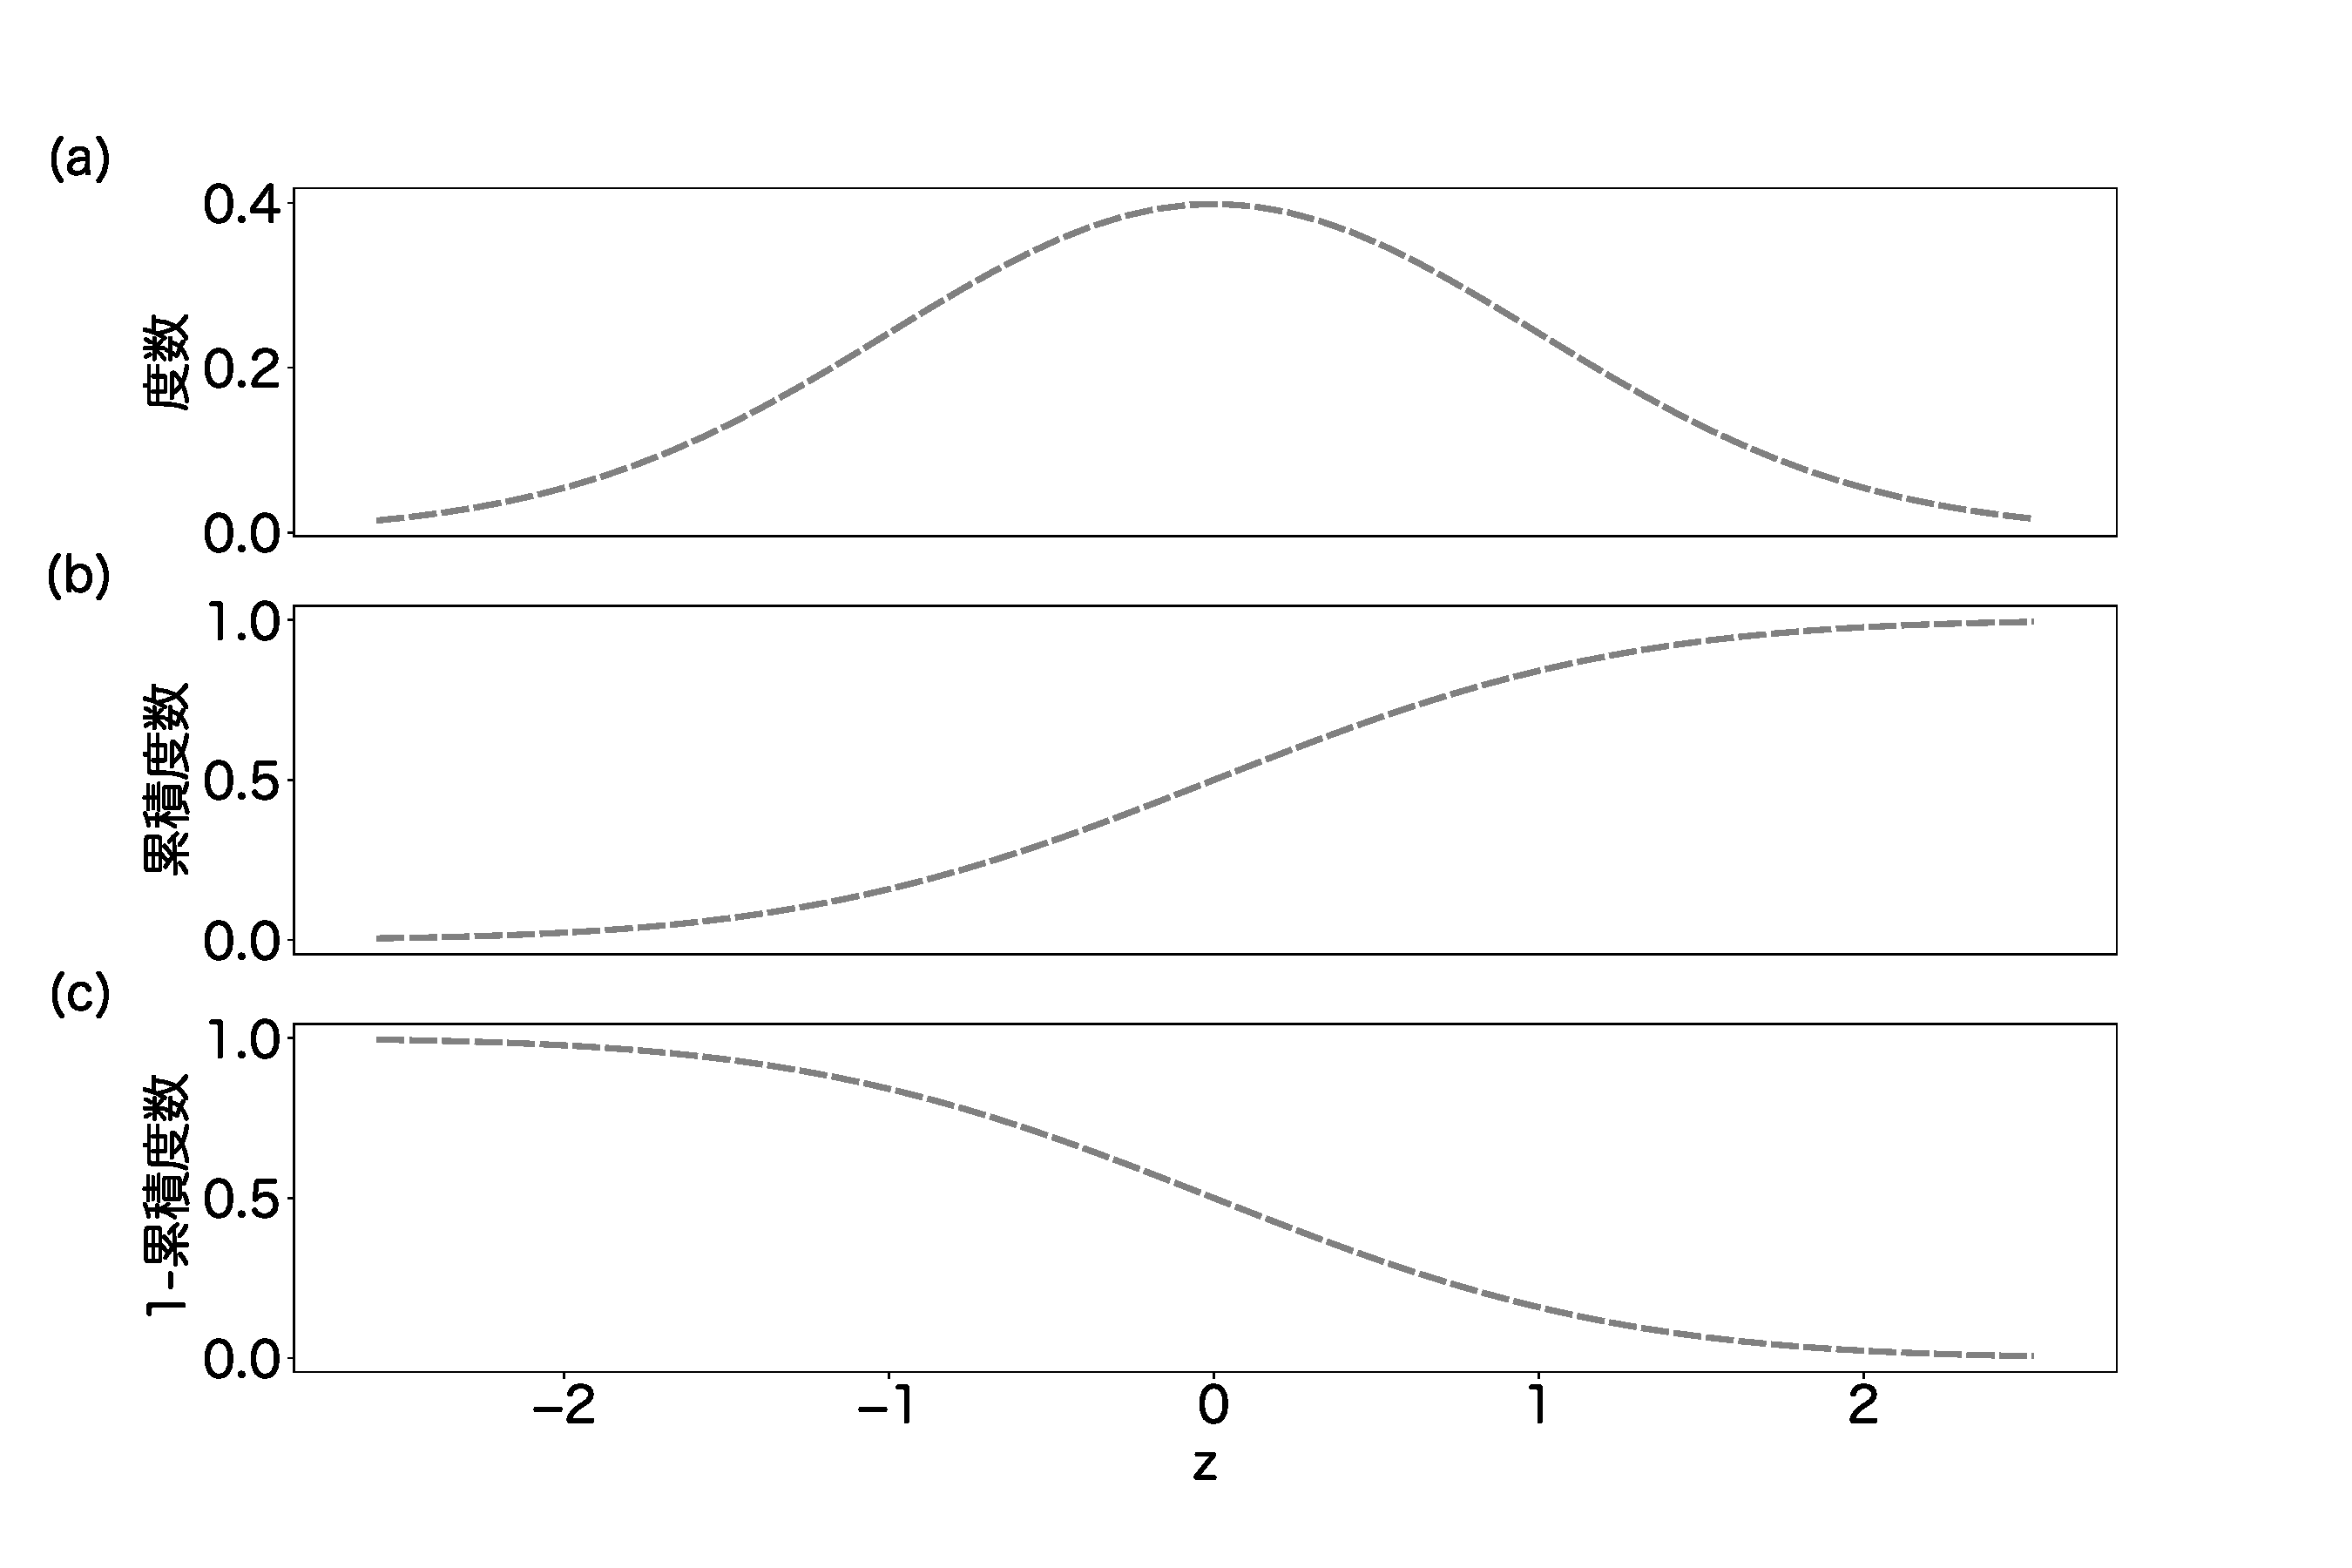
\includegraphics[width=15cm]{../markdown/section1/standard_normal.pdf}
        \caption{標準正規分布(a)確率密度関数(b)累積度数分布(c)1-累積度数分布}
        \label{fig:standard_normal_distribution}

    \end{center}
\end{figure}
    

\subsubsection{正規分布に従う確率変数の出現しやすさ1}
標準正規関数に従う確率変数が$95\%$の確率で見つかる範囲を求めてみます。
標準正規関数は、0を中心にして、対称な関数なので、正負の値が同じ程度の確率で見つかります。言い換えれば、$0\sim a$までの積分値と、$-a\sim 0$までの積分値が同じになります。そこで、次の積分を考えて、その最小値となる値を見つけてみます。
\begin{equation}
\int_{-a}^{a} \frac{1}{\sqrt{2\pi}}\exp(-\frac{z^2}{2}) dz = 0.95
\end{equation}

\begin{lstlisting}
b,a = norm.interval(0.95,0,1) # 積分値が0.95になる範囲を計算
print(norm.cdf(b, loc=0, scale=1)-norm.cdf(a, loc=0, scale=1)) # 0.95になるかを確認
print(b,a) # その範囲を表示
\end{lstlisting}


$0<\alpha<1$に対して、$\Phi(z_\alpha) = 1-\alpha$となる$z_\alpha$を上側$100\%$点という。
$z_{0.05}=1.64,z_{0.025}=1.96$の値は後でよく使う。

より、一般的には、$\alpha(0\leq \alpha \leq 0)$を指定すると、その半分$\alpha/2$となる積分範囲の末端を$a_1$とします。数式で書くと、
\begin{equation}
    \int_{-\infty}^{a_1} \frac{1}{\sqrt{2\pi}}\exp(-\frac{x^2}{2})dx = \frac{\alpha}{2}.
\end{equation}
同様に、右側の範囲の末端を$a_2$とします。数式で書くと、
\begin{equation*}
    \int_{a_2}^{\infty} \frac{1}{\sqrt{2\pi}}\exp(-\frac{x^2}{2})dx = \frac{\alpha}{2}.
\end{equation*}
これを書き換えると、次と同値です。
\begin{equation*}
    \int_{-\infty}^{a_2} \frac{1}{\sqrt{2\pi}}\exp(-\frac{x^2}{2})dx = 1-\frac{\alpha}{2}.
\end{equation*}

\begin{figure}
\begin{center}
    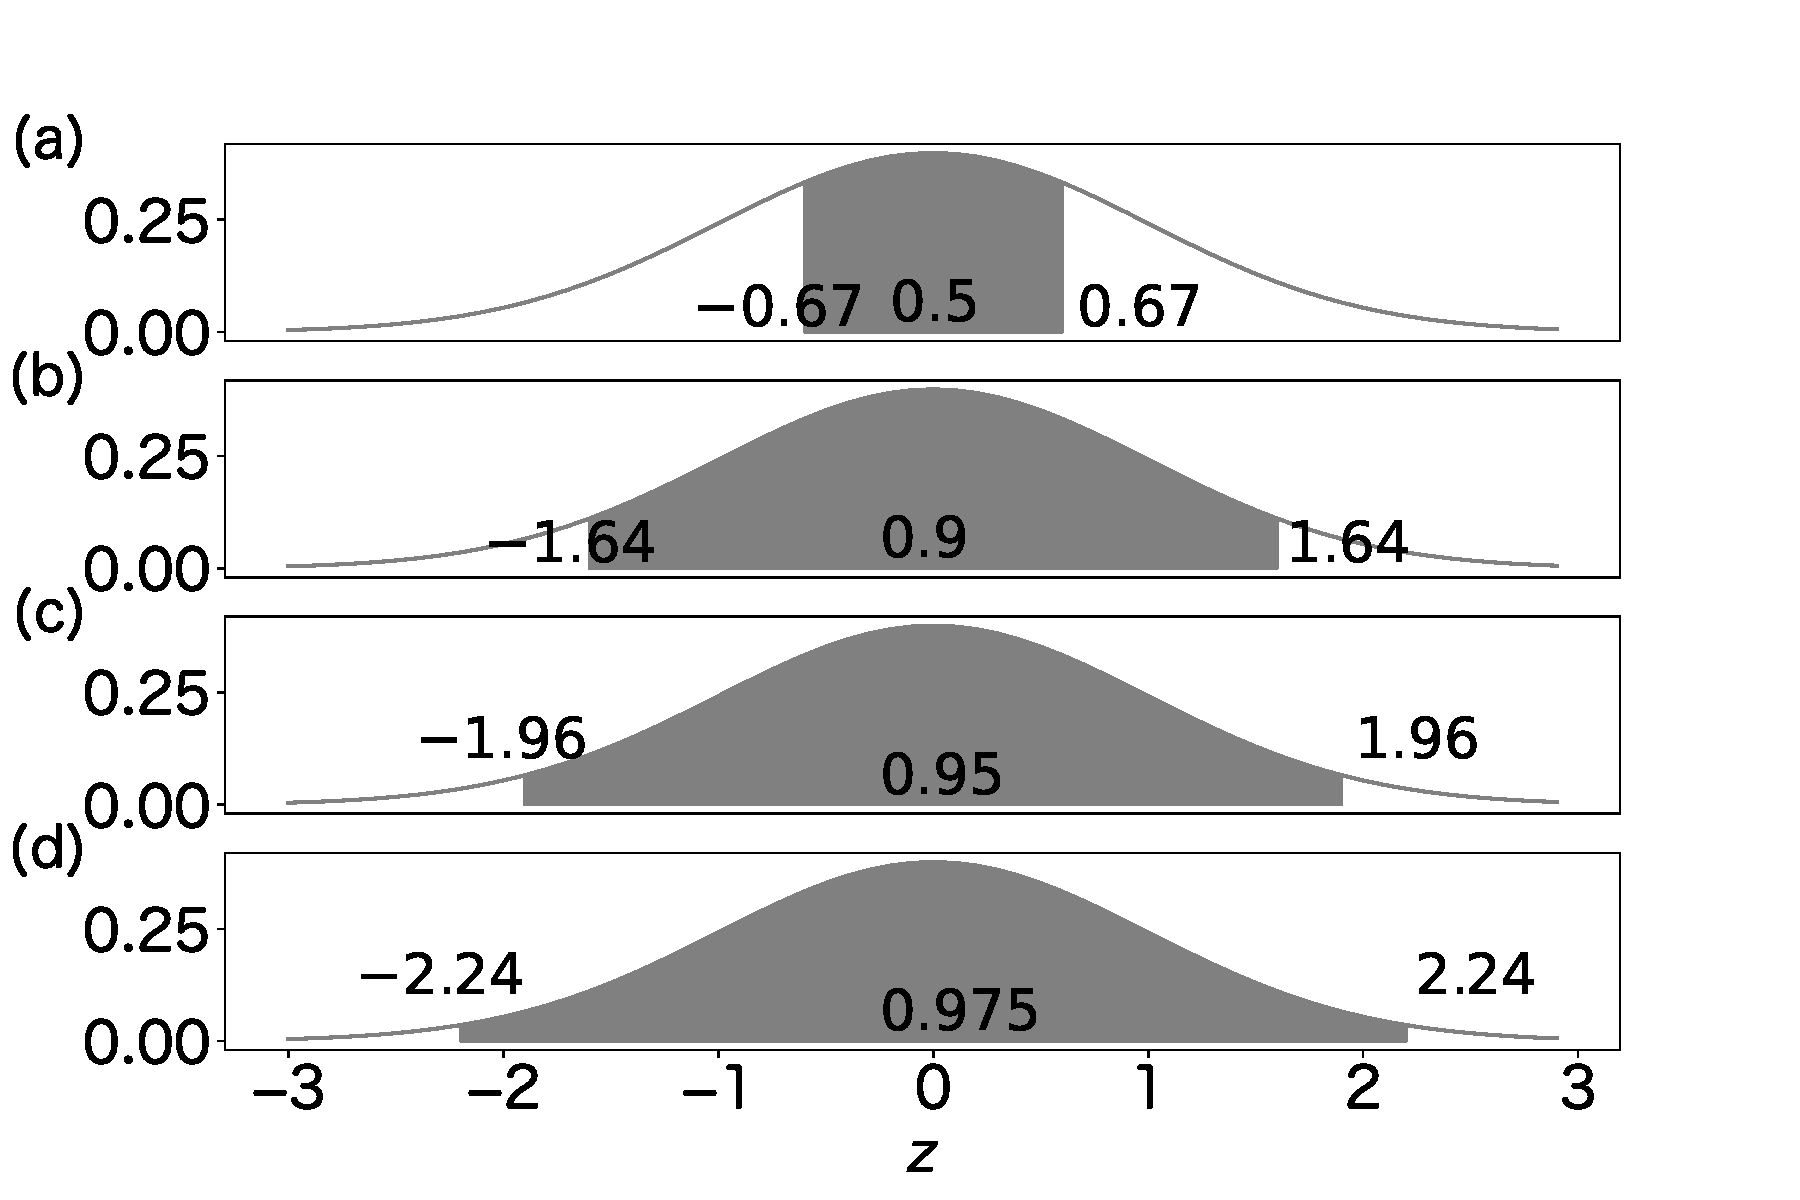
\includegraphics[width=15cm]{../markdown/section1/z_value.pdf}
    %\caption{図1.p値cm}
  \end{center}
\end{figure}

標準正規分布$z\sim N(0,1)$において$95\%$の確率で確率変数が見つかる範囲を調べることはできましたが、正規分布$x\sim N(\mu,\sigma^2)$においてでは、どの範囲になるのでしょう。次の定理を使えば簡単に計算ができます。
\begin{theo}
    確率変数$x$が、$x\sim N(\mu,\sigma^2)$であるならば、$\frac{x-\mu}{\sigma}\sim N(0,1)$である。    
\end{theo}
\begin{theo}
$\alpha(0\leq \alpha\leq 1)$に対して、$\int_{-\infty}^{z}\frac{1}{\sqrt{2\pi}}\exp(-x^2/2)=\alpha$を満たすとき、$\int_{-\infty}^{\mu+\sigma z} \frac{1}{\sqrt{2\sigma^2}}\exp(-\frac{(x-\mu)^2}{2\sigma})=\alpha$である。同様に、$\int_{z}^{-\infty}\frac{1}{\sqrt{2\pi}}\exp(-x^2/2)=1-\alpha$を満たす$z$について、$\int_{\mu+\sigma z}^{\infty} \frac{1}{\sqrt{2\sigma^2}}\exp(-\frac{(x-\mu)^2}{2\sigma})=1-\alpha$である。
\end{theo}
言い換えれば、標準正規分布の軸上の点$z$を、$[-\infty,z]$の範囲での積分値を保ったまま、正規分布$N(\mu,\sigma^2)$上の点に変換するには、$\frac{x-\mu}{\sigma}=z$を$x$について解けば良いことになります。

この定理により、以下をとけば、値が$95\%$の確率で得られる範囲がわかります。
\begin{eqnarray*}
    \frac{x-\mu}{\sigma}=z_{0.025}\\
    \rightarrow x = \mu+\sigma z_{0.025}
\end{eqnarray*}
また、
\begin{eqnarray*}
    \frac{x-\mu}{\sigma}=-z_{0.025}\\
    \rightarrow x = \mu-\sigma z_{0.025}
\end{eqnarray*}
以上により、$x \sim N(\mu,\sigma^2)$が$95\%$の確率で見つかる範囲は、$[\mu-\sigma z_{0.025},\mu+\sigma z_{0.025}]$であることがわかります。
同様に$90\%$の確率で見つかる範囲は、$[\mu-\sigma z_{0.05},\mu+\sigma z_{0.05}]$です。

\subsubsection{より大きな値をとる確率}
$x$を標準正規分布の確率変数とし、($x\sim N(0,1)$)また、$x\leq 0$であるとします。。$x$以上の大きな値を取る確率は、$P(X>x)=1-\varPhi(x)$で計算できます。
同様に、$x < 0$であるときは、より小さな値を取る値が、$P(x<X)=\varPhi(x)$で同様に計算できます。
図\ref{fig:z_value_larger}には、$x$に対して、より異なった値を取る確率を書いています。

$x$の大きさ$|x|$よりも大きな値を取る確率は、以上の二つの和で次のようにかけます。
\begin{equation}
    P(|x|>z) = 1-\varPhi(|x|)+\varPhi(-|x|)
\end{equation}
式を見ると正の数で$x$より大きな値を取る確率と、負の数で$x$より小さな値を取る確率の和になっていることが確認できます。
$P(|x|>z)$はより極端な値を取る確率などと言う方もされます。

計算してみます。$x=1.64$であれば、$\varPhi(1.64)=0.95$より、それ以上に大きな値を得る確率は、$P(X>1.64)=0.05$です。また、$x=-1.64$であれば、$\varPhi(-1.64)=0.05$です。よって、$|x|=|1.64|$よりも大きな値を得る確率は$P(|1.64|>X)=0.1$です。


\begin{figure}
    \begin{center}
        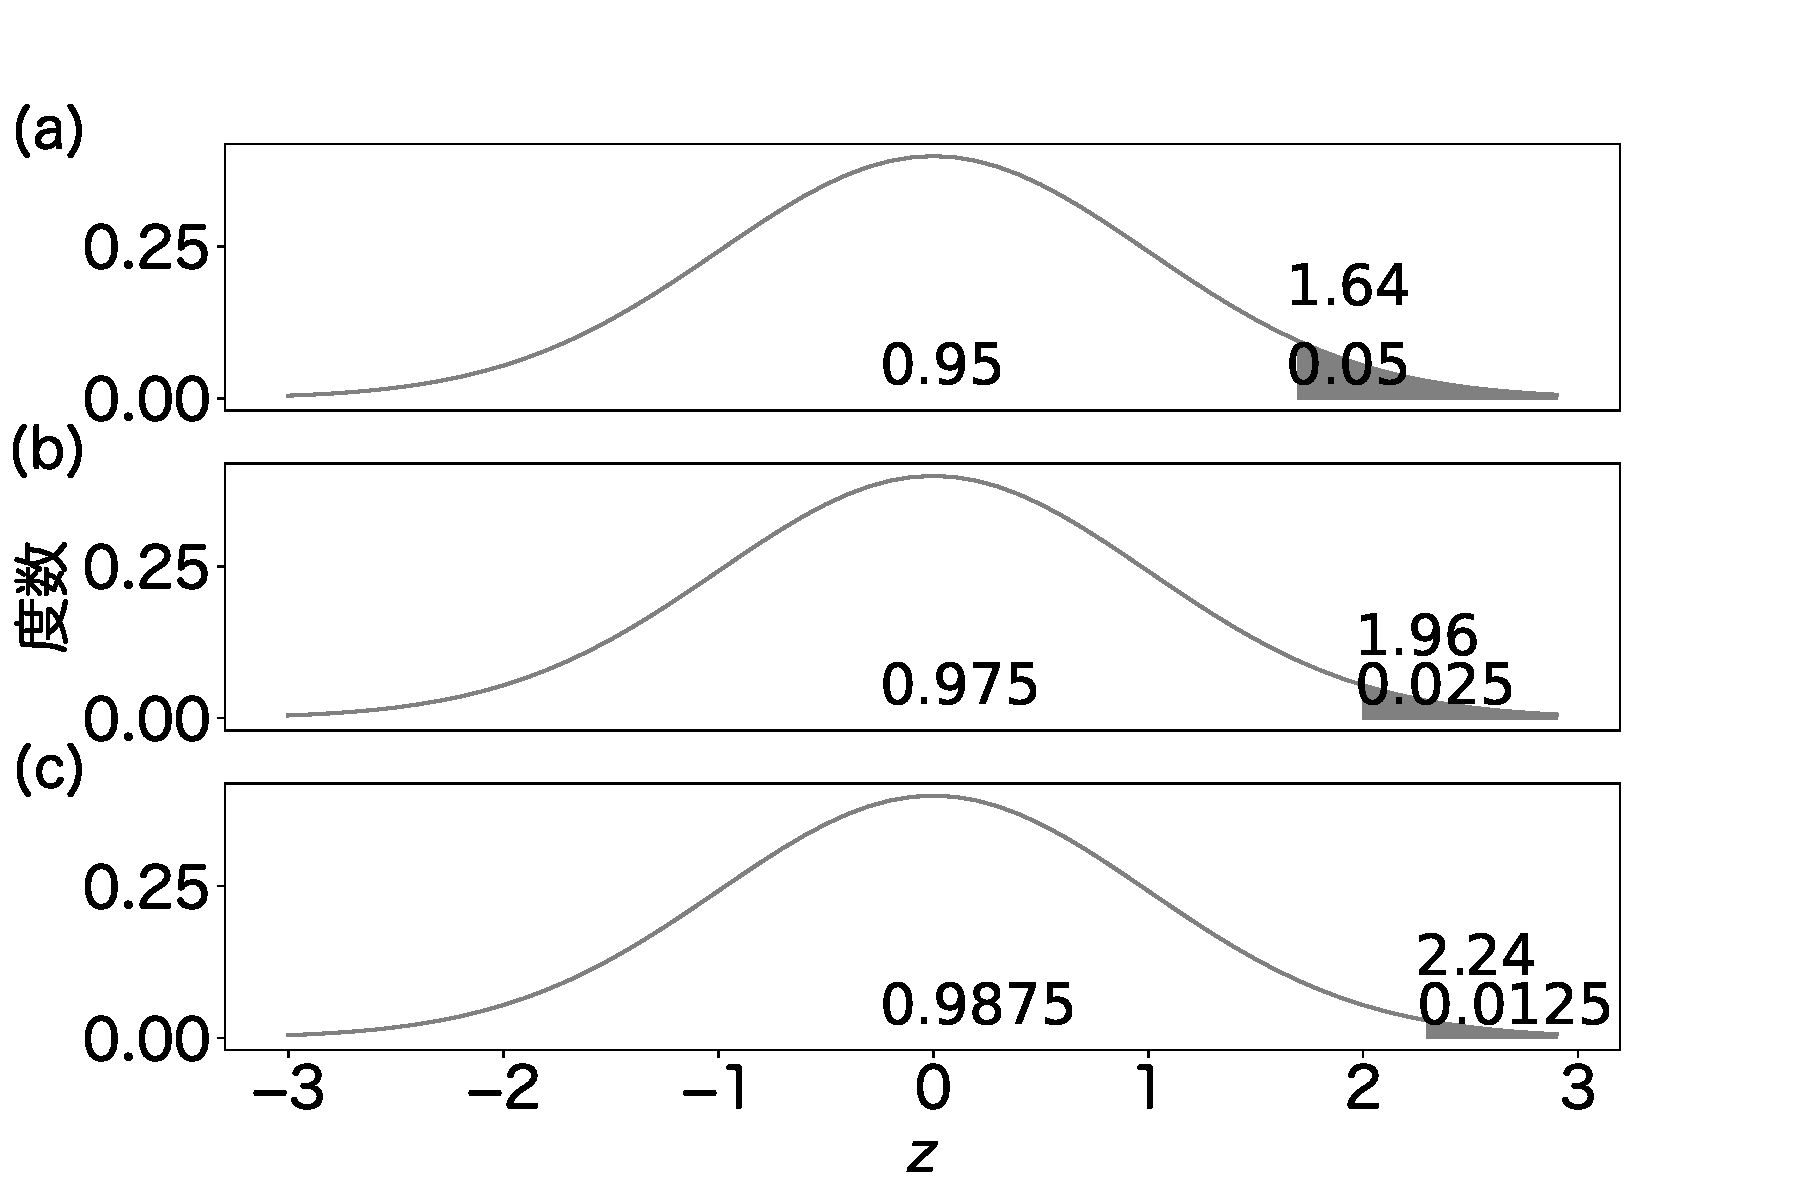
\includegraphics[width=15cm]{../markdown/section1/z_value_larger.pdf}
        \caption{標準正規分布におけるより大きな値(より偏った値)を取る確率。(a)$z=1.64$より大きな値を取る確率は0.05。(b)$z=1.96$より大きな値を取る確率は$0.025$。(c)$z=2.24$よりも大きな値を取る確率は$0.0125$}
        \label{fig:z_value_larger}
      \end{center}
    \end{figure}

\subsubsection{$N(0,1)$での珍しい値は、$N(0,2)$では珍しくない?}
以上の議論により、$N(0,1)$において、$z=1.64$以上の値が出る確率はおよそ$5\%$である。
では、$N(0,2)$において$z=1.64$が出る確率はいくつだろうか。
$N(0,2)$において、$z=1.64\times2$以上に大きな値が出る確率は、およそ$5\%$である。
このことから、$N(0,2)$において$z=1.64$以上の値が出る確率は、$5\%$より大きいことがわかる。
具体的に、計算をしてみると、その確率は$0.206$程度であることがわかる。
\begin{lstlisting}
1-norm.cdf(1.64,0,2)
\end{lstlisting}

\subsubsection{$N(1.96,1)$で出てくる値は、$N(0,1)$において珍しい?}
$N(1.96,1)$において、$1.96$以上の値が出る確率は、$50\%$です。明らかに、よく出る値であることがわかります。
一方で、$N(0,1)$においては、$1.96$以上の値が出る確率は、$2.5\%$くらいなので、珍しい値になります。
このように、確率分布の母数が変化すると、珍しい値も変化します。




\subsubsection{正規分布に従う確率変数の出現しやすさ2}
確率変数のしやすさを表す基準として、$\sigma$を基準にして、定数$a$倍の範囲$[\mu-a\sigma,\mu+a\sigma]$を使う方法もあります。
標準正規分布では、分散が$1$なので、その$0.5$倍、$1$倍、$2$倍、$3$倍の範囲はそれぞれ$[-0.5,0.5]$,$[-1,1]$,$[-2,2]$,$[-3,3]$になります。この範囲に入る確率は、それぞれ$0.38$,$0.683$,$0.954$,$0.997$です。それぞれの範囲と確率は、図\ref{fig:sigma_interval_probability}に図示しました。

$\sigma$の定数倍の範囲に値が見つかる確率は、$\sigma$の大きさに依存しないことが証明できます。言い換えれば、$[-0.5\sigma,0.5\sigma],[-\sigma,\sigma],[-2\sigma,2\sigma],[-3\sigma,3\sigma]$の範囲に値がある確率は、上記と同じで、それぞれおよそ$0.38$,$0.683$,$0.954$,$0.997$になります。


\begin{figure}
    \begin{center}
        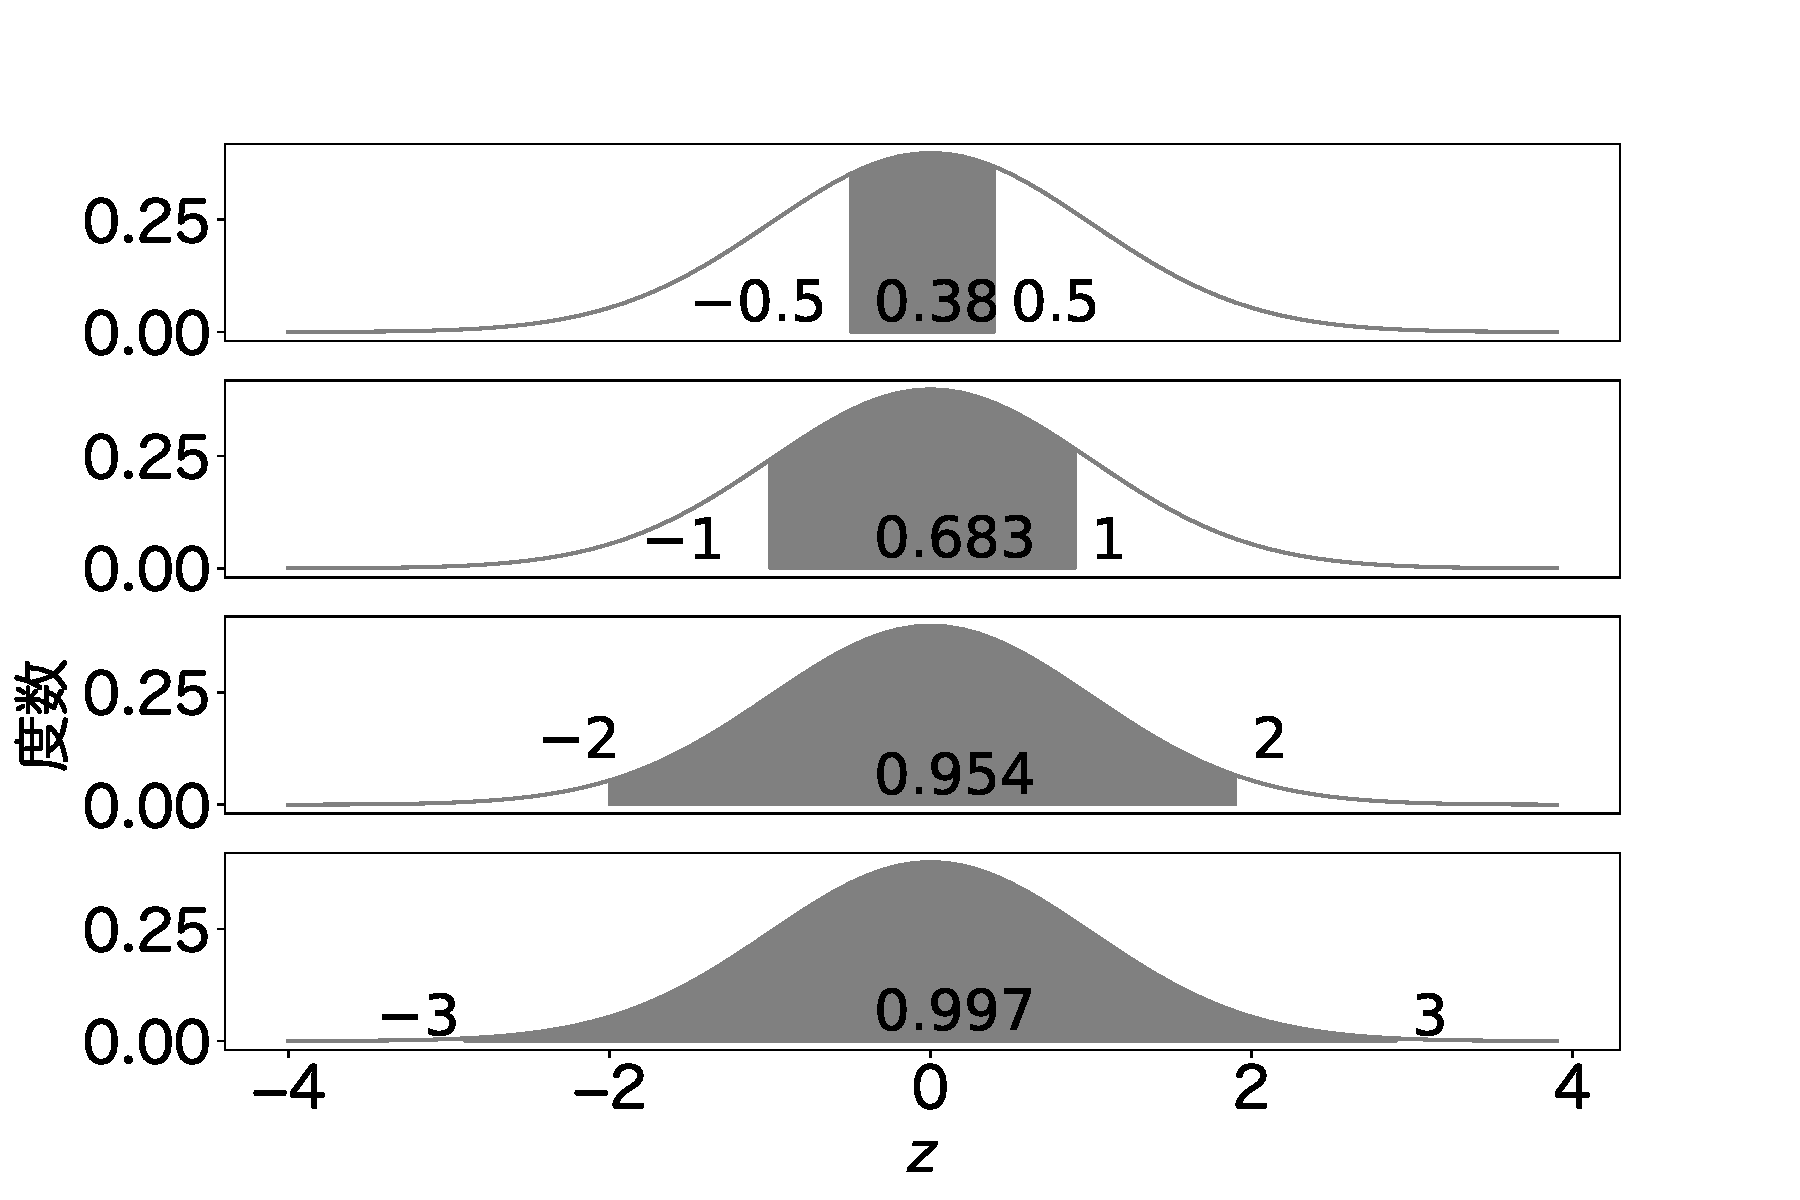
\includegraphics[width=15cm]{../markdown/section1/sigma_value.pdf}
        %\caption{図1.p値cm}
        \label{fig:sigma_interval_probability}
      \end{center}
\end{figure}

\begin{table}[hbtp]
    \caption{$\sigma$を基準にした値の出やすさ}
    %\label{table:data_type}
    \centering
    \begin{tabular}{lcr}
        \hline
        出現確率  & $N(0,1)$  &  $N(\mu,\sigma^2)$ \\
        \hline \hline
        0.38 & [-0.5,0.5]  & $[\mu-0.5\sigma,\mu+0.5\sigma]$ \\
        0.683 & [-1,1] & $[\mu-\sigma,\mu+\sigma]$\\
        0.954 & [-2,2] & $[\mu-2\sigma,\mu+2\sigma]$\\
        0.996 & [-3,3] & $[\mu-3\sigma,\mu+3\sigma]$\\
    \end{tabular}
\end{table}




\subsection{指数分布}
確率変数$X$が指数分布に従うことを$X \sim Exp(\lambda)$と書く。
指数分布の確率密度関数は、
\begin{equation*}
    f(x)=\lambda \exp(-\lambda x).
\end{equation*}
ここで、$\lambda$は、$\lambda>0$であり、指数分布の母数である。
期待値は$E[X]=\frac{1}{\lambda}$で、分散は、$V[X]=\frac{1}{\lambda^2}$である。
累積分布関数は、
\begin{equation*}
    F(x)=1-\exp(-\lambda x).
\end{equation*}
正規分布は、母数平均を中心として、左右対称に分布していた。言い換えれば、$\phi(\mu+x)=\phi(\mu-x)$である。一方で、指数分布は、左右非対称に分布が広がり、小さな値は大きな値よりも出現確率が高いので、$f(E[X]+a)\neq f(E[X]-a)$である。
また、正規分布では、母数平均と母数分散がそれぞれ独立なので、それぞれの特徴を独立に動かすことで、期待値や分散が独立に変化する。
指数分布では、母数が一つであり、母数を変化させると、期待値と分散は同時に変化する。



\begin{figure}
    \begin{center}
        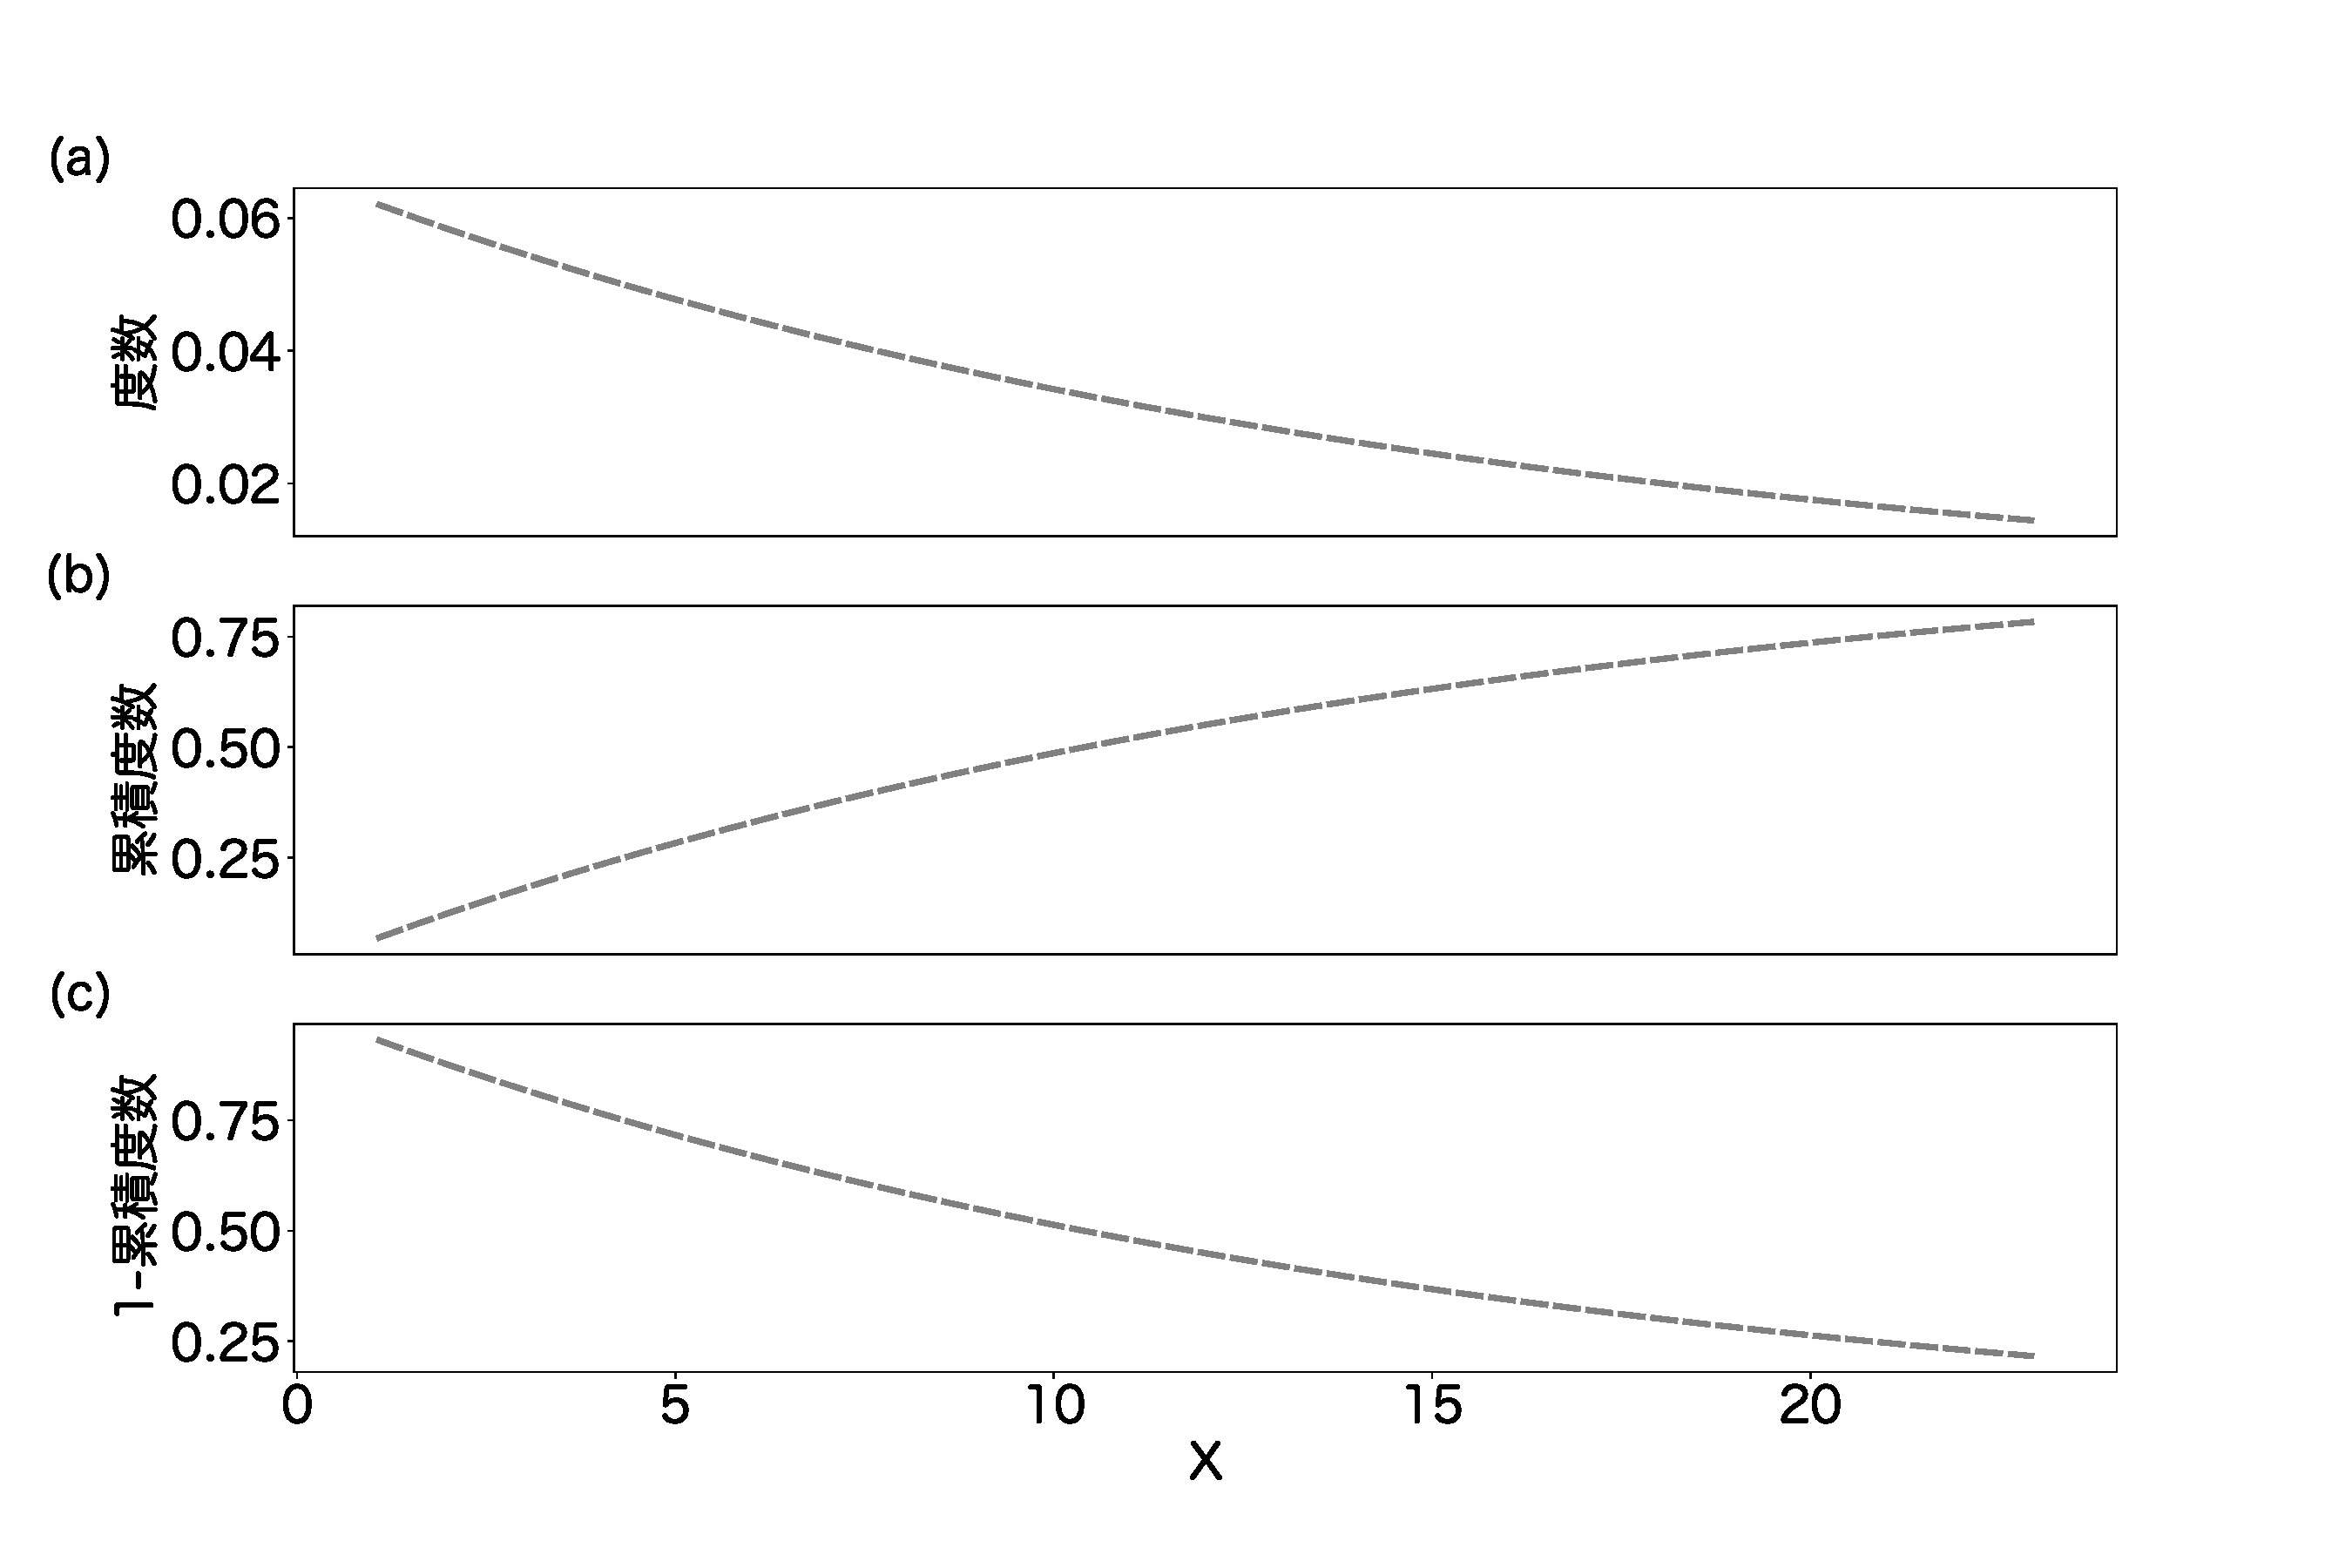
\includegraphics[width=15cm]{../markdown/section1/expon_frequency.pdf}
        \caption{指数分布$\lambda=1/15$(a)確率密度関数(b)累積度数分布(c)相補累積度数分布}
        \label{expon_frequency}
    \end{center}
\end{figure}


\subsubsection{指数分布に従う確率変数の出現しやすさ}
指数分布の確率密度関数を区間$[a,b]$で積分したときに、$\alpha(0\leq \alpha \leq 1)$になる$[a,b]$を求めます。条件として、
\begin{eqnarray*}
    \int_0^{a}  \lambda\exp(-\lambda x )dx &=& \alpha/2\\
    \int_0^{b} \lambda\exp(-\lambda x )dx &=& 1-\alpha/2
\end{eqnarray*}
を満たすとする。
$a$について、とくと、
\begin{eqnarray*}
    \int_0^{a}  \lambda\exp(-\lambda x )dx &=& \alpha/2\\
     1-\exp(-\lambda a) &=& \frac{\alpha}{2}\\
     \rightarrow a&=& \frac{1}{\lambda} \log\frac{1}{1-\alpha/2}
\end{eqnarray*}
$b$については、同様に、
\begin{equation*}
    b = \frac{1}{\lambda}\log\frac{\alpha}{2}
\end{equation*}
以上より、この積分の条件で、$100(1-\alpha)\%$の確率で値を得る範囲は、$[\frac{1}{\lambda} \log\frac{1}{1-\alpha/2} ,\frac{1}{\lambda}\log\frac{\alpha}{2}]$である。
図\ref{fig:expon_simulation_sample}は、指数分布により、サンプルサイズ$1000$の標本を$100$回作って、各標本においてデータが区間$[\frac{1}{\lambda} \log\frac{1}{1-\alpha/2} ,\frac{1}{\lambda}\log\frac{\alpha}{2}]$に入った割合をシミュレーションし、そのヒストグラムを表示している。確かに、$95\%$くらいの割合でその区間にデータが入っている。


\begin{figure}
    \begin{center}
        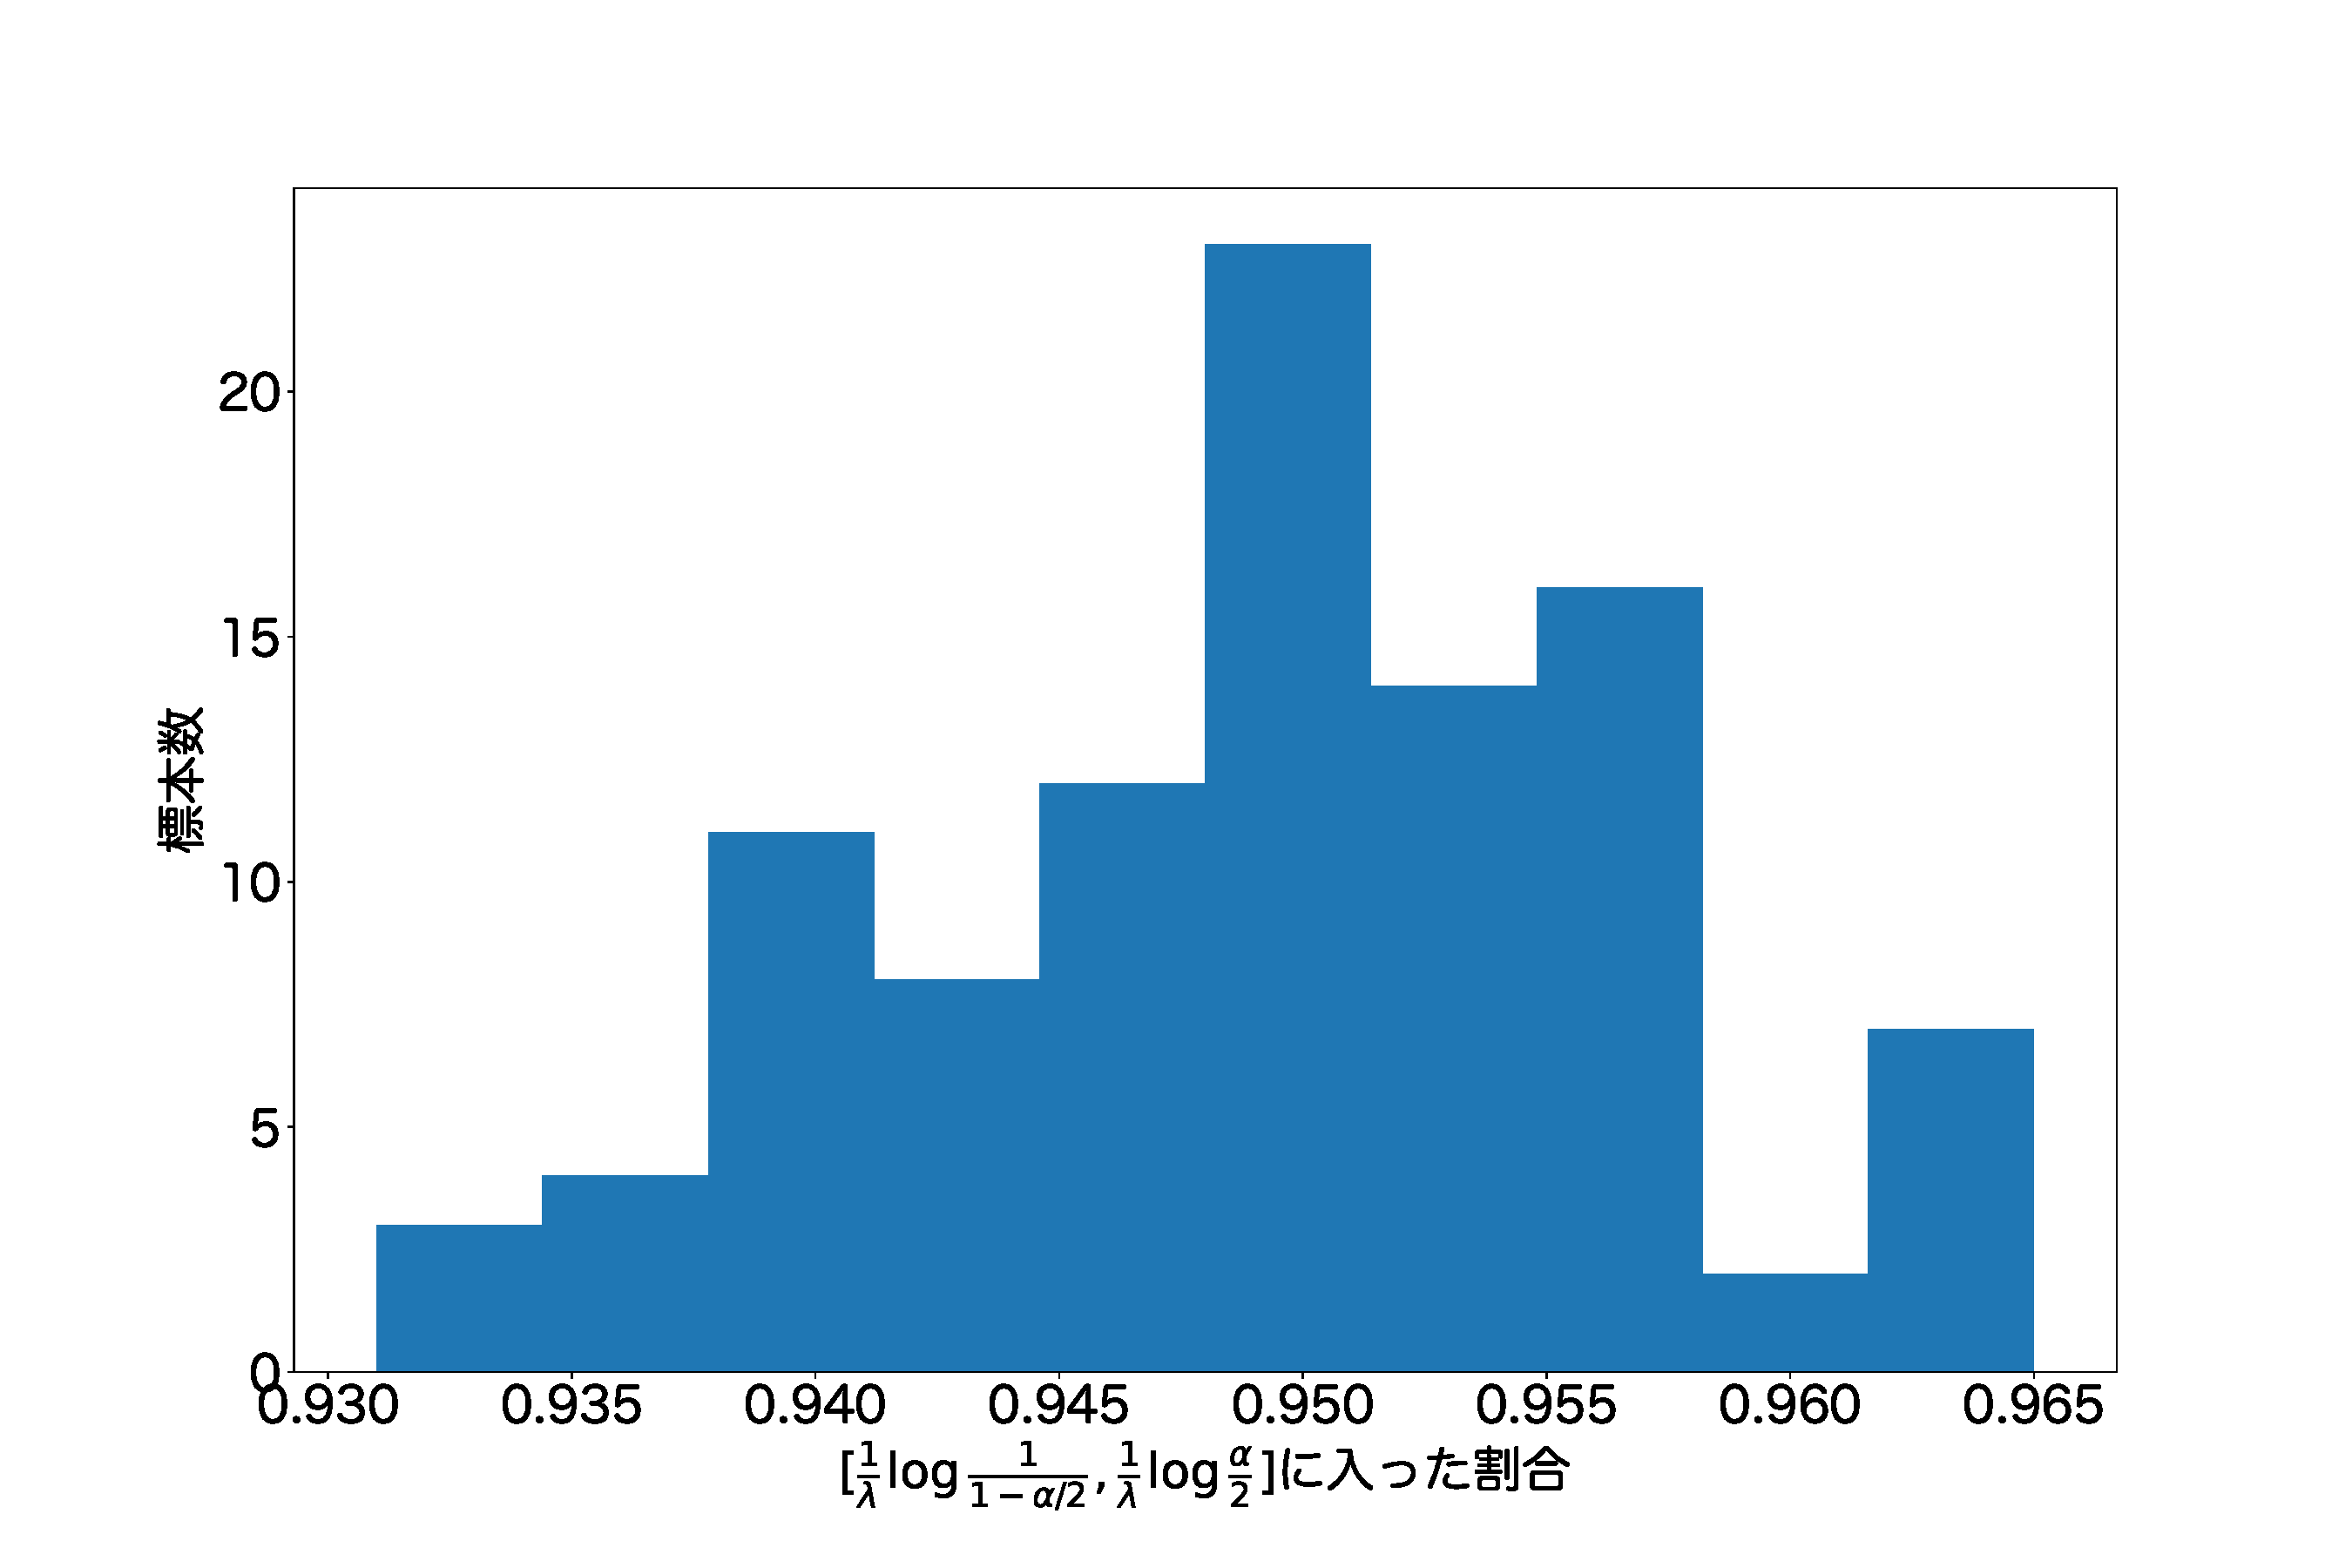
\includegraphics[width=15cm]{../markdown/section1/expon_simulation_sample.pdf}
        \caption{指数分布$\lambda=1/10$からサンプルサイズ1000の標本を100回シミュレーションし、各標本においてデータが区間$[\frac{1}{\lambda} \log\frac{1}{1-\alpha/2} ,\frac{1}{\lambda}\log\frac{\alpha}{2}]$に入った割合を計算した。そのヒストグラム。}
        \label{fig:expon_simulation_sample}

    \end{center}
\end{figure}


\subsection{カイ二乗分布}
確率変数$X$がカイ二乗分布に従うことを$X \sim \chi^2_k$と書く。ここで、$k$はカイ二乗分布の母数で、自由度を示し、自然数を取る。
確率密度関数は、
\begin{equation*}
    f(x;k) = \frac{1}{2^{k/2}\Gamma(k/2)}x^{k/2-1}\exp\left(-\frac{x}{2}\right).
\end{equation*}
ここで、$\Gamma(k/2)$はガンマ関数を表す\footnote{$ \Gamma(z)=\int_0^{\infty }t^{z-1}\exp(-t)dt$である。 }。
累積分布間数は、
\begin{equation*}
    F(x) = \frac{\gamma(k/2,x/2)}{\Gamma(k/2)}.
\end{equation*}
ここで、$\gamma(k/2,x/2)$は、不完全ガンマ関数である\footnote{$\gamma(a,x)=\int_0^x t^{a-1}\exp^{-t}dt$である。ガンマ関数も、不完全ガンマ関数も計算できなくても問題はない。コンピュータを使えばすぐに計算してくれる。}。
この関数も左右非対称である。


\begin{figure}
    \begin{center}
        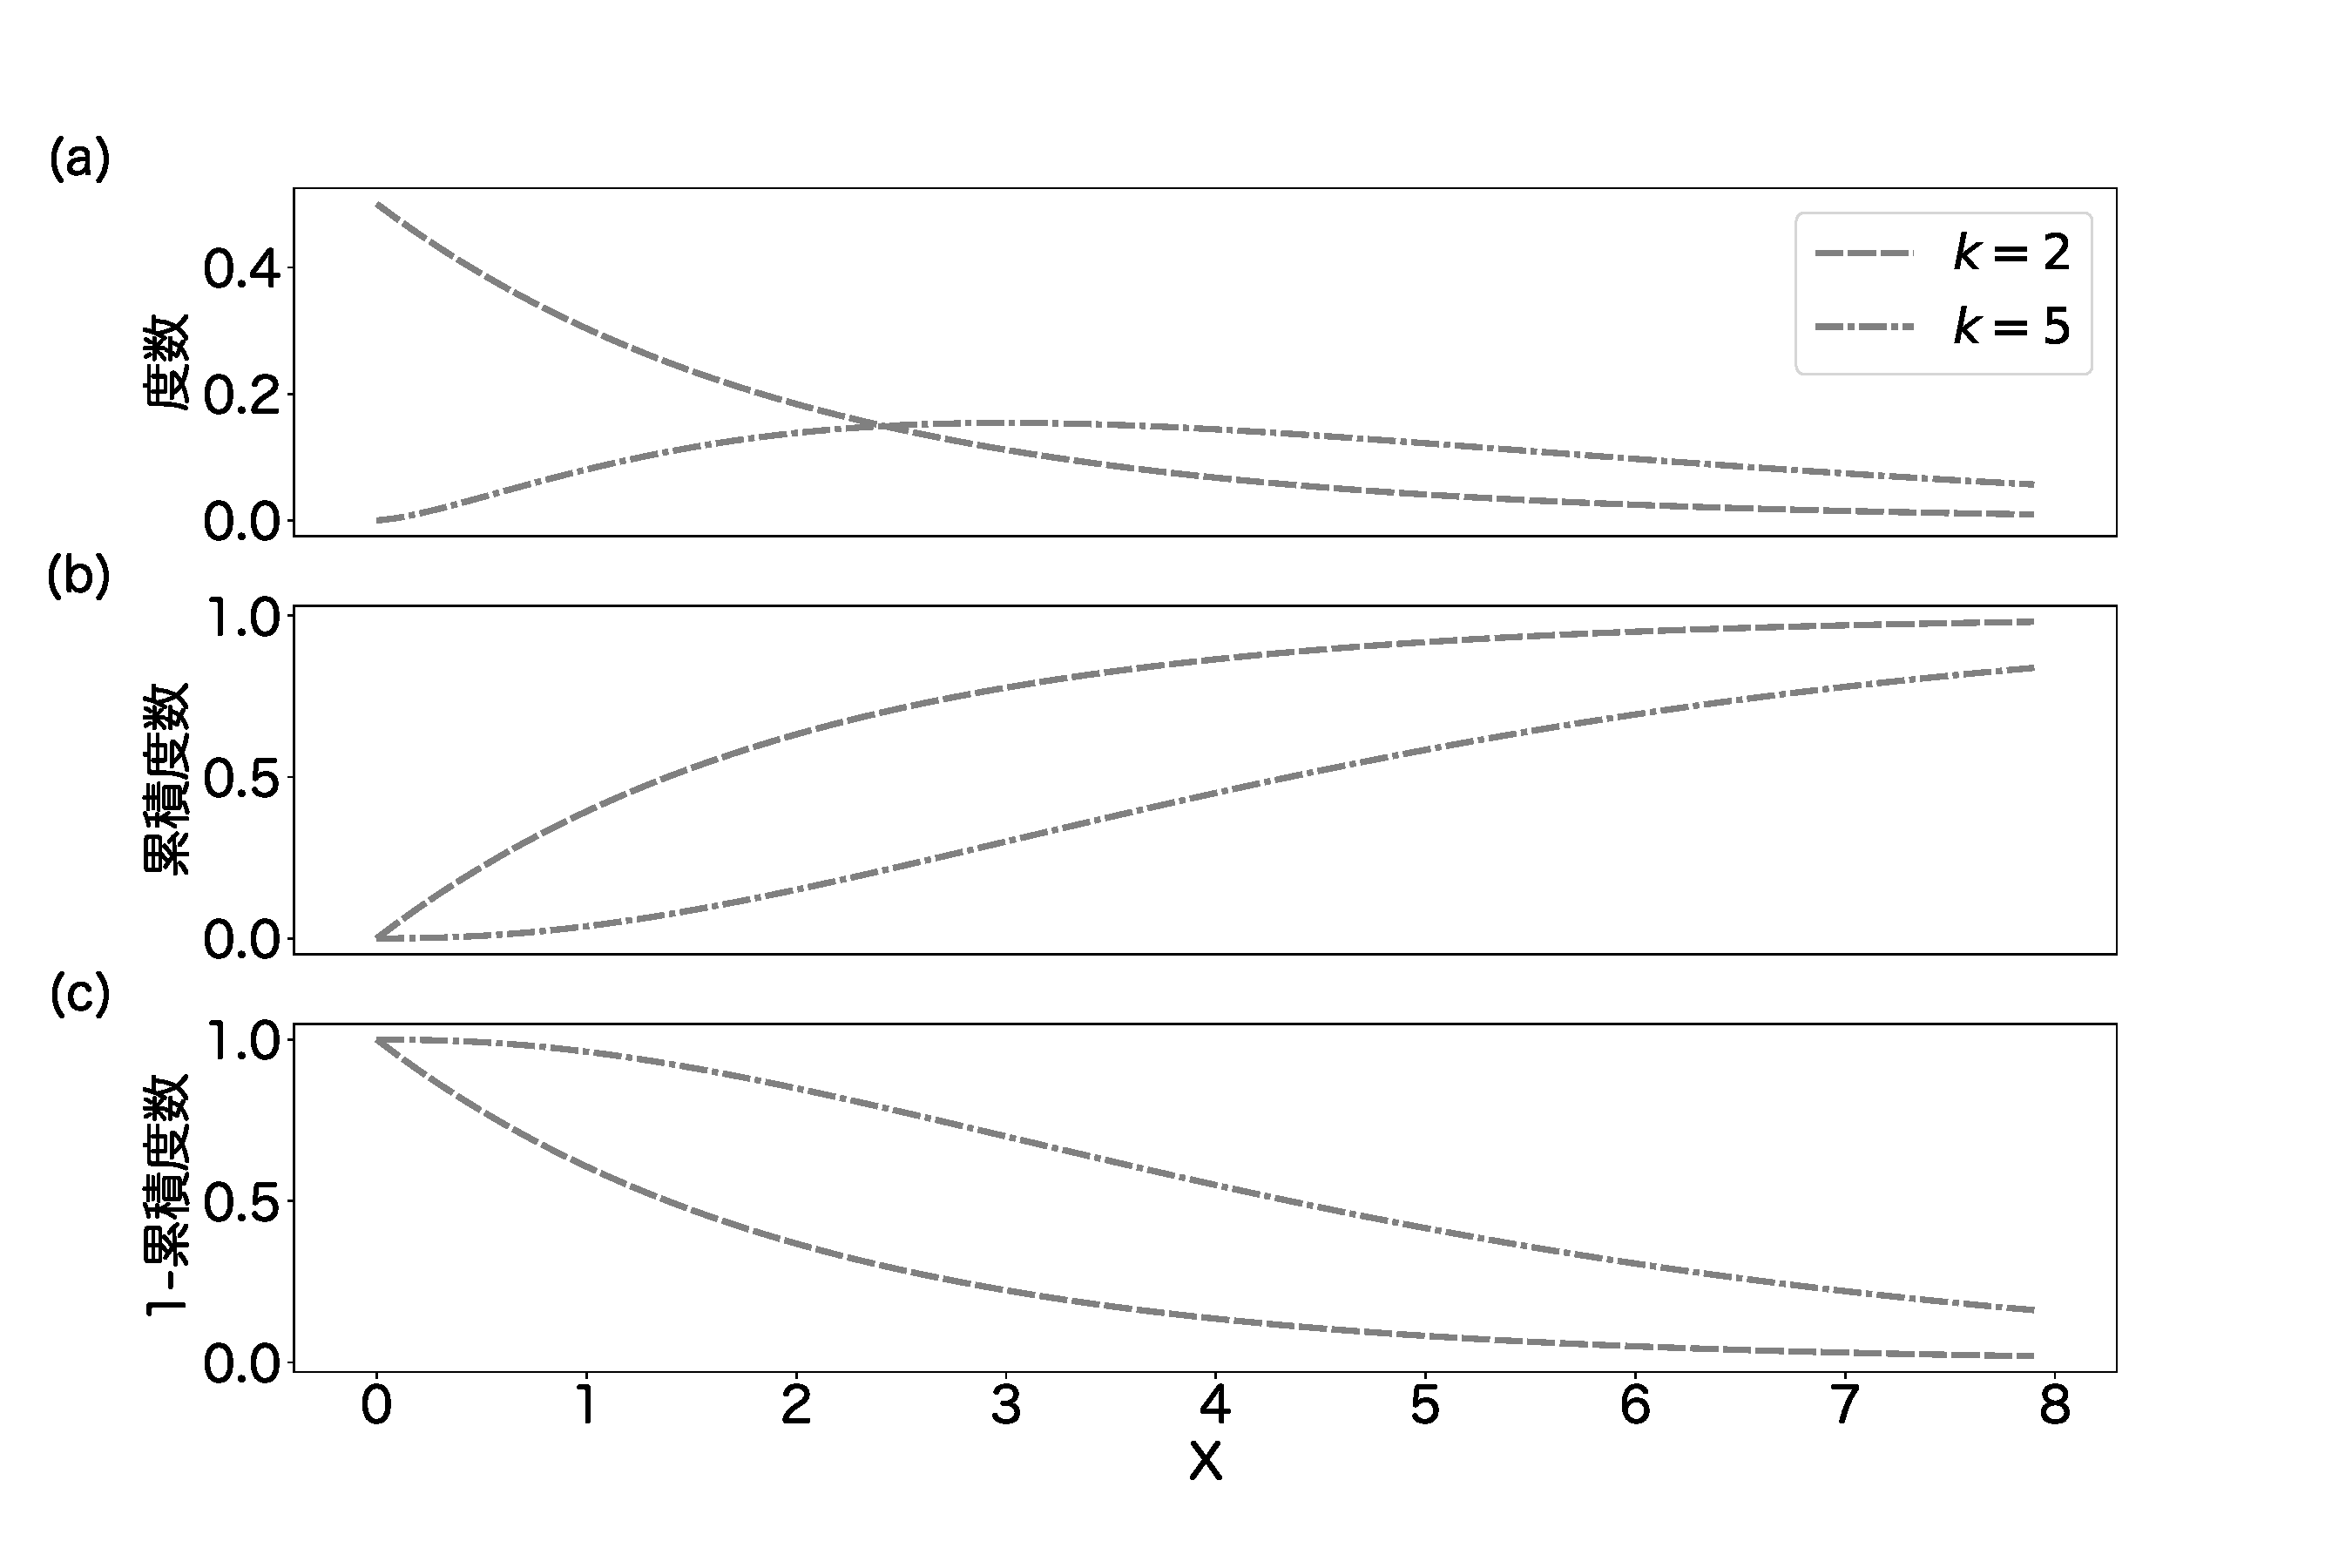
\includegraphics[width=15cm]{../markdown/section1/chi2_frequency.pdf}
        \caption{カイ二乗分布}
        \label{chi2_}
    \end{center}
\end{figure}

\subsubsection{カイ二乗分布に従う確率変数の出現しやすさ}
カイ二乗分布の確率密度関数を区間$[a,b]$で積分したときに、$\alpha(0\leq \alpha \leq 1)$になる$[a,b]$を求めます。条件として、
\begin{eqnarray*}
    \int_0^{a}  \frac{1}{2^{k/2}\Gamma(k/2)}x^{k/2-1}\exp\left(-\frac{x}{2}\right)dx &=& F(a)-F(0) = \alpha/2\\
    \int_0^{b} \frac{1}{2^{k/2}\Gamma(k/2)}x^{k/2-1}\exp\left(-\frac{x}{2}\right)dx &=& F(b)-F(0)= 1-\alpha/2
\end{eqnarray*}
を満たすとする。
代数的に$a,b$について解くことが難しいので、数値的に計算してみた結果を載せておく(表\ref{table:chi2_confidence})。この$a,b$をそれぞれ$\chi^2_k(\alpha),\chi^2_{k}(1-\alpha)$と書くことがある。


\begin{table}[hbtp]
    \caption{$\alpha=0.05$}
    \label{table:chi2_confidence}
    \centering
    \begin{tabular}{lcc}
    %\hline
    k  & $a$   & $b$   \\
    \hline \hline
    1 &  0.0009 &  5.02\\
    3 & 0.215 & 9.3484  \\
    5 &  0.831 & 12.832 \\
      \hline
    \end{tabular}
  \end{table}

\subsection{$t$分布}
確率変数$T$が$t$分布に従うとき、$T \sim t(\nu)$と表記する。
確率密度関数は、
\begin{equation*}
    f(t) = \frac{\Gamma((\nu+1)/2)}{\sqrt{\nu \pi}\Gamma(\nu/2) }(1+t^2/\nu)^{-(\nu+1)/2}.
\end{equation*}
ここで、$\nu$は、$0$より大きな実数である。
この関数を見ただけでは、すぐには判別するのは難しいかもしれないが、$f(t)$には$t$が関係する部分は$(1+t^2/\nu)$だけである。二乗の項があるので、偶数関数であることがわかり、$0$を中心にした対称な関数$f(t)=f(-t)$であることがわかる。
累積分布関数は著者には難しすぎるので、記述しない。wikipediaなどで調べれば正しそうな数式が書かれている。



\begin{figure}
    \begin{center}
        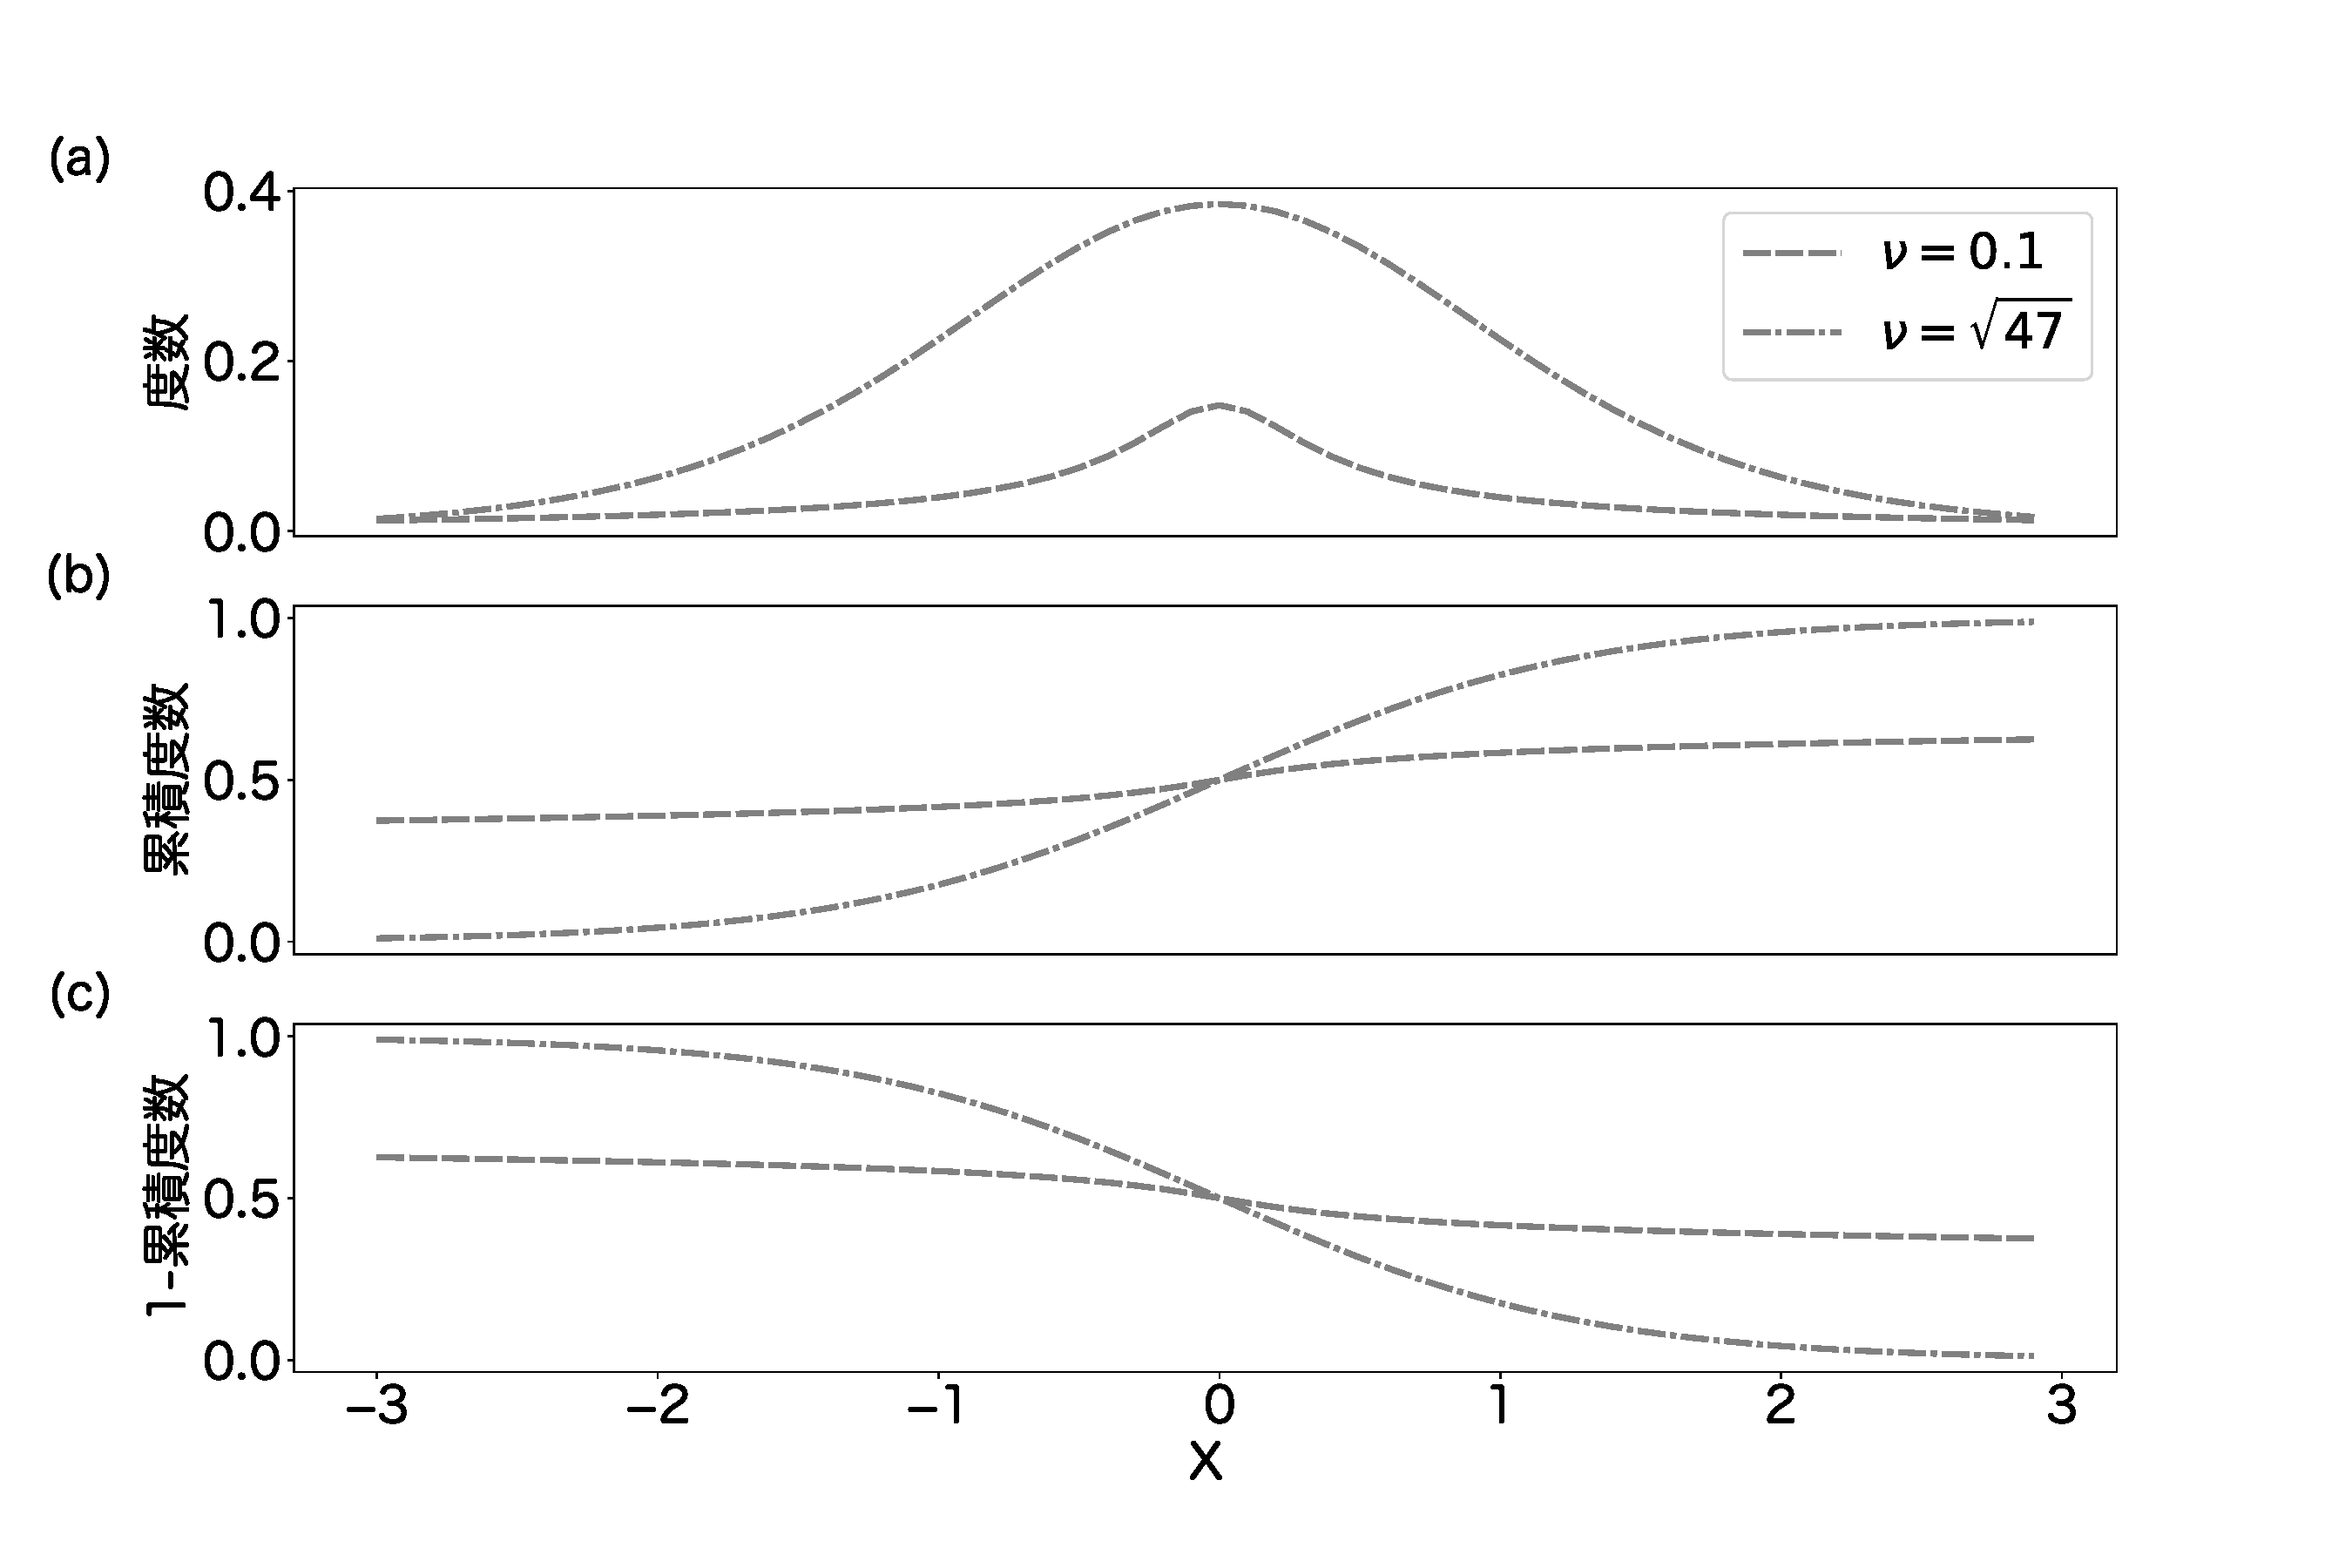
\includegraphics[width=15cm]{../markdown/section1/student_t_frequency.pdf}
        \caption{t分布}
        \label{student_t}
    \end{center}
\end{figure}

\subsubsection{$t$分布における珍しい値}
$t$分布における$|T|$以上の値が得られる確率が$\alpha$程度になる$|T|$のリスト。
例えば、$n=10$の$t$分布において$|T|=1.81$以上の値が得られる確率は、$0.1$程度である。


\begin{table}[hbtp]
    \caption{$t$分布における$|T|$以上の値が得られる確率が$\alpha$程度になる$|T|$のリスト}
    \label{table:student_t_confidence}
    \centering
    \begin{tabular}{cccc}
    %\hline
    n & p=0.1 & $p=0.05$ & $p=0.025$   \\
    \hline \hline
    1 & 6.31 & 12.70 & 25.45 \\
    5 & 2.01 &2.57  & 3.16\\
    10 & 1.81 &  2.22& 2.63 \\
      \hline
    \end{tabular}
  \end{table}
% https://bellcurve.jp/statistics/course/8968.html


\subsection{統計分布の関係}
同一の確率分布からサンプリングされた複数の確率変数$X_1,X_2,\cdots,X_n$を得たとき、それを要約した要約統計量がどのような分布関数に従うのかを考察する。
% $(\star)$のついた項目は、科学的(恣意的)な判断を含んでいる。

\subsubsection{正規分布の再生性}
$X \sim N(\mu_1,\sigma^2_1),Y\sim(\mu_2,\sigma^2_1)$とするとき、$aX+bY \sim N(a\mu_1+b\mu_2,a^2\sigma^2_1+b^2\sigma^2_2)$より、$a=\frac{1}{2},b=\frac{1}{2}$。すると、$\frac{X}{2}+\frac{Y}{2}\sim N(\frac{\mu_1+\mu_2}{2},\frac{\sigma^2_1}{2^2}+\frac{\sigma^2_2}{2^2})$である。$\mu_1=\mu_2,\sigma_1=\sigma_2$とすると、$\frac{X+Y}{2}\sim N(\mu_1,\frac{\sigma^2_1}{2})$が成り立つ。
このことを利用すると、$X_1,X_2,\cdots,X_n\sim N(\mu,\sigma^2)$とすると、$\bar{X}=\frac{X_1+X_2+\cdots+X_n}{n}\sim N(\mu,\frac{\sigma^2}{n})$である。よって$\frac{\bar{X}-\mu}{\sqrt{\frac{\sigma^2}{n}}}\sim N(0,1) $。また、$\bar{x}$の出現しやすい区間は、
\begin{equation*}
    -z_{0.025}<\frac{\bar{X}-\mu}{\sqrt{\frac{\sigma^2}{n}}} < z_{0.025}
\end{equation*}
である。式を変形すると、
\begin{equation*}
    \mu-z_{0.025}\frac{\sigma^2}{n}<\bar{x}<\mu+z_{0.025}\frac{\sigma^2}{n}
\end{equation*}
がわかる。
以上をまとめておく。

\begin{theo}
    $X_1,X_2,\cdots,X_n \sim N(\mu,\sigma^2)$とすると、$\frac{\bar{X}-\mu}{\sqrt{\frac{\sigma^2}{n}}}\sim N(0,1)$ ただし、$\bar{X}=\frac{X_1+X_2+\cdots+X_n}{n}$。また、$\bar{X}$の出現しやすい区間は、$\mu-z_{0.025}\frac{\sigma^2}{n}<\bar{x}<\mu+z_{0.025}\frac{\sigma^2}{n}$である。
\end{theo}



\begin{theo}
    $X_1,X_2,\cdots,X_{n_1} \sim N(\mu_1,\sigma_1^2),Y_1,Y_2,\cdots,Y_{n_2}\sim N(\mu_2,\sigma_2^2)$ただし、$\mu_1\neq \mu_2,\sigma_1\neq \sigma_2$とする。正規分布の再生性により、$\bar{X}\sim N(\mu_1,\frac{\sigma^2_1}{n_1}),\bar{Y}\sim N(\mu_2,\frac{\sigma^2_2}{n_2})$である。次が成り立つ。
    $\bar{X}-\bar{Y} \sim N(\mu_1-\mu_2,\frac{\sigma^2_1}{n_1}+\frac{\sigma^2_2}{n_2})$であり、
    \begin{equation*}
        \frac{(\bar{X}-\bar{Y})-(\mu_1-\mu_2)}{\sqrt{\frac{\sigma_1^2}{n_1}+ \frac{\sigma_2^2}{n_2}}}\sim N(0,1).
    \end{equation*}
\end{theo}



\subsubsection{指数分布の再生性}
指数分布$Exp(\lambda)$と、ガンマ分布$Ga(1,\frac{1}{\lambda})$は、同一の密度分布関数であり、それは$f(x) = \frac{1}{\lambda} \exp(-\frac{x}{\lambda})$である。ガンマ分布には、分布の再生性があり、$X\sim Ga(a_1,b),Y\sim Ga(a_2,b)$であるなら、$X+Y \sim Ga(a_1+a_2,b)$である。このことを、$n$個の確率変数$X_1,X_2,\cdots X_n \sim Exp(\lambda)(=Ga(1,\frac{1}{\lambda}) )$に適用すると、$X_1+X_2+\cdots+X_n \sim Ga(n,\frac{1}{\lambda})$である。以上によって、$n\bar{X}\sim Ga(n,\frac{1}{\lambda})$ただし、$\bar{X}=X_1+X_2+\cdots+X_n$である。
再生性については、確率母関数を利用することで証明できる。

\begin{theo}
    $X_1,X_2,\cdots,X_n \sim Ga(1,\frac{1}{\lambda})$ならば、
    $n\bar{X}\sim Ga(n,\frac{1}{\lambda})$
\end{theo}

\begin{proof}
    $Ga(1,\frac{1}{\lambda})$の確率母関数は、$M_X(t)=(1-\frac{1}{\lambda}t)^{-1}$である。確率変数$X_1+X_2+\cdots+X_n$の確率母関数は
    \begin{eqnarray}
        M_{n\bar{X}} = M_{X_1+X_2+\cdots+X_n} &=& M_{X_1}M_{X_2}\cdots M_{X_n} \\
        &=& (1-\frac{1}{\lambda}t)^{-1}(1-\frac{1}{\lambda}t)^{-1}\cdots(1-\frac{1}{\lambda}t)^{-1}\\
        &=& (1-\frac{1}{\lambda}t)^{-n}
    \end{eqnarray}
    以上より、$n\bar{x}\sim Ga(n,\frac{1}{\lambda})$である。
\end{proof}

\if 0
\subsubsection{対数正規分布の再生性}
$X\sim \Lambda(\mu_1,\sigma_1^2), Y\sim \Lambda(\mu_2,\sigma^2_2)$とするとき、$XY\sim\Lambda(\mu_1+\mu_2,\sigma_1^2+\sigma_2^2)$である。
これを使えば、$X_1,X_2,\cdots,X_n \sim \Lambda(\mu,\sigma^2)$について、その積$X_1,X_2\cdots X_n \sim \Lambda(n\mu,n\sigma^2)$である。

ここで、$X_1X_2\cdots X_n$は十分統計量にならないので、検定が作れないのか?
一方で、$\log X_1+\log X_2 \cdots \log X_n $は十分統計量$N(\mu,\sigma^2)$に従う。
$\log X_1^2+\log X_2^2 \cdots \log X_n $は十分統計量$\chi^2$分布に従う
% https://stats.stackexchange.com/questions/202890/jointly-sufficient-statistic-question
% https://mcm-www.jwu.ac.jp/~konno/pdf/statr28.pdf
% https://www.stats.ox.ac.uk/~reinert/stattheory/solutions109.pdf
% https://pages.stern.nyu.edu/~wgreene/MathStat/old-exam-1.pdf
% https://math.stackexchange.com/questions/3597198/sketching-power-function-for-a-log-normal-density
% https://stats.stackexchange.com/questions/402522/likelihood-ratio-test-of-log-normal-distribution
% https://abicky.net/2014/03/03/202054/
\fi

\subsubsection{正規分布とt分布の関係}
$X_1,X_2,\cdots,X_n \sim N(\mu,\sigma^2)$とする。統計量$T$を、
\begin{equation*}
    T = \frac{\bar{X}-\mu}{\sqrt{\frac{S^2}{\sqrt{n}}}}.
\end{equation*}
ここで、$\bar{X}=\frac{X_1+X_2+\cdots+X_n}{n}$、$S^2=\frac{1}{n-1}\sum_{i=1}^{n}(X_i-\bar{X})^2$である。
この統計量$T$は、$t(n-1)$分布に従うことが知られている。統計量$T$の中に母数$\sigma$が入っていないので、$\sigma$わからないときでも、$T$を計算すれば、それが$t(n-1)$に従うことがわかる。

2つの正規分布$X_1,X_2,\cdots,X_{n_1} \sim N(\mu_1,\sigma_1^2), Y_1,Y_2,\cdots,Y_{n_2}\sim N(\mu_2,\sigma_1^2)$とする。このとき、
\begin{equation*}
    T = \frac{(\bar{X}-\bar{Y})-(\mu_1-\mu_2)}{\sqrt{\frac{U^2}{n_1}+\frac{U^2}{n_2}}}
\end{equation*}
は、$n_1+n_2-2$の$t$分布に従う。ここで、$U$は、
\begin{equation*}
    U^2 = \frac{(n-1)U_1^2+(n_2-1)U_2^2}{n_1-1+n_2-1}
\end{equation*}
であり、$U_1,U_2$は、不偏分散
\begin{eqnarray*}
    U_1^2 = \frac{1}{n_1-1}\sum_{i=1}^{n_1}(X_i-\bar{X})\\
    U_2^2 = \frac{1}{n_2-1}\sum_{i=1}^{n_2}(Y_i-\bar{Y})\\
\end{eqnarray*}
である。

\section{問題意識}
確率変数$x_1$または、$x_1,x_2,\cdots,x_n$を得たとき、それらが独立同分布に従うという前提のもと、ある母数をもつ分布関数に従う、または従わないと推測することは可能であるだろうか。
最尤推定から、確率変数を得たなら、最尤推定を行って、母数を推測可能な場合がある。
具体的には、正規分布から得られた確率変数については、その平均と分散は、$(\mu,\sigma^2)=(\bar{x},\sum_{i=1}^{n} (x_i-\bar{x})^2/n)$である。

この問題に対して、
正規分布から確率変数を得たとき、ある母数平均$\mu$をもつ正規分布からサンプリングされていないということはできるだろうか。これを議論する。

%\subsection{言葉の準備}


\subsection{ひとつの確率変数から推測する}
ひとつの確率変数$x$が$N(\mu,\sigma^2)$に従わないことを推定したい。
$N(\mu,\sigma^2)$から得られる確率変数は、$95\%$の確率で、$\mu-\sigma z_{0.025}\sim \mu-\sigma z_{0.025}$の間で見つかる。
$\sigma^2=1$とすると、$95\%$の確率で、確率変数は、$\mu-1.96\sim\mu+1.96$の間で見つかる。
$\mu=0$なら、$x=0.1$は、この区間の中にあるので、$x$は、$N(0,1)$では良く見つかる値になる。
%この基準では、複数の$\mu$で$x=0.1$はよく見つかる範囲に入る。例えば、$\mu=0.1$でも良く確率変数が見つかる区間は、$-1.85\sim 2.05$なので、確率変数は、$N(0.1,1)$に従うとしても問題ない。
$x=0.1$がその区間に入らない母数は、$\mu=z_{0.025}+0.1$のときで、区間は$0.10003\sim4.01$で、この区間に$x$は入ってません。
これを言い換えれば、母数$x-z_{0.025}\leq\mu\leq x+z_{0.025}$の間でよくある値になり、この間から外れた母数をもつ$N(\mu,1)$に従っていいないと推測できる。

我々の科学では、このようなたったひとつの値から、分布関数の母数を推測することはしません。
例えば、$x=1.97$が得られたとすると、$N(0,1)$のよく出る値の範囲は、$-1.96\sim1.96$であることから、母数$0$ではないと判断できます。
一方で、$N(0,1)$で$x=1.97$は、サンプルサイズが$20$であれば、そのうち$1$回は、$1.97$をとる値です。もしももう一度サンプリングできたとして、その値が$0$になることもあり得ます。
以上のことから、$1$回のサンプリングだけで判断しません。

\subsection{複数の確率変数から推測する}
複数の確率変数$x_1,x_2,\cdots,x_n$が$N(\mu,\sigma^2)$に従わないことを推定したい。

サンプルサイズが大きいときは、最尤推定を行い、$\mu_1=\bar{x},\sigma_1^2=\sum_{i=1}^{n} (x_i-\bar{x})^2/n$を計算し、その値が、$\mu,\sigma^2$と著しく異なっていれば、$N(\mu,\sigma^2)$に従わないと言えそうである。
例えば、図\ref{fig:maximum_likelihood_0}は、正規分布$N(170,6.8^2)$からサンプルサイズ$100$の標本を得たとき、図\ref{fig:maximum_likelihood_1}は、サンプルサイズ$30$、そしてそのデータの分布と、最尤推定量から予測されるも確率密度関数、$N(168,6.8^2),N(171,6.8^2)$を表している。図\ref{fig:maximum_likelihood_0}をみると、最尤推定した確率密度関数がデータの出現頻度をよく表していること、そして、周辺の二つの正規分布$N(168,6.8^2),N(171,6.8^2)$とデータが乖離していることがわかる。
一方、図\ref{fig:maximum_likelihood_1}では、データが$N(171,6.8^2)$に従っているのではないかという疑惑が残る。

\begin{figure}
    \begin{center}
        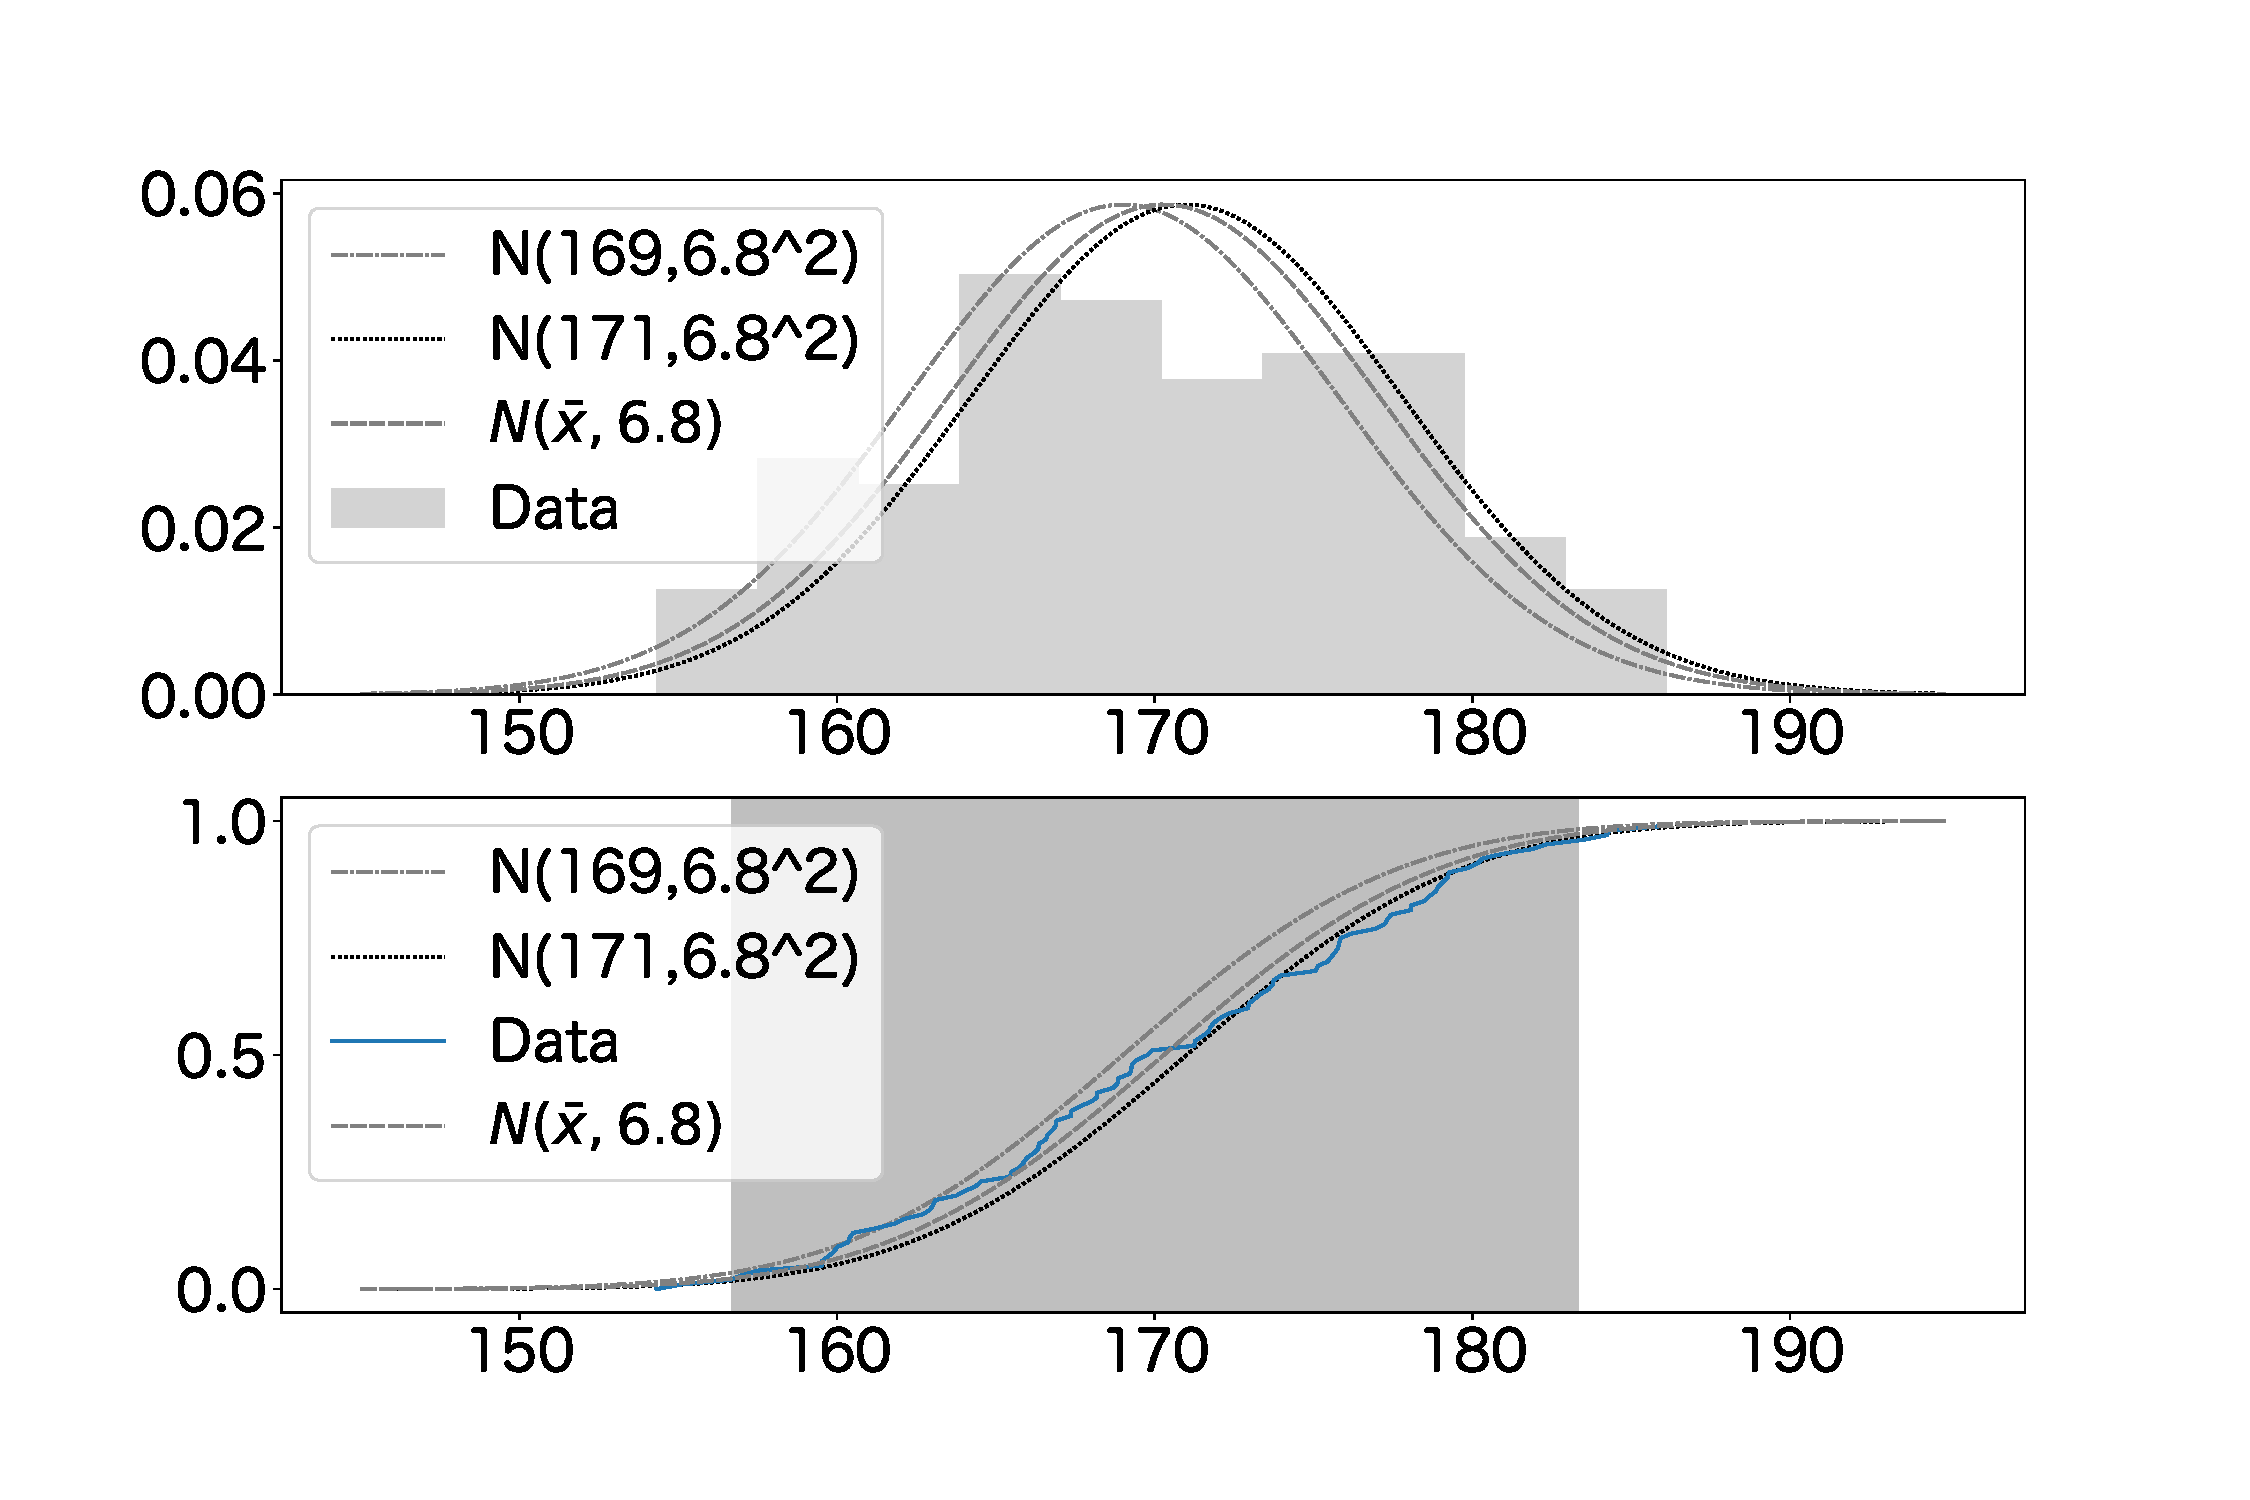
\includegraphics[width=15cm]{../markdown/section1/maximum_likelihood_0.pdf}
        \caption{$N(170,6.8^2)$からサンプルサイズ$100$の標本を得たときの分布。その最尤推定量により求められる分布関数。$N(168,6.8^2),N(171,6.8^2)$の分布関数を示す}
        \label{fig:maximum_likelihood_0}
    \end{center}
\end{figure}
\begin{figure}
    \begin{center}
        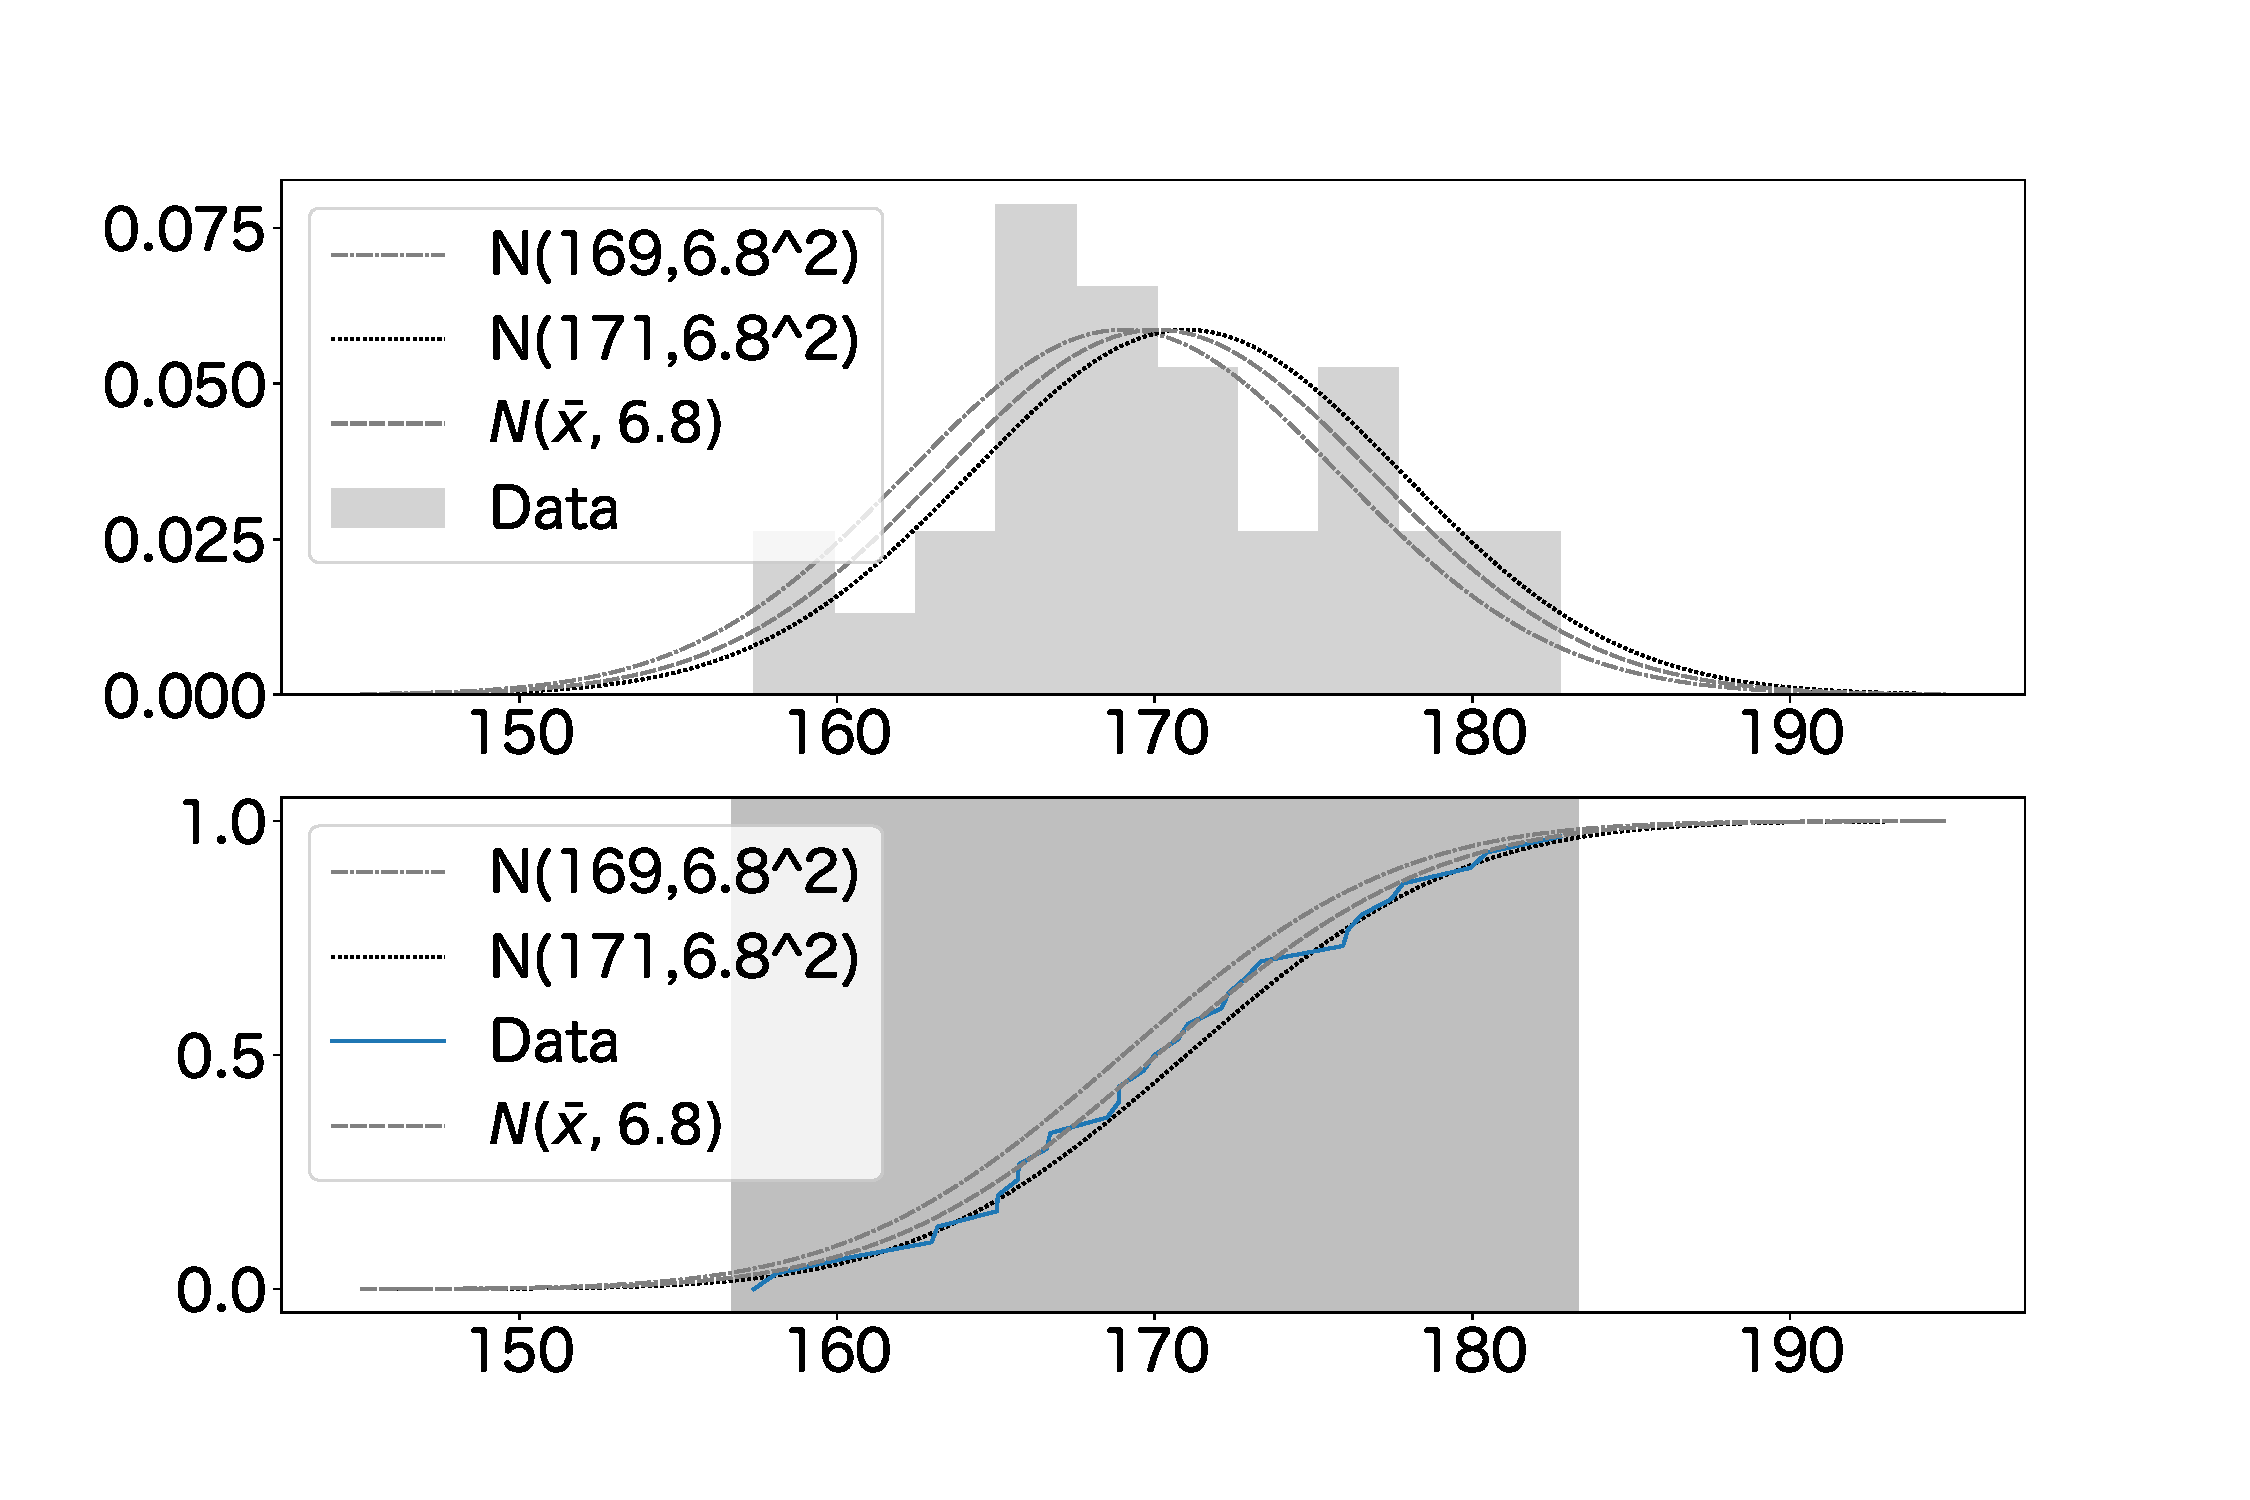
\includegraphics[width=15cm]{../markdown/section1/maximum_likelihood_1.pdf}
        \caption{$N(170,6.8^2)$からサンプルサイズ$30$の標本を得たときの分布。その最尤推定量により求められる分布関数。$N(168,6.8^2),N(171,6.8^2)$の分布関数を示す}
        \label{fig:maximum_likelihood_1}
    \end{center}
\end{figure}

このように、サンプルサイズが大きいと、最尤推定により推測した確率密度関数を見れば、そのほかの母数に従わないことがわかる場合がある。
また、より近くにある母数の確率密度関数と区別することは難しいこともわかる。

\begin{figure}
    \begin{center}
        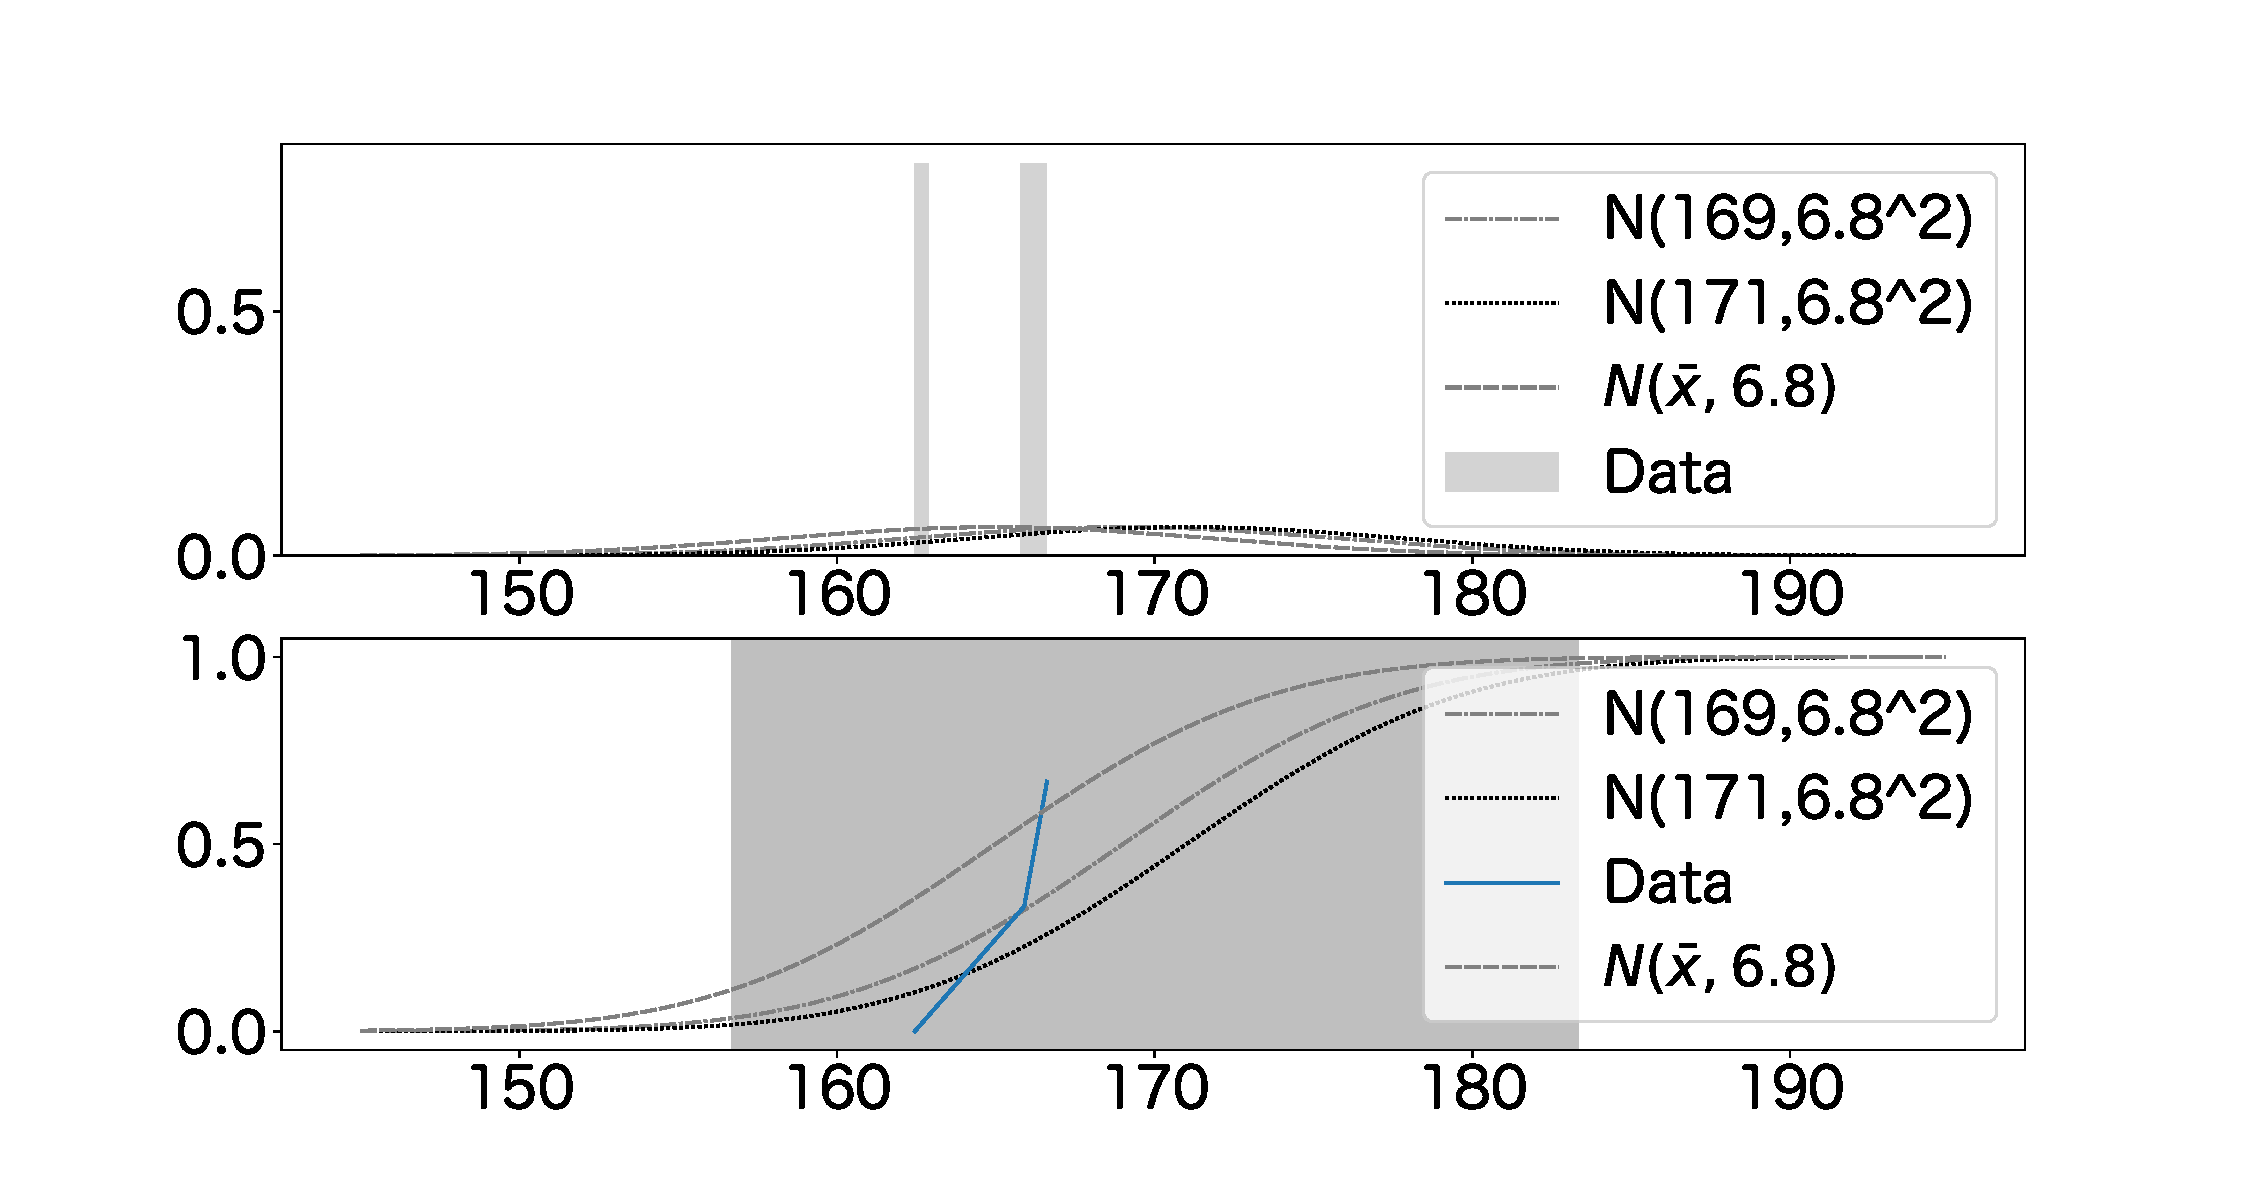
\includegraphics[width=15cm]{../markdown/section1/maximum_likelihood_3.pdf}
        \caption{$N(170,6.8^2)$からサンプルサイズ$3$の標本を得たときの分布。その最尤推定量により求められる分布関数。$N(168,6.8^2),N(171,6.8^2)$の分布関数を示す}
        \label{fig:maximum_likelihood_0}
    \end{center}
\end{figure}

\subsection{全然違うはなんとなくわかる}
図\ref{fig:maximum_likelihood_false_3},\ref{fig:maximum_likelihood_false_30}は、$N(170,6.8^2)$からサンプリングしたデータの度数分布と、その確率密度関数とは著しく異なる確率密度関数を表示したものです。

\begin{figure}
    \begin{center}
        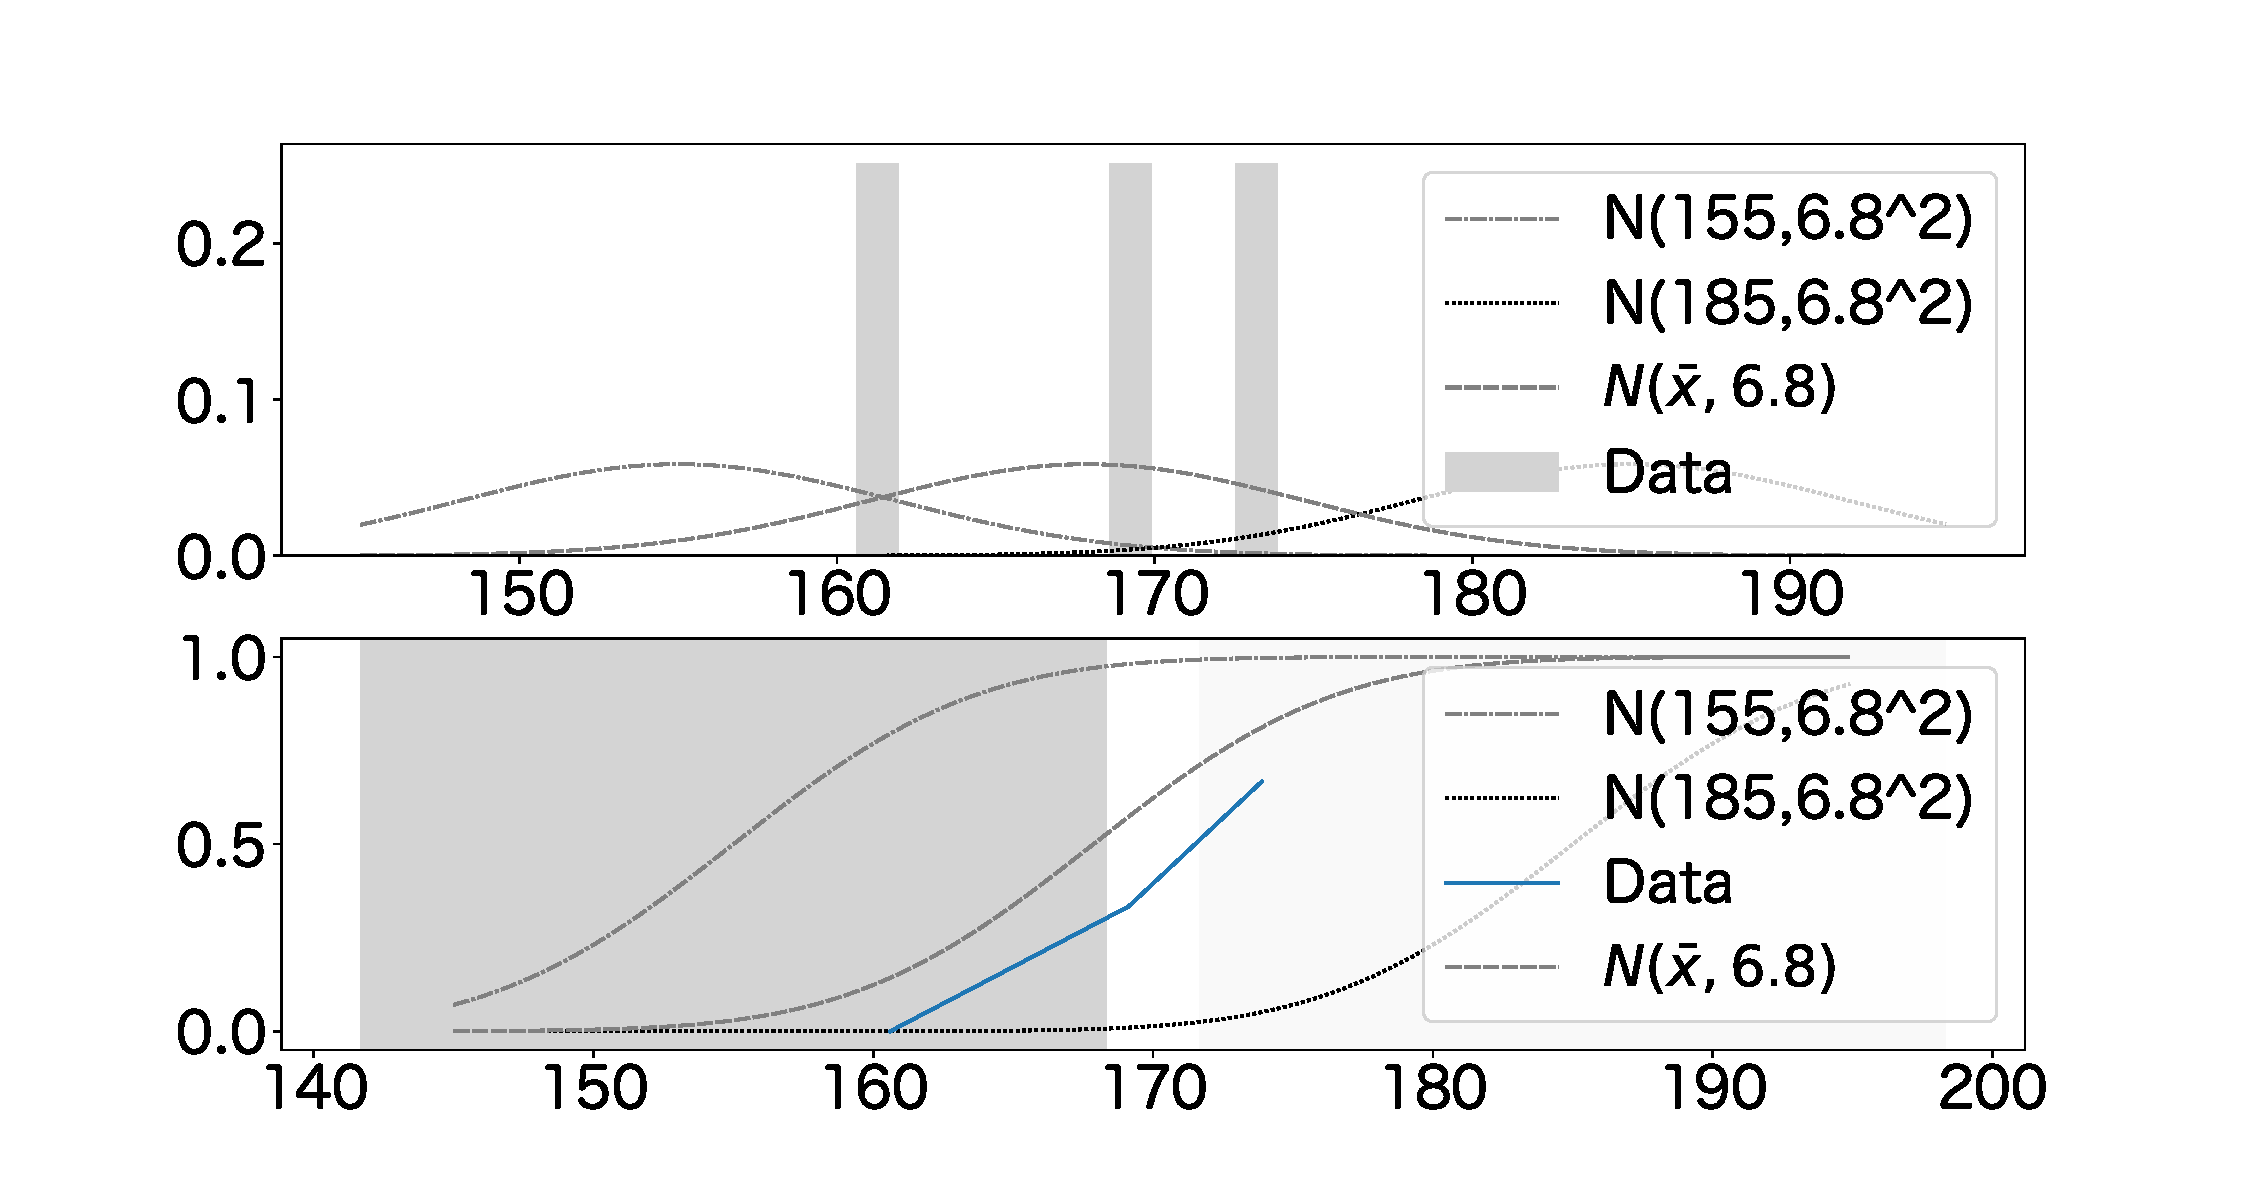
\includegraphics[width=15cm]{../markdown/section1/maximum_likelihood_false_3.pdf}
        \caption{$N(170,6.8^2)$からサンプルサイズ$3$の標本を得たときの分布。その最尤推定量により求められる分布関数。$N(168,6.8^2),N(171,6.8^2)$の分布関数を示す}
        \label{fig:maximum_likelihood_false_3}
    \end{center}
\end{figure}

\begin{figure}
    \begin{center}
        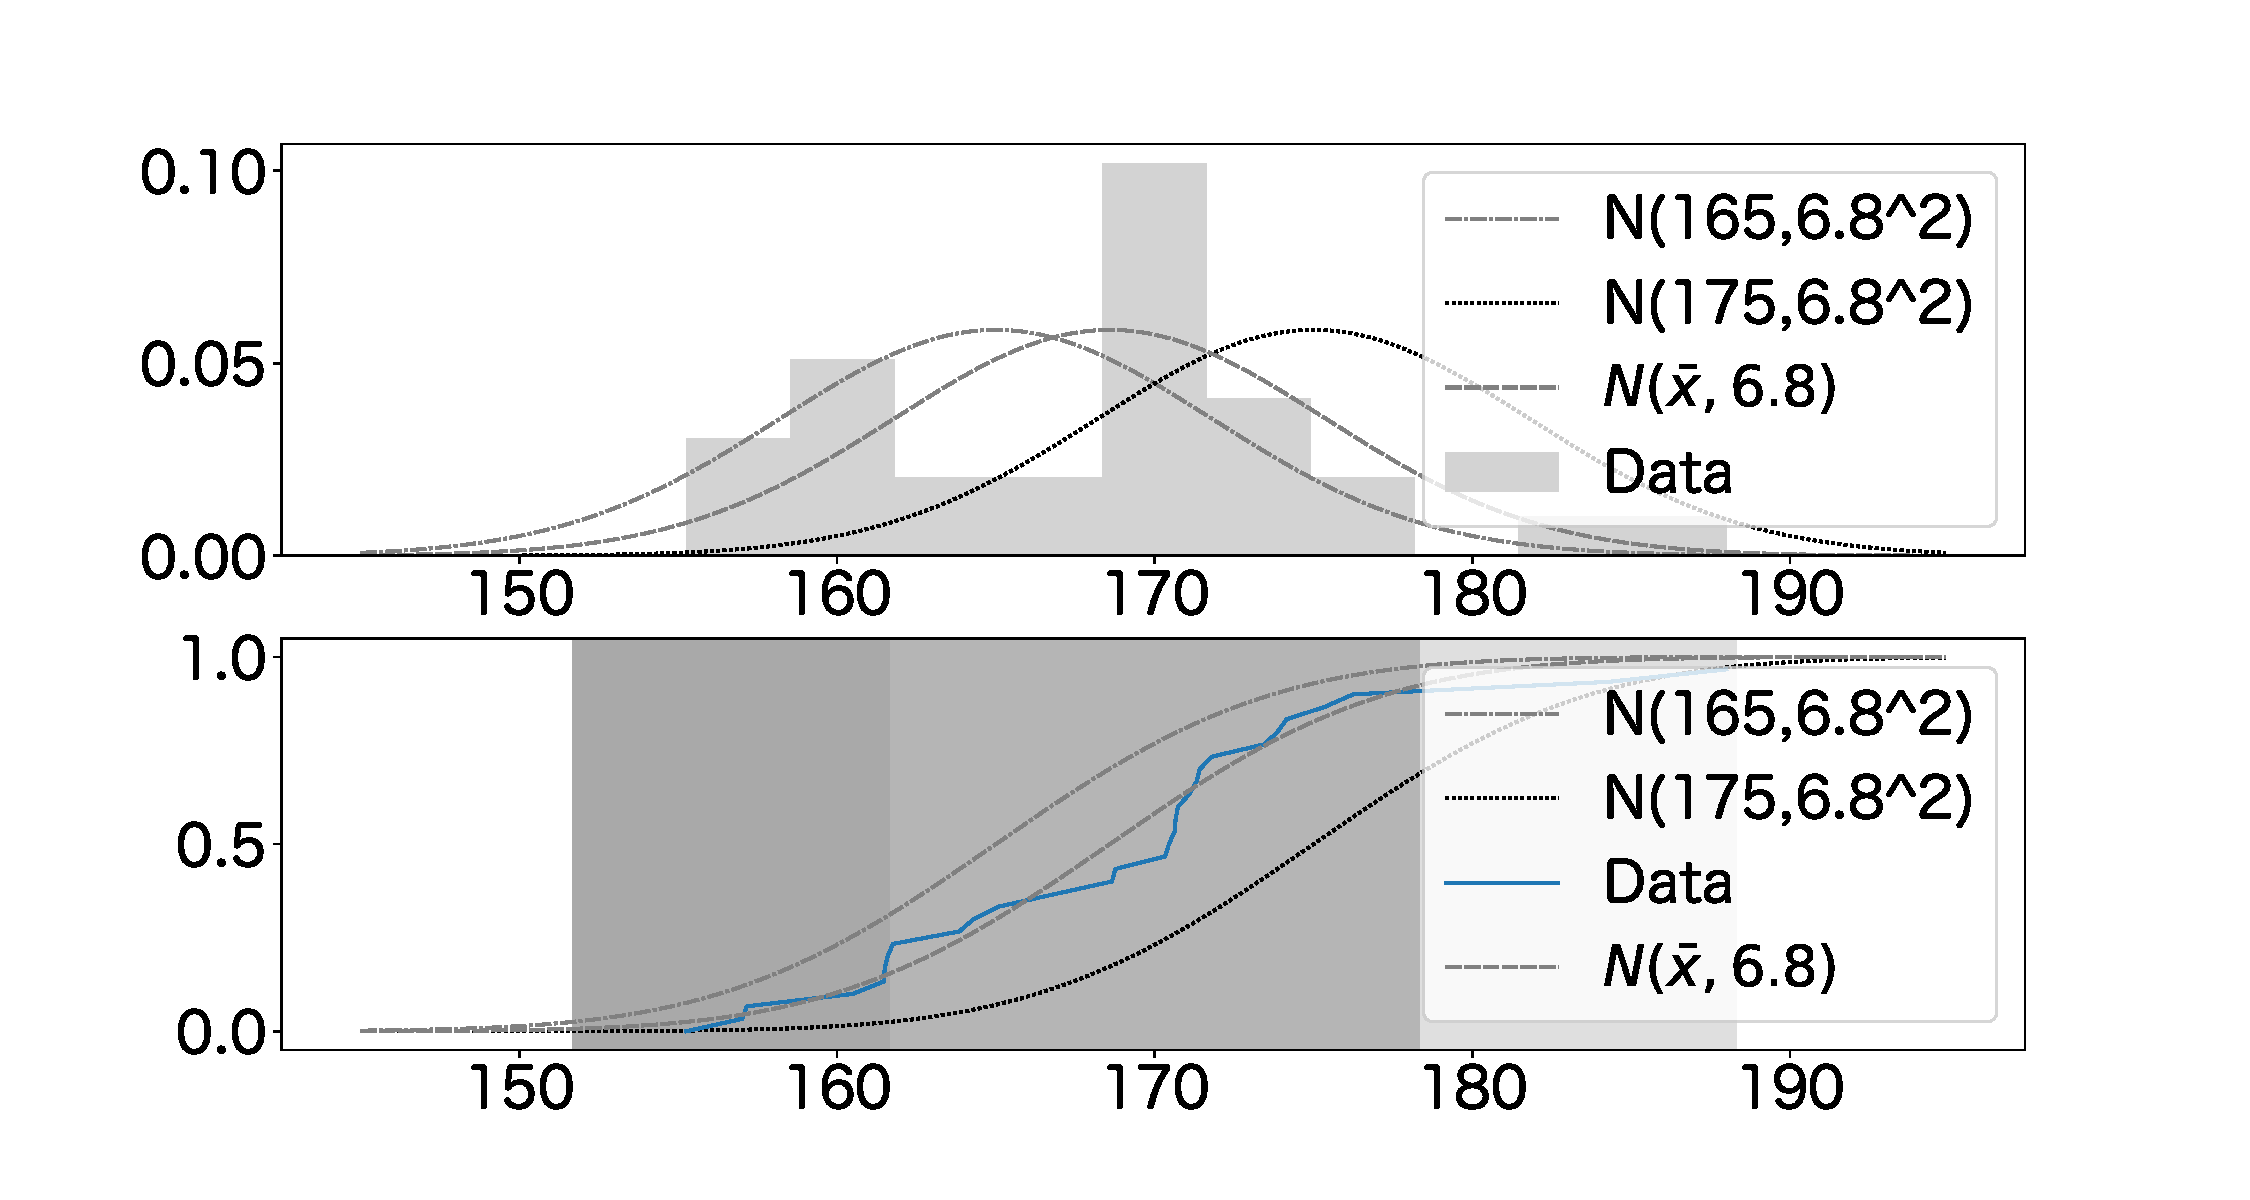
\includegraphics[width=15cm]{../markdown/section1/maximum_likelihood_false_30.pdf}
        \caption{$N(170,6.8^2)$からサンプルサイズ$3$の標本を得たときの分布。その最尤推定量により求められる分布関数。$N(168,6.8^2),N(171,6.8^2)$の分布関数を示す}
        \label{fig:maximum_likelihood_false_30}
    \end{center}
\end{figure}

\clearpage
\subsection{再生性を使う}
\subsubsection{$(\star)$ $N(\mu,\sigma^2)$に従う確率変数であることを判定できるか}
$N(0,1)$に従う確率$x_1,x_2,\cdots,x_n$から計算した統計量、$z=\frac{\bar{X}-0}{\sqrt{\frac{1}{n}}}$は、$N(0,1)$に従い、$z$が$95\%$の確率で見つかる範囲は$[-1.96,1.96]$である。
同様に、$y_1,y_2,\cdots,y_n \sim N(1.96,1)$であるならば、$z=\frac{\bar{Y}-1.96}{\sqrt{\frac{1}{n}}}$は、$N(0,1)$に従う。

確率変数から、特定の母数を持つ正規分布に従わないことを示すことはできるだろうか。
具体的な問題設定として、
$y_1,y_2,\cdots,y_n$を正規分布に従う確率変数とする。そのとき、$y_1,y_2,\cdots,y_n$が$N(\mu,\sigma^2)$に従わないことを判断する良い方法はどのようなものだろうか。

ここで、$y_1,y_2,\cdots,y_m \sim N(1.96,1)$にもかかわらず、$N(0,1)$に従うと推測した場合、$z=\frac{\bar{Y}-0}{\frac{1}{\sqrt{n}}} \sim N(0,1)$であると考えられる。
$z$の分子の$\mu$が$0$になっていることに注意が必要である。
実際に、$y_1,y_2,\cdots y_{100}$を$N(1.96,1)$からサンプリングした標本を$100$個作ってみると、およそ$19$を中心に分布することがわかる。
このことは、$y_1,y_2,\cdots,y_m\sim N(0,1)$であるならば、$z$は、$[-1.96,1.96]$の間で$95\%$の確率で入るので、この推測が間違いであることが推測される。
以上の考察から、$y_1,y_2\cdots,y_n\sim N(0,1)$ではないと判断する。

\begin{figure}
    \begin{center}
        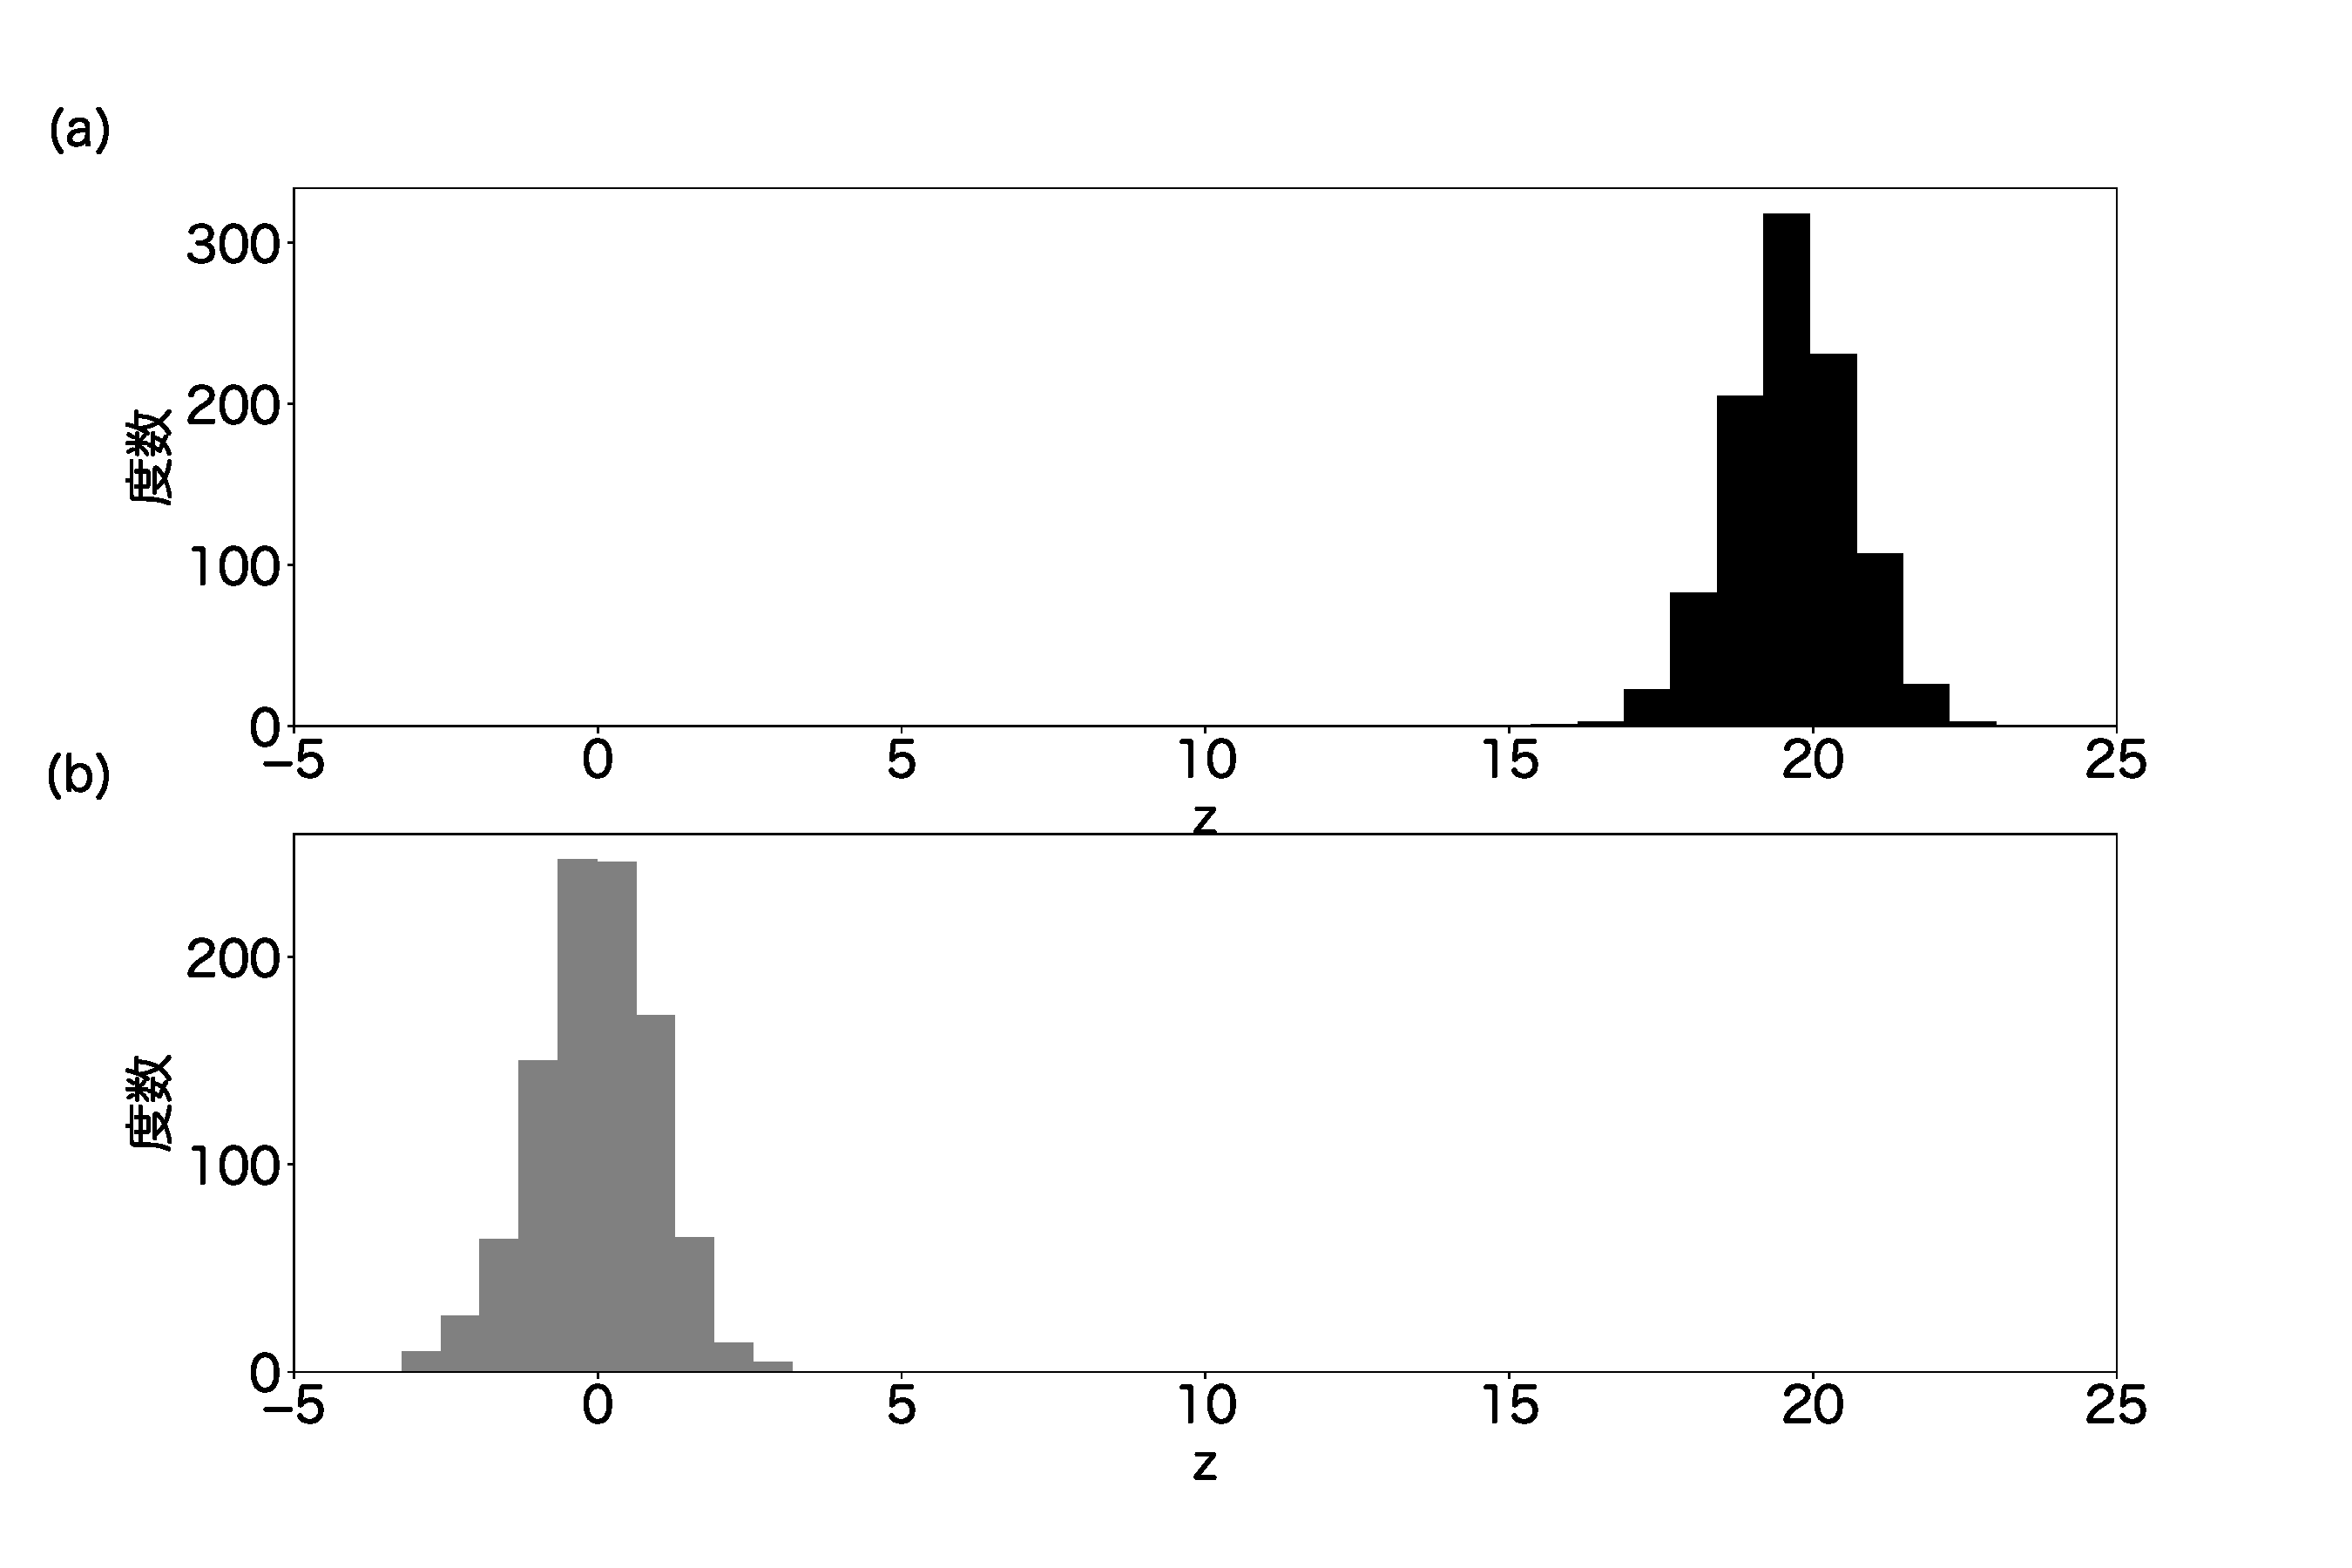
\includegraphics[width=15cm]{../markdown/section1/normal_distribution_test.pdf}
        \caption{(a)$N(1.96)$に従う確率変数を100個サンプリングし、その標本を1000個集めたときの$z=\sqrt{100}(\bar{X}-0)$のヒストグラム (b)$N(0,1)$に従う確率変数を100個サンプリングし、その標本を1000個集めたときの$z=\sqrt{100}(\bar{X}-0)$値のヒストグラム}
    \end{center}
\end{figure}


もう一つ例を挙げる。
$y_1,y_2,\cdots,y_n \sim N(170,5.8)$とする。このとき、この標本が$N(168,5.8)$によりサンプリングされたものではなくことを示すことはできるだろうか。
$z=\sqrt{n}\frac{\bar{y}-168}{\sigma}$を計算すればよい。
図には、$N(170,5.8)$に従う確率変数を100個サンプリングし、その標本を1000個集め、ヒストグラムを描いた。
これをみると、$0.5$を中心に分布が広がることがわかる。$z=\frac{\bar{X}-168}{\sqrt{\frac{5.8}{n}}}\sim N(0,1)$であるはずである。
複数回、標本を得た場合でも、$z$が$[-1.96,1.96]$の範囲に収まっている。このことは、$N(168,5.8)$ではないと判断できないことを示唆している。


\begin{figure}
    \begin{center}
        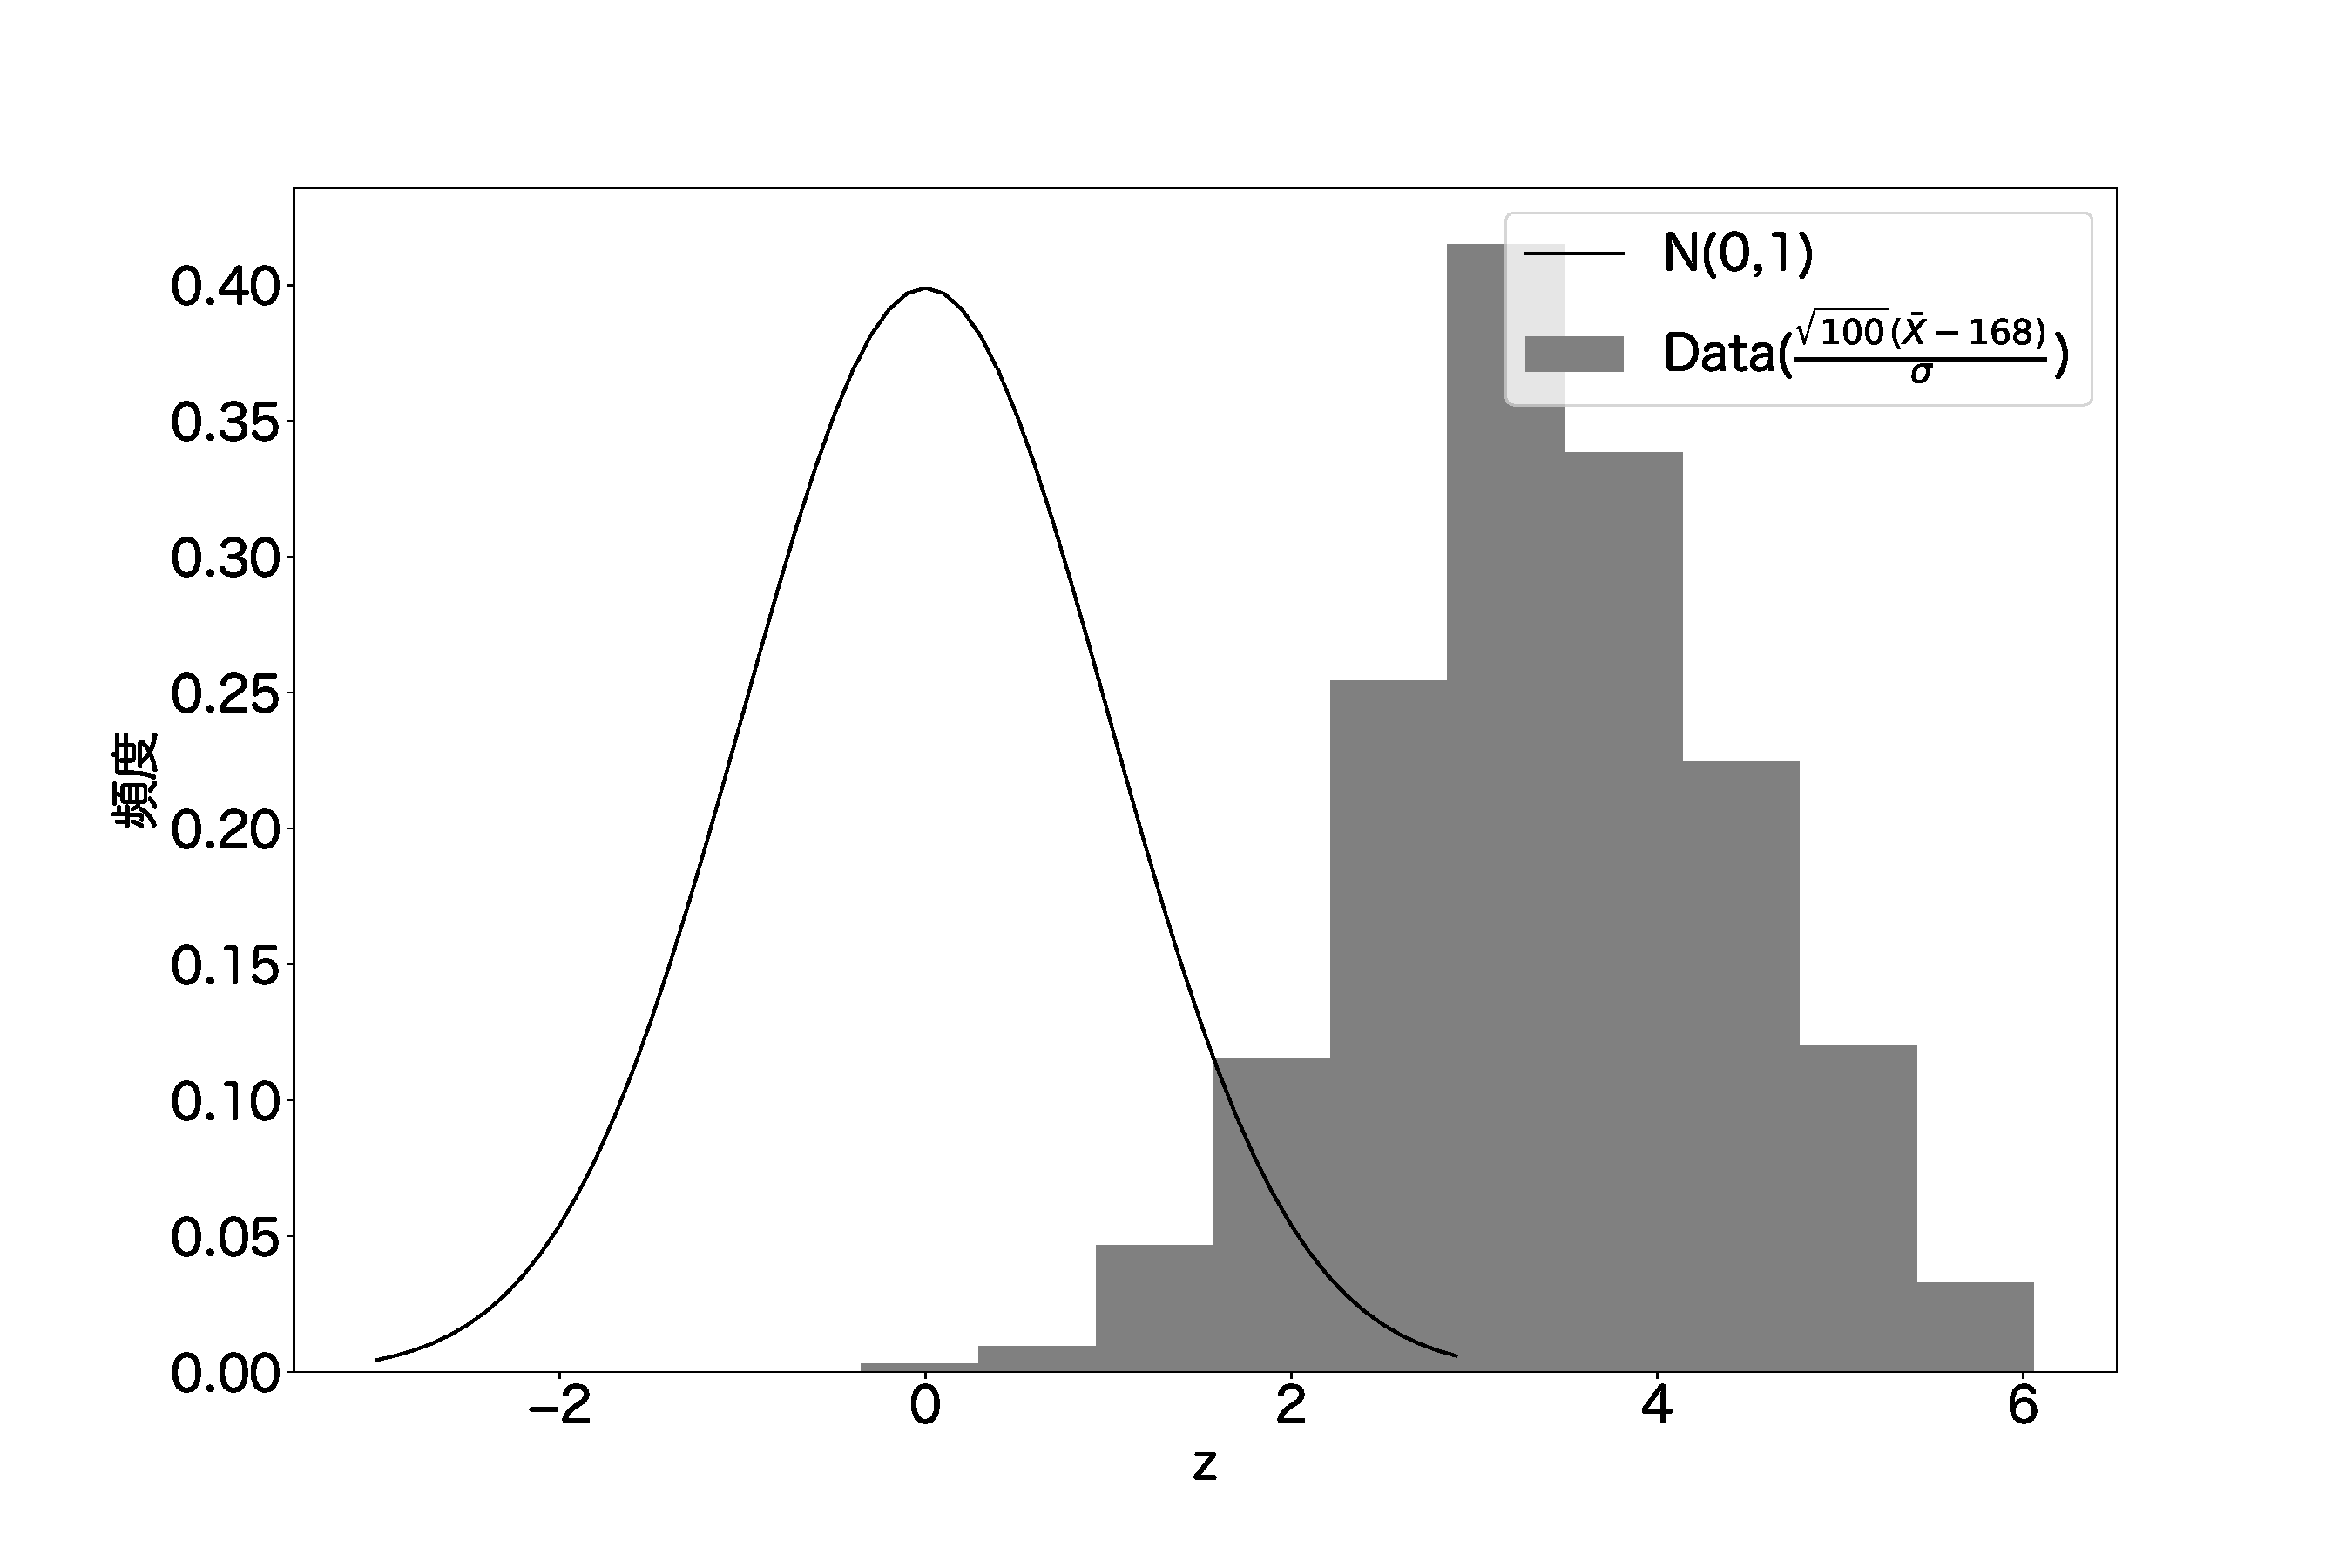
\includegraphics[width=15cm]{../markdown/section1/normal_distribution_test2.pdf}
        \caption{$N(170,5.8)$に従う確率変数を100個サンプリングし、その標本を1000個集めたときの$z=\sqrt{100}(\bar{X}-168)$のヒストグラム}
    \end{center}
\end{figure}


ある正規分布に従う確率変数$x_1,x_2,\cdots,x_n$が母数の異なる正規分布で得られる確率も計算できる。具体的には、$x_1,x_2,\cdots,x_n\sim N(\mu,\sigma^2)$とし、これが$N(\mu_1,\sigma_1^2)$で得られるとすると、そのときの統計量は、$z=\frac{\bar{x}-\mu_1}{\frac{\sigma_1}{n}}$である。この$z$は、$N(0,1)$に従うと考えられるので、$\phi(|z|>Z)$となる確率を計算すれば良い。

\begin{theo}
    確率変数$x_1,x_2,\cdots,x_n \sim N(\mu,\sigma^2)$ならば、$z=\frac{\bar{X}-\mu}{\sqrt{\frac{\sigma}{n}}} \sim N(0,1)$である。
    一方で、確率変数$x_1,x_2,\cdots,x_n \sim N(\mu,\sigma^2)$とする。$N(\mu_1,\sigma_1^2)$は正規分布とする。ただし、$\mu\neq \mu_1, \sigma =\sigma_1$このとき、$z=\frac{\bar{X}-\mu_1}{\sqrt{\frac{\sigma_1}{n}}} \sim N(0,1)$ではない。
\end{theo}
$\mu$と$ \mu_1$が極めて近い値のとき、$z=\frac{\bar{X}-\mu_1}{\sqrt{\frac{\sigma_1}{n}}} $も$N(0,1)$におけるよくある値になる言い換えれば、$\phi(|z|>Z)$は十分大きい。
一方で、$\mu$と$ \mu_1$が離れた値を取ると、$\phi(|z|>Z)$は小さな値になる。


\subsubsection{$(\star)$ $Exp(\lambda)$に従う確率変数であることを判定できるか}
$x_1,x_2,\cdots,x_n \sim Exp(\lambda)$であるとき、$n\bar{x}\sim Ga(n,\frac{1}{\lambda})$である。
母数不明の指数分布に従う確率変数が、$x_1,x_2,\cdots,x_n \sim Exp(\lambda)$と仮定したとき、$n\bar{x}\sim Ga(n,\frac{1}{\lambda})$でないならば、$x_1,x_2,\cdots,x_n \sim Exp(\lambda)$ではないと判断できるだろうか。シミュレーションによって確認してみよう。

この論法は、母数が不明の指数分布に従う確率変数を得たとき、その指数分布の母数が特定の値ではないことを示すためにこの論法を利用する。ここでは、母数が$\lambda=1,2,5,10,100$からサンプルサイズ4の標本を$1000$生成し、それら標本の統計量$n\bar{X}$のヒストグラムと、ガンマ関数$Ga(100,1)$の確率密度関数を比較する。

\begin{figure}
    \centering
    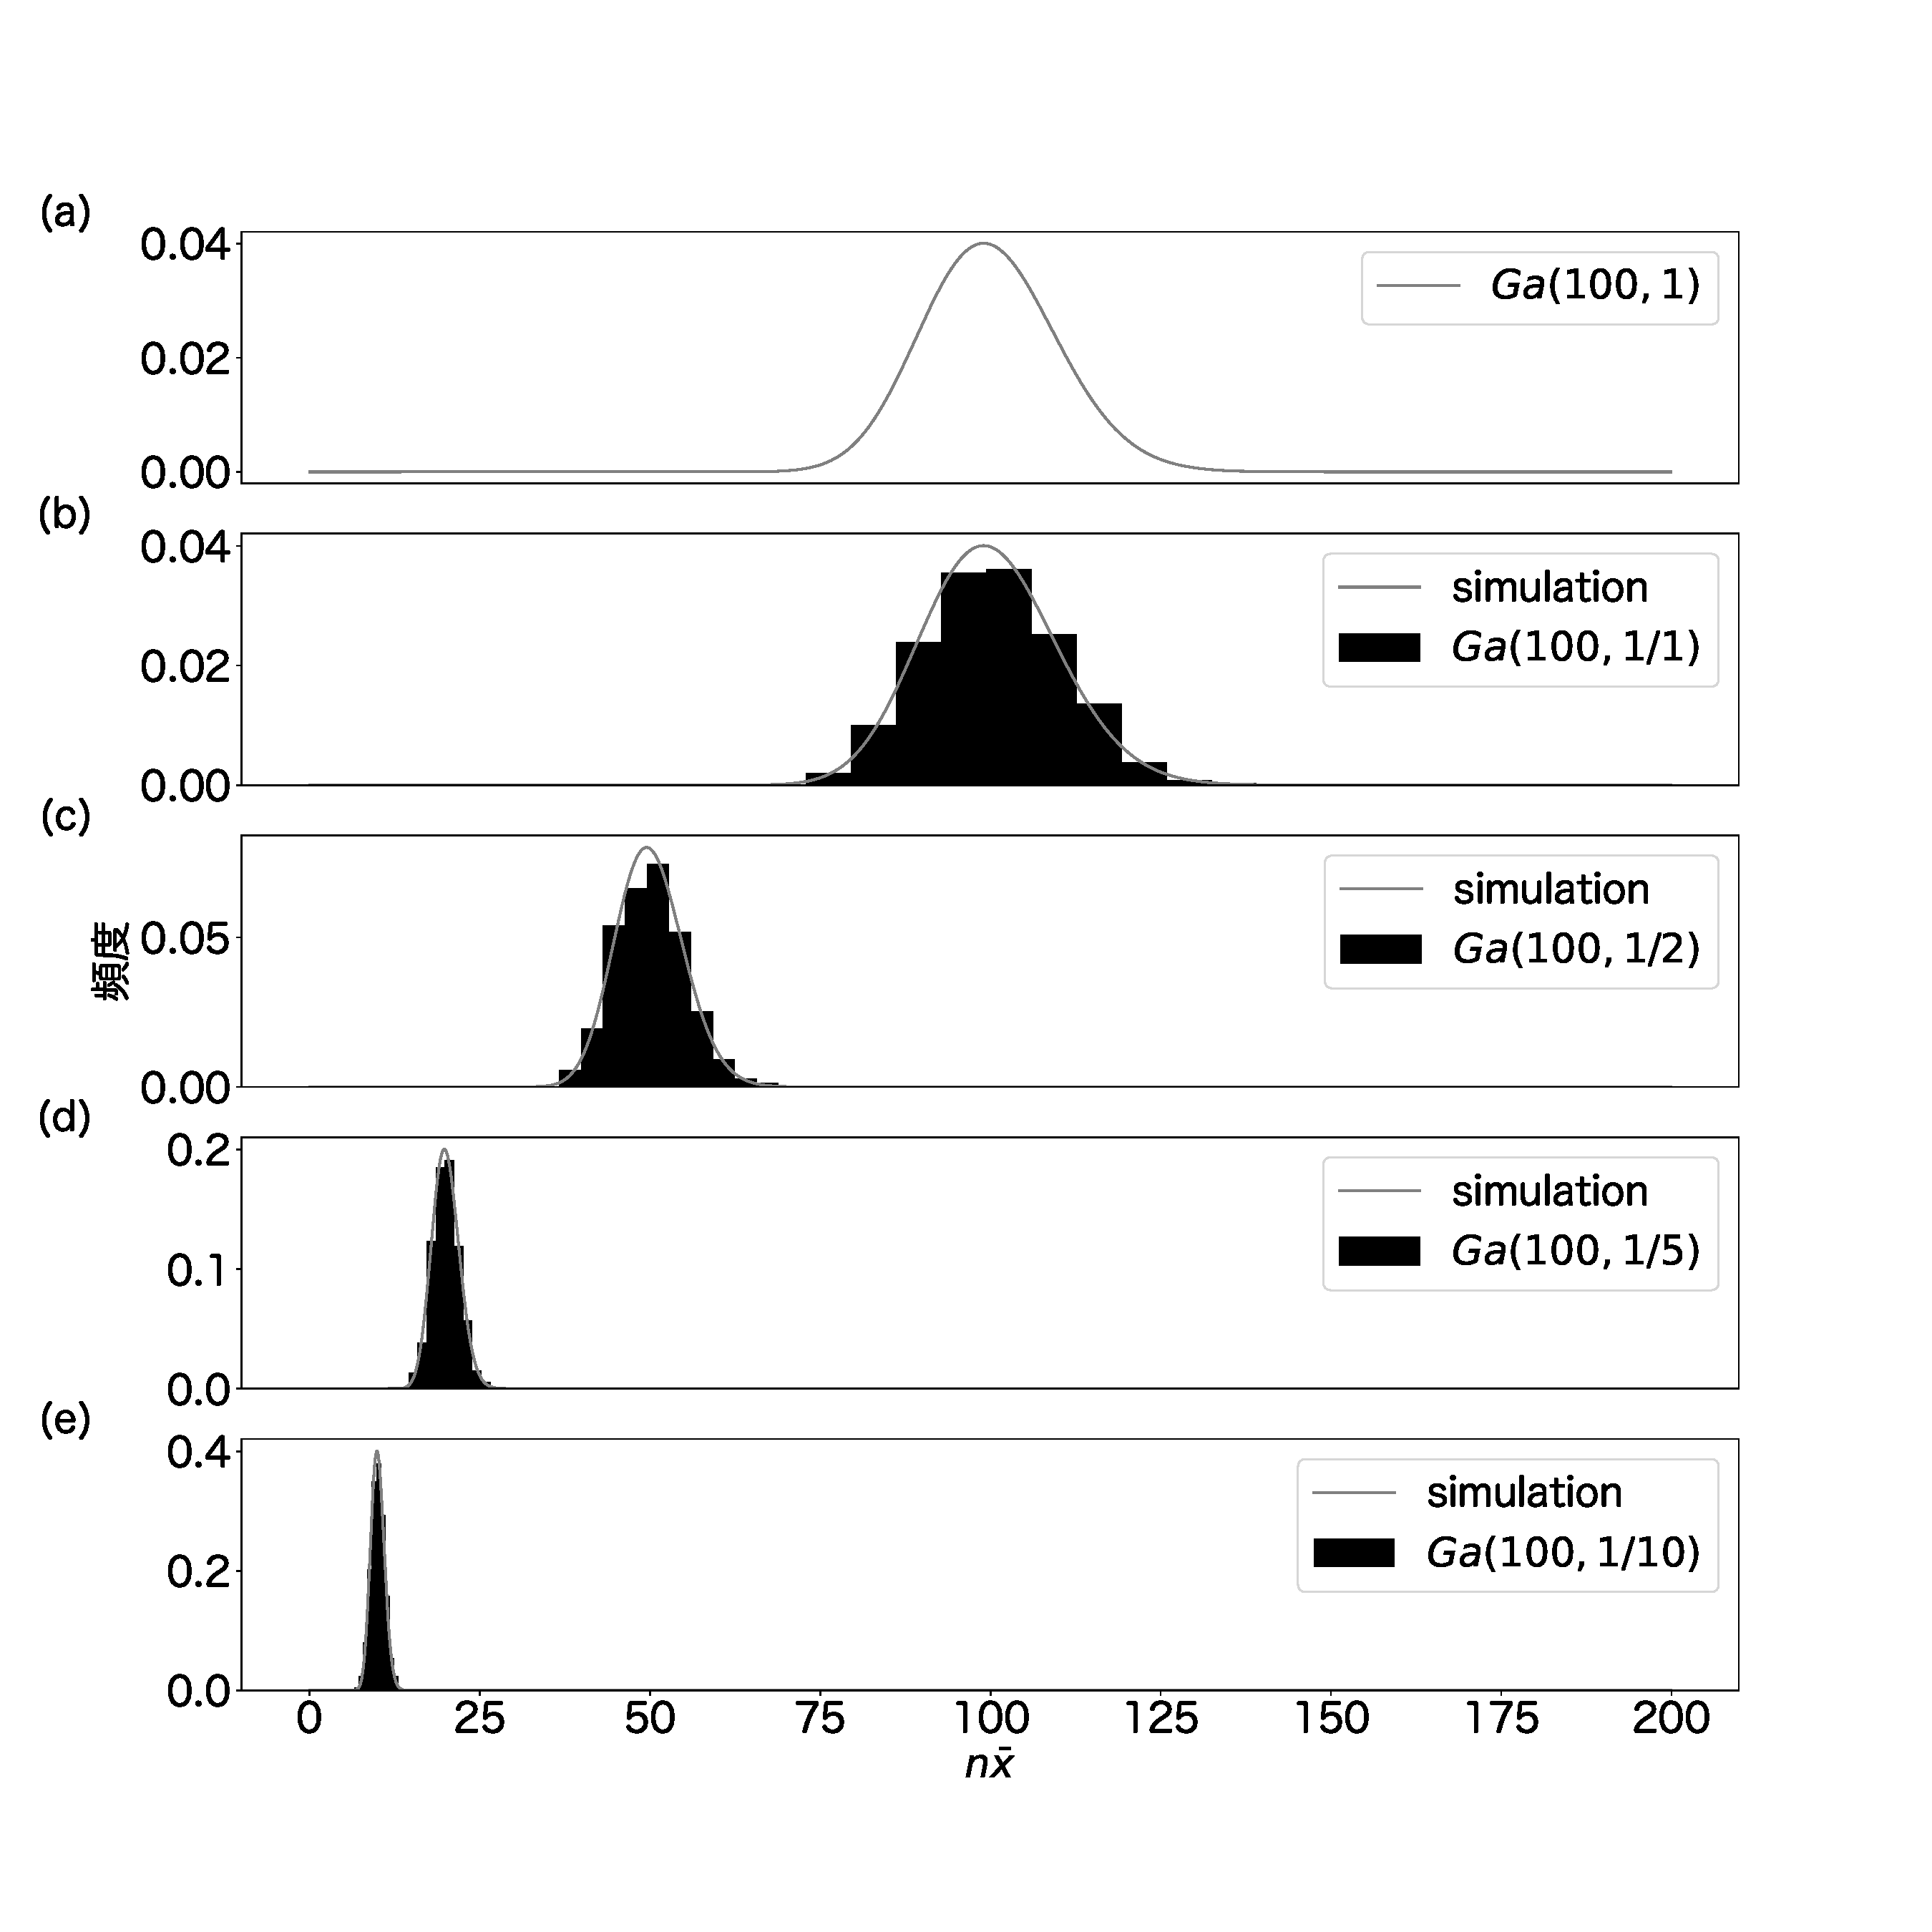
\includegraphics[width=15cm]{../markdown/section1/Exp_Gamma_simulation.pdf}
    \caption{(a)$Ga(10,1)$の確率密度関数。(b-e)指数分布からサンプルサイズ$4$の標本を$1000$回生成し、その統計量$n\bar{x}$のヒストグラム}
    \label{fig:exp_gamma_simulation}
\end{figure}

図\ref{fig:exp_gamma_simulation}(a)は、指数分布$Exp(\lambda=1)$の確率密度関数を示している。
図\ref{fig:exp_gamma_simulation}b-eは、シミュレーションの結果を示している。
図\ref{fig:exp_gamma_simulation}(b)には、指数分布$Exp(1)$に従う確率変数の統計量$n\bar{x}$が確かに、$Ga(100,1)$に従うことが確かめれる。
図\ref{fig:exp_gamma_simulation}(c-e)では、指数分布の$\lambda$が$1/2,1/5,1/10$のときの統計量のヒストグラムである。これらと、図\ref{fig:exp_gamma_simulation}(a)を比較すると、分布が異なっているので、確かに、$Ga(100,1)$には従わないことがわかる。



\subsection{問題点}
aa


\clearpage
\section{身長を予測する統計モデル}
\subsection{正規分布を組み入れた統計モデル}
日本人の$17$歳男性の身長を予測する統計モデルを構築していきましょう。この統計モデルは次の1-3から構成されます。
\begin{quote}
    \begin{enumerate}[(1)]
    \item 独立同分布
    \item その分布は、正規分布
    \item 正規分布の母数(平均と分散)はそれぞれ$\mu,\sigma^2=5.7$である。
    \end{enumerate}
\end{quote}

$\mu$を変数としたこの統計モデルを$M(\mu)$とします\footnote{三番目の仮説のみを統計モデルと主張する流派もある\cite{塩見_正衛2021}。数理統計学の知識を使うには、少なくとも$3$つので一つの統計モデルであると私は考えている}。
およその平均値は日本にいれば母集団の分布をなんとなく知っているので、$\mu=171.1\mathrm{cm}$であると言えます。
一方で、分散をどの程度にするかは、母集団のばらつき具合を意識して知ることが少ないので、設定しずらいところです。
今回は、カンで$5.7$としました\footnote{もちろんかんではなく、統計データを覗き見した。分散を経験で推定できる人はすごいと思います。}。
$\mu=171.1$としたときの統計モデル$M(171.1)$を使って、身長に関する推測を行ってみます。

\paragraph{ $\circ\circ \mathrm{cm}$以下、$\diamond\diamond \mathrm{cm}$以上の人がどれくらい含まれるか}
まず、母集団に$180cm$以下、$180cm$以上の人がどれくらい含まれているのかを推測してみます。正規分布関数を使い、$P(x>180)$を計算します。

\begin{lstlisting}
norm.cdf(180,171.1,5.7)
1-norm.cdf(180,171.1,5.7)
\end{lstlisting}
結果、 $P(x<180)=0.940$、$P(x>180)=0.059$ということが分かります。
このことから、母集団から100人無作為抽出を行うと内$5$人程度は$180cm$以上であることが推測されます。

もう一つ、$160cm$以下の人がどれくらい含まれるかを調べてみます。

\begin{lstlisting}
norm.cdf(160,171.1,5.7)
1-norm.cdf(160,171.1,5.7)
\end{lstlisting}
結果、$P(x<160)=0.059$、$P(x>160)=0.940$と推測されました。

$P(x<160)$と$P(x>180)$が極めて近い値であることがわかります。
正規分布は、母平均$\mu=171.1$を中心に、対称にデータが分布するので、$171.1$からおよそ$10cm$離れた$160cm$と$180cm$の人ではおよそ同じくらいの出現頻度であると推定されます。


    
\paragraph{擬似的に無作為を行うサンプリング}
$10$人分のデータをサンプリングしてみると、以下の数値が得られます。
$10$人を母集団から無作為抽出すると、およそこのようなデータが得られることがあると推測できる。

\begin{lstlisting}
168.575192 164.5988088 162.7027275 163.9689649 169.8187076 174.8851702 172.767133 165.0665034 175.7370453 163.0385381
\end{lstlisting}



\subsection{データとの比較}
統計モデル$M(171.1)$を使った推測は、的外れなものになっていないかを確認してみます。
17歳男性の身長を無作為抽出してサンプルサイズを稼ぐのには時間とお金がかかりすぎますので、公開されているデータ\footnote{ \url{https://www.e-stat.go.jp/dbview?sid=0003107092} }\footnote{\url{https://www.e-stat.go.jp/dbview?sid=0003037791}}を使ってみます。
このデータは文部科学大臣があらかじめ指定した1410校の高校に在籍する生徒を対象にしています。

\begin{figure}
\begin{center}
    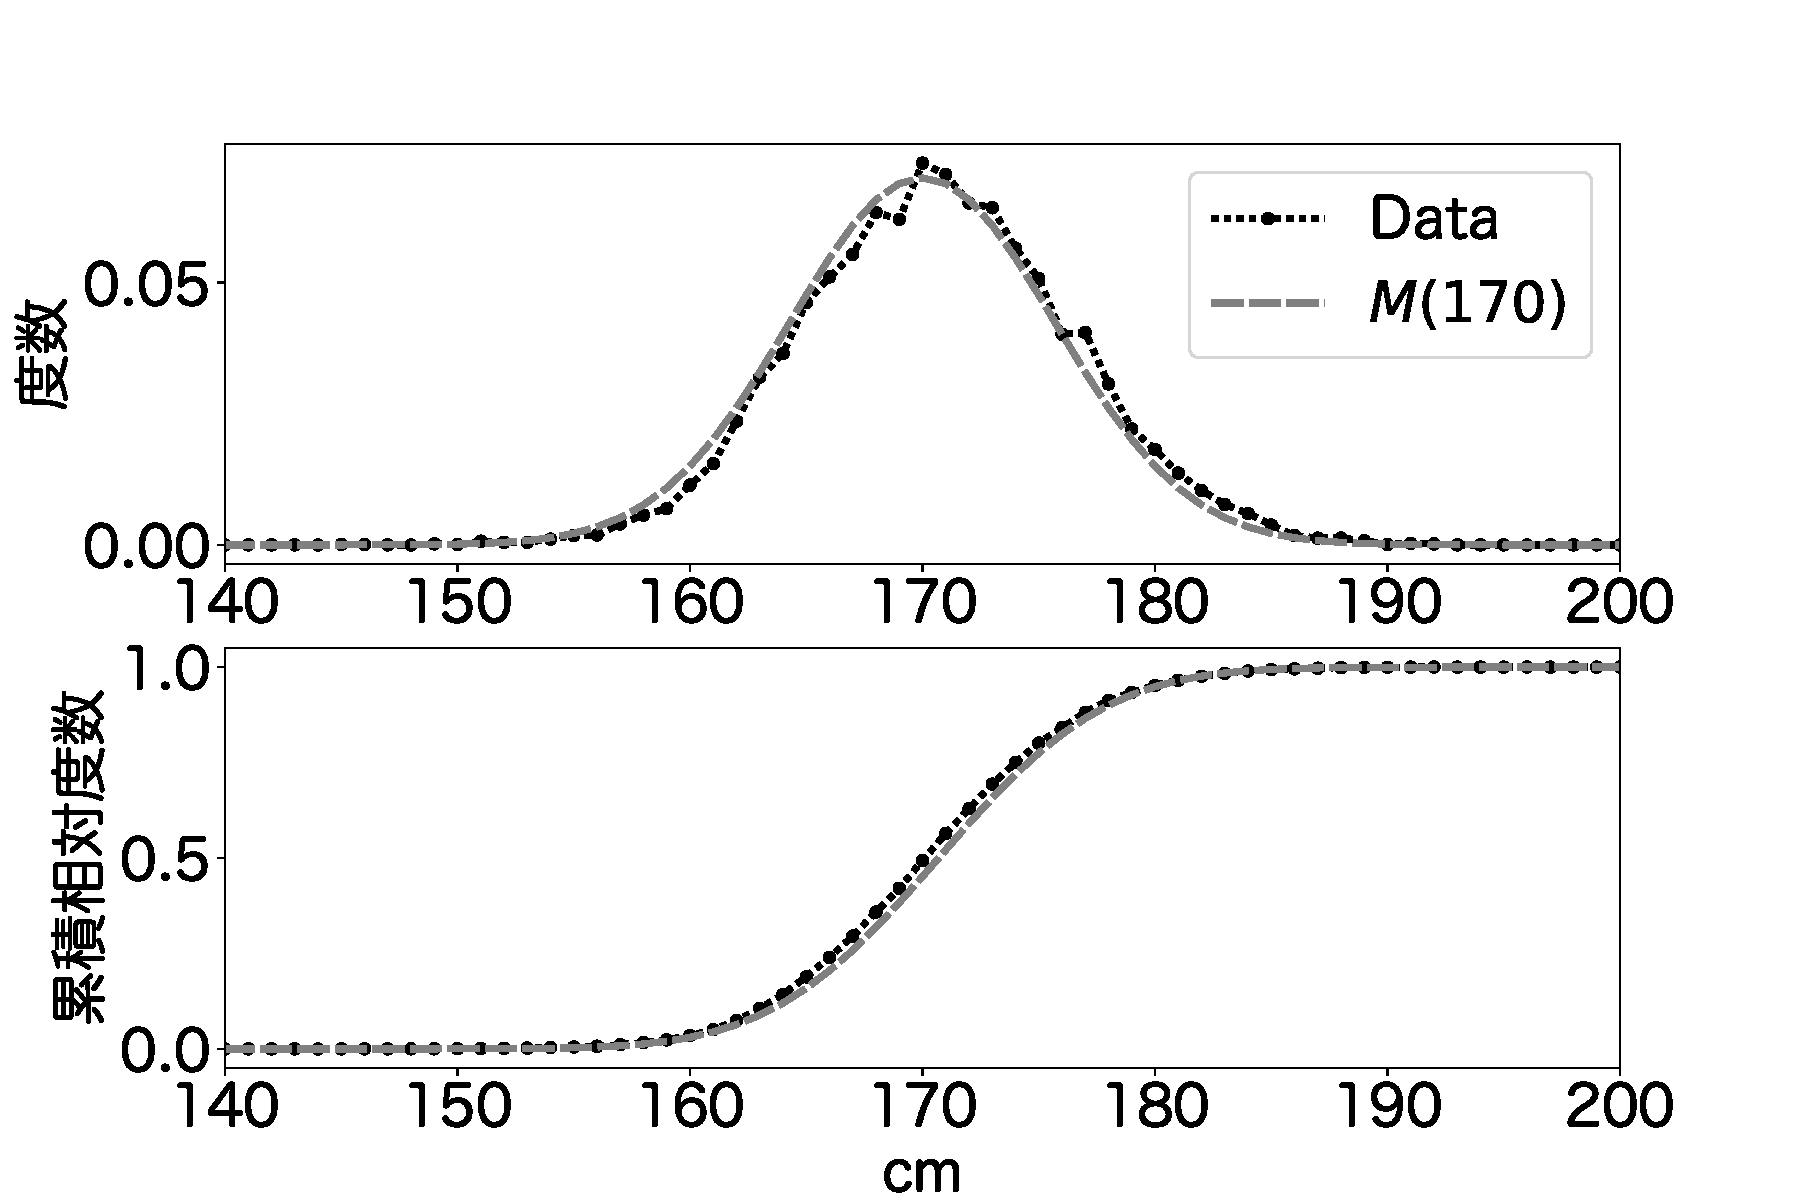
\includegraphics[width=15cm]{../markdown/section1/cm_data.pdf}
    \caption{17歳の男性から無作為抽出したデータ。上は、データと統計モデル$M(170)$の度数。下は、データと統計モデル$M(170)$の累積相対度数}
    \label{fig:real_height_men}
\end{center}
\end{figure}


\paragraph{$170cm$を少し超えた人が多いのは、不正(無作為抽出の手順に異常)があったから?}
\begin{quotation}
    「生物学上、グラフは曲線になっていなければならないが、169cmの部分はへこんでいる。これは先生や生徒による四捨五入で生まれるサバ読みの結果。身長が170cmなのか169cmなのかで気持ち的に違ってきますからね」と話すと、食料自給率や犯罪発生件数とは異なる微笑ましいサバ読みのトリックに、出演者一同、笑みを浮かべていた。\footnote{国民を欺く“統計のウソ” 知らないと怖い“統計トリック”を専門家が解説
    \url{https://times.abema.tv/articles/-/5640846} 2022/04/30確認}
\end{quotation}

このように、データが統計モデルに一致しないことから、データに不正な操作が加わっているという推測がされることがある。議論となっている身長のデータを観察してみる。
図\ref{fig:real_height_men}上を見ると、確かに、$170$を超えたあたりの度数は、$169$の度数よりも多い感じがする。
また、$170cm$以下のデータは統計モデルの度数よりも低く、$17cm$以上のデータは統計モデルの度数よりも大きい。一方で、図\ref{fig:real_height_men}下の累積相対度数を見ると、そのような変異があるようには見ることができない。このようなデータと統計モデルの相違の原因は、データを無作為抽出するときの不正な操作により生じたと断言できるのだろうか。

データとモデルの相違が、恣意的な操作以外からも生じることを確認する。
具体的には、データを統計モデルからサンプリングし、そのデータが統計モデルと一致するかを観察してみる(図\ref{fig:simulation_height_men})。図を見るとわかるように、サンプリングを行った場合、$168cm$付近で、度数が曲線よりも上にくる部分がある。また、$170cm$より小さいところでは、統計モデルよりもデータの度数が上にあり、$170cm$より大きなところでは、統計モデルより、データの度数が下にある。このように、統計モデルによりサンプリングし、統計モデルとサンプリングデータを比較した場合でも、ズレが生じる。単純なズレだけを見たとしても、それが不正なのかは結論をつけることは難しい。

一方で、次のような経験があれば、不正を見つけることも可能だろう。恣意的な操作を一切介入させない、かつ、無作為にデータを取得したときに、データが統計モデルに一致していると言う経験である。
この経験があれば、同じ計測方法・同じ生徒なのに、データが統計モデルに一致しないのは、不正な操作が加わったことが疑える。

きっちりとデータを収集する手順が満たされていないのではないかと疑うことはした方が良い。
例えば、髪の毛や靴などを履いる人がそうではない人と同じように計測をされると、平均値が大きくなる。身長の低い生徒に対してその傾向が高ければデータには歪みが生じやすくなる。計測を行なった先生方の疲れなども考慮すれば、恣意的な操作が一切無いとは言い難い。
%この知識がない場合、不正な処理が加わったことを断言することはやはり極めて難しい。

データの無作為抽出には多大な労力がかかっている。誰かがどこかで腰を痛めながら高校生の身長を測る仕事をしていることは心に留めておくべきで、不正があったと主張するのは、彼らの仕事を低く評価しすぎではないだろうか。おそらく先生たちは、正確に計測できるように正確に手順を満たすように計測しているはずである。
不正を疑うならば、それなりに確証できる証拠を提示すべきである。具体的には、自分が手順を守って計測したデータと、先生が測ったときのデータにおいて、それらの間の差を示すべきである。

 \begin{figure}
\begin{center}
    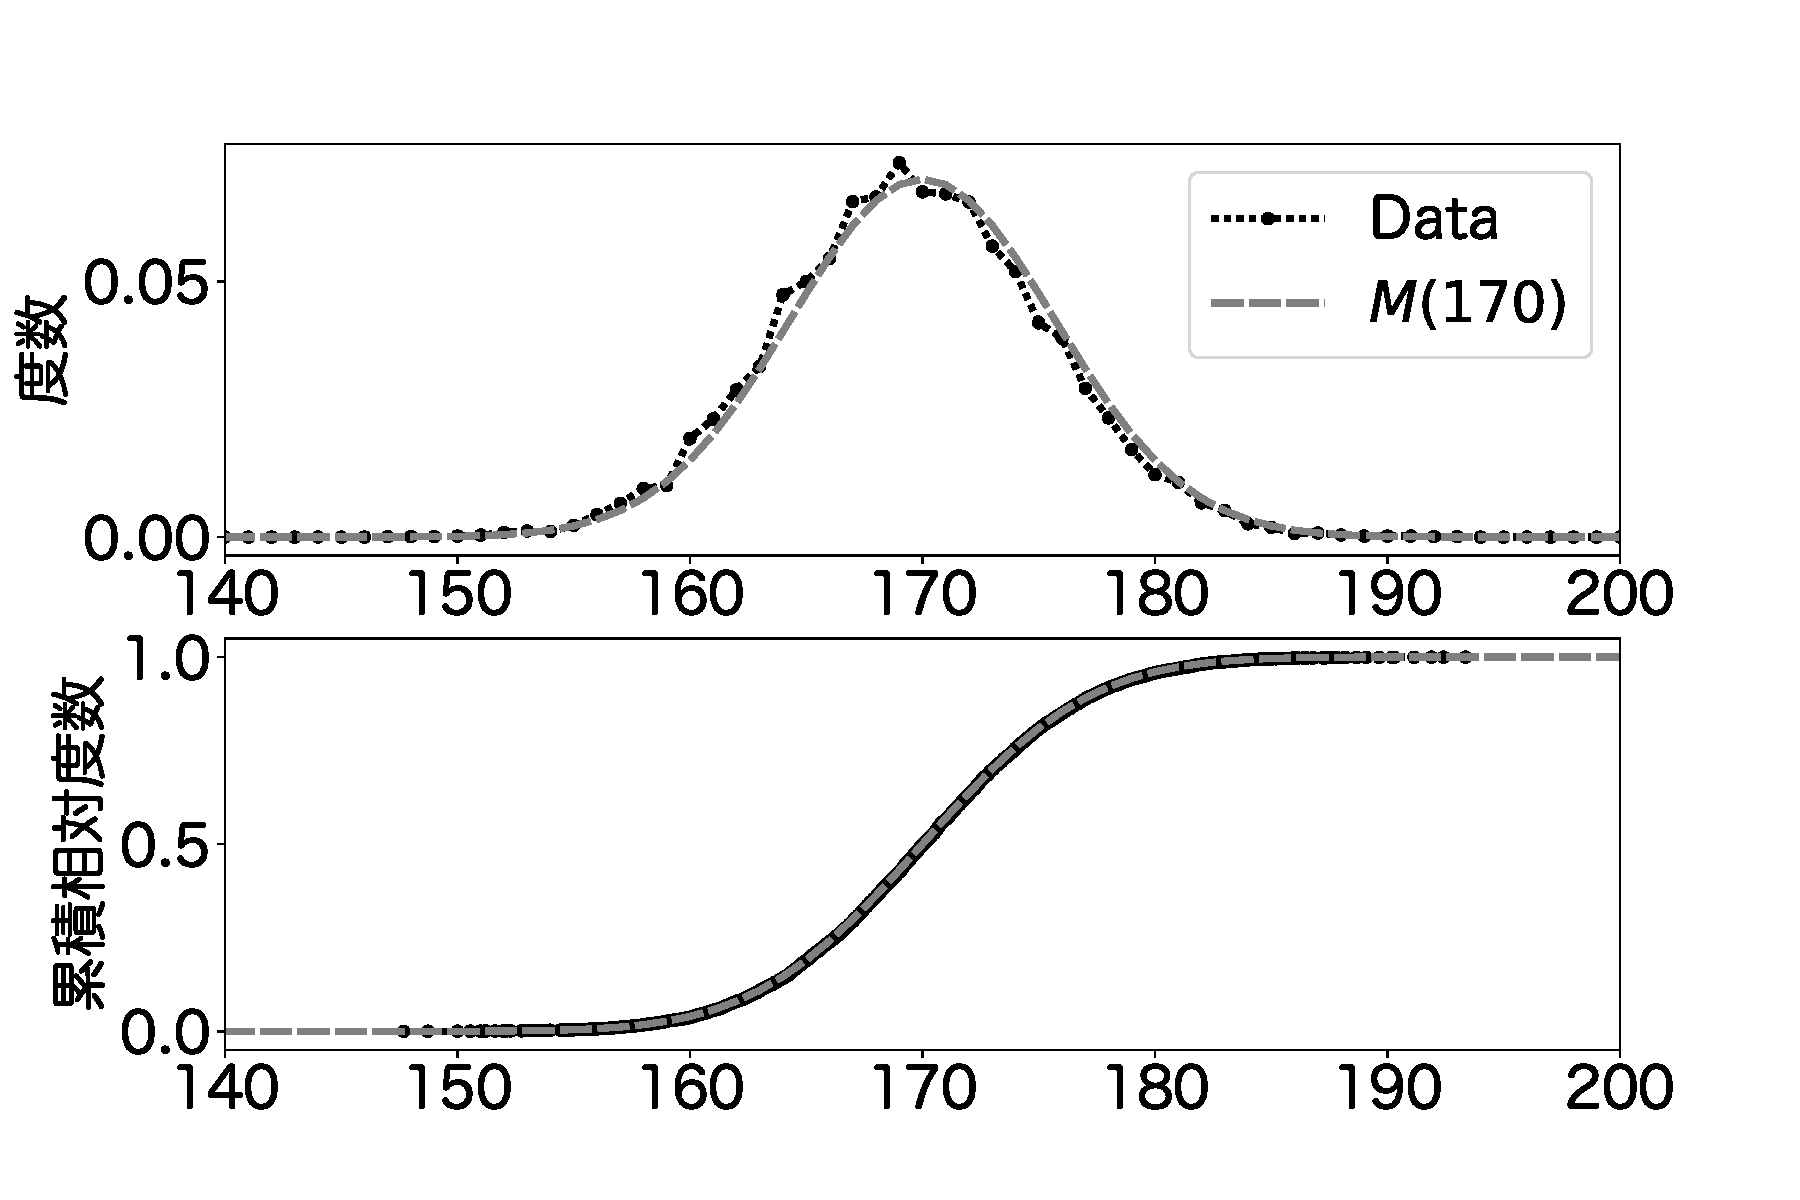
\includegraphics[width=15cm]{../markdown/section1/cm_data_simulation.pdf}
    \caption{上:正規分布を含む統計モデル$M(170)$によりサンプリングされたDataの頻度と、統計モデルの頻度。下:上と同じデータ・統計モデルの累積相対頻度}
    \label{fig:simulation_height_men}
\end{center}
\end{figure}


もう一つこの論者と私とで異なる点は、生物学データのグラフが曲線になるべきと考えているか否かである。私は、推論のために統計モデルを利用しているので、統計モデルとデータが一致しない場合でも、推測に利用できると考え、統計モデルを利用する。一方で、この論者は、統計モデルとデータが一致すべきと考えている。言い換えれば、データが統計モデルに従うことを前提にする立場と、データを推論するために統計モデルを仮定すると言う立場がある。

\if 0 
$180cm$以上の割合についてはデータと一致していますが、$160cm$以下は、データと不一致です。この統計モデルで推測できていると考えても良いのでしょうか。
無作為抽出したときに得られるデータをできます。
ここで、$\mu=169.1$の統計モデル$M(\mu=169.1)$と、$\mu=180$の統計モデル$M(180)$を
標本から無作為抽出を行い、集計すると平均$169.1cm$程度であることがわかったとします。このとき統計モデル$M(169.1)$の推測は母集団の特徴をよく捉えているだろうか?
\fi 

\begin{mybox}
\begin{quote}
\paragraph{軽いパンばかり買わされる}
ある国では、ある時期、パンを作るための道具、手順、材料が政府から配布品されパンを作ることになっていた。パンを焼くための型は、完成時に$1000g$になるように設計されており、手順を厳密に守り、計量し作ったパンは確かにおよそ$1000g$になっていた。どの季節に作っても手順を守りさえすれば、$1000g$になったのだ。
この材料、道具をパン屋が利用し、厳密に手順にそってパンを作れば、やはりパンはおよそ$1000g$になるはずである。

その国では、小麦の値段が高騰しており、パンを作らずに、小麦をそのまま売った方が儲かるという状況になっていた。そんなとき、パンが$1000g$よりも軽いと感じた数学者が、数ヶ月にわたりパンの重量を計測していった。その結果、パンの重量は平均で$950g$となっており、本来の$1000g$よりも、軽いことがわかった。このとき、パン屋は不正をしていると言えるだろうか。

手順を踏めば平均で$1000g$になるパンが平均およそ$950$になったのは、パン屋が手順通りにパンを作っていないことを疑える。手順を守って作れば$1000g$になるという経験(データ)があるから疑うことができるのである。
%もしも、季節によってパンの重さが変化するものだったとするなら、$4$月には$1000g$だったものが$6$月には、$900g$になる可能性を排除できない。
\end{quote}
\end{mybox}

\subsection{ 統計モデルの比較}
データを確認してみると、$180cm$以上の割合は、0.0642であり、統計モデル$M(171.1)$の推測値$P(x>180)=0.059$と数値が近いことがわかります。
また$160cm$以下の割合は、$0.023$程度であり、統計モデルの推測値$P(x<160)=0.025$であり、やはり数値が近いことがわかります。
このように数学的フィクションである統計モデルを使うことで、現実に関する推測が可能になったことがわかります。


ここまでは、$M(171.1)$を用いて、母集団の推測を行いました。統計モデル$M(170)$の代わりに$M(168)$により推測を行うとどうなるでしょうか。$180cm$以上の人を推測すると$M(168)$では$P(x>180)=0.03$であり、統計モデル$M(171.1)$の推測$P(x>180)=0.059$よりもさらに実際の計測値$0.0642$と乖離していることが分かります。
これは、$M(168)$では、ピークが平均値の$168$に移動するので、$180cm$を超える割合がさらに低くなるので当然です。

一方で、$160$以下の人では、$M(168)$では、$P(x<160)=0.08$程であり、$M(171.1)$の推測値$P(x<160)=0.025$よりも、実際の数値$0.023$から離れていることがわかります。
これも、$M(168)$では、ピークが$170$よりも小さな値になるので、$160cm$より小さい人の割合が大きくなるので当然です。

\begin{table}[hbtp]
    \caption{統計モデルとデータの比較}
    \label{table:data_type}
    \centering
    \begin{tabular}{lcc}
    %\hline
    統計モデル  & $P(x<160)$  & $P(x>180)$   \\
    \hline \hline
    データ &  0.023 &  0.0642\\
      %\hline \hline
    M(171.1) & 0.025 & 0.059  \\
    M(168) &  0.08 & 0.03 \\
      \hline
    \end{tabular}
  \end{table}

このように、統計モデルの母数に応じて、現実の予測精度が変化することがわかります。
この統計モデルの予測の良さが分かったのは、無作為抽出を繰り返して、サンプルサイズを大きくしたときのデータの分布を得ていることによって、
そのデータとモデルとを比較をすることで、$M(171.1)$が$M(168)$より良い統計モデルであることを判別できました。

では、データが十分でない場合においても、推測とデータの一致を基準にして、より良い統計モデルを選ぶことはできるのでしょうか?
\subsection{統計モデル選択}
\subsubsection{推測値とデータの比較}
母集団のことをほとんど知らない場合は、どちらの統計モデルが良いモデルであるか調べることは可能でしょうか?
ここでは、17歳の日本人男性の身長を対象とします。
母集団に関して次のことを知っていることにします。
\begin{itemize}
    \item 平均がおよそ$170cm$
    \item $160cm$の人や$180cm$の人と出会う確率は同じくらい($170cm$を中心に対象に分布している)
    \item 分散は5.7
\end{itemize}

サンプルサイズ10の標本が二つ得られたとします(実際には、コンピュータを使って正規分布からサンプリングした。本書では母集団から無作為抽出したと考える)。一つめの標本は、次の通りです。

\begin{lstlisting}
sample1 = [162.56944902, 178.42128764, 171.15286336, 172.2581195 , 160.21499345, 175.35072013, 173.17952774, 173.73301156, 179.52758126, 178.35924221]
\end{lstlisting}


もう一つの標本は、次のようなサンプルが得られました。
\begin{lstlisting}
sample2 = [164.04222157, 162.19052559, 172.03420244, 168.03580415, 176.73750537, 166.41177205, 165.27050656, 168.02537023, 176.18720054, 171.78005419]
\end{lstlisting}


\begin{table}[hbtp]
    \caption{統計モデルと小さいサンプルサイズの標本}
    \label{table:smalle_sample_size}
    \centering
    \begin{tabular}{lccc}
    %\hline
    統計モデル  & $P(x<160)$  & $P(x>180)$  & $\bar{X}$ \\
    \hline \hline
    標本1 &  0 &  0 & 172.8 \\
    標本2 &  0 &  0 & 169 \\
      %\hline \hline
    M(171.1) & 0.025 & 0.059  & 171.1 \\
    M(168) &  0.08 & 0.03 & 168\\
      \hline
    \end{tabular}
  \end{table}
一つめの標本では$180cm$以上の人は、$0$人で、$160cm$以下の人も$0$人で、どちらの統計モデルでも推測と一致しているかを考えることができません[表\ref{table:smalle_sample_size}]。
標本平均$\bar{X}=172.8$であり、$M(170)$の母数$170$が$M(168)$の母数平均$168cm$より近いことがわかります。

二つめの標本では$180cm$以上の人は、$0$人で、$160cm$以下の人も$0$人で、どちらの統計モデルでも推測と一致しているかを考えることができません。
標本平均$\bar{X}=169.0$であり、$M(170)$の母数$170$と$M(168)$の母数平均$168cm$の差が$1cm$でどちらも同じ程度です。

サンプルサイズが小さいときには、統計モデルの予測とデータを比較できないことがあるので、予測精度の良いモデルを推定することができません。

% また、標本の平均値と統計モデルの平均値でも標本が
% 仮説検定の枠組みでは、絶対にだめな統計モデルを明らかにします。

%\subsubsection{標本内の偏った値に注目}



\subsection{統計モデルの性質を使った方法}
ここまでは、統計モデルの予測がデータと一致するかを扱った。ここでは、データを統計モデル上に持って行ったとき、そのデータ以上大きな値を取る確率を計算し、その確率が低ければ、だめなモデルと判定する方法を議論する。

今回考えている統計モデル$M(\mu)$では、次の統計量$Z$が標準正規分布$N(0,1)$に従うことが、正規分布の再生性によってわかっている。
\if 0
 川久保統計学P.166
 \fi
$$
Z(\bar{X},\mu)=\frac{\sqrt{n}(\bar{X}-\mu)}{\sigma} \sim N(0,1)
$$
ここで$\bar{X}$は、統計モデル$M(\mu)$からサンプリングしたときの標本平均値(データの平均値ではない)、$\mu,\sigma$は統計モデルで設定した母数平均、母数分散。
$Z(\bar{X},\mu)$が$N(0,1)$に従うということは、$Z(\bar{X},\mu)$が$N(0,1)$において、どれくらいの頻度で出てくるのかが計算できます。

%![Z値の頻度]()
\begin{figure}
\begin{center}
    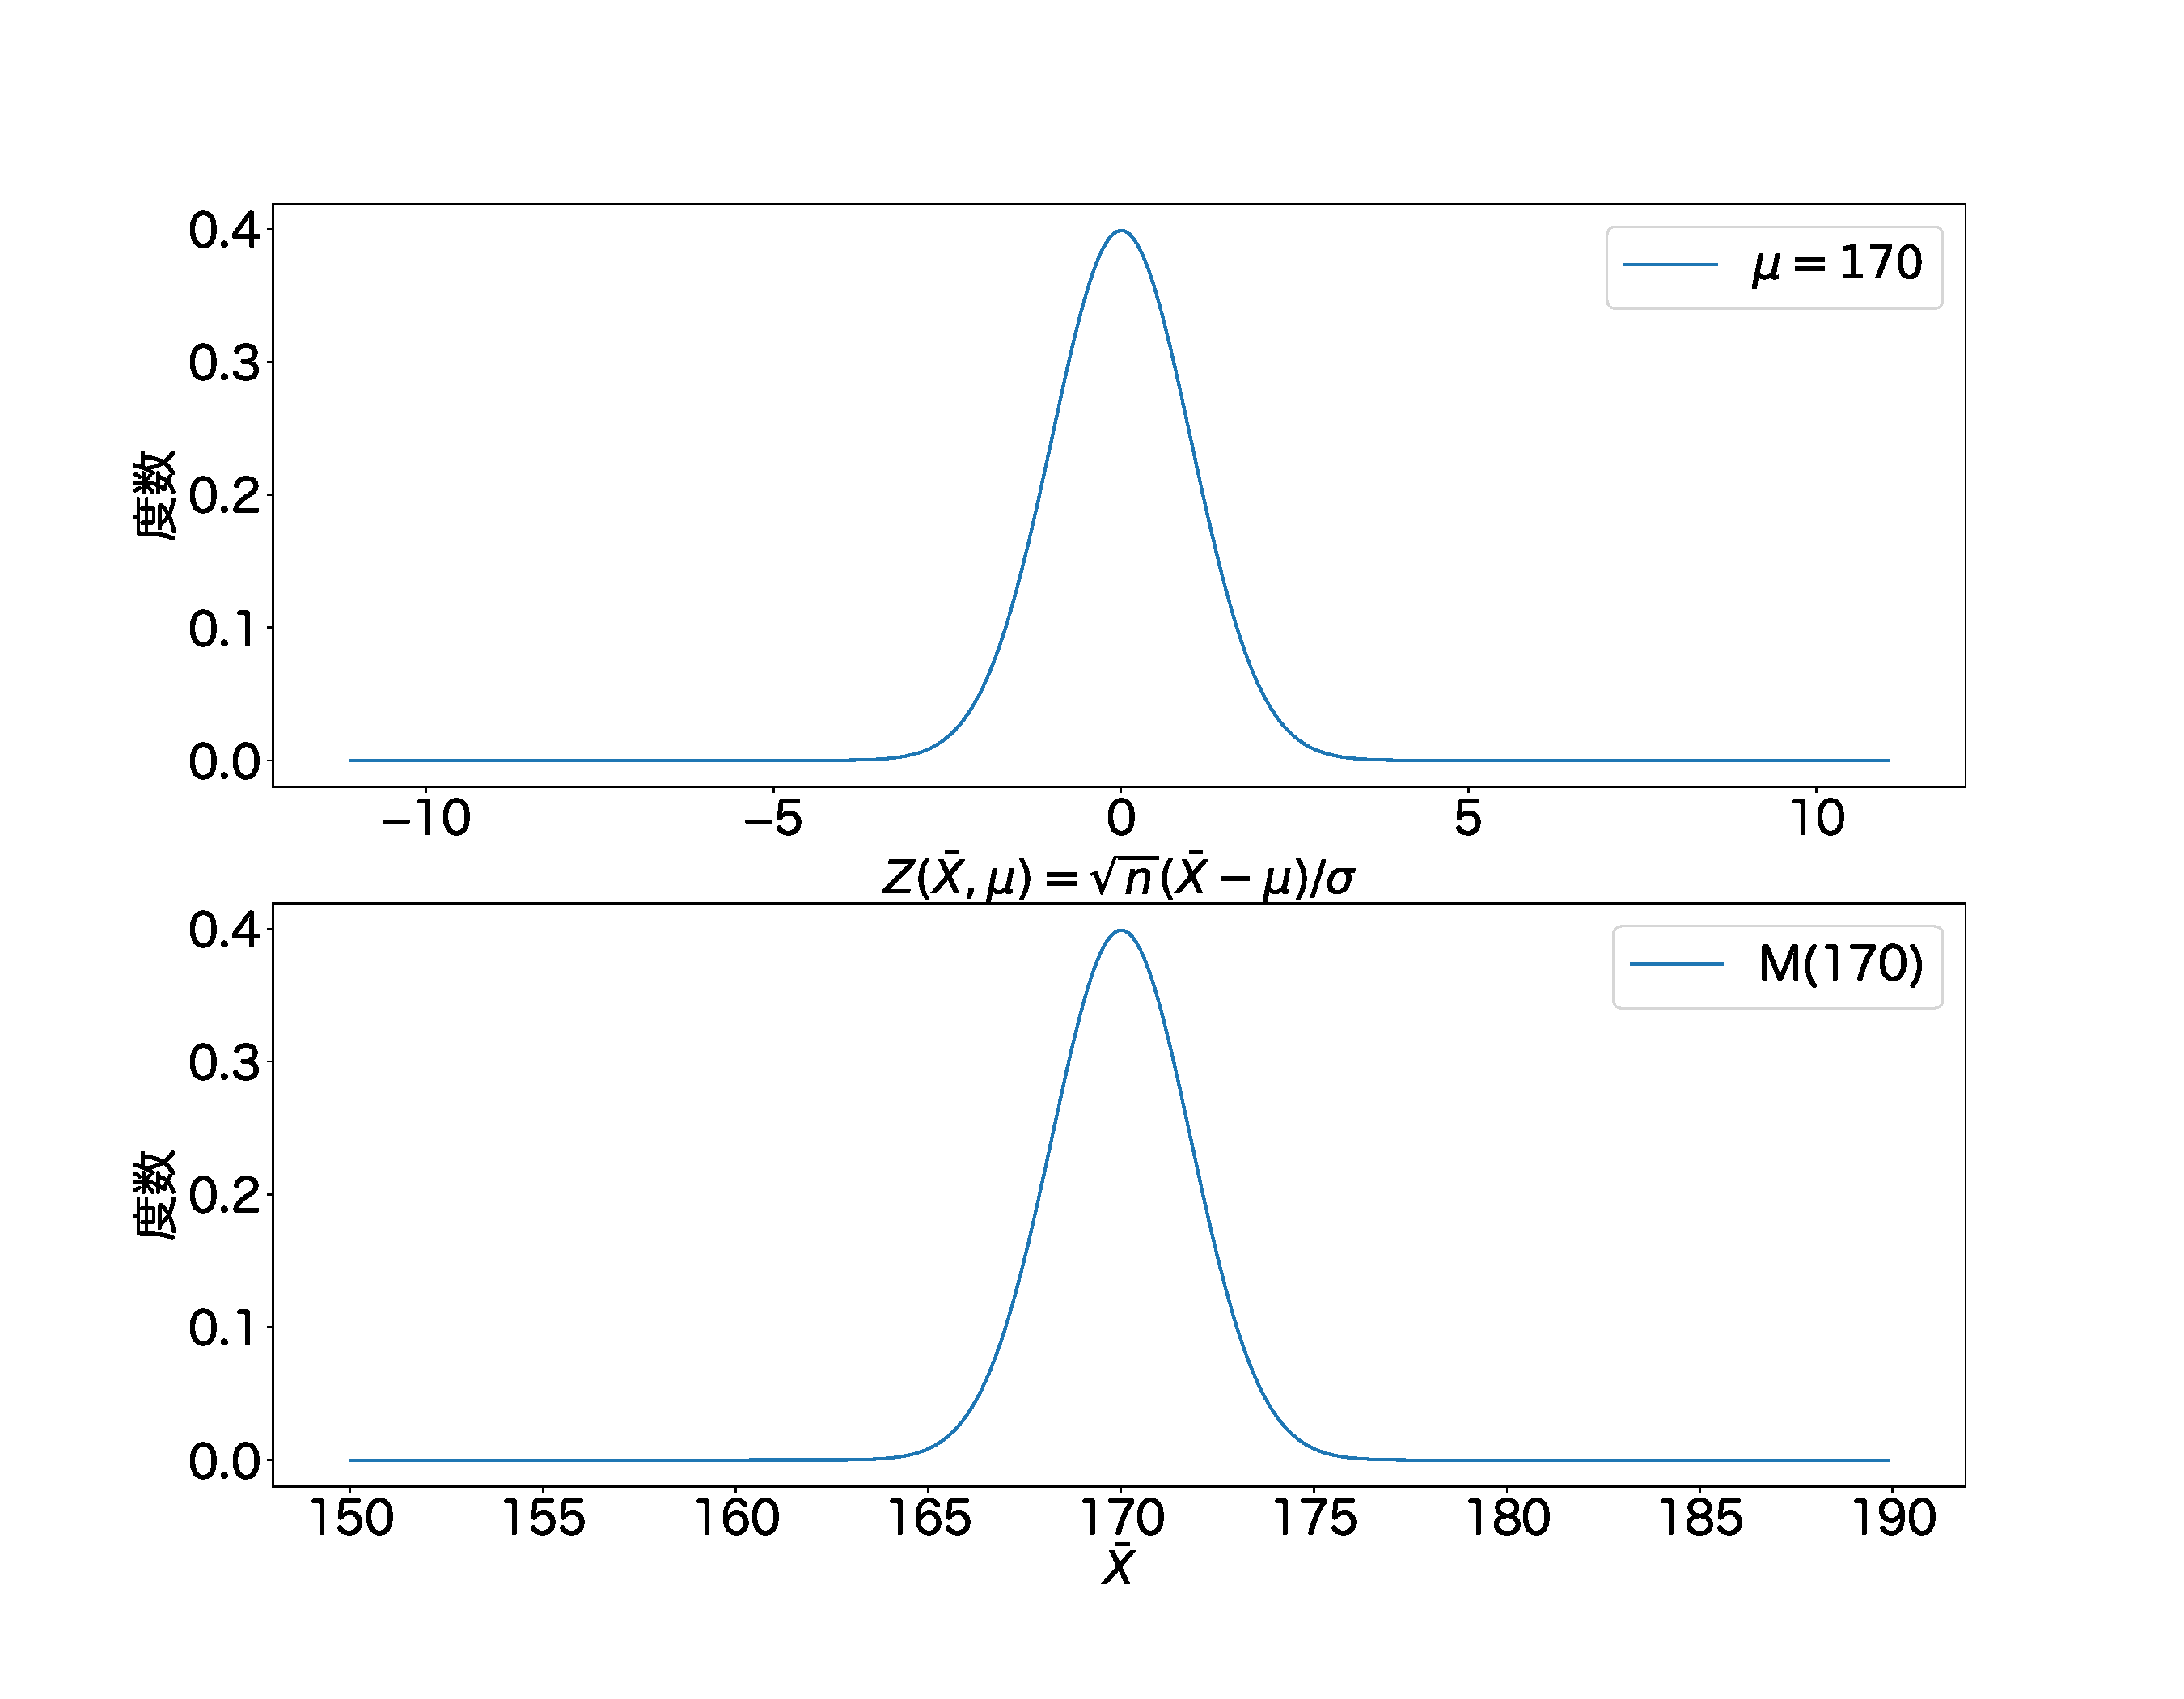
\includegraphics[width=15cm]{../markdown/section1/normal_Z_frequency.pdf}
  \end{center}
\end{figure}

$Z$の出現頻度を$Z$または$\bar{X}$の値に応じて書いたものが図です。
$Z(\bar{X},\mu)$が出現しやすい範囲は、
$$
-z_{0.025}<Z(\bar{X},\mu)<z_{0.025}
$$
の範囲で、この間で$95\%$の確率でサンプリングされた標本の平均$\bar{x}$が観測されます。
$95\%$を採用したのは、統計モデルを使った判断で、よく出てくる確率として分野を問わず、$95\%$が使われているからです。
%この値には身長に関する経験を使わずに決定しています。

また、統計モデルからサンプリングしたときの、標本平均がどのあたりにあるのかが計算できます。式を変形してみます。
\begin{eqnarray*}
    & -z_{0.025} < Z(\bar{X},\mu)<z_{0.025} \\
\rightarrow & -z_{0.025} < \frac{\sqrt{n}(\bar{X}-\mu)}{\sigma}  <z_{0.025} \\
\rightarrow & \mu - z_{0.025} \frac{\sigma}{\sqrt{n}} < \bar{X} < \mu + z_{0.025} \frac{\sigma}{\sqrt{n}}
\end{eqnarray*}

この統計モデルによって計算できたサンプルの平均値$\bar{x}$が$95\%$の確率で見つかる範囲のことを信頼区間と言います。
このことから、統計モデル$M(\mu)$でサンプリングしたときに、$95\%$の確率で、この範囲に平均値$\bar{X}$がえられます。

\subsubsection{サンプルサイズによる影響}
式を見てわかるように、サンプルサイズ$n$が大きくなれば、$\bar{x}$が入る範囲は狭くなります。

信頼区間がサンプルサイズに依存することを確認しておこう。
図は、信頼区間を各Nに応じて変化する様子を図示している。$N=1$では、$\bar{x}$が$154\sim185$あたりであれば、$M(170)$は棄却できない。$N=4$であれば、$\bar{x}$が$162\sim177$であれば、$M(170)$は棄却できない。$N=10$であれば、$\bar{x}$が$165\sim174$であれば、$M(170)$は棄却できない。
このようにサンプルサイズが増加することで、信頼区間が狭まり、棄却できるモデルの母数の範囲が狭まることがわかる。
\begin{figure}

\begin{center}
    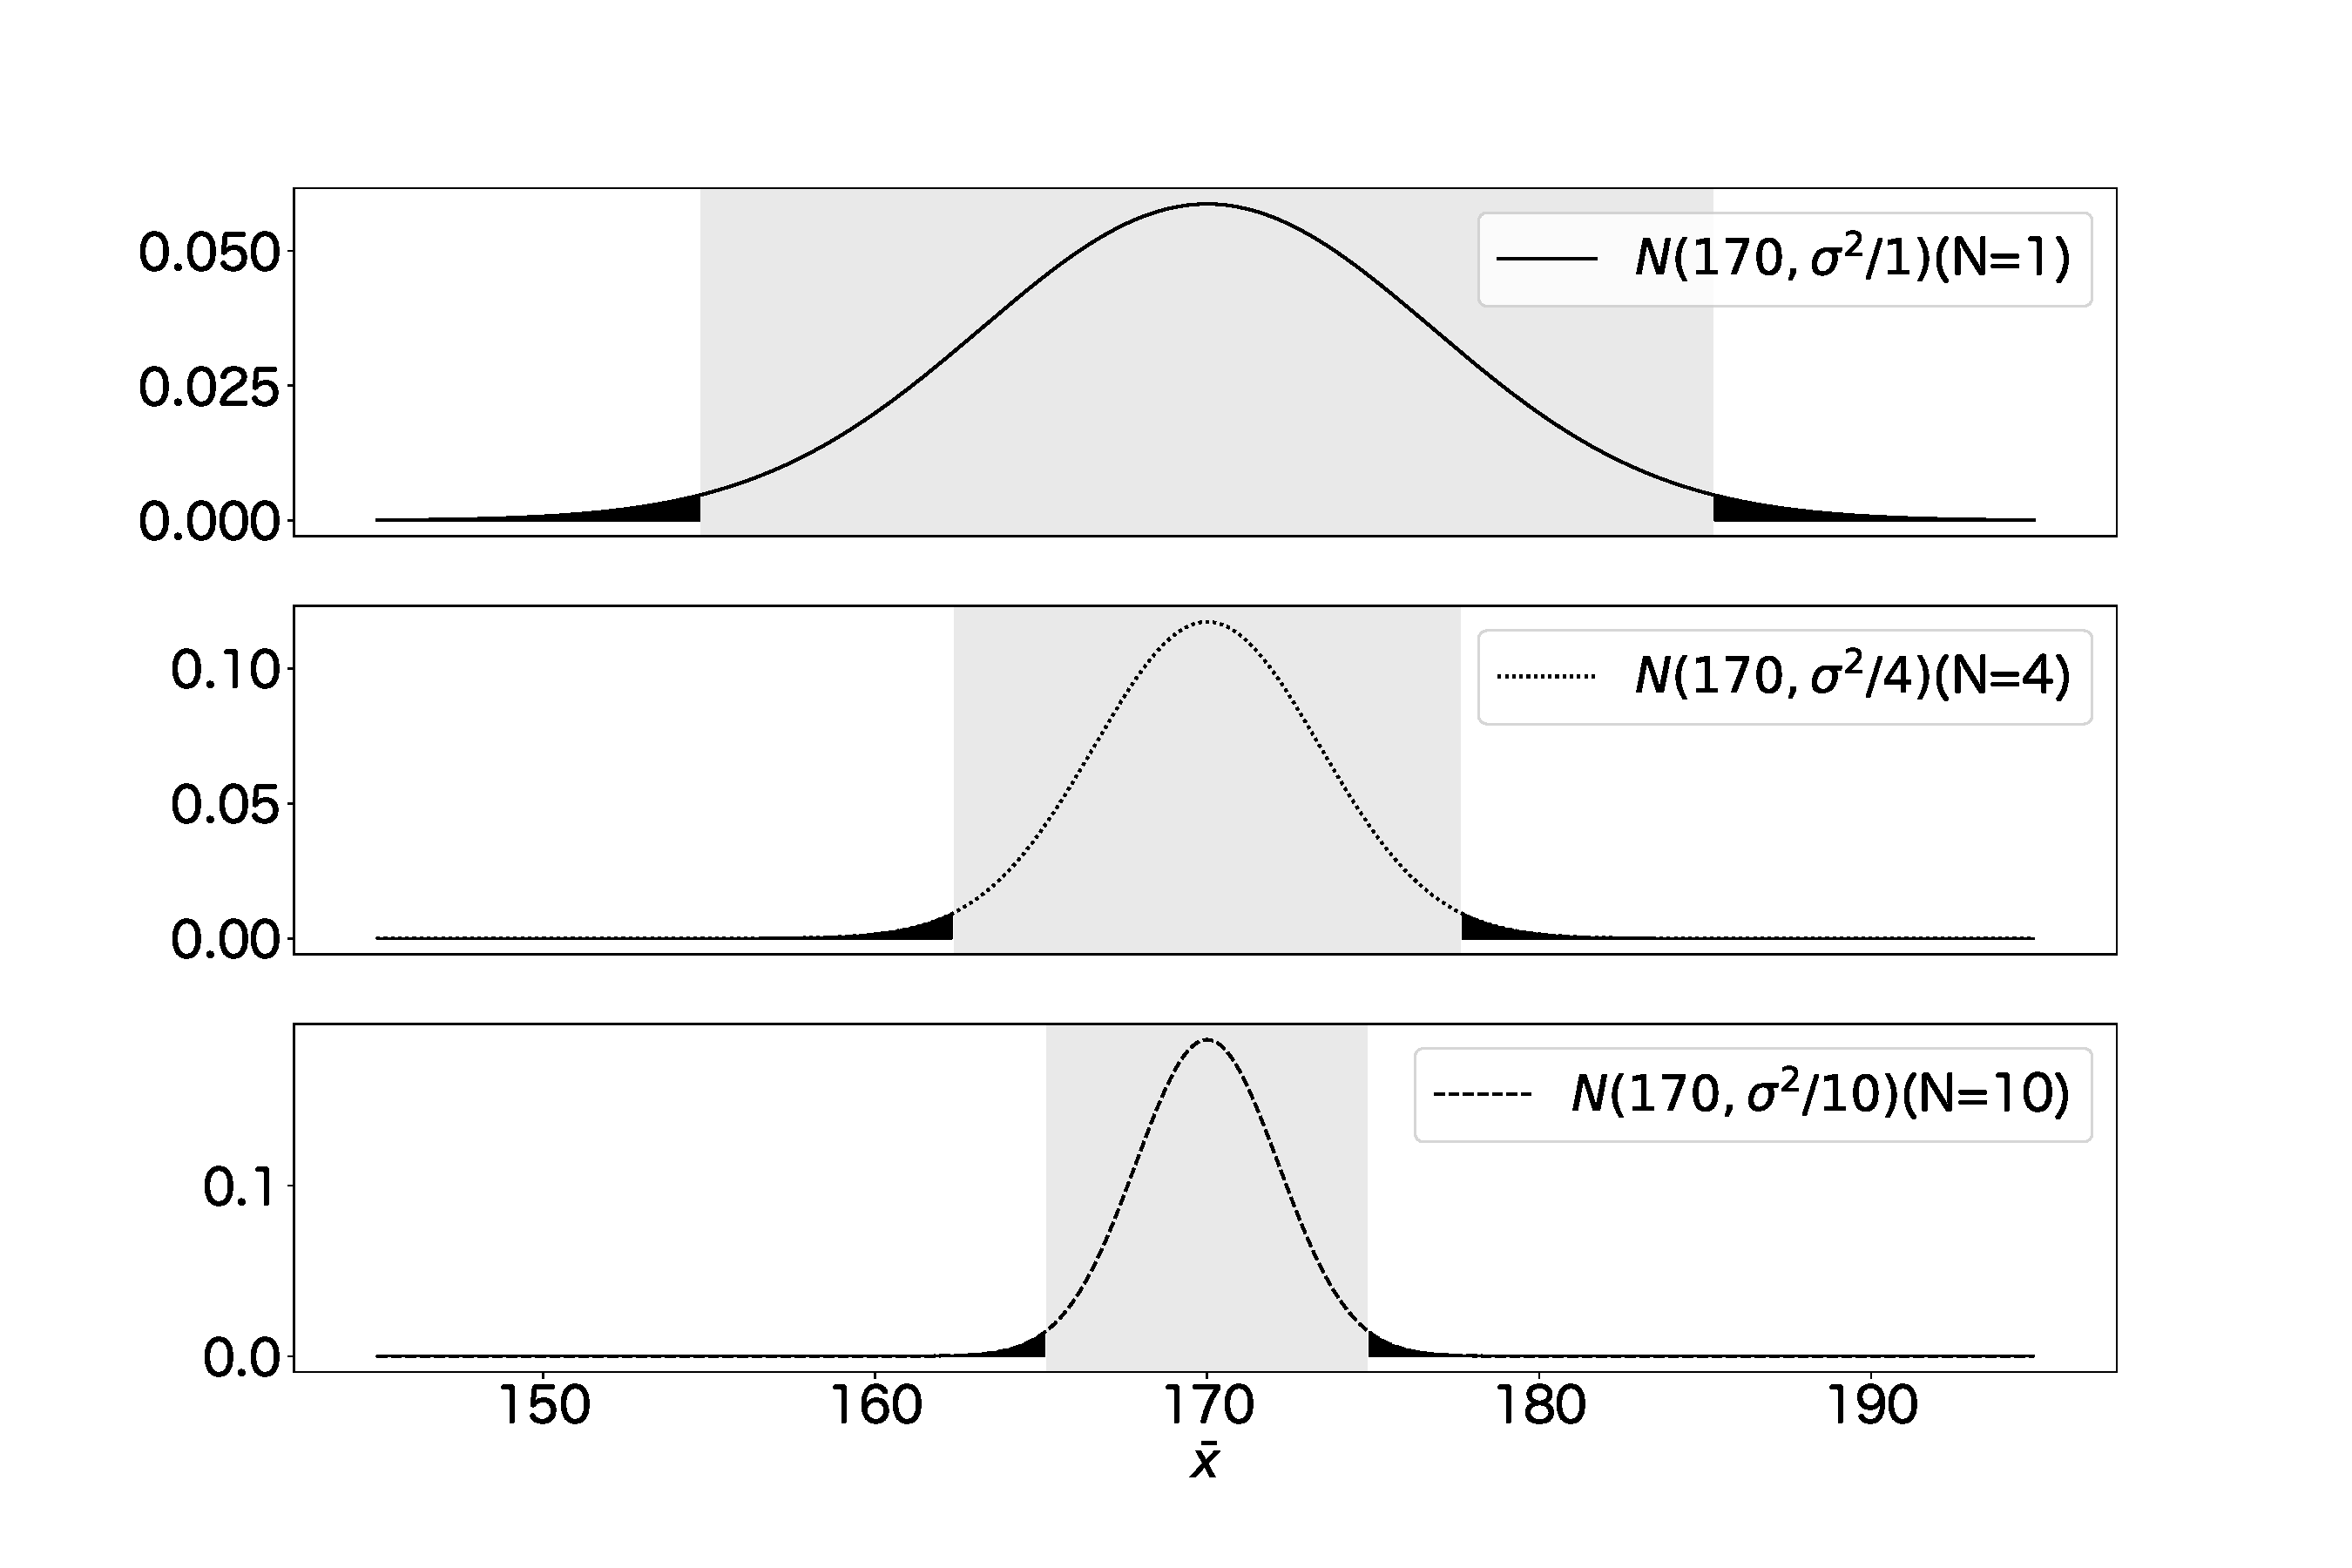
\includegraphics[width=15cm]{../markdown/section1/confidence_interval.pdf}
    %\caption{信頼区間}
  \end{center}
\end{figure}


実際に、$M(\mu=170)$を使って、$サンプルサイズを10$とし、標本を$100$個作ってみると、その分布は、図(B)のようになった。それぞれの標本に対してその信頼区間を描いたものが図(A)である。図Aの170cmのところにある縦の線は、統計モデル$M(\mu=170)$の母数平均である。
この170cmを跨いでいる信頼区間の個数はこの図では$96$個ある。コンピュータシミュレーションをするたびに毎回跨いでいる信頼区間の個数は変化するがおよそ95個である。このことは、信頼区間の定義から明らかである。


\begin{figure}
\begin{center}
    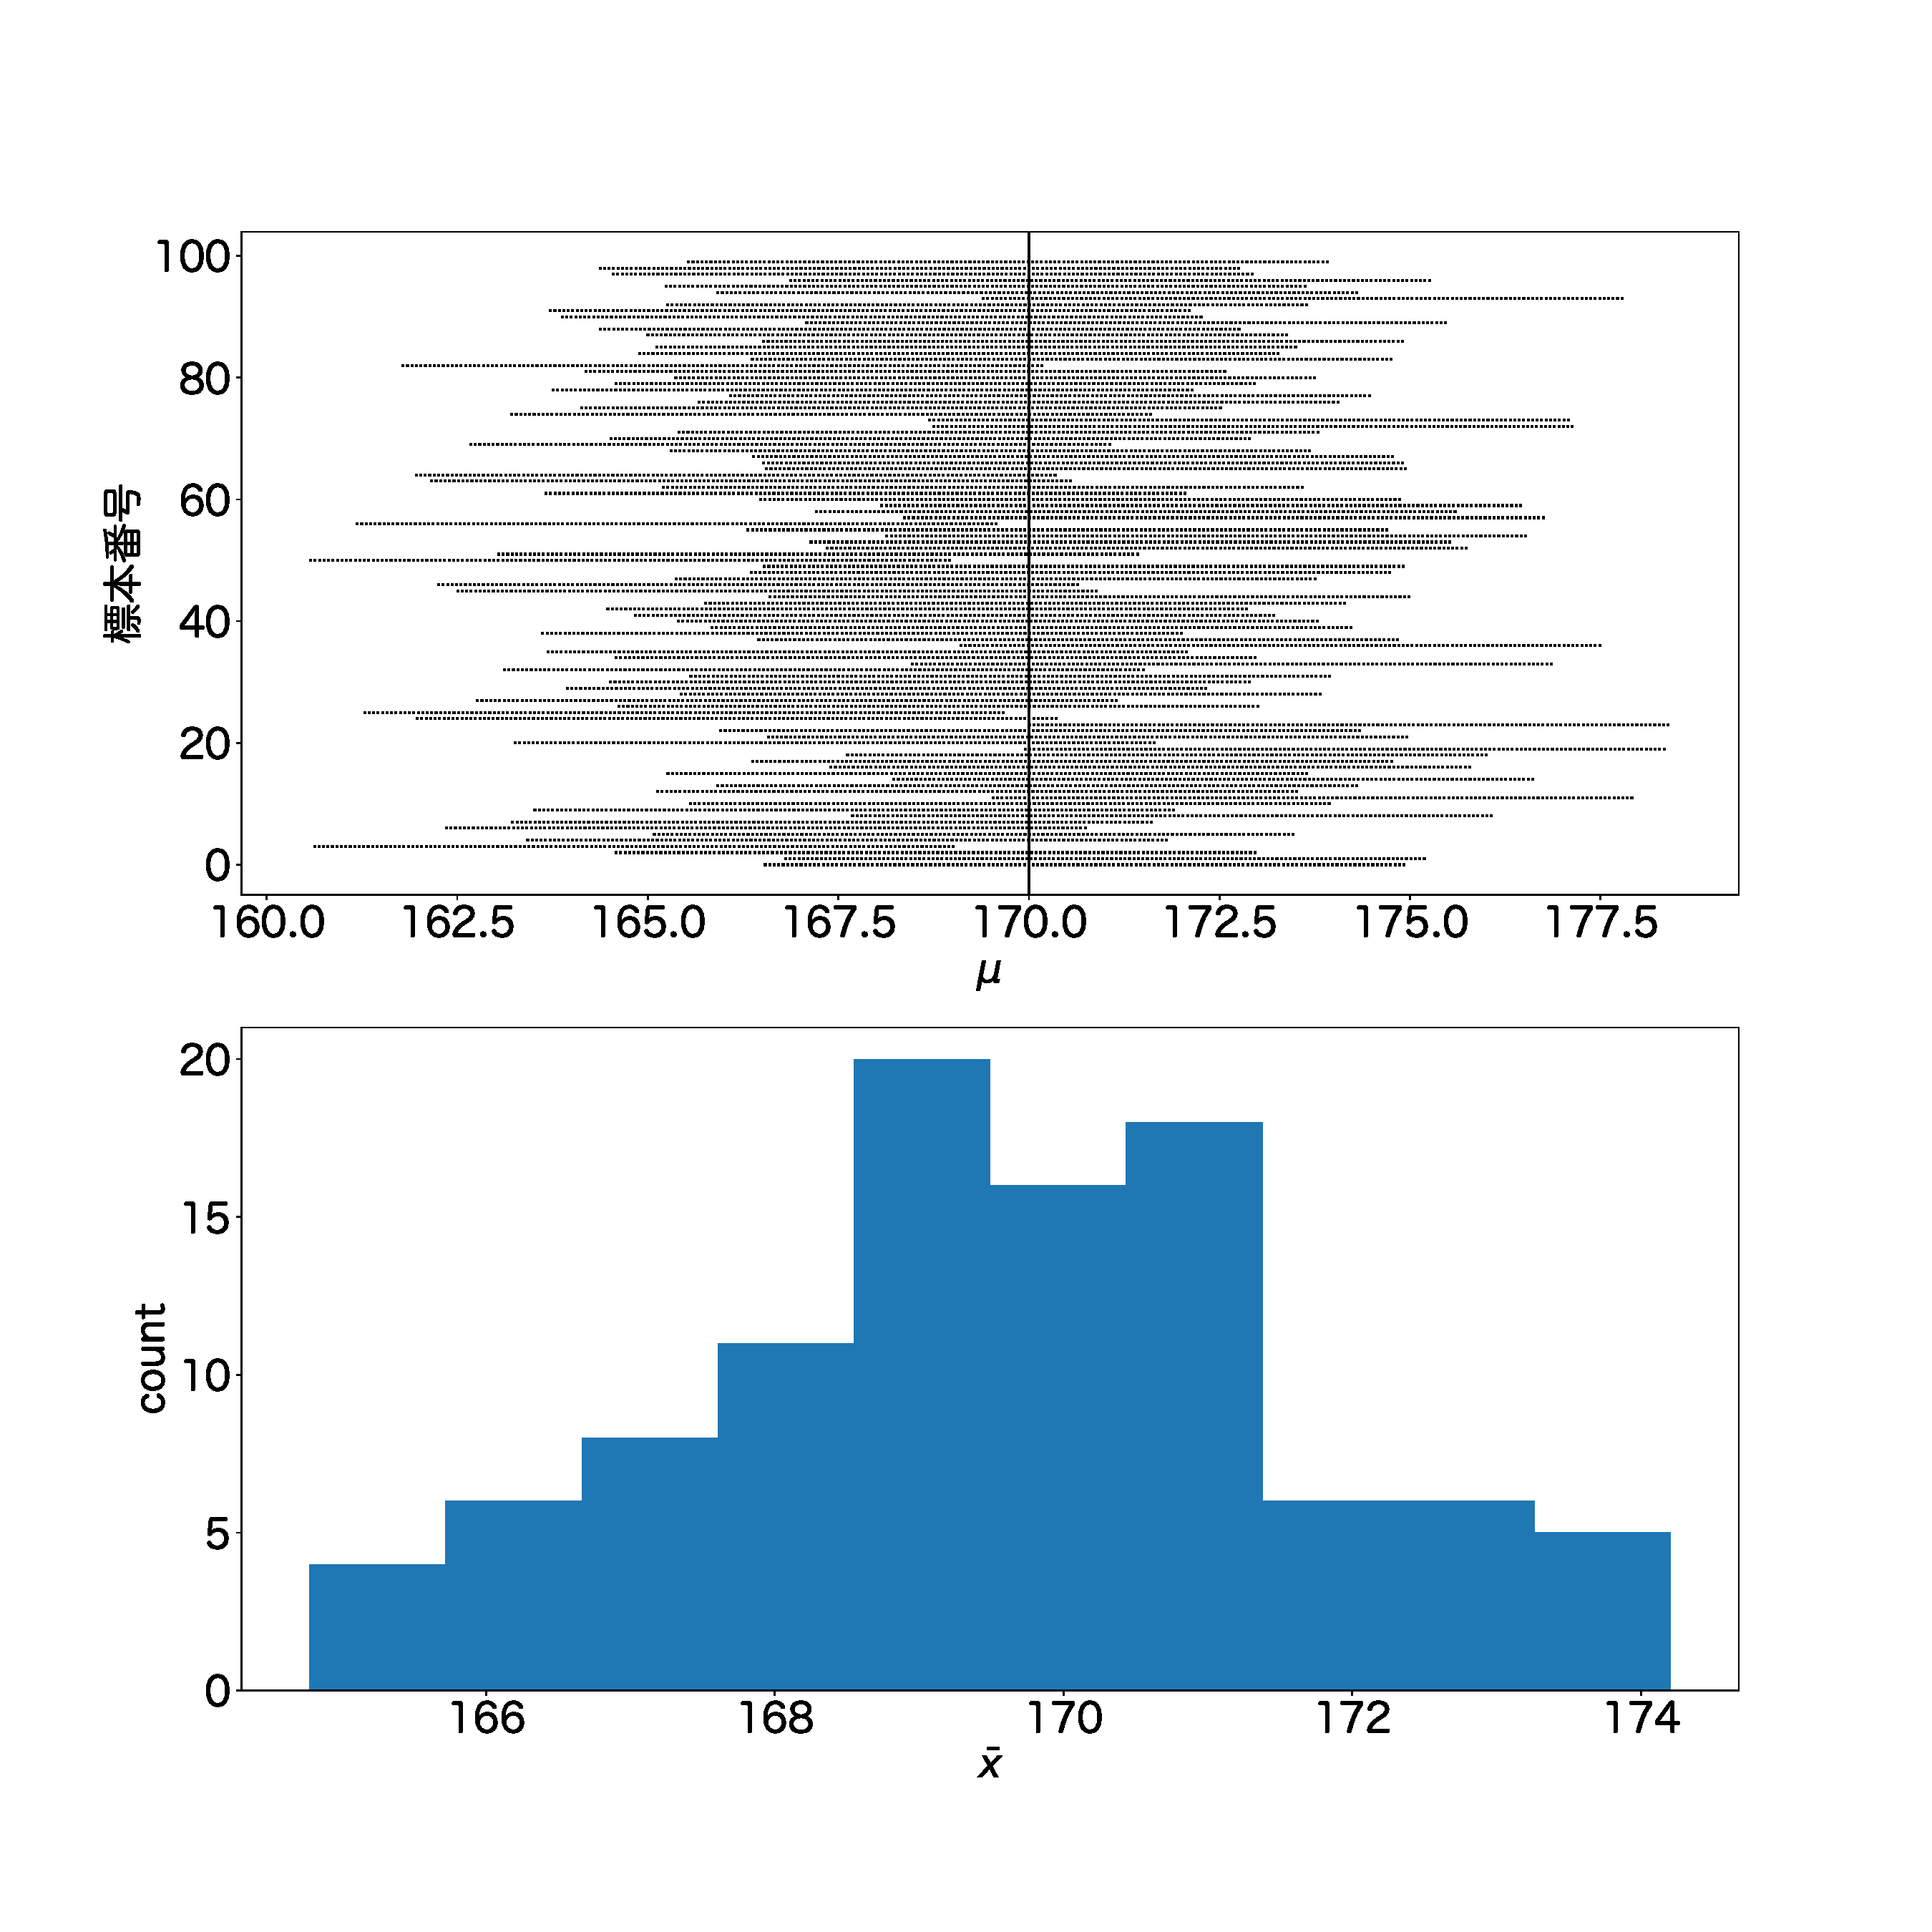
\includegraphics[width=15cm]{../markdown/section1/confidence_interval_model_count.pdf}
  \end{center}
\end{figure}


\begin{mybox}
    \begin{quotation}
        \paragraph{信頼区間は、データをたくさん取ったときに(サンプルサイズを大きくしたのではなく、サンプルサイズが同じ標本をたくさん集めたときに)、その範囲に真値が$95\%$の確率で含まれるの区間のこと}
        信頼区間は、データをたくさん取ったときに、その範囲に真値が入る$95\%$の確率で含まれるの区間のこと\footnote{\url{https://www.slideshare.net/simizu706/ss-123679555}}。このように解説されることがあります。

        一般に、母集団を統計モデルにより、よく推測できる場合では、確かに$95\%$くらいの確率で無作為抽出した標本の標本平均が含まれます。一方で、統計モデルが現象をよく推測している場合でも、母数を出鱈目に変化させた統計モデルを作るとします。新たな統計モデルでは、無作為抽出した標本の標本平均がその信頼区間に含まれる頻度は低くなります。
        また、統計モデルが現象をよく推測できない場合では、$95\%$信頼区間にモデルの母数が含まれる確率は低くなると思われます。

        以上のことから、私は、信頼区間は、データをたくさん取ったときに、その範囲に真値が$95\%$の確率で含まれるの区間のことという解釈はやめておいた方がいいと思っています。
    \end{quotation}
\end{mybox}


\begin{framed}
まとめ、
\begin{itemize}
    \item 統計モデル$M(\mu)$によってサンプリングし、標本を得たとき、その平均値のよくある値の範囲(信頼区間)が計算できた
\end{itemize}
\end{framed}

\subsubsection{モデルを基準にしたデータと統計モデルの比較}
ここからは、母集団から無作為抽出したデータについて考えます。
無作為抽出によって得られた標本のサンプル$x_1,x_2,\cdots,x_n$について、その平均値を$\bar{x}$とします。
$M(171)$において、$\bar{x}=172$の場合($\phi(z)$を標準正規分布とする)、$\phi(z>\frac{\sqrt{n}(\bar{x}-\mu)}{\sigma}) = 0.289$であり、$\bar{x}=169$の場合、$\phi(z>\frac{\sqrt{n}(\bar{x}-\mu)}{\sigma}) = 0.133$です。このことから、統計モデル$M(\mu)$において、これらの観測値はそこまで稀ではありません。$M(168)$でも同様に計算できます。

\begin{lstlisting}
    xbar = 172
    mu=171
    sigma = 5.7
    N=10
    c = np.sqrt(N)*(xbar-mu)/sigma
    1-norm.cdf(c,0,1)
\end{lstlisting}
    


\subsubsection{統計モデルを基準にしたデータと統計モデルの比較}
統計量$Z(\bar{X},\mu)$がよく入る区間の式を変形し、データを得たときに、そのデータを基準にした$\mu$の範囲に変形してみます。
\begin{eqnarray*}
 & -z_{0.025} < Z(\bar{X},\mu)<z_{0.025} \\
\rightarrow & -z_{0.025} < \frac{\sqrt{n}(\bar{X}-\mu)}{\sigma}  <z_{0.025} \\
\rightarrow & \bar{x}- z_{0.025}\frac{\sigma}{\sqrt{n}} < \mu < \bar{x} + z_{0.025}\frac{\sigma}{\sqrt{n}}
\end{eqnarray*}
標本$1$標本$2$について、これを計算してみる。平均値は、それぞれ172.4, 169.0です。
標本$1$では、$168.9 < \mu < 176.0$、標本$2$では、$165.5 < \mu <172.6$です。
この範囲にある$\mu$をもつ統計モデルであれば、データをよくある範囲に入れることができます。
例えば、$M(168)$でも標本$1,2$の平均値はよくある範囲に収まります。

まとめ、
\begin{framed}
    \begin{itemize}
        \item 統計モデル$M(\mu)$のサンプルの平均が$95\%$の確率で入る範囲$\mu - z_{0.025} \frac{\sigma}{\sqrt{n}} < \bar{X} < \mu + z_{0.025} \frac{\sigma}{\sqrt{n}}$。現実の母集団が統計モデルによってよく推測できるなら、この範囲に平均値が入る確率は$95\%$に近くなることもある。逆に、統計モデルが現実をよく捉えることができなければ、母集団から無作為抽出した標本の平均値はこの範囲に入ることは少なくなる。
        \item データがよくある範囲に入る統計モデル$M(\mu)$の$\mu$の範囲$\bar{x}- z_{0.025}\frac{\sigma}{\sqrt{n}} < \mu < \bar{x} + z_{0.025}\frac{\sigma}{\sqrt{n}}$
        \item  統計モデル$M(\mu)$ではサンプルサイズを大きくすると、平均値が入る範囲が狭くなる。
    \end{itemize}
\end{framed}

\subsubsection{$Z(\bar{x},\mu)$以上の値が得られる確率}
$Z(\bar{x},\mu)\sim N(0,1)$により、$Z$以上の値が得られる確率も計算できます。つまり、
\begin{equation*}
    p = \varPhi(Z(\bar{x},\mu)>x)
\end{equation*}
です。$\bar{x}=172.4,\mu=168,\sigma^2=6.8,n=10$であれば、$Z(\bar{x},\mu)=2.04$であり、
$p=0.04$です。

\begin{lstlisting}
xbar = 172.4
mu = 168
sigma2 = 6.8**2
n=10
Z = np.sqrt(n)*(xbar-mu)/np.sqrt(sigma2)
print(Z)
p=1-norm.cdf(Z,0,1)
print(p*2)
\end{lstlisting}


\section{統計的仮説検定}
ここまで、推測ができるまたは、データが統計モデルにおいてよくある値なのかを利用し、統計モデルの良さを評価し、良いモデルを選択しようとした。
統計的仮説検定では、絶対にダメな統計モデルを調べる方法である。
\begin{defi}
    データと統計モデルを比較して、絶対にだめと判断されたとき、統計モデルを棄却すると宣言する。絶対にダメと判断されないときは、統計モデルを採択(棄却の対義語)するとは宣言しない。統計モデルが棄却されるのは、統計モデルの仮定によって変化する。本書の範囲内であれば、統計モデルの母数、分布関数、独立同一の分布関数からサンプリングされたことによる。特に、統計モデルの母数の変化によって決まる棄却される母数の範囲を棄却域といい、棄却されない母数の範囲を信頼区間という。サンプルから得られる統計量以上の値が得られる確率を$p$値と呼ぶ。棄却される$p$値の閾値を有意水準$\alpha$と言い、一般に$\alpha=0.05$が使われる。統計モデルの分布関数が変化すれば、その統計モデルにおける信頼区間・棄却域・$p$値の計算方法も変わる。
\end{defi}

\if 0 
これらの事象は、統計モデルの上で観測される、数学的な事実です。
数学を扱っている以上はこの事実は決して崩れることはありえません。
一方で、我々が扱う現象ではどうなるでしょうか。現象が数学な分布関数から生成されていることは決してありえません。
誰かがサイコロを振って、人々の身長を決めているのなら話は別ですが、
人の身長が、ランダムに正規分布によって決定されることはありませんね。

$M(168)$モデルの平均値は$168cm$、データでは$171cm$程度なので、$3cm$小さい。また、
$180cm$以上の人の割合を使ってモデルとデータの乖離を調べることができました。
$180cm$の人がたまたまいなかった場合は、$M(169.1),M(168)$のどちらも推測できているとは言い難いことになります。このことから、特定の値を使って乖離を判定することは難しいと考えられます。


$\phi(z>Z(\mu))を$p値として、絶対に選択してはいけない統計モデル$M(\mu)$の母数$\mu$を調べます。具体的には、指標$p$が$0.05$より小さい統計モデルを選択しないようにします。その母数の範囲は$162.14 >\mu, \mu > 174.31$です。この母数の統計モデルは$p=0.05$の基準で使わないことを統計モデルを棄却すると言います。逆に、$p>0.05$となるモデルは、積極的に正しいとは考えません。明らかに間違いではないけども正しくもないという判断をします。


$p$値を使う方法がとられます。p値とは統計モデルとデータの乖離度合いを示す指標です。p値は$0~1$の値をとり、$0$に近いと統計モデルとデータが乖離していると判断します。
\fi 

これまでは、統計モデル$M(\mu)$における信頼区間・棄却域の計算を行ってきました。今回は、$p$値を計算します。
無作為抽出により得られたデータ$\bar{x}$がこれ以上偏る確率は、
$\phi(z>\frac{\sqrt{n}(\bar{x}-\mu)}{\sigma})$
により計算できます。

図1は、$\mu$を変数にし、各$\mu$に対して、$\phi(z>Z(\mu))$を示します。標本平均$168.7cm$をピークに左右対象に$\phi(z>Z(\mu))$が減少していることが分かります。つまり、$M(168.7)$が最も乖離の度合いが小さい統計モデルです。
\begin{figure}
\begin{center}
   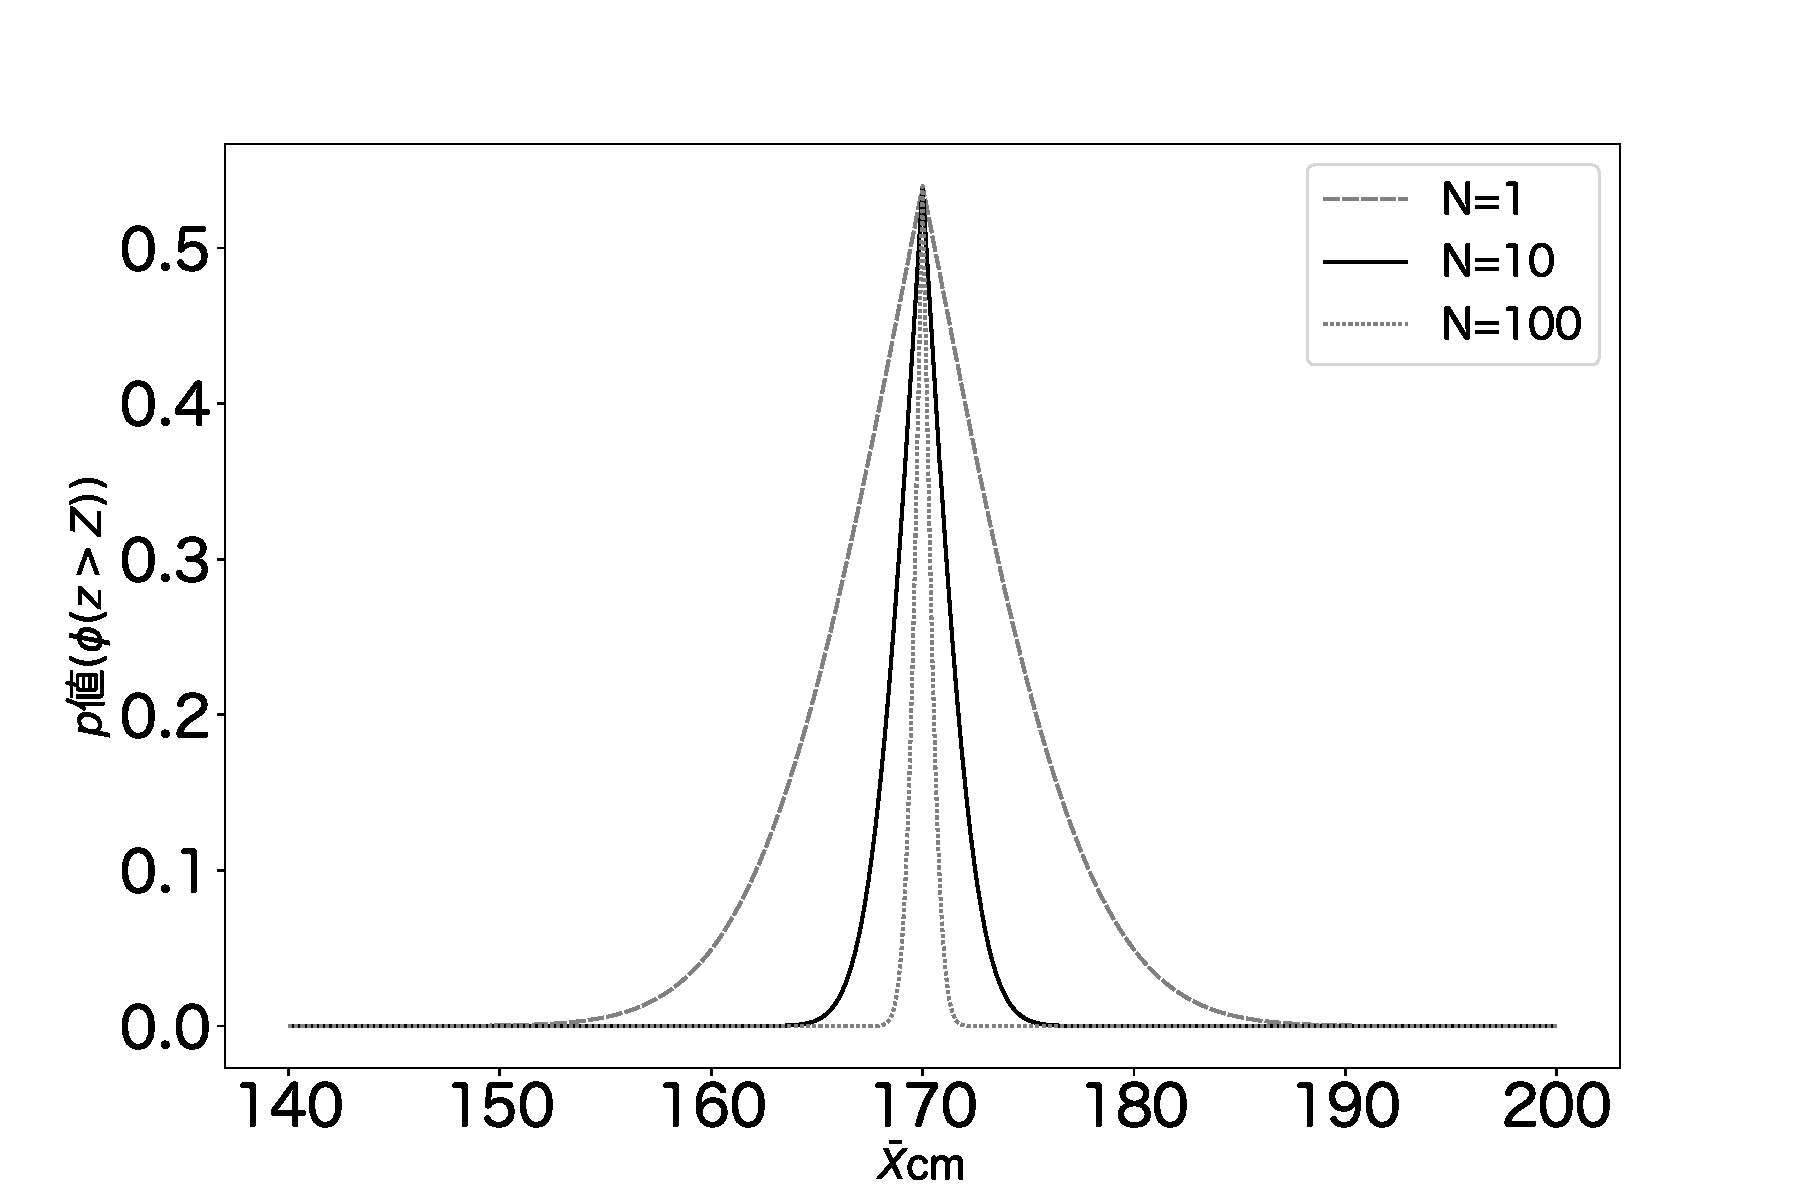
\includegraphics[width=15cm]{../markdown/section1/p_cm.pdf}
   %\caption{図1.p値cm}
 \end{center}
\end{figure}



 \if 0 

このとき、$Z(\bar{x},\mu)$が$N(0,1)$においてよくある値でない場合に、棄却します。
一方で、$Z(\bar{x},\mu)$が$N(0,1)$においてよくある値だったとしても、統計モデルを採用するとは言いません。
また、$Z(\bar,\mu)$の絶対値が$0$よりも十分大きな値を取れば、$N(0,1)$において出にくいということがわかります。これは、$|\bar{X}-\mu|$つまり、統計モデルの母数$\mu$と平均値$\bar{X}$の絶対値が大きければ、$Z(\bar{X},\mu)$の出現頻度は低く、絶対値が十分$0$に近ければ、$Z(\bar{X},\mu)$の出現頻度は高いことを意味します。

ここまでは、全て数学的フィクションである統計モデルの話をしました。では、現実のデータが
では、p値が語っていることを考えるいきます。


以上のことから、この検定を使うには、少なくともQ-Qプロットが必要であることが分かります。


一般に、統計モデルが棄却されない母数の領域を信頼区間といい、棄却される母数の領域を棄却区間という。
特に、$p=0.05$を基準とし、その基準における統計モデルが棄却されない区間を$95\%$ ($100*(1-0.05)$)信頼区間という。


信頼区間と対応する言葉として、採択域(棄却域)というものがある。棄却域は、確率変数を標準正規分布へ変数変換した後での信頼区間である。これは明らかに信頼区間と一対一対応する。

https://twitter.com/genkuroki/status/1270179975195316224


信頼区間は、データによって棄却されない母数の範囲のことである。

信頼区間は、統計モデルが棄却されるパラメータかどうかを表しているので、現実の推論を全く行っていない。

身長を統計モデルにより扱うことで、$p<0.05$では帰無仮説が棄却され、推測を行う統計モデルとはいまいちだということは分かったと思う。一方で、$p>0.05$となった場合でも積極的に採択しないことはなぜだろうか。次は、その理由を探る。
\fi
\subsubsection{統計モデルを積極的に採用しない理由}
設定した$\alpha=0.05$よりも大きな$p$値をもつ統計モデル$M(162.2)$は、それなりに推測するでしょうか。この統計モデルにより$P(x=170)$は、極めて少数であり、サンプルサイズを大きくしたときと乖離していることが分かります。このことから、全ての現象に対して特定の$p$値を元に棄却するモデルを決めることの無意味さを感じることができます。

p値が小さいとき、統計モデルの少なくとも一つの仮定と実際のデータとが合わないことが考えられます。そこでまず、統計モデルの仮定を満たしているのかを確認します。統計モデルの仮定(1)を確認します。身長データを無作為抽出して計測したため、身長データはそれぞれ独立であると考えられます。次に統計モデルの仮定(2)です。これは、Q-Qプロットを使います。もし、データが正規分布ではなさそうであれば、この統計モデルは使えません。
以上のことが確かめられたら統計モデルの仮定(3)が実際のデータと異なると結論付けます。少なくとも、ある母数では実際のデータと乖離していると主張するわけです。



実際に、検定を行なっておく。$N=1,\bar{x}=181$とする。このとき、$\bar{x}\sim N(\mu,\sigma^2)$より、$\frac{\sqrt{n}(170-\bar{x})}{\sigma}=-1.61$より、$z_{0.975}=-2.241$なので、棄却域に含まれない。統計モデル$M(170)$は棄却されない。
$N=4,\bar{x}=181$とする。このとき、$\frac{\sqrt{n}(170-\bar{x})}{\sigma}=-3.23$より、棄却されることがわかる。

棄却されるモデルが観測されたデータの平均値$\bar{x}$に応じて変化することを視覚的に確認しておく。図はさまざまな$\bar{x}$を得たときにその信頼区間を描いたものである。この信頼区間の範囲内にある$\mu$であれば、統計モデル$M(\mu)$は棄却されない。例えば、$\bar{x}=170$であれば、$M(170)$は棄却されない。一方で、$\bar{x}=165$あたりであれば、その棄却域は$\mu=170$を含まないので、$M(170)$は棄却される。

\begin{figure}
\begin{center}
    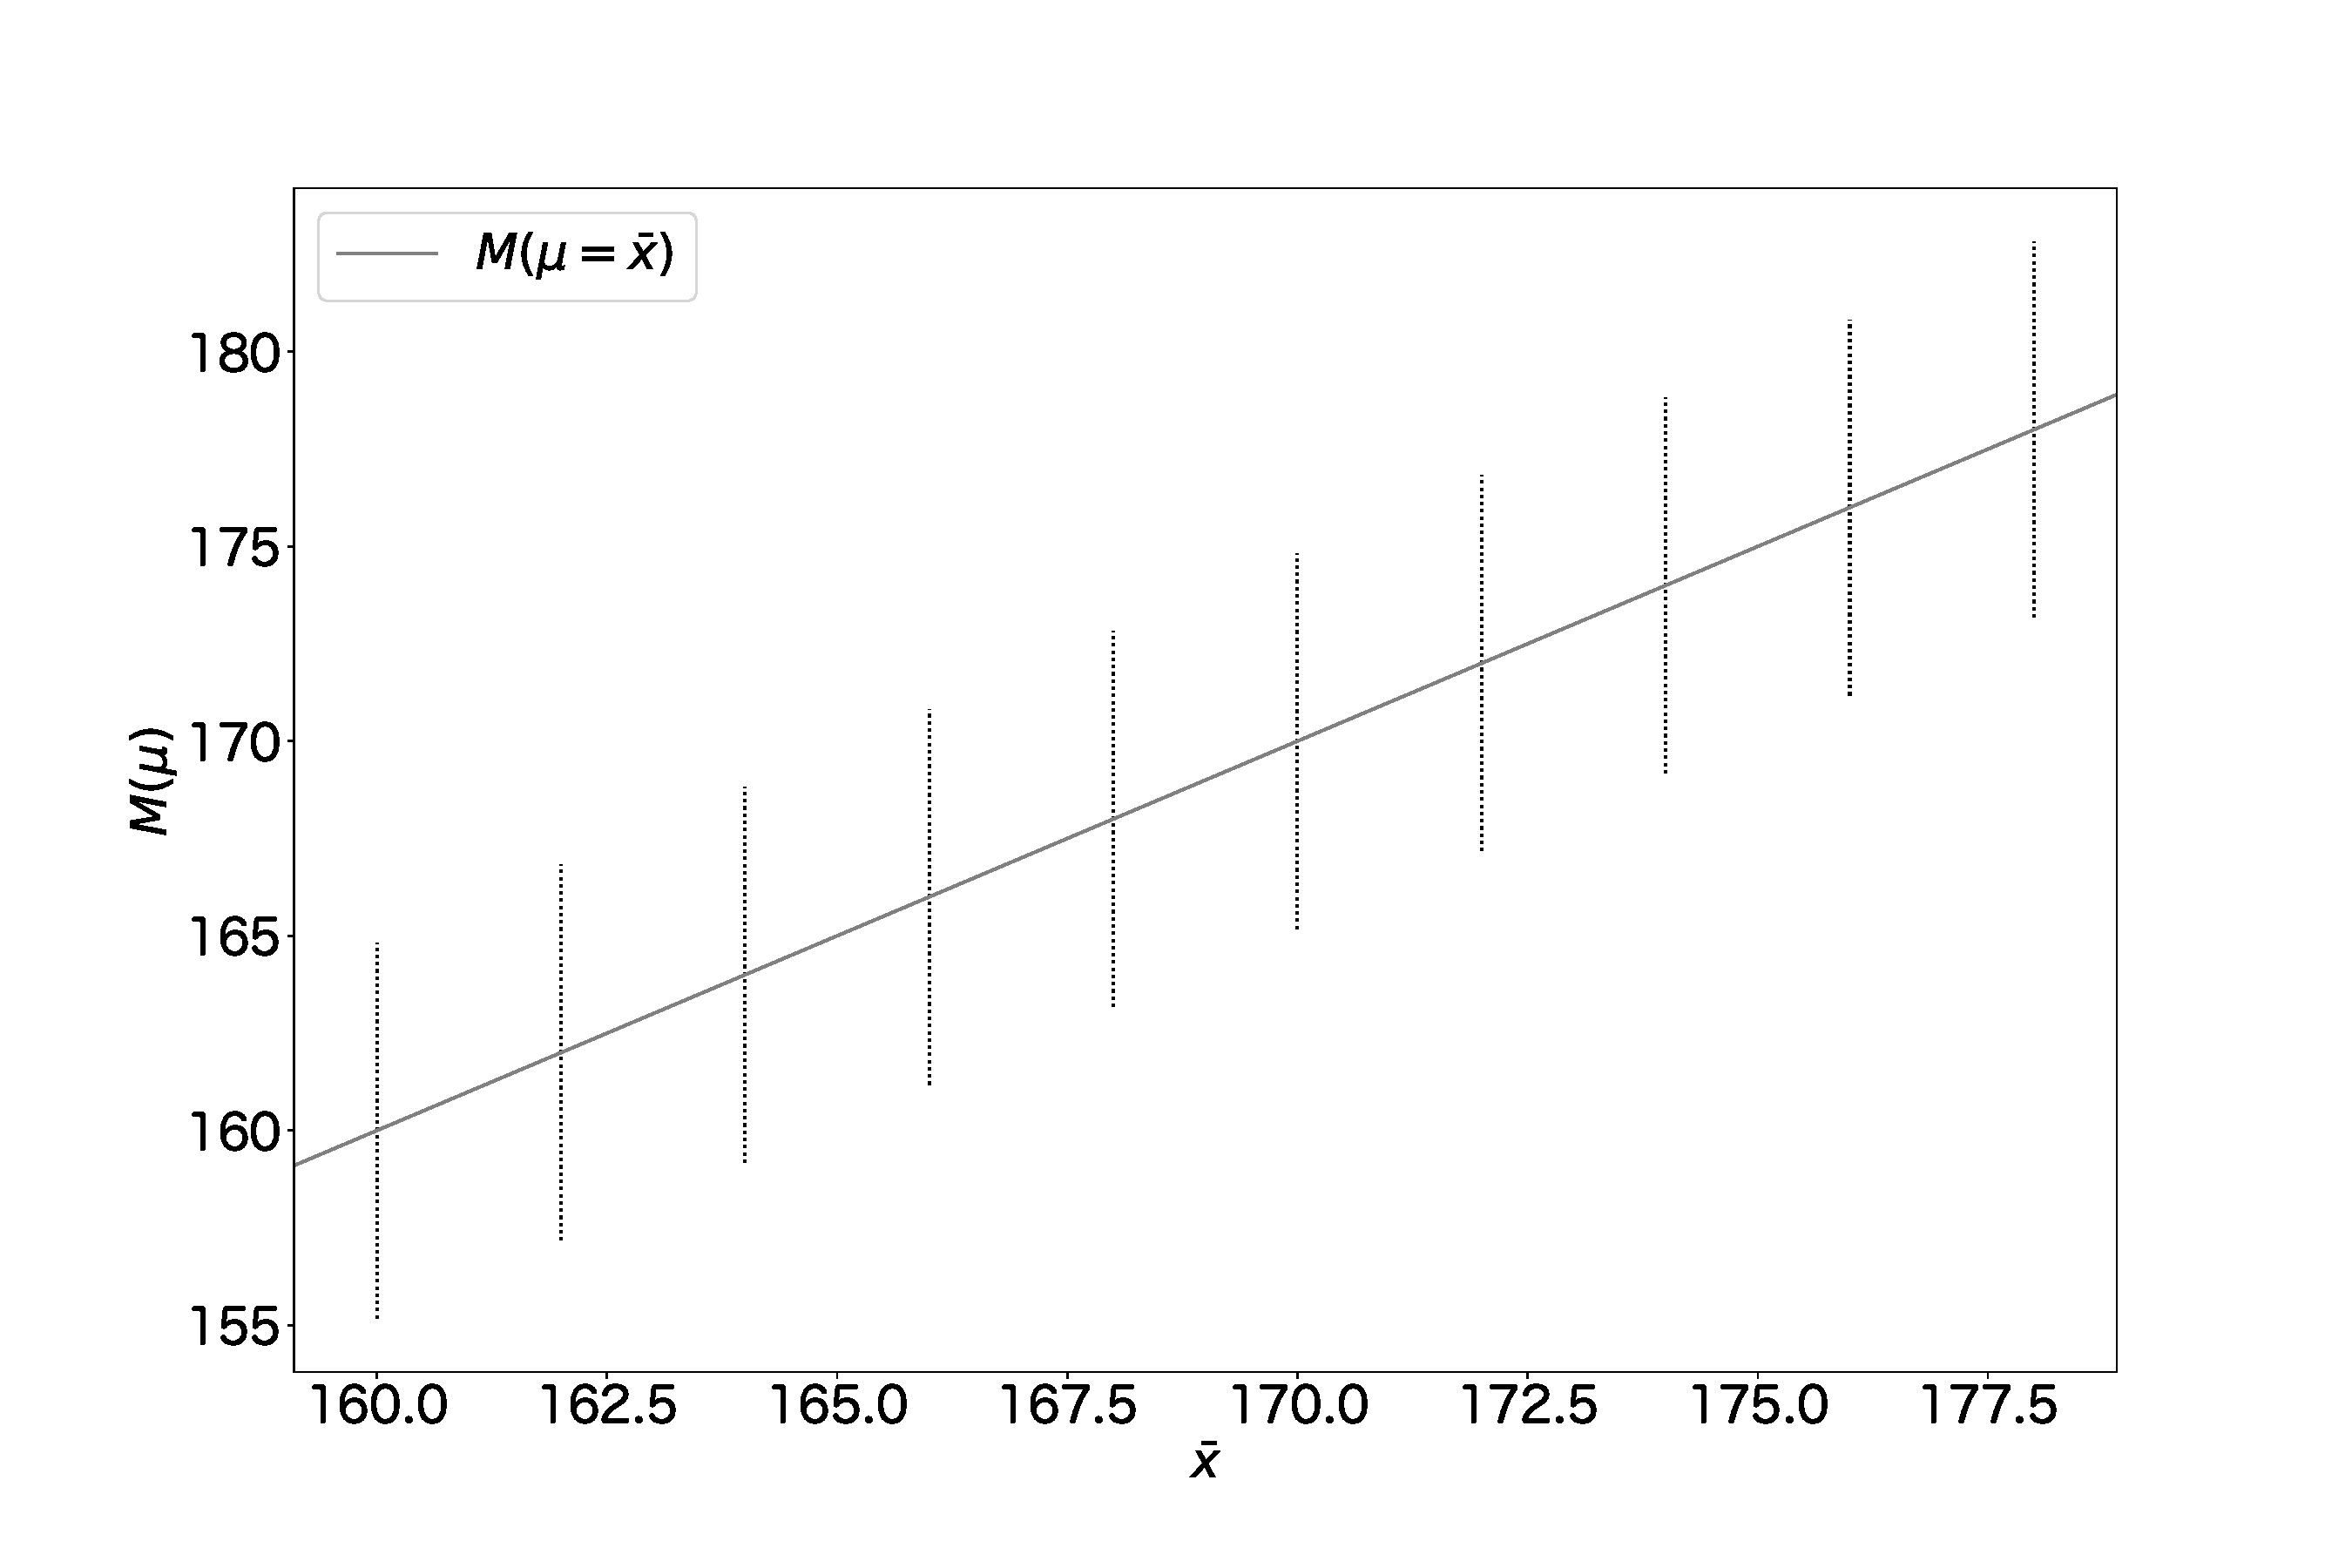
\includegraphics[width=15cm]{../markdown/section1/confidence_interval_model.pdf}
    %\caption{x軸は観測されたデータの平均値、y軸はモデルの母数$\mu$。}
  \end{center}
\end{figure}

\subsubsection{統計的仮説検定}
仮説検定はこれまで行ってきた統計モデルに対するモデルとの乖離を、たった一つの母数を対象に調べる方法です。
具体的には、データがある特定の母数$\mu$をもつ統計モデルの信頼区間に含まれるか否かによって、統計モデルが棄却されるかを調べます。
一般に、統計モデルの否定したい母数$\mu_0$を帰無仮説と言い、その母数ではないという$\mu\neq\mu_0$を対立かせつと言います。つまり、次のように帰無仮説を含む統計モデル$M_0$を構築します。
\begin{itemize}
    \item i.i.d
    \item 数学関数
    \item 統計モデルの母数を$\mu$とし、$\mu=\mu_0$
\end{itemize}
一番最後の仮説が帰無仮説と言います。
対立仮説を含む統計モデル$M_1$は、$M_0$と同様の仮説(1),(2)から構成されますが、仮設3は統計モデル$M_0$と$M_1$で異なります。
\begin{itemize}
    \item i.i.d
    \item 数学関数
    \item 統計モデルの母数を$\mu$とし、$\mu\neq\mu_0$
\end{itemize}
一番最後の仮説が対立仮説です。$M_1$の最後の仮説は、$M_0$の最後の仮設の否定系になります。

二つの統計モデルを作って、$M_0$で計算される信頼区間に、データから得られる統計量が入らないなら、$M_0$は棄却されます。逆に、統計量が信頼区間に入るなら、何も起こりません。
このように、否定したい仮説を設定し、少なくとも帰無仮説を含む統計モデルはだめだったと判断します。

\subsubsection{統計的仮説検定の手順}
統計的仮説検定の手順を確認します。
\begin{framed}
    \begin{enumerate}
        \item 過去の実験事実または予備実験から、無作為抽出したサンプルの出現頻度を予測する分布関数を特定する。ある点を中心に対称にデータが分布するのか、または、左右非対称にデータが分布するなどの知識・経験があったほうが良い。分布関数が全くわからないなら、正規分布を仮定する。
        \item その分布関数を含んだ統計モデルを構築する。統計モデルは以下の仮説から成り立つ。
        \begin{quote}
            \begin{itemize}
                \item 確率変数は独立同一分布に従う
                \item 分布関数
                \item 分布関数の母数がある値を取る
            \end{itemize}
        \end{quote}
        \item 統計モデルに母数を設定する.経験的に知っている値や、過去の論文や予備実験で明らかになった値である方が良い
        \item 統計モデルからサンプリングした確率変数の統計量が従う分布関数を探す。統計モデルの性質によって、母集団から得られた標本から得られた統計量の出現確率が計算可能になる。一般の統計検定ユーザーは本などでこの分布関数を確認する。
        \item 有意水準$\alpha$を設定する(さまざまな業界で$0.05$が設定される)。
        \item 母集団から無作為抽出を行い、標本を得る
        \item 標本が統計モデルにより推測できるかをもう一度考える。標本が統計モデルにより推測できること(標本の分布関数と統計モデルの分布関数がある程度一致している)、i.i.dであると考えることができるか。
        \begin{quote}
            標本が統計モデルにより推測できないと思われる場合、分布関数を変更し、統計モデルを再構築する。

            または、母集団の性質が別の分布関数になったのだから、統計検定を使うまでもなく、変化があったことが主張可能である。例えば、正規分布で推測できると(過去の実験や研究結果から)思われてたデータが、実際には指数分布的だった場合など。この場合、計測機器・無作為抽出の方法などに異常がなかったかも確認すべきである。
        \end{quote}
        \item 標本が統計モデルによりよく推測できるなら、その統計量もなんらかの分布関数に従っているはずであると考えられる。標本から統計量を計算し、統計モデルの中で、その統計量がその値以上に大きな値をとる確率を計算する($p$値)。
        \item $p$値が$\alpha$以下であれば、統計モデルの仮説の中の少なくとも一つの仮説が現象と乖離していると考える。
        \item 仮説(1)のi.i.dと、仮説(2)の分布関数とが、計測事実と大きく乖離がないならば、設定した母数が現実を上手く推測できていないと考える。このとき、帰無仮説を含む統計モデルは絶対にだめなモデルと判断する。一般に、帰無仮説が棄却されると宣言する。統計モデルと現実に乖離があるなら、そのことを宣言するべきである。
        \item $p$が$\alpha$以上であっても、積極的に推測に使えるとは言わない。一般に対立仮説を採用するとは宣言しない。
    \end{enumerate}
\end{framed}


この手順を身長の検証をするためになぞってみます。
\begin{enumerate}
    \item 普段の観察から、身長はある平均値の周りに対象に分布していることがなんとなくわかっているので、対象な分布関数の中から関数を選ぶ。また、サンプルサイズが大きいときの標本を見ると、正規分布でよく推定できることが知られている。以上のことから、正規分布で推測を試みる。
    \item 次の統計モデルを構築する。
    \begin{quote}
        \begin{itemize}
            \item 確率変数は独立同一分布に従う
            \item 正規分布関数
            \item 正規分布関数の母数$\mu,\sigma=5.7$
        \end{itemize}
    \end{quote}
    \item $\mu=170$
    \item 次のことがわかっている$x_1,\cdots,x_n$が正規分布$N(\mu,\sigma^2)$に従う確率変数であるならば、$\frac{\bar{x}-\mu}{\frac{\sigma}{\sqrt{n}}}\sim N(0,1)$である。ここで、$\bar{x}=\frac{x_1+x_2+\cdots+x_n}{n}$
    \item $\alpha=0.05$
    \item 母数からサンプルをランダム抽出し、標本とする。
    \item 無作為抽出できていかたと、標本を正規分布で推測しても良さそうかを検証する
    \item 標本の平均$\bar{X}$を計算し、統計モデルでの出現頻度を計算する。
    \item $p<\alpha$ならば、統計モデルの仮定のうち少なくとも一つがデータと乖離していると考える
    \item 仮説(1),仮説(2)はそれほど悪くない仮説であると思われるので、母数に関する仮定が間違っていると考えられる。以上から、母数は$\mu$ではないと宣言する。
\end{enumerate}

もしも、予備実験から実験状況に変化がなければ、帰無仮説を含んだ統計モデルは棄却されにくい。実験状況に変化があれば、帰無仮説を含んだ統計モデルは棄却されやすくなる。

\subsubsection{他の書籍との対応}
一般の生物学の教科書には、以上の手順の一部が省略して書かれている。これは、特定の分布関数にデータが従っていることを前提にしているからであるが、そのようなケースは実際の現象においては非常に稀であると考えられる。ゆえに、データと想定した統計モデルの違い・一致を注意深く検証しながら、統計的仮説検定を利用することが求められる。
%統計モデルがデータと乖離していれば、推定値が何を意味するかが捉えられなくなるので、統計モデルの改訂を要求されることもある。
%ただし、$p$値を小さくすることを目標に統計モデルを改訂してはいけない。
\begin{framed}
    \begin{itemize}
        \item 帰無仮説($\mu = \mu_0$)・対立仮説($\mu\neq \mu_0$)を設定する(上記の1-3)。
        \item 仮説が正しいと考えたとき、検定統計量従う分布を考える(4)。
        \item $\alpha$を設定する。(5)
        \item 母集団からの無作為抽出により標本を得る。(6)
        \item 検定統計量を計算し、その出現する確率$p$値を計算する。それが$\alpha$以下であれば、$\mu=\mu_0$ではないと結論づける(帰無仮説が棄却された。)(7-10)
    \end{itemize}
\end{framed}




\begin{mybox}
    \begin{quotation}
\paragraph{正規分布を前提にできる場合}
TODO:意味不明\\
非常に限定された条件で、標本が正規分布していることを前提として使えます。具体的には、標本が分布関数(Cauchy分布は当てはまらない)により生成されていることが前提となる場合です。このとき、中心極限定理によって、十分なサンプルサイズがある場合には、データが正規分布に近づきます。
言い換えれば、サンプルサイズを増やしていけば任意に小さな$p$値を得ることができます。
一方で、一般の現象は特定の分布関数によってデータが生成されているとは言うことはできません。この場合、正規分布に近づくことが正当化できる科学理論はありません。     
    \end{quotation}
\end{mybox}


\begin{mybox}
    \begin{quotation}
    \paragraph{偶然の差が生じたかを確かめたい}
    「偶然の差が生じたかを確かめたい」や「こんなことが起こる確率は$5\%$くらい」という言葉を統計学の教科書で見たことがあると思います。これはそれぞれ、「統計モデルの上で統計検定量が現れる確率が十分小さいことを確かめたい」や「統計モデル上でそのような統計検定量が得られる確率が$5\%$」を省略して書いたものです。
    
    統計学では、実験で得られたデータは、同様の実験を行った場合、同様のものが得られるということが要求されます。このことを現象に再現性があると言います。再現性のないデータを現状の統計学で扱うことはかなり難しい課題であり、現実の現象が得られる確率を議論することは困難です。
    \end{quotation}
    \end{mybox}
    
    
    \begin{mybox}
    \begin{quotation}
    \paragraph{帰無仮説のもとで偶然には起こり得ないことが起こった}
    帰無仮説のもとで偶然には起こり得ないことが起こったと言うふうに書くと、現実に起こりにくいと言うふうに印象付けられてしまう。非現実である統計モデルの上で、実験で得られた統計量以上の値が得られる確率は十分小さいと言い換えた方が良い。
    \end{quotation}
    \end{mybox}
    

\subsection{検出力}
母数の異なる二つの統計モデル$M_a,M_b$について考察する。母数から標本を得て、それぞれの統計モデルを統計量を元に評価する。
\subsubsection{検出力の定義}
$M_a$を棄却する判断をする閾値は、言い換えると、統計モデル$M_a$の棄却される母数(棄却域$R$)の出現確率を$\alpha$と言った。
また、$M_a$の棄却できない母数の範囲(信頼区間$A$)に$M_b$の統計量が存在する確率を$\beta$とする。$\beta$を検出力という\footnote{検出力を検定力または統計力と呼ぶこともある。\url{https://id.fnshr.info/2014/12/17/stats-done-wrong-03/}}。
$\alpha$は統計モデルとデータを比較したとき、そのモデルを棄却する指標である。
$\beta$は、二つの異なるモデルを比較するための指標で、一方のモデルで棄却できない母数がもう一方のモデルで出現する確率である。
$M_a$に対する$M_a$の検出力は、$1-\alpha$であり、$M_a$を棄却する閾値を低く設定すると、$\beta$は大きな値になる。
二つの統計モデルの母数がよく一致するならば、$\beta$は$1-\alpha$に近い値を取り、一致していないならば、$\beta$は0に近い値を取る。
具体的に、式で書くと、
\begin{eqnarray*}
    P_a(\mu \in R_a) = \alpha\\
    P_b(\mu \in A_a) = \beta
\end{eqnarray*}
ここで、$R_a,A_a$はそれぞれ統計モデル$M_a$の棄却域、信頼区間、$P_a,P_b$は、それぞれ統計モデル$M_a,M_b$における統計量の確率密度関数。

\subsubsection{正規分布モデルの検出力}
具体的に、$P_a(\mu \in R_a),P_b(\mu\in A_a)$を計算してみる。
正規分布を含む統計モデルを構築する
\begin{quote}
    \begin{enumerate}[(1)]
\item i.i.d
\item $N(\mu,\sigma^2)$
\item 母数$\mu$,$\sigma$は既知とする(一般性を持たせるために、具体的な値は書かない。$\sigma=1$と読み替えて進めても良い)
\end{enumerate}
\end{quote}
このモデルを$M(\mu)$とし、$M_a=M(\mu_a),M_b=M(\mu_b)$とする。
$M_a$または、$M_b$からサンプリングされた確率変数$x_1,x_2,\cdots,x_n$の平均値は、それぞれ$\bar{x}_a\sim N(\mu_a,\sigma/n)$または$\bar{x}_b\sim N(\mu_b,\sigma/n)$である。
$M_a$の信頼区間$A_a$は、$|\bar{x}_a|<\mu_a+\sigma / \sqrt{n}z_{2.5\%}$である。
このとき、$P_a$を$N(\mu_a,\sigma)$の確率密度関数とすると、
\begin{equation*}
    P_a(\mu \in A_a) = \alpha
\end{equation*}
であるのは定義から明らか。
また、$P_b$を$N(\mu_b,\sigma)$の確率密度関数とすると、
\begin{equation*}
    P_b(\mu \in A_a ) = \beta
\end{equation*}
である。
$\mu_a$と、$\mu_b$が一致していれば、$P_b(\mu \in A_a ) = 1-\alpha$である。
$\mu_b$が$\mu_a$から離れていくと、$P_b(\mu \in A_a)=0$に近づいていく。


\begin{figure}
\begin{center}
    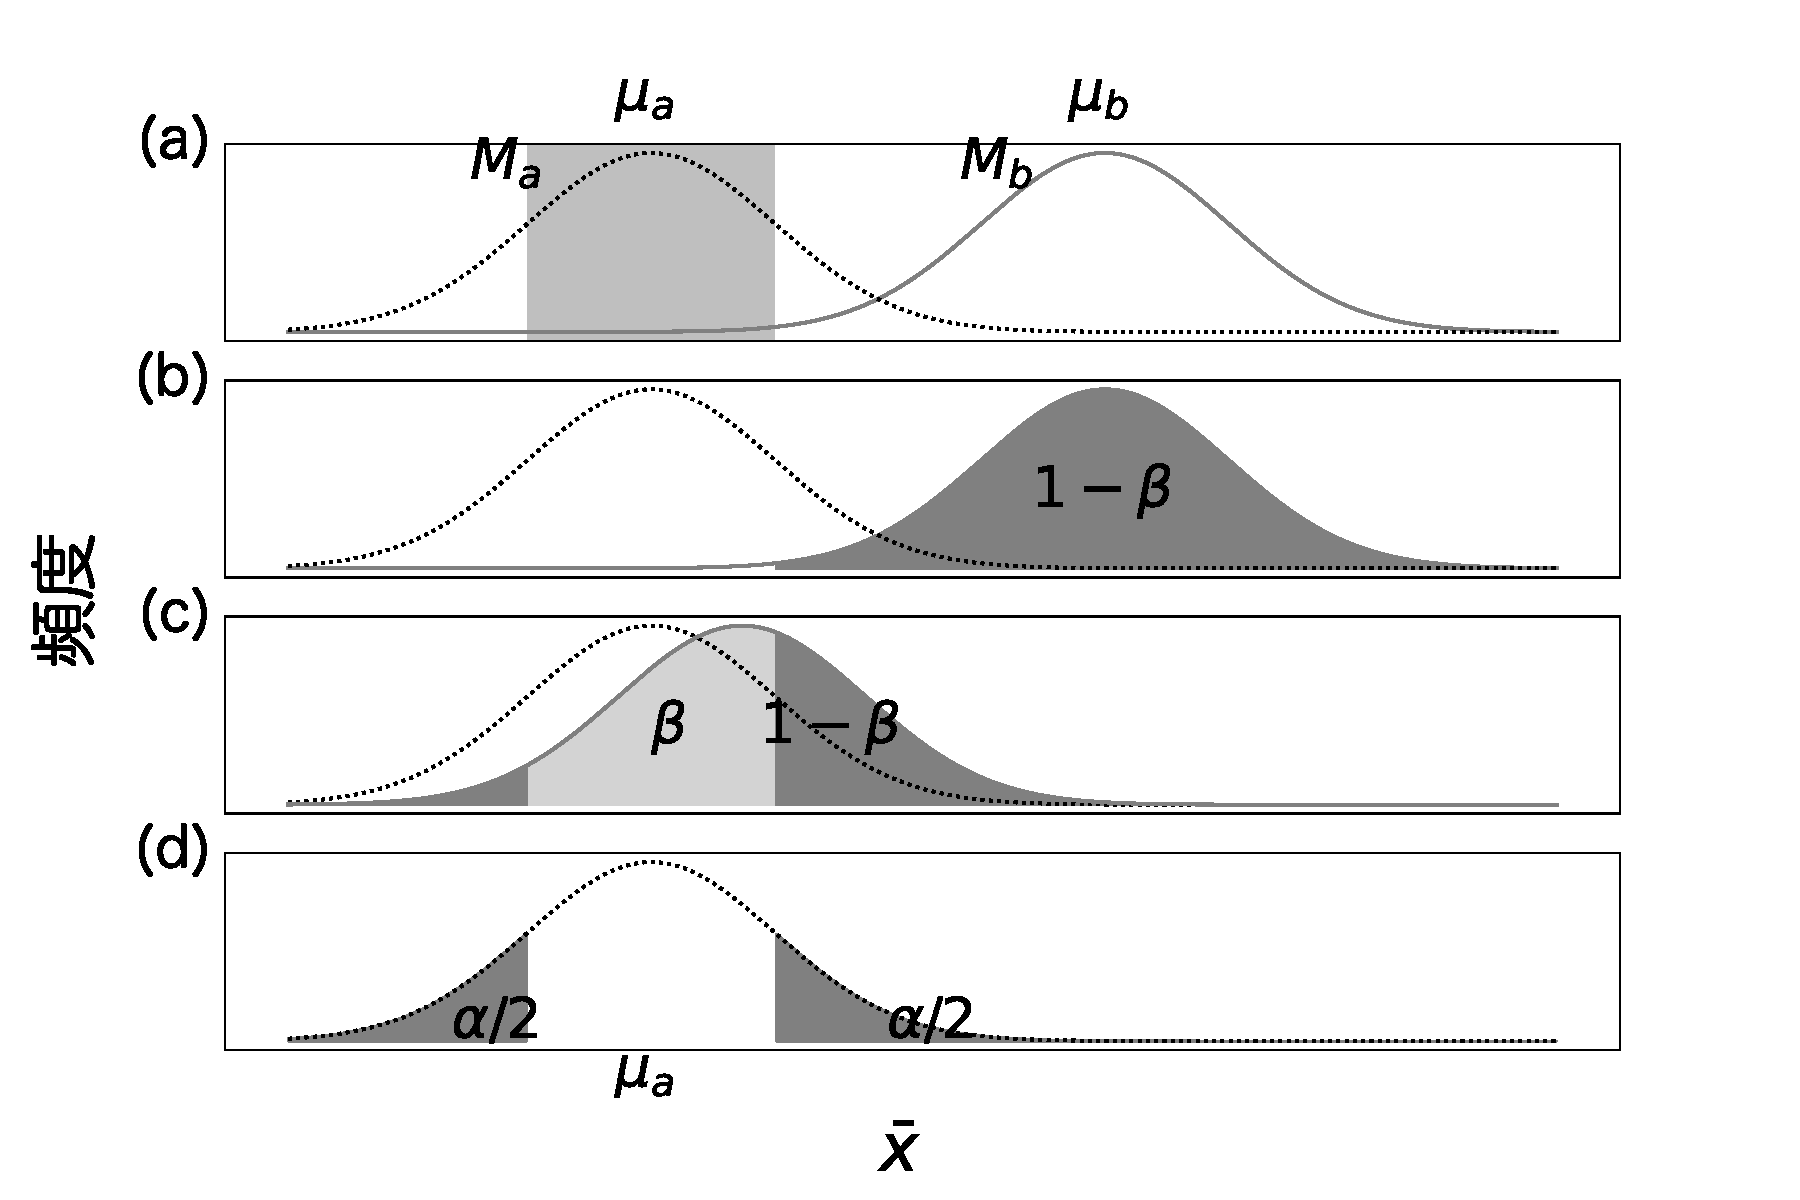
\includegraphics[width=15cm]{../markdown/section1/power_of_a_test_2.pdf}
    \caption{統計モデル$M_a,M_b$から計算された統計量$\bar{x}$の確率分布$P_a,P_b$。(a)灰色の範囲は$M_a$の信頼区間。(b)灰色の領域は、$1-\beta$の領域を示している。$\beta$の領域が小さいので、描画できなかった (c)$\mu_b$が$\mu_a$に近いときの$\beta$と$1-\beta$の領域。(d)灰色の範囲の面積が$\alpha$を示している。}
    \label{fig:power_of_test_alpha_beta}
\end{center}
\end{figure}


検出力と$\alpha$の領域を図示した(図\ref{fig:power_of_test_alpha_beta})。$M_a$の$95\%$信頼区間は、$|\mu|<\mu_a+z_{0.025}\frac{\sigma}{\sqrt{N}}$である。信頼区間は、図\ref{fig:power_of_test_alpha_beta}(a)において灰色で塗った$x$軸の範囲である。$\alpha$は図\ref{fig:power_of_test_alpha_beta}(c)の灰色で塗りつぶした領域の面積である。
検出力$1-\beta$は、$M_b$における$M_a$の信頼区間の外側の領域の面積なので、図\ref{fig:power_of_test_alpha_beta}(b)の濃い灰色の範囲である。

$\alpha$を0に近づけていくと、信頼区間は徐々に大きくなり、$\beta$は大きくなる。
$\alpha$を1に近づけていくと、信頼区間は徐々に狭くなり、$\beta$は小さくなる。



\begin{figure}
    \begin{center}
        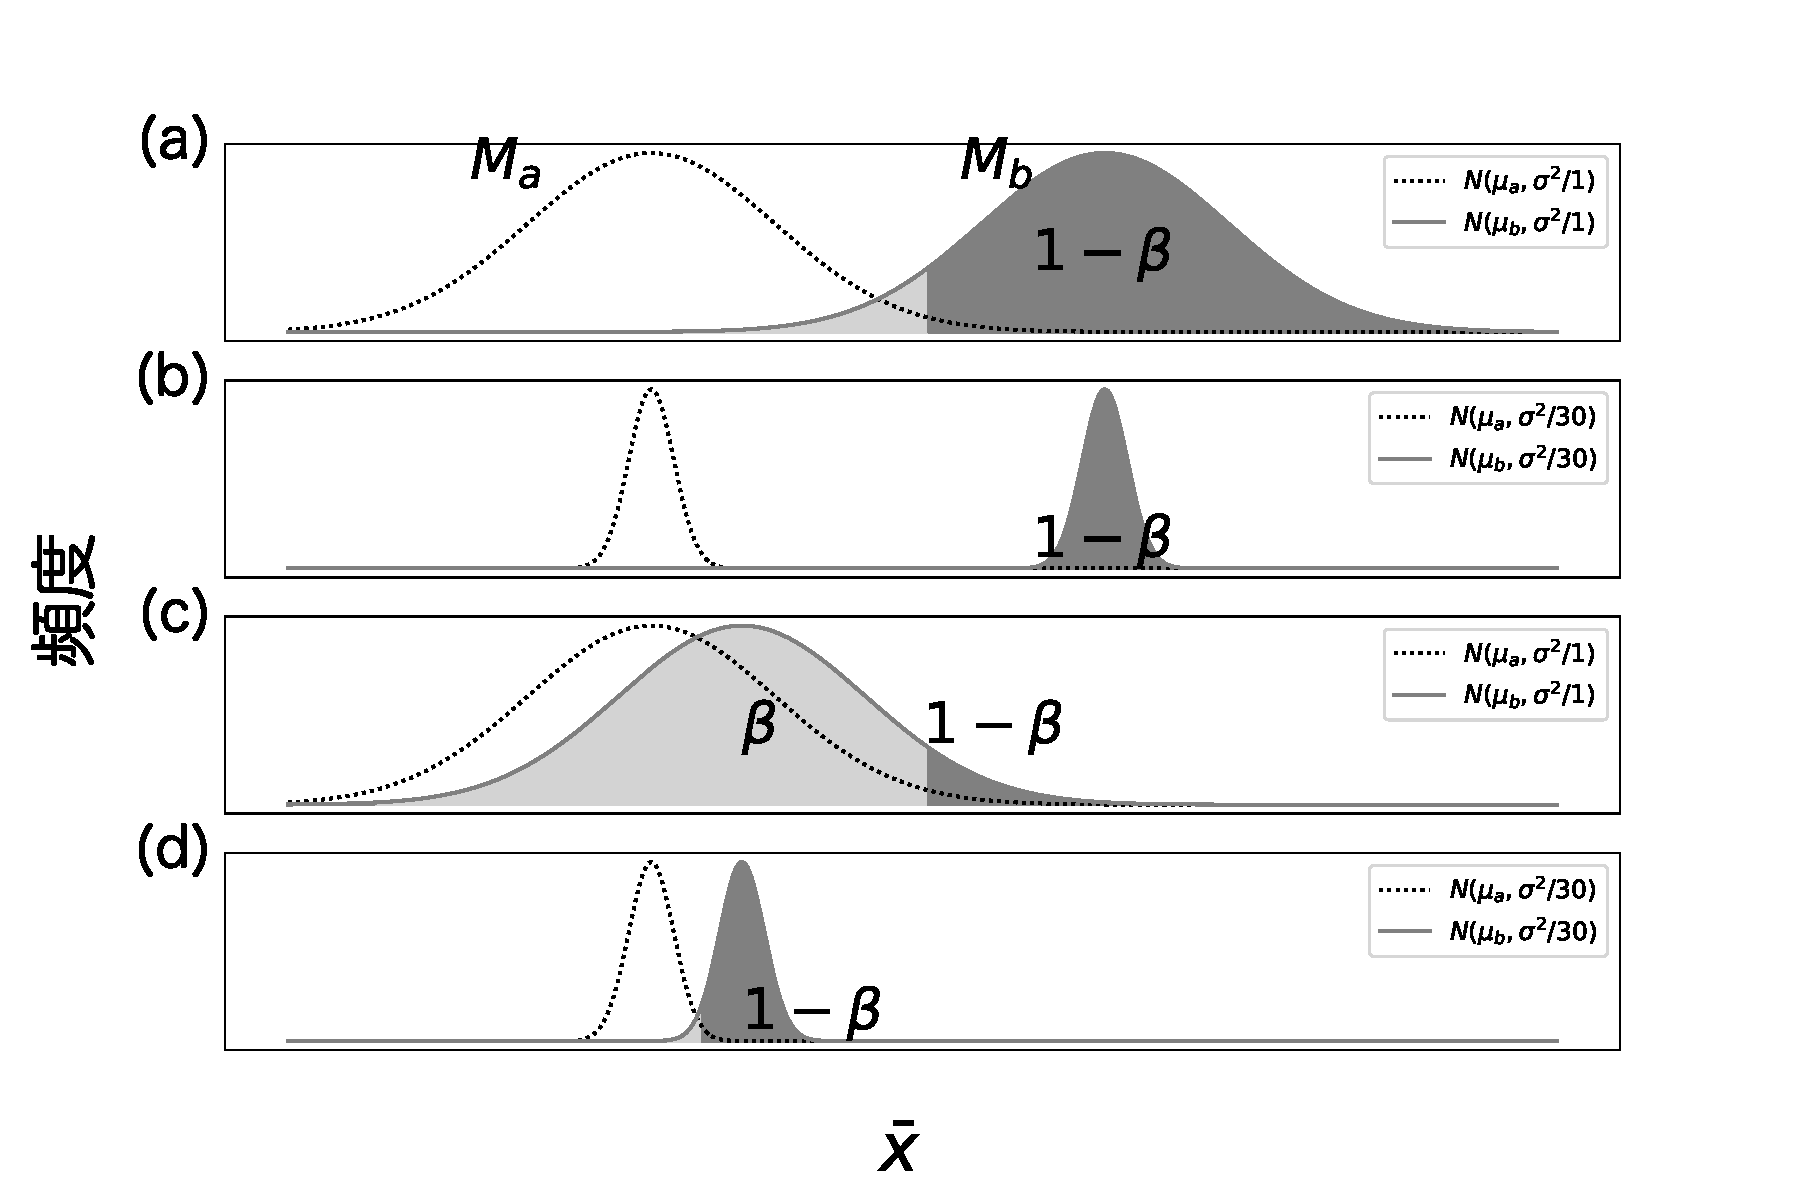
\includegraphics[width=15cm]{../markdown/section1/power_of_a_test_3.pdf}
        \caption{統計モデル$M_a,M_b$から計算された統計量$\bar{x}$の確率分布$P_a,P_b$。(a)$\mu_a,\mu_b$のサンプルサイズ$1$の平均値がしたがう確率密度関数$N(\mu_a,\sigma^2/1),N(\mu_a,\sigma^2/1)$。(b)(a)と同じ$\mu_a,\mu_b$に対して、サンプルサイズを$30$にした場合の確率密度関数。(c)$\mu_a,\mu_b$が(a)よりも近いときの$\bar{x}$の確率密度関数。(d)(c)と同じ$\mu_a,\mu_b$に対してサンプルサイズを$30$にした場合の$\bar{x}$の確率密度関数。}
        \label{fig:power_of_test_alpha_beta_sample_size}
    \end{center}
    \end{figure}

    

$\alpha$、$M_a$の母数$\mu_a$、$M_b$の母数$\mu_b$を固定したまま、サンプルサイズを変化させるときのことを考えてみる(図\ref{fig:power_of_test_alpha_beta_sample_size})。$\bar{x}$の確率密度関数($N(\mu,\sigma^2/n)$)の分散がサンプルサイズによって変化することは明らかである。このことから、サンプルサイズが大きくなると、信頼区間は徐々に狭くなり、$1-\beta$は大きくなる。サンプルサイズが小さいときは、$1-\beta$も小さくなる。

$\mu_a$を固定し、$\mu_b$を変化させたときの検出力$1-\beta$を図\ref{fig:power_of_test_N_mu0_variable}に示した。
サンプルサイズが大きければ、$1-\beta$も大きくなることがわかる。

\begin{figure}
    \begin{center}
        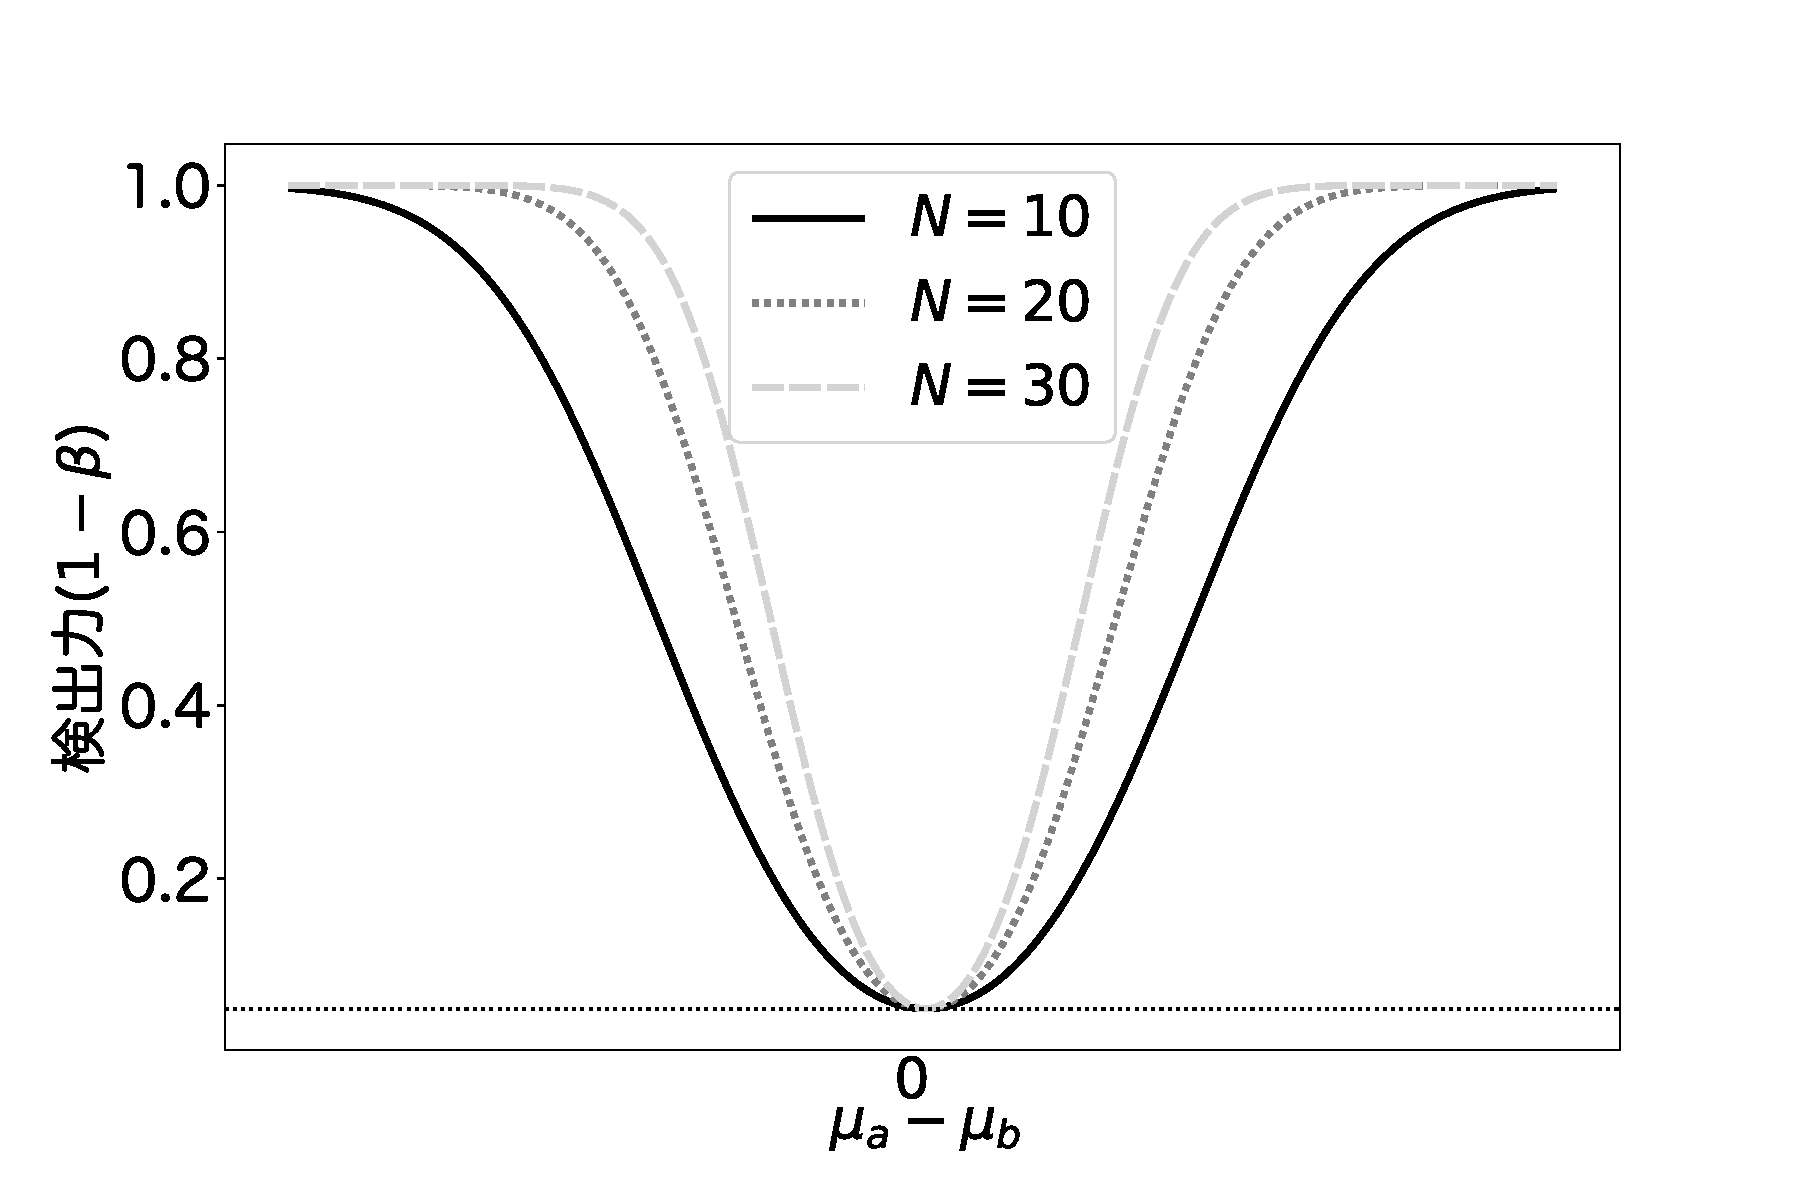
\includegraphics[width=15cm]{../markdown/section1/power_of_test.pdf}
        \label{fig:power_of_test_N_mu0_variable}
        \caption{$\mu_a$を変数にしたときの検出力(検出力関数)。}
    \end{center}
\end{figure}

$\beta$を定義したことにより、$M_a,M_b$の違いをはっきりさせるために必要なサンプルのサイズが計算できる。ここでは、$\mu_a,\mu_b$が固定されている状況を考える。
検出力$1-\beta$は$1$に近いほど、$M_a,M_b$が違うと主張できる。
あらかじめ決めたおいた基準の$1-\beta$を閾値を設定し、それ以上の$1-\beta$となるサンプルサイズを計算すれば良い。
サンプルサイズが小さければ、$M_a$と$M_b$の違いは曖昧であり、サンプルサイズが大きくなると、はっきりとモデルの違いがわかる。



\begin{mybox}
    \begin{quote}
    \paragraph{第一の過誤・第二の過誤・統計モデルが正しい}
        Neyman-Pearson流の統計学の方言においては、$\alpha,\beta$を次のように定義する。帰無仮説を含む統計モデルが正しいとき、誤ってそのモデルを棄却してしまう間違いを第一の過誤といい、この確率を$\alpha$とする。また、対立仮説を含む統計モデルが正しいのに、帰無仮説を採択する間違いを第二の過誤といい、この確率を$\beta$とする。

        Fisher流派とNeyman-Pearson流派の両方を同じように扱うことが問題視されている[\cite{published_papers/18436201}]。
        私は、ある統計モデルが正しいとは考えないので、「モデルが正しいとき、間違えてそのモデルを棄却する間違い」ということを考える流派に同意できなかった。
        統計モデルは棄却されることはあるが、正しいことや積極的に採択されることは稀であるというのはFisherの流派が近いように思う。
        ただし、Fisherは、「$p$値を帰無仮説が正しいという条件のもとで、手元にあるデータ、およびさらに極端なデータが得られる確率」と定義した[\cite{1573106361610039296}]。
        ここでの正しいという言葉の意図が重要である。
        私は、「統計モデルの仮説が自然を記述するのにほどほど良いと考えられるとき、手元にあるデータの統計量以上の隔たりが統計モデル内で得られる確率」という意味であると考えている。

        Neyman-Pearson流派の統計学の教科書を科学の分野で見つけることができていない。
        Fisher流派とNeyman-Pearson流派の両方を書いている教科書は存在しているが、「帰無仮説を含む統計モデルが正しい」とはどういうことかを答えたものを見つけることができていない。
    \end{quote}
\end{mybox}


\begin{mybox}
    \begin{quote}
    \paragraph{p値の多様な解釈}
$p$値は分野によって多様な解釈がなされることがある\cite{published_papers/18436201,2020医療統計解析使いこなし実践ガイド}。
\if 0
例えば、ASAの声明[\cite{ASA_JA}]を引用しているにもかかわらず、
$p$値は、証明したい仮説が真である場合、研究で行った前提条件が担保されている場合、研究で得られた結果が実際に得られる確率を示している\cite{2020医療統計解析使いこなし実践ガイド}。

などと書かれる場合がある。
ここで、「実際に得られる確率」が何を指しているのかが不明確であるが、「統計モデル上で実験で得られた統計量が得られる確率」を意図すると読み替えることはできるのだろうか。
\fi

よい解釈として以下の6つの原則が示されている\cite{published_papers/18436201}
\begin{enumerate}
    \item $p$値はデータと特定のモデルが矛盾する程度を示す指標の一つである。
    \item $p$値は調べている仮説が正しい確率や、データが偶然飲みで得られた確率を図るものではない。
    \item 科学的な結論や、ビジネス、政策における決定は$p$値がある値を越えたかどうかのみに基づくべきではない。
    \item 適正な推測のためには、全てを報告する透明性が必要である
    \item $p$値や統計的優位性は、効果の大きさや結果の重要性を意味しない。
    \item $p$値は、それだけでは統計モデルや仮説に関するエビデンスの、よい指標とはならない。
\end{enumerate}

    $p$値や信頼区間を報告することがASAの声明では求められている。私は、それら以外の情報として、ランダムサンプリングされているということ・再現可能性・正規分布を含んだ統計モデルなどを研究者がどの程度信じているのかということも報告するべきだと考えている。統計モデルの仮定が現象から著しく外れているのならば、統計モデルを使った推論は無意味である。
    また、研究者の統計学への心情がわかれば、報告に価値があることを理解しやすくなる。

    誤解とされる解釈はも引用しておく\cite{idiot_statistics2014}\footnote{原典は\cite{GOODMAN2008135}である。孫引き引用である}。
    \begin{enumerate}
        \item $p=0.05$ならば、帰無仮説が真である確率は$5\%$しかない。
        \item $p\geq 0.05$のような有意でない結果は、グループ間に差がないことを意味する
        \item 統計的に有意な発見は客観的に重要である
        \item $p$値が$0.05$より大きい研究と小さい研究は矛盾する
        \item $p$値が同じ研究は帰無仮説に対して同等の証拠を提供する。
        \item $p=0.05$は、帰無仮説のもとで$5\%$しか起こり得ないデータを観察したことを意味する
        \item $p=0.05$と$p\leq 0.05$は同じことである。
        \item $p$値は不等式の形で書かれるものである(例えば、$p=0.015$のときは$p\leq 0.02$とする)。
        \item $p=0.05$は、帰無仮説を棄却したとしたら、第一種の誤りの確率が$5\%$しかないことを示す。
        \item 有意水準$p=0.05$のもとで、第一種の誤りの確率は$5\%$になる。
        \item ある方向を向いた結果やその方向の結果があり得ない差異を気に留めないのであれば、片側の$p$値を用いるべきである。
        \item 科学に関する結果や処方の方針は$p$値が有意であるかどうかに基づくべきである。
    \end{enumerate}

    \end{quote}
\end{mybox}

\subsubsection{$\beta$の計算}
正規分布を含んだ統計モデル$M_a,M_b$を使って、$\beta$を計算してみる。
$M_a$の信頼区間は、
\begin{equation*}
    -z_{0.025}\leq \frac{\sqrt{n}(\bar{x}-\mu_a)}{\sigma}\leq z_{0.025}
\end{equation*}
より、
\begin{equation*}
    A_a = \{ \mu ; \mu_a -\frac{\sigma}{\sqrt{n}}z_{0.025} \leq \mu \leq \mu_a +\frac{\sigma}{\sqrt{n}}z_{0.025} \}
\end{equation*}
である。ここで、$a=\mu_a -\frac{\sigma}{\sqrt{n}}z_{0.025},b = \mu_a +\frac{\sigma}{\sqrt{n}}z_{0.025} $とおく。棄却域は$A_a$以外の$\mu$である。$M_b$の標本平均$\bar{x}_b$は、$N(\mu,\frac{\sigma^2}{n})$に従うので、$A_a$の区間で、$N(\mu_b,\frac{\sigma^2}{n})$の面積を計算すれば良い。
ここで、$\frac{\sqrt{n}(\bar{x}_b-\mu_b)}{\sigma}\sim N(0,1)$である。
このことを利用すると、
$a,b$は、$N(\mu_b,\frac{\sigma^2}{n})$の確率変数だとすると、
\begin{eqnarray*}
    A &=& \frac{\sqrt{n}(a-\mu_b)}{\sigma} \\
    &=& \frac{\sqrt{n}(\mu_a-\frac{\sigma}{\sqrt{n} z_{\alpha/2}})}{\sigma}\\
    &=& -z_{\alpha/2}+\frac{\sqrt{n}}{\sigma}(\mu_a-\mu_b)
\end{eqnarray*}
同様に、
\begin{eqnarray*}
    B &=& \frac{\sqrt{n}(b-\mu_b)}{\sigma} \\
    &=& \frac{\sqrt{n}(\mu_a-\frac{\sigma}{\sqrt{n} z_{\alpha/2}})}{\sigma}\\
    &=& z_{\alpha/2}+\frac{\sqrt{n}}{\sigma}(\mu_a-\mu_b)
\end{eqnarray*}
である。以上より、確率密度関数$N(0,1)$において、$-z_{\alpha/2}+\frac{\sqrt{n}}{\sigma}(\mu_a-\mu_b) \leq x\leq  z_{\alpha/2}+\frac{\sqrt{n}}{\sigma}(\mu_a-\mu_b)$の間で積分すれば良い。

$d=\frac{\mu_a-\mu_b}{\sigma}$とおく。$d=0.6,n=9$とする。このときの$\beta$を計算してみる。$N(0,1)$において、$-z_{\alpha/2} -0.6\sqrt{n} \leq x \leq z_{\alpha/2} +0.6\sqrt{n}$の区間で積分する。

\begin{lstlisting}
A,B = norm.interval(0.95,0.,1)
N = 9
d = 0.6
a,b = A+d*np.sqrt(N),B+d*np.sqrt(N)
print(a,b)
norm.cdf(b,0,1)-norm.cdf(a,0,1)
\end{lstlisting}

答えは、$0.564$

\subsubsection{データを元にしたモデルとモデルの類似度}
統計モデルAを$M(\mu=170)$とし、統計モデルBを$M(\bar{X})$とする。ここで、$\bar{X}$は、無作為抽出によって得られた標本の平均であり、標本の大きさを$100$とする。
モデルA,Bの間の検出力が計算可能である。
$d=\frac{170-\bar{X}}{6.8}$、$n=100$であるので、$\bar{X}=168$を得たとすると、
\begin{lstlisting}
A,B = norm.interval(0.95,0,1)
N = 100
d = (170-168)/(6.8)
a,b = A+d*np.sqrt(N),B+d*np.sqrt(N)
print(a,b)
norm.cdf(b,0,1)-norm.cdf(a,0,1)
\end{lstlisting}
その検出力は、$0.163$

\subsubsection{サンプルサイズ}
$d$と検出力を指定したときに、$M_a,M_b$の類似度を検出力以上にするためのサンプルサイズが計算できる。
$\beta=0.1,\d=0.8$とし、この$\beta$を満たすように$N$を計算した。

\begin{lstlisting}
A,B = norm.interval(0.95,0.,1)
beta = 0.1
d = 0.8
for N in range(10,200,2):
    a,b = A+d*np.sqrt(N),B+d*np.sqrt(N)
    beta_ = norm.cdf(b,0,1)-norm.cdf(a,0,1)
    if beta_ < beta:
        break
print(N)
\end{lstlisting}
計算を実行すると、$18$であることがわかる。


\subsection{第一の過誤}
統計モデルの中で、統計モデルを統計量により検査するときに、モデル自身を絶対にダメなモデルと判断してしまうことを第一の過誤(type I error)と言う。
この過誤は、2つの要因に分解すると\footnote{$\alpha_2$は$\alpha_1$に関係するので実際には、分解できない。}、不適切な統計量を使用することで、棄却域と統計量の違いにより生じる$\alpha_1$、そして、検定を繰り返して生じる$\alpha_2$である($0<\alpha_1+\alpha_2 \leq 1$)。
$\alpha_1+\alpha_2=\alpha$となっていれば、有意水準$\alpha$の検定ができる。
$\alpha_1$は、統計モデルと、その統計量の関数になっており、言い換えれば、統計モデルと統計量の適合度を測る指標である。
正規分布を含んでいる統計モデルを使い、統計量$T$を使った場合、$\alpha_1 \approx	 0 $であるが、指数分布を含んだ統計モデルを使い、統計量$T$を使った場合、$\alpha_1 > 0$となる。これを見ていく。
$\alpha_2$については、後で調べる。
$\alpha_2$は、$\alpha\times 2$以上になる場合、軽視されることはないが、
$\alpha_1$が同程度の隔たりになる場合においては無視され、$\alpha_1$は$\alpha_2$よりも軽視されがちである。
%統計モデルに対して不適切な統計量を使ってモデルの検証を試みると、第一の過誤が変化することがわかっている。

\subsubsection{どんな統計モデルでも$T$統計量で調べよう($\alpha_1$)}
統計モデルの分布の仮定が正規分布以外の場合においても、$T$統計量を使ってモデル自身を検証できるのかを調べる。次の統計モデル$M(\lambda)$を構築する。
\begin{enumerate}
    \item $X_1,X_2,\cdots,X_n $はi.i.d
    \item 指数分布
    \item $\lambda$
\end{enumerate}
母数$\lambda=1$とした統計モデルを$M(1)$とする。
$M(1)$からランダムサンプリングした確率変数$x_1,x_2,\cdots,x_n$から次の統計量を計算する。
\begin{equation*}
    T = \frac{\bar{X}-1}{\sqrt{\frac{\sigma^2}{n}}}
\end{equation*}
ここで、$T \sim t(n-1)$とする。
$T$値が$t(n-1)$の棄却域に入っている頻度を数値計算により計算する。
具体的に、平均$1$の指数分布または、平均$1$、標準偏差$1$の正規分布からサンプルを得て標本を作る。その標本を$100000$回取得する。
このとき、$T$値を計算し、$T$値いじょの値が得られる確率$p$を計算する。その$p$が$p<0.05$となる割合を計算する。以上をサンプルサイズを変化させてシミュレーションを行なった。
平均$1$、標準偏差$1$の正規分布の場合、$T$値は$t(n)$分布に従ので、$p<0.05$となる頻度も、$5\%$程度になることが期待される。
一方で、平均$1$の指数分布の場合、$T$は$t(n-1)$分布に従うとはいえない。このことから、$p<0.05$となる頻度は計算してみなければわからない。


\begin{figure}
    \begin{center}
        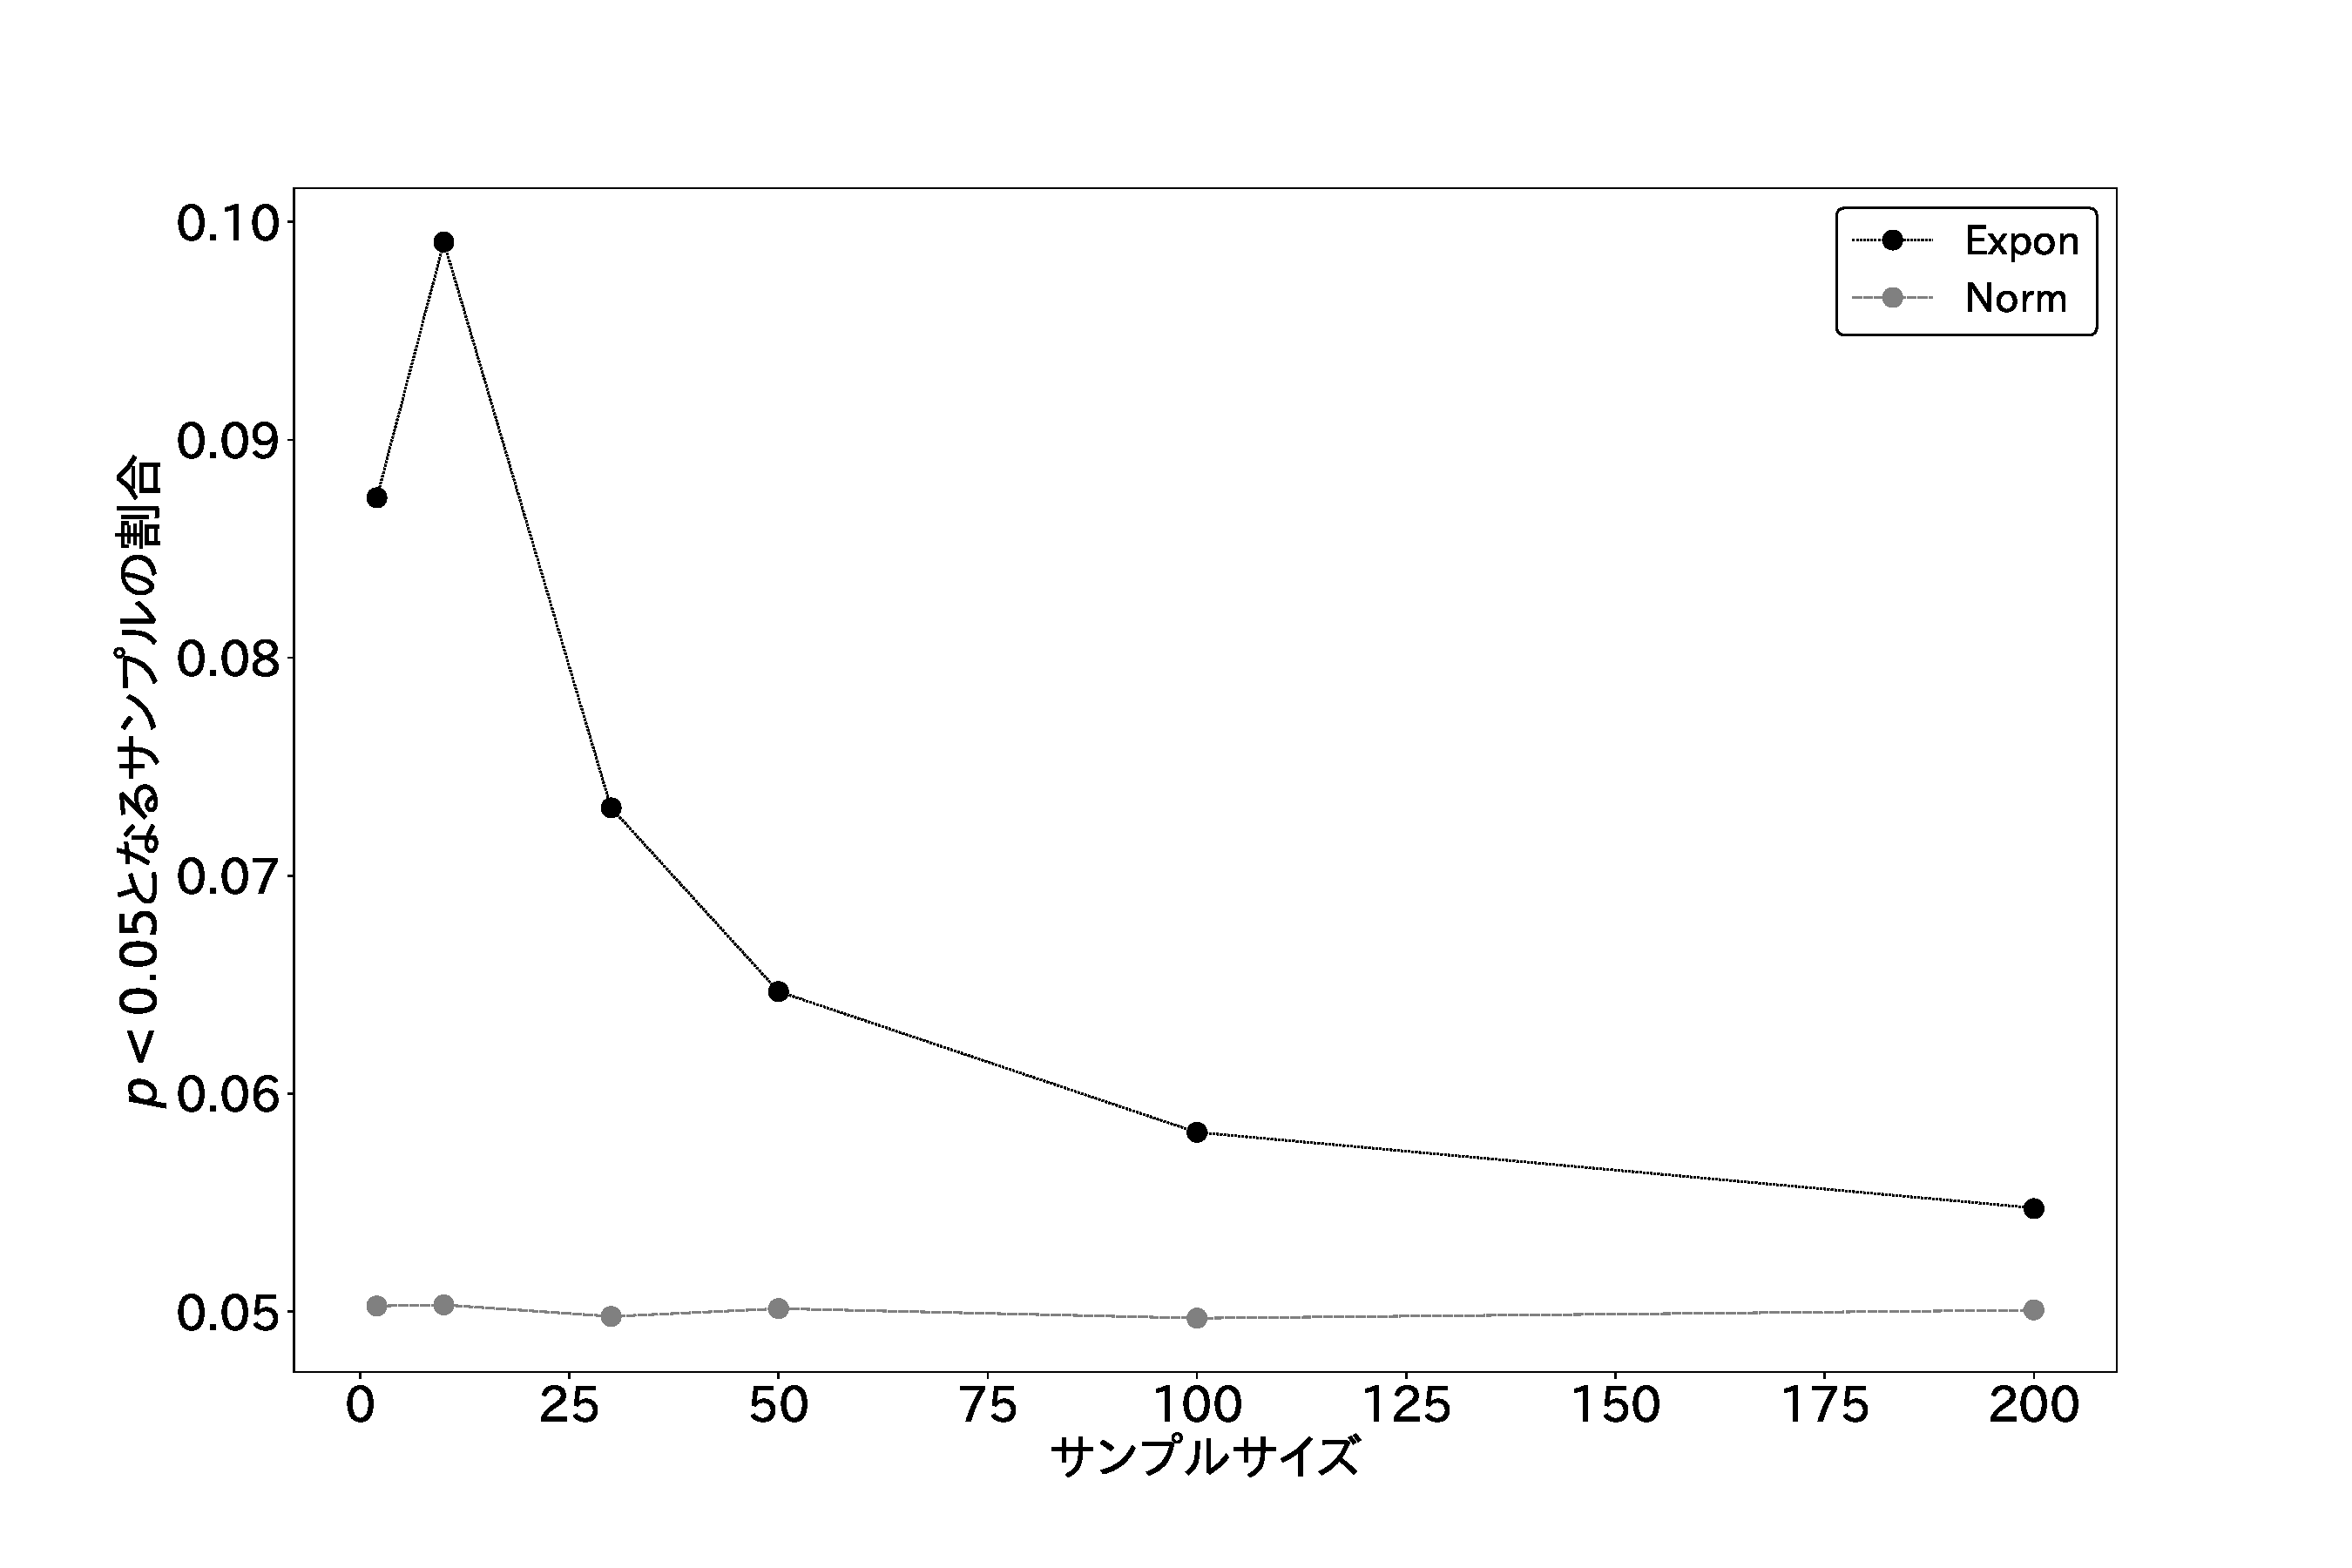
\includegraphics[width=15cm]{../markdown/section1/t_test_expon_norm.pdf}
        \caption{正規分布または指数ぶんぷから得た標本の$T$値から計算した$p$値で、$p<0.05$以下になる割合}
    \end{center}
\end{figure}

シミュレーションの結果、正規分布から標本を得た場合、$p<0.05$になる割合は、サンプルサイズに依存せず、$5\%$程度であり、期待通りである。
一方で、指数分布から標本を得た場合、$p<0.05$になる割合はサンプルサイズに応じて変化しており、また、どのサンプルサイズでも$p<0.05$となる割合は$5\%$より多い。

このことから、指数分布を含んだ統計モデルの$\alpha_1$は、$\alpha_1>0.05$であることがわかり、統計検定量を正しく選ばなかったことで、第一の過誤が期待した$0.05$よりも大きくなっていることがわかる。

\if 0
\subsubsection{いつでも正規分布を含んだ統計モデルでいこう}
データが非対称に分布しているのに、統計モデルに正規分布を指定した場合、推定が正しく行えないことを確認しておこう\footnote{元ネタ。
    小標本 t 検定の誤解:中心極限定理と一般化線形モデル 井口豊(生物科学研究所,長野県岡谷市)\url{https://biolab.sakura.ne.jp/small-sample-t-test-glm.html}}。
次のような統計モデルを構築する。
\begin{enumerate}
    \item $X_1,X_2,\cdots,X_n $はi.i.d
    \item 正規分布
    \item 正規分布の母数$\mu$,$\sigma^2$の値は不明
\end{enumerate}
正規分布の母数$\mu=1$とした統計モデルを$M(1)$と記述する。
この$X_1,X_2,\cdots,X_n$について次の統計量が$t(n)$分布に従うことがわかっている。
\begin{equation*}
    T = \frac{\bar{X}-1}{\sqrt{\frac{\sigma^2}{n}}} \sim t(n)
\end{equation*}
このとき、データが、既知の確率分布から得られた場合に、$p$値がサンプルサイズによってどのように変化するのかを調べる。
具体的に、平均$1$の指数分布または、平均$1$、標準偏差$1$の正規分布からサンプルを得て標本を作る。その標本を$100000$回取得する。
このとき、$T$値を計算し、$T$値いじょの値が得られる確率$p$を計算する。その$p$が$p<0.05$となる割合を計算する。以上をサンプルサイズを変化させてシミュレーションを行なった。

平均$1$、標準偏差$1$の正規分布の場合、統計モデルの仮定と一致するので、$T$値は$t(n)$分布に従う。よって、$p<0.05$となる頻度も、$5\%$程度になることが期待される。
一方で、平均$1$の指数分布の場合、統計モデルの仮定と一致しない。このことから、$T$は$t(n)$分布に従うとはいえない。このことから、$p<0.05$となる頻度はわからない。


\begin{figure}
    \begin{center}
        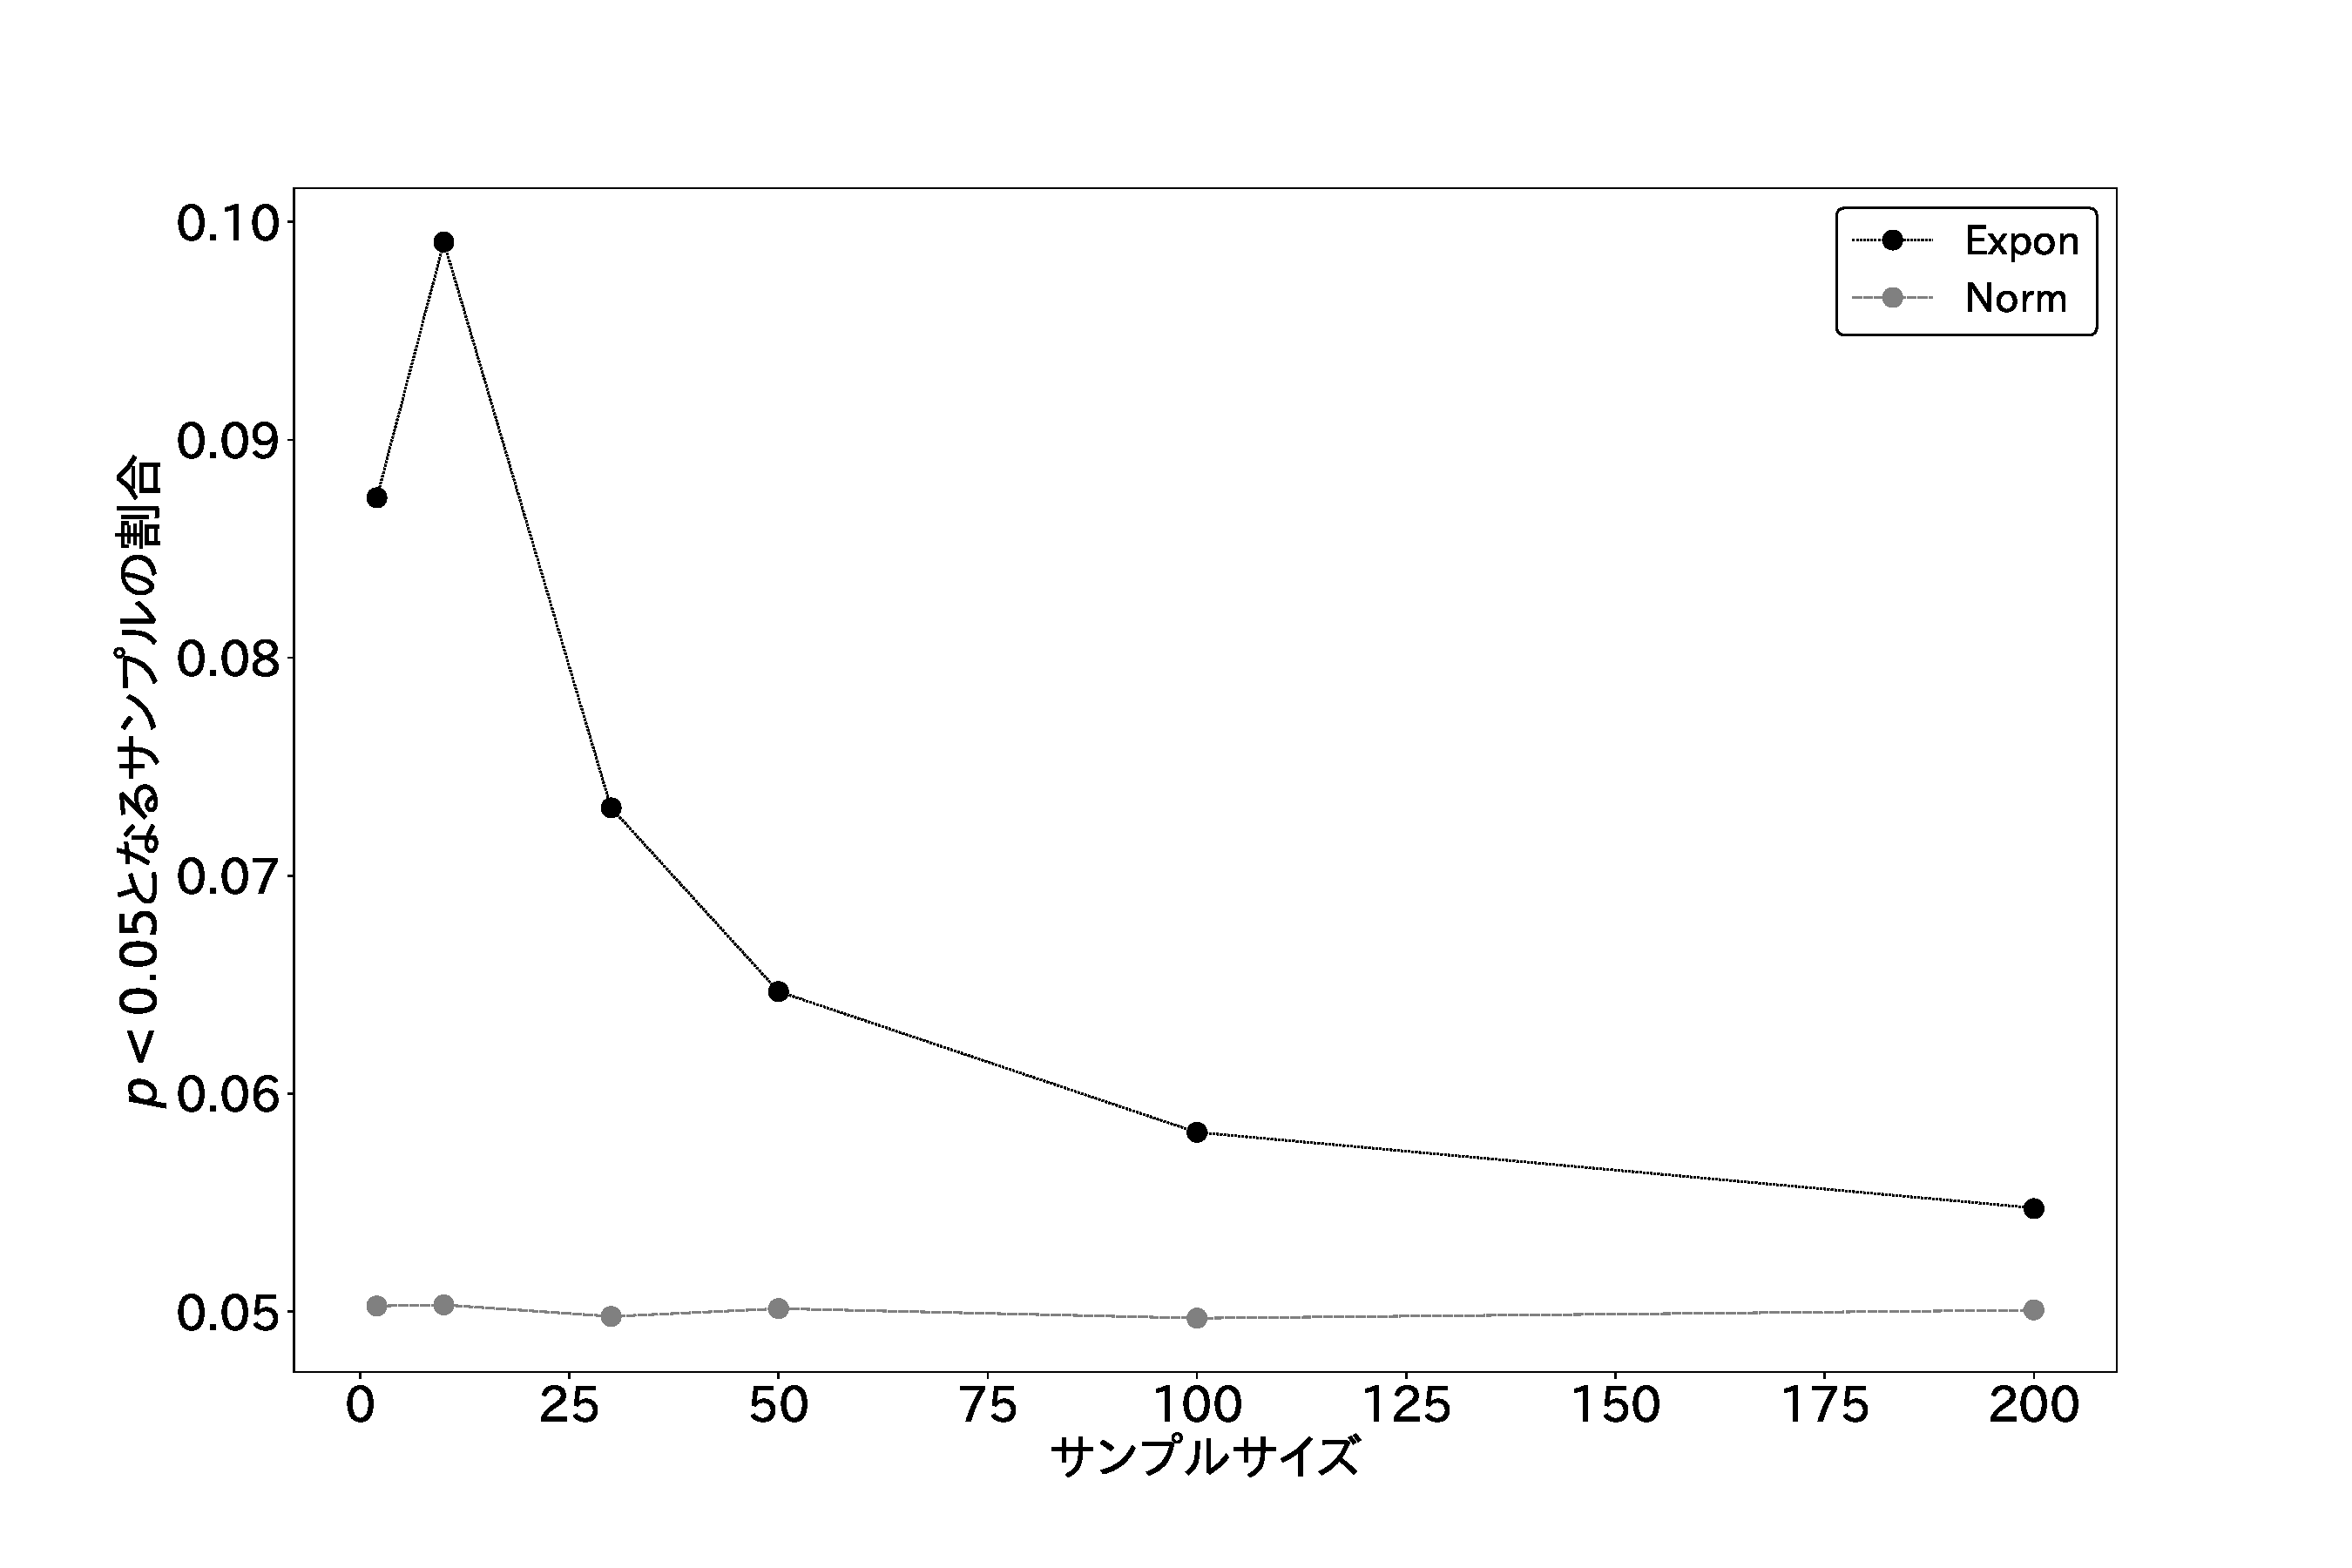
\includegraphics[width=15cm]{../markdown/section1/t_test_expon_norm.pdf}
        \caption{正規分布または指数ぶんぷから得た標本の$T$値から計算した$p$値で、$p<0.05$以下になる割合}
    \end{center}
\end{figure}

シミュレーションの結果、正規分布から標本を得た場合、$p<0.05$になる割合は、サンプルサイズに依存せず、$5\%$程度であり、理論と一致する。
一方で、指数分布から標本を得た場合、$p<0.05$になる割合はサンプルサイズに応じて変化しており、また、どのサンプルサイズでも$p<0.05$となる割合は$5\%$より多い。
このように、データが正規分布とかけ離れているにもかかわらず、正規分布を含んだ統計モデルを構築し、そこから統計量を計算しても、的外れになることがあることを示唆している\footnote{$n$を大きくしたとき、中心極限定理より、$p<0.05$となる割合も$5\%$に近づくと解釈することがある。本当だろうか。具体的には、次の定理が成り立つのだろうか。
\begin{quote}
\begin{theo}
    $X_1,X_2,\cdots,X_n \sim Exp(\lambda)$とするとき、$T=\frac{\bar{X}-1/\lambda}{\sqrt{\frac{S^2}{n}}}$ここで、$S^2=\frac{1}{n-1}\sum_{i=1}^n(X_i-\bar{X})^2$である。$T\sim t(n-1)$または、$t$がなんらかの統計分布に従う。または、$E[T]<\infty,Var[T]<\infty$
\end{theo}
\end{quote}
このことが成り立つなら、中心極限定理も成立し、$n$が十分大きいときに、分布関数を近似できそうである。
}
\fi
\begin{mybox}
    \begin{quote}
        \paragraph{サンプルサイズがxx以上あるから$t$検定}
        サンプルサイズがある値以上あるので、中心極限定理により、$t$検定が利用できるというものもある\footnote{http://id.ndl.go.jp/bib/024660739}。このロジックが読み込めなかったので、その謎を明らかにすべく我々はアマゾンの奥地へ向かった。

        確かに、サンプルサイズが1以上であれば、$t$検定を行うことは原理的には可能である。
        一方で、データが指数分布的であるときに、$t$検定を使うときに生じる問題は上でみた通りであり、$p<0.05$となる標本の割合が多くなっているので、間違った推測をする可能性が高くなる。
        他の分布関数でもおそらく同じような現象が現れる。
        このことから、我々は「$t$検定が利用可能である」は正確ではなく、「$t$検定を使うことができるが、間違った推測である確率が高くなる」ということだと推察した。
    \end{quote}
\end{mybox}

\subsubsection{検定を繰り返し使おう($\alpha_2$)}
次の統計モデルによって複数の標本について推測することを考える。
\begin{enumerate}
    \item $X_1,X_2,\cdots,X_n $はi.i.d
    \item 正規分布
    \item $\mu$,$\sigma^2=10$
\end{enumerate}
ここまでは、一つの標本に対して、統計モデル$M(\mu)$により推測できるかを考えていた。
ここでは、複数の標本について、$M(\mu)$により推測できるかを統計検定を指標にし考える。
標本が$3$個あるとする。このとき、それぞれの標本の統計検定量$T$が信頼区間に入っている確率は、$(1-\alpha)$である。全ての標本の統計検定量$T$が信頼区間に入っている確率は、その積$(1-\alpha)\times(1-\alpha)\times(1-\alpha)=(1-\alpha)^3$であり、この確率で統計モデルは棄却されない。
一方で、棄却される確率は、$1-(1-\alpha)^3$である。
\begin{table}[hbtp]
    \caption{標本数に応じた$\alpha_2$}
    \label{table:multiple_test_reject_prob}
    \centering
    \begin{tabular}{lcr}
      \hline
      標本数  & $\alpha=0.05$  &  $\alpha=0.01$ \\
      \hline \hline
       1 & $0.05$  & $0.01$ \\
       2 & $0.0975$ & $0.0199$\\
       3 & $0.142$ & $0.0297$\\
       4 & $0.185$ & $0.0394$\\
    \end{tabular}
  \end{table}
表\ref{table:multiple_test_reject_prob}は、標本数に応じた$\alpha_2$である。標本数が大きくなるについれて、$\alpha_2$が大きくなることがわかる。

$\alpha_1$がレベル$\alpha$の検定になっていない場合、$\alpha_2$はさらに有意水準$\alpha$から隔たりの多い数値になる。




\subsection{第二の過誤}
統計モデルの間の類似度を検出力といった。この検出力は、統計モデルに対して、適切な統計量を与えられたときに計算が可能であるが、不適切な統計量を与えたとき、検出力を歪めてしまうことがある。これを第二の過誤(type II error)といい、その確率を$\beta'$で表す。

\subsection{標準偏差か標準誤差か}
標準偏差や標準誤差によりデータのばらつきを捉えようとすることは、正規分布を含んだモデルを使って、母集団を推測しようとする行為であると考えることができます。以下の議論は、モデルが現象をよく捉えている場合にはうまく成り立つが、そうでないなら、モデルを修正したほうが、うまく現象をうまく捉えることができる\footnote{様々な意見がある\cite{SUZUKI_SESD,池田郁男2013統計検定を理解せずに使っている人のために,池田郁男2019改訂増補版}}。
ここでは、次のモデル$M(\mu,\sigma^2)$を使う。

\begin{enumerate}
    \item i.i.d
    \item 正規分布関数
    \item $\mu,\sigma^2$
\end{enumerate}
ここで、母集団から無作為抽出した標本の標本平均と標本分散をそれぞれ、$\bar{x}=\frac{1}{n}\sum{x_i},s^2=\frac{1}{n}\sum(x_i-\bar{x})^2$である。これらを組み入れた統計モデルを$M(\bar{X},s^2)$と書く。

\subsubsection{標準偏差}
正規分布を含んだ統計モデルを仮定し、そのモデルの上で、予想されるサンプルがおよそ$68\%$の確率で出現する範囲は、母数分散$\sigma^2$より以下の範囲になります。
\begin{equation*}
    [\mu-\sigma,\mu+\sigma].
\end{equation*}
モデルの母数分散は不明な場合、母集団から無作為抽出を行なって集計した標本の偏差$s$を計算します。
\begin{equation*}
    s = \sqrt{\frac{1}{n}\sum(x_i-\bar{x})^2}.
\end{equation*}
このことから、モデルが予測するサンプルが$68\%$の確率で出現する範囲は
\begin{equation*}
    [\mu-s,\mu+s].
\end{equation*}
これを図示したものが、図です。
言い換えれば、これは、$68\%$予測区間である。


\begin{figure}
    \begin{center}
        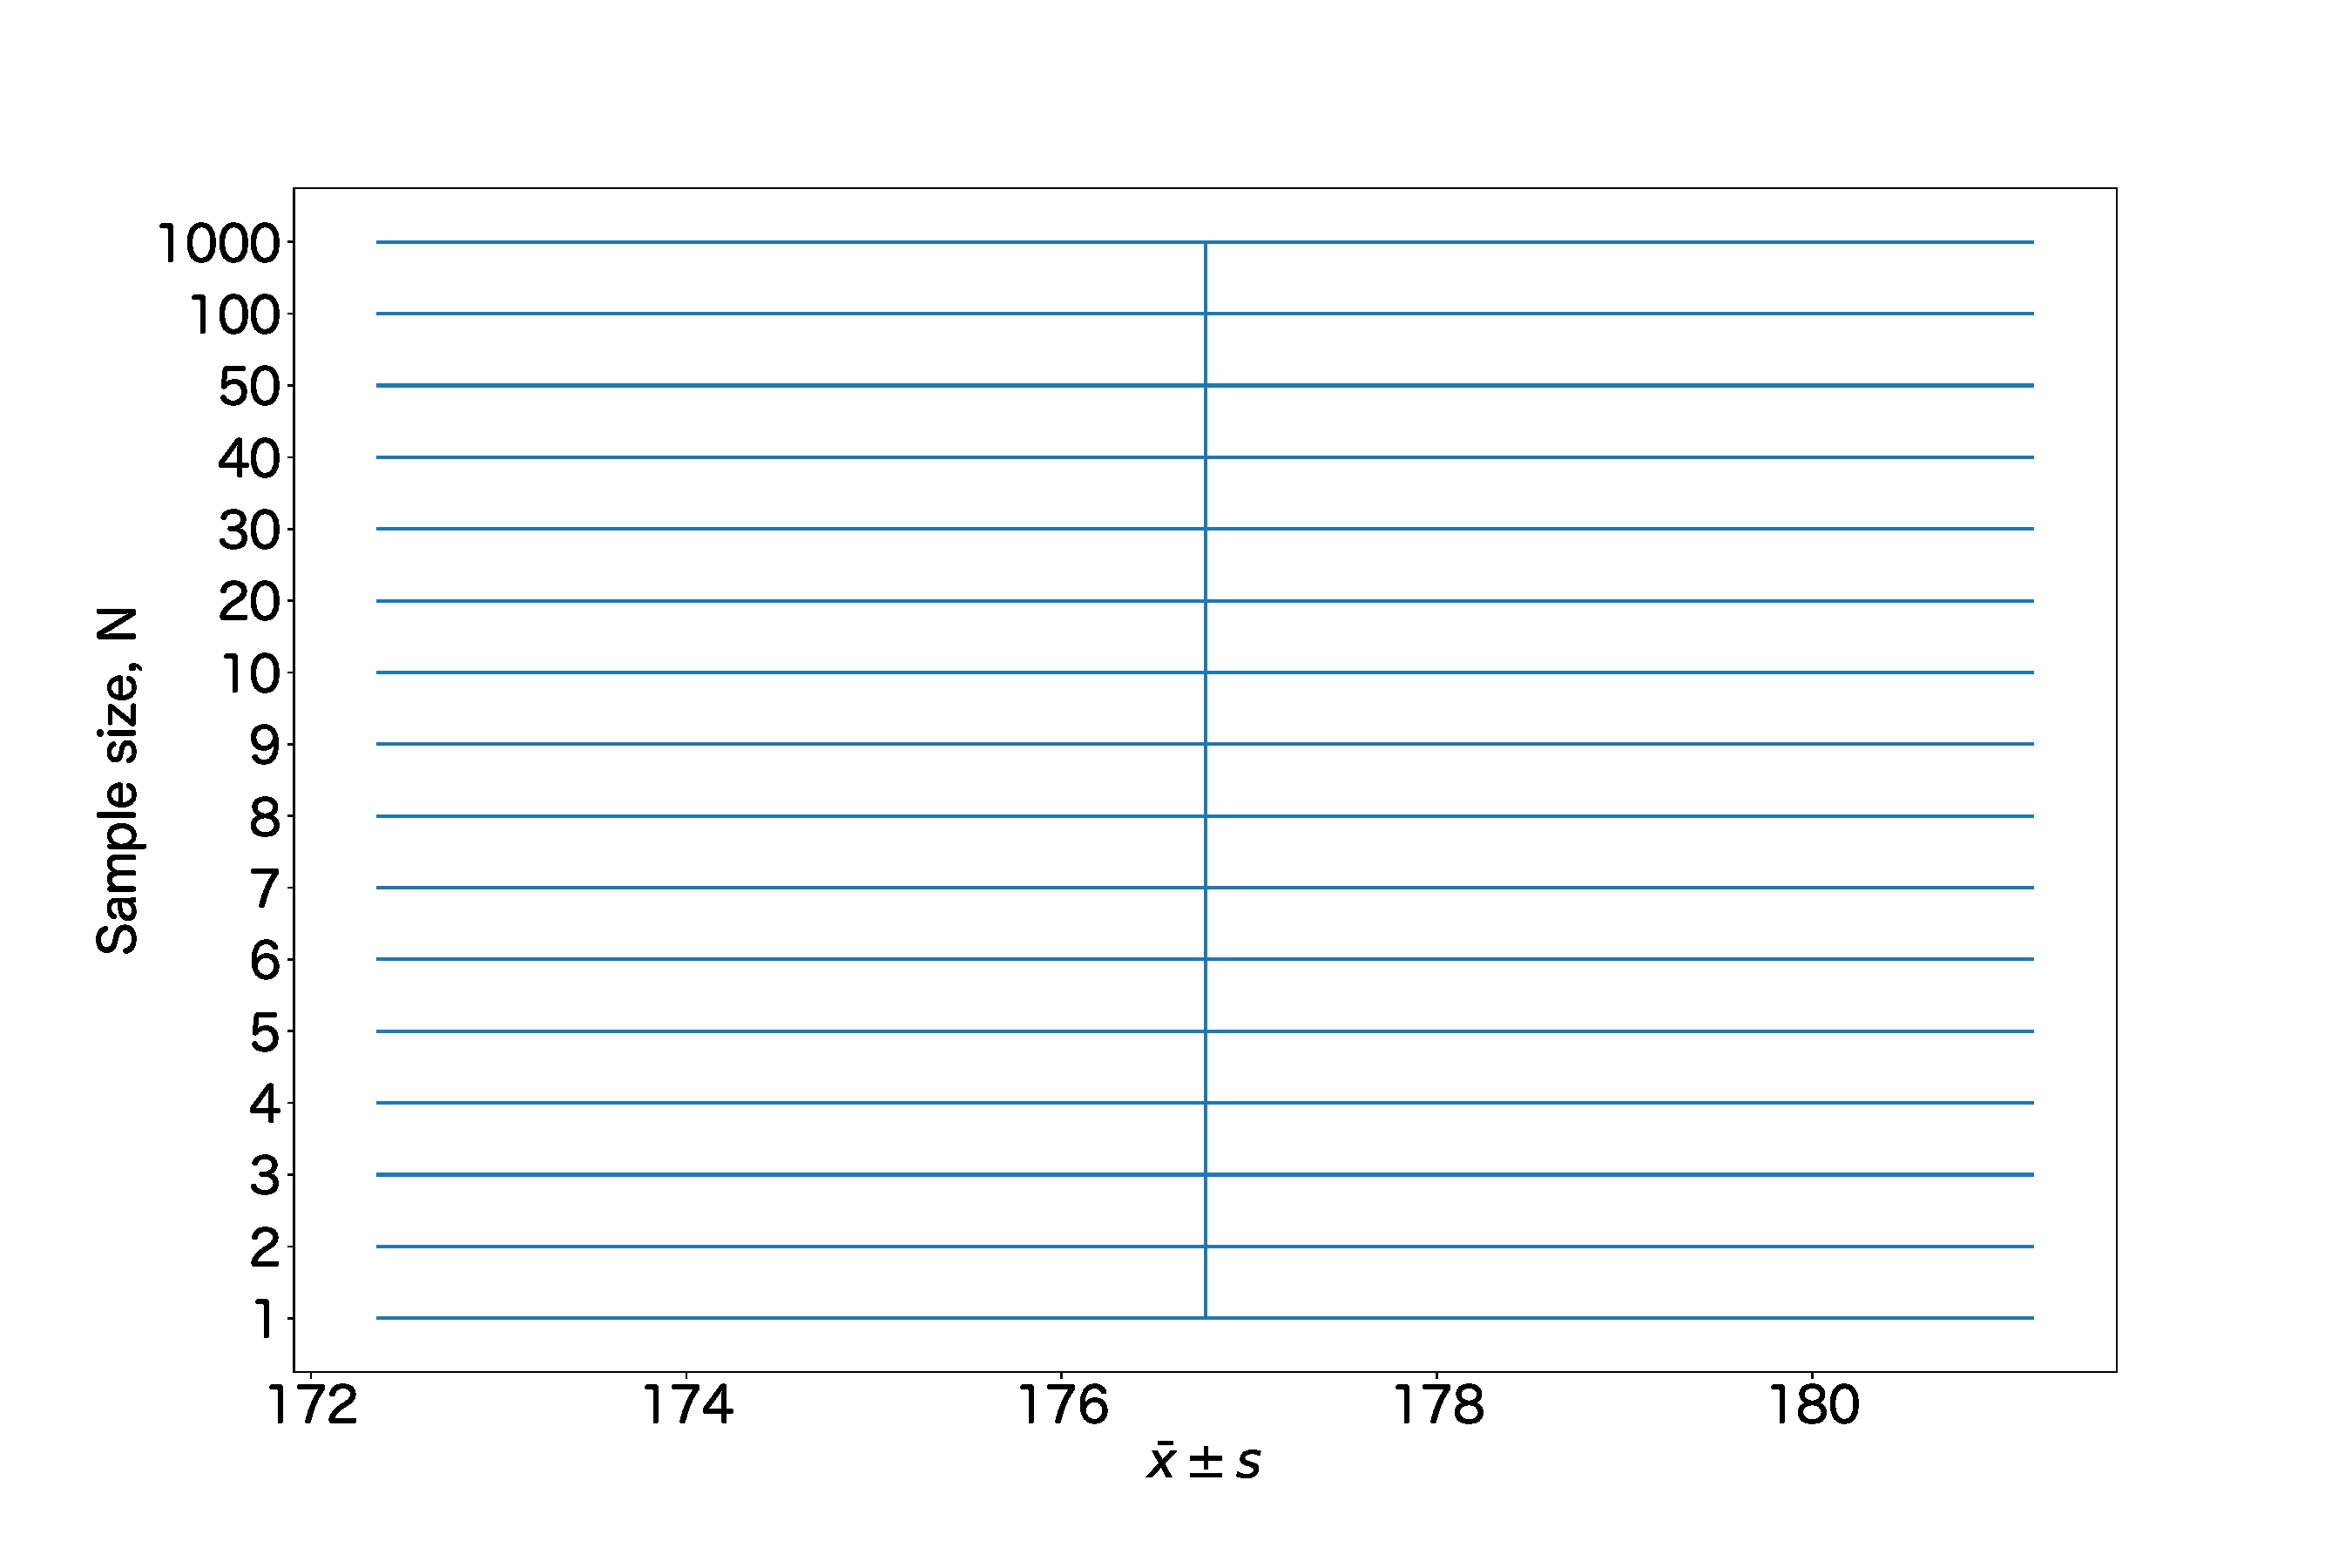
\includegraphics[width=15cm]{../markdown/section1/Norm_standard_deviation.pdf}
        \caption{サンプルサイズに応じた標準誤差の広がり}
        %\label{fig:standard_normal_distribution}
    \end{center}
\end{figure}



\subsubsection{標準誤差}
標準誤差$SE$は、標準偏差$s$をサンプルサイズ$N$の平方根で割ったものである。
\begin{equation*}
    SE = \frac{s}{\sqrt{N}}
\end{equation*}
$\bar{x}\sim N(\mu,\sigma^2/\sqrt(N))$であるので、モデルの上で$\bar{x}$が以下の範囲に出現する確率は、およそ$68.2\%$である。
\begin{equation*}
    [\bar{\mu}-SE,\bar{\mu}+SE]
\end{equation*}
よって、$\mu$の値は一般にわからないので、標本平均$\bar{X}$を用いて、
\begin{equation*}
    [\bar{X}-SE,\bar{X}+SE]
\end{equation*}
である。
統計モデル$M(\bar{x},s^2)$からサンプリングした$\bar{X}$がこの範囲に得られる確率が$68.2\%$である\footnote{$\sigma$が変曲点であるから使ったと思われるが、なぜ、$68.2\%$または、$\bar{X}\pm SE$の範囲を使ったのかはわからなかった。誤差論の教科書なども調べてみる必要があると思う。}
\footnote{標準偏差に ± を付けるな!: 医療論文に多い?
\url{https://biolab.sakura.ne.jp/mean-sd.html}。まだ読めていない。$\pm SE$という表記はよろしくないらしい。}。
言い換えれば、$SE$は、$68\%$信頼区間である。


\begin{figure}
    \begin{center}
        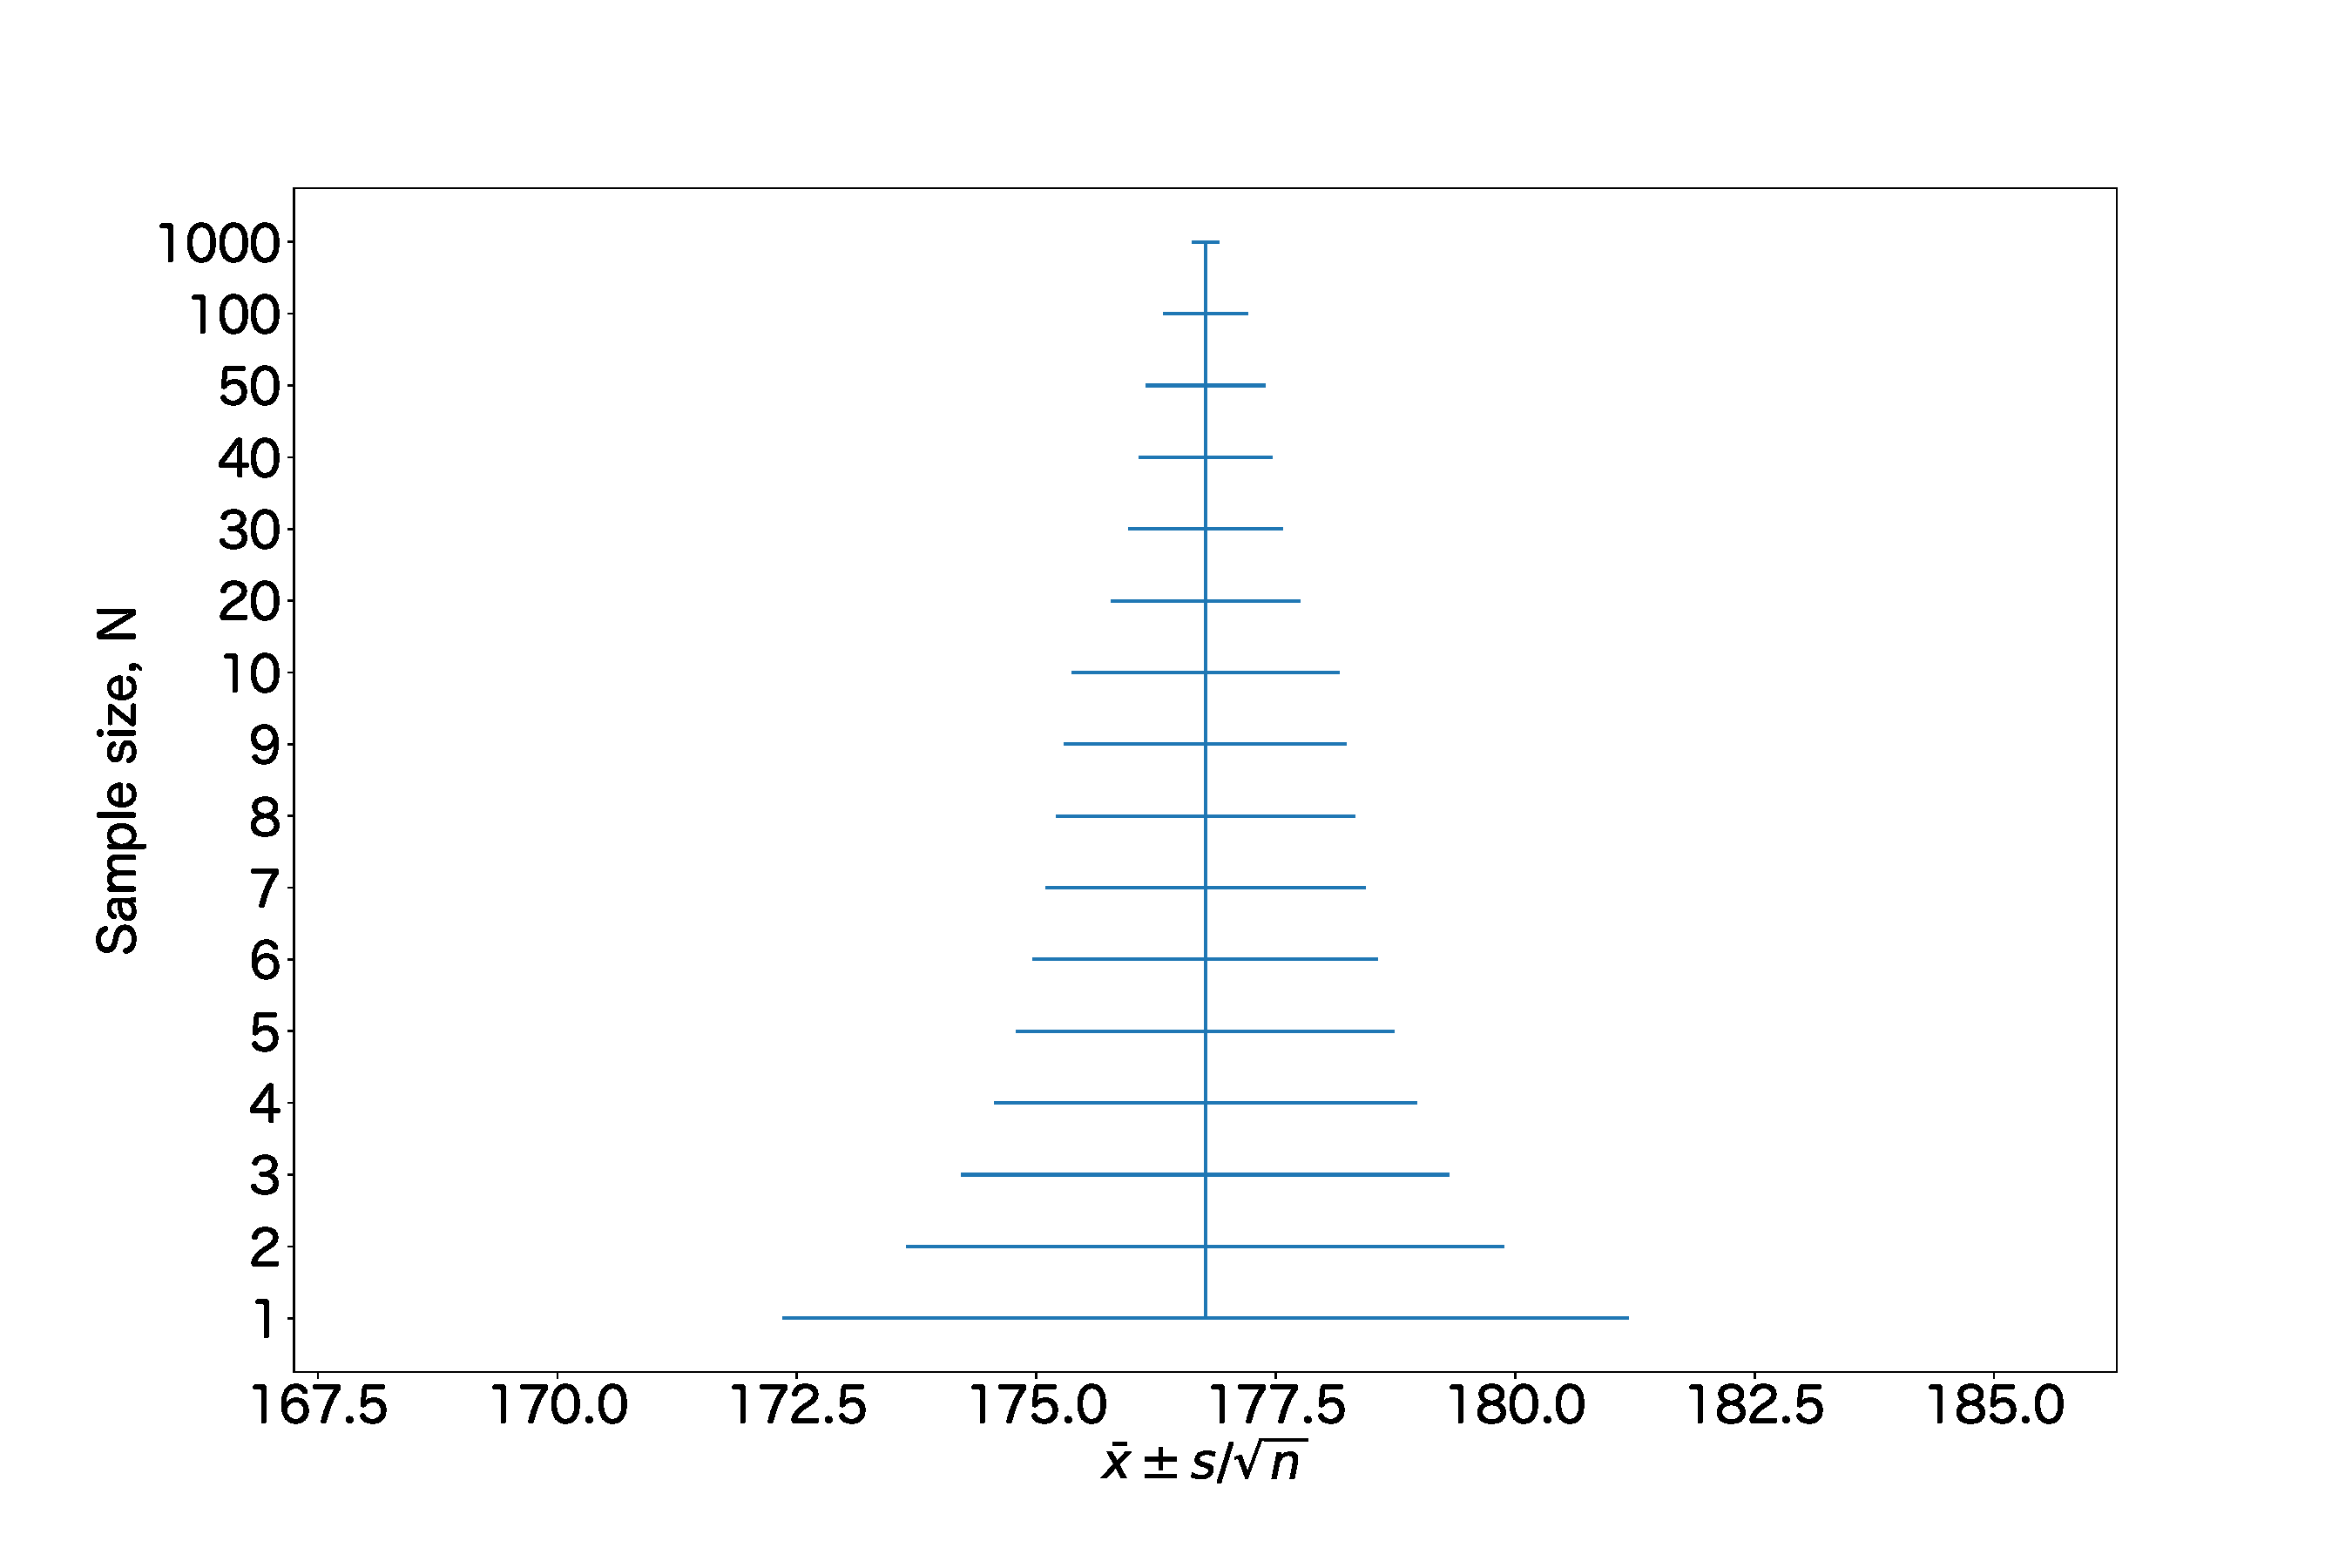
\includegraphics[width=15cm]{../markdown/section1/Norm_SE.pdf}
        \caption{サンプルサイズに応じた標準偏差の広がり}
        %\label{fig:standard_normal_distribution}
    \end{center}
\end{figure}
    
\subsubsection{母集団の標本が指数分布的に分布していた場合}
母集団の分布形と統計モデルに含まれている確率分布関数が著しく異なる場合を考える。
母集団分布の分布として、指数分布を仮定し、そこから無作為抽出によりサンプルサイズ$10^6$の標本を得たとする。
標準偏差の間にサンプルが含まれる確率を計算する。この結果、期待していた値よりも著しく大きな確率$86\%$程度を得る。

\begin{lstlisting}
N = 10**6
sample = expon.rvs(scale=10,size=N)
#sample = norm.rvs(loc=0,scale=1,size=N)
lambd= np.average(sample)
print(np.average(sample),np.std(sample),np.var(sample))

mu = np.average(sample)
s = np.std(sample)

a,b = mu-s,mu+s
len(sample[np.where( (sample >a) & (sample<b) )])/N
\end{lstlisting}

以上でわかるのは、統計モデルと実際の母集団が乖離している場合には、標準誤差に間違いが多くなるということである。


\section{モデルと標本の乖離による過誤}
データとモデルを統計検定量により比較したとき、その乖離について測ることのできないことをまとめる。

\subsection{モデルの確率密度関数と標本の分布の乖離による過誤}
経験がないことで、適当なモデルを構築し、非常に少数のサンプルサイズしか得られないことで、そのモデルの妥当性について検証できないまま、モデルとデータを統計検定により比較し、判断することにより生じる間違いである。
例えば、データの分布が非対称に分布しているのに、正規分布を含んだ統計モデルを構築し、$T$統計量により検定をおこなったとする\footnote{データが非対称に分布していることから、正規分布を含んだ統計モデルでは推論できないことがわかるので、統計検定を使う意義はなくなると思う}。前の節でみたように、分布関数に対して適切な統計量を選ばなければ$\alpha_1$が設定した有意水準$\alpha$とならないので、期待していた推論が行えないことが多くなる。

\subsection{無作為抽出されていない事による過誤}
対象を無作為に抽出できていない場合、その推定は誤差が大きくなり、誤りが多くなる。
例えば、17歳の日本人男性の身長を母集団に指定したのに、17歳のバスケ部部員の身長を計測すると、その標本はひどく偏ったものになる。その標本を元に、モデルの母数を推定し、母集団に関する推測を行うと、間違った推測が得られる。例えば、平均が大きくなりすぎたりすることが予想される。


\subsubsection{後付けの母集団かつ$p<\alpha$を満たす集団}
$p<\alpha$であるという標本がデータから発見されたので、標本の特性を持つと思われる母集団を後付けし、その母集団から無作為抽出を行なったことにし、統計モデルが棄却されたというストーリーを作ったとする。
言い換えれば、後付けの母集団ならば、$p<\alpha$であるという論理を構築したことになる。
実際には、後付けの母集団でありかつ$p<\alpha$という集団から作為抽出しているので\footnote{この場合でも無作為抽出できていると誤解してしまうが、後付けの母集団から無作為抽出できていない!}、本来の母集団については何もわからない。言い換えれば、母集団に関する拡大解釈が行われたことで、母集団に関しては何もわからないのに、推測を行なったと間違えた主張をしている\footnote{母集団デカすぎの過誤である}。
母集団の特徴を知るには、無作為抽出を行い、推測を行う必要がある。

このような母集団に関する拡大解釈を仮説ハッキング($HARKing$)といい、この操作により得たデータと仮説について、仮説が元からあったことにして、報告を行うと、研究不正となる\footnote{
    HARKingは、再現性の問題という意見もある。
    \url{https://twitter.com/ykamit/status/1077716200845500416}。この意見に私は同意する。私は、母集団を無作為抽出していないことで、再現できないことが増えると考えている。
}
\footnote{
    多重検定により、$p$値が低く推測されることが問題であるというものもある\cite{池田_功毅2016,中村_大輝2021sp20016}。部分的には同意できるが、私は十分理解できなかった。
}\footnote{
    Twitterでのアンケートでは、多くの人がHARkingをうまく理解できてないという調査もある。
    \url{https://twitter.com/biomedcircus/status/1088957697368690689}
}\footnote{
    探索的なデータ解析においては、帰無仮説の後付けが許されるという主張もある。この意見には同意できない。母集団について拡大解釈をすることは許されない。探索的データ解析により得られるのは、母集団かつ$p<\alpha$という集団が見つかったということのみ主張でき、母集団についての推測をしたと主張してはいけない。
}\footnote{
    HARKingについては、\cite{kerr1998harking}に詳しくまとめられている
}。


\subsubsection{$p<\alpha$になったら無作為抽出を終える}
$p$値がある値を下回ったときに、実験を終了するという操作を行なった場合も、無作為抽出したとは言い難い。
この不正な操作をアステリスクシーキングという。




\if 0
\paragraph{$p<0.05$にした理由}
https://biolab.sakura.ne.jp/statistics-5-percent.html
\fi



\if 0
\subsection{サンプルサイズが小さければ$t$検定}
西内啓 著「統計学が最強の学問である(実践編)」(ダイヤモンド社)
\url{https://biolab.sakura.ne.jp/small-sample-t-test-glm.html}
\fi 

\section{指数分布を使った統計モデル}
あるシステムの故障発生間隔日数を調べてみると、次のようなデータを得たとする(実際には、平均10の指数分布関数を使いサンプリングを行った。もちろんそんなことは忘れて、現象は数学関数により生成されていないと考える)
\begin{lstlisting}
19.9290003   0.60892905  0.55864947 29.77846887  0.28955969  1.58223429 21.10080586 10.78952122  0.59624638 15.74379646
\end{lstlisting}


平均値は10.09,分散は107.7であった。以下の仮定からなる統計モデルを構築した。
\begin{quote}
    \begin{enumerate}[(1)]
\item i.i.d
\item 正規分布
\item 平均10.09、分散107.7
\end{enumerate}
\end{quote}
では統計検定量を元に、$p$値を求めてみる。具体的には、

\begin{lstlisting}
Y =[19.9290003 ,  0.60892905,  0.55864947, 29.77846887,  0.28955969,  1.58223429, 21.10080586, 10.78952122,  0.59624638, 15.74379646]
stats.ttest_1samp(Y, 10.09)
\end{lstlisting}

結果、$p=0.978$である。$p=0.05$を基準にすれば、この統計モデルは棄却できない。統計モデルの仮定が妥当かを一つずつ調べる。統計モデルの仮定(2)は、分布が正規分布であることを仮定している。実際の標本をQ-Qプロットしてみよう。正規分布だと考えても問題がなさそうである。統計モデルの仮定(3)について検討する。このサンプルの平均値は$10.09$なので、これについても仮定は妥当だと考えられる。
では、帰無仮説を採択し、この統計モデルを元に推測をするべきだろうか。このモデルで推測を行なってみる。$15$日後の故障発生率は$P(X>20)=0.0036$程度である。同様に、$5$日後の故障発生率は、$P(X>5)=0.0036$である。正規分布は左右対称な関数なので、平均故障発生日から5日でも15日でも、同じ割合で故障する。 
機械などの故障は日数がたてば故障しやすくなるので、肌感覚としてあり得ないと思われる。
実際に、この統計モデルによる故障発生間隔の推測は現実と乖離していくことがわかっている。
このように、恣意的に決めた$p$より大きな統計モデルを使ったとしても、推測がうまくいくわけではないことから、棄却されなかった統計モデルを採用することには慎重になるべきである。

二つ目は、データの偏りによって、統計モデルを棄却できないことあるということである。
$10000$回実験を繰り返したとして(もちろん、指数分ぷからサンプリングを行った。もちろんそんなことは忘れて、現象は数学関数により生成されていないと考えてください)、サンプルサイズは毎回10だとすると、棄却できる割合は0程度であった。一方で、サンプルサイズを$100$程度にすると、棄却できる割合は、$0.956$程度であった。これは、平均値のあたりにデータが集まりやすく、データの端は無視できる程度の数量しか発生しないことで、正規分布を使った統計モデルを棄却しにくくなる。TODO
このように、データが十分ない場合は$p$の棄却に正規分布を仮定した統計モデルでは統計モデルを棄却する頻度は高くなることが予想される。

$p$値による判断がうまくいかないことがわかった。また、信頼区間の中にある母数でも推論ができないこともわかった。
\if 0
このような偏ったデータを手に入れた場合はどのように統計モデルを作ればいいのだろうか。
\fi

https://biolab.sakura.ne.jp/small-sample-t-test-glm.html



\subsubsection{モデルの更新}
\if 0
データ数の問題と、推測の精度の問題を解決することはできるだろうか?
尤度ひ検定
\fi
月日は流れ、データが蓄積された。その結果、次のような分布が得られた。ここまでの議論で、正規分布を仮定したモデルを棄却できないことはわかった。では、そのモデルを使って現在のデータを予測できるだろうか?パラメータを推定した正規分布とデータの分布を見てみよう。
データの最頻値が0の近くなので、平均10の正規分布では、ズレが生じることがわかる。
これではデータを捉えることはできない。
また、$30$日後までに故障が発生する確率を計算してみると、$0.971$程度であり、30よりも大きなデータの数は$0.05(1-0.05=0.95)$それなりに良く一致している。
一方で,5日までの故障発生率は、$0.30$をと予測するが、実際のデータは、0.18程度であり、こちらは乖離していると感じるだろう。
\begin{figure}
\begin{center}
    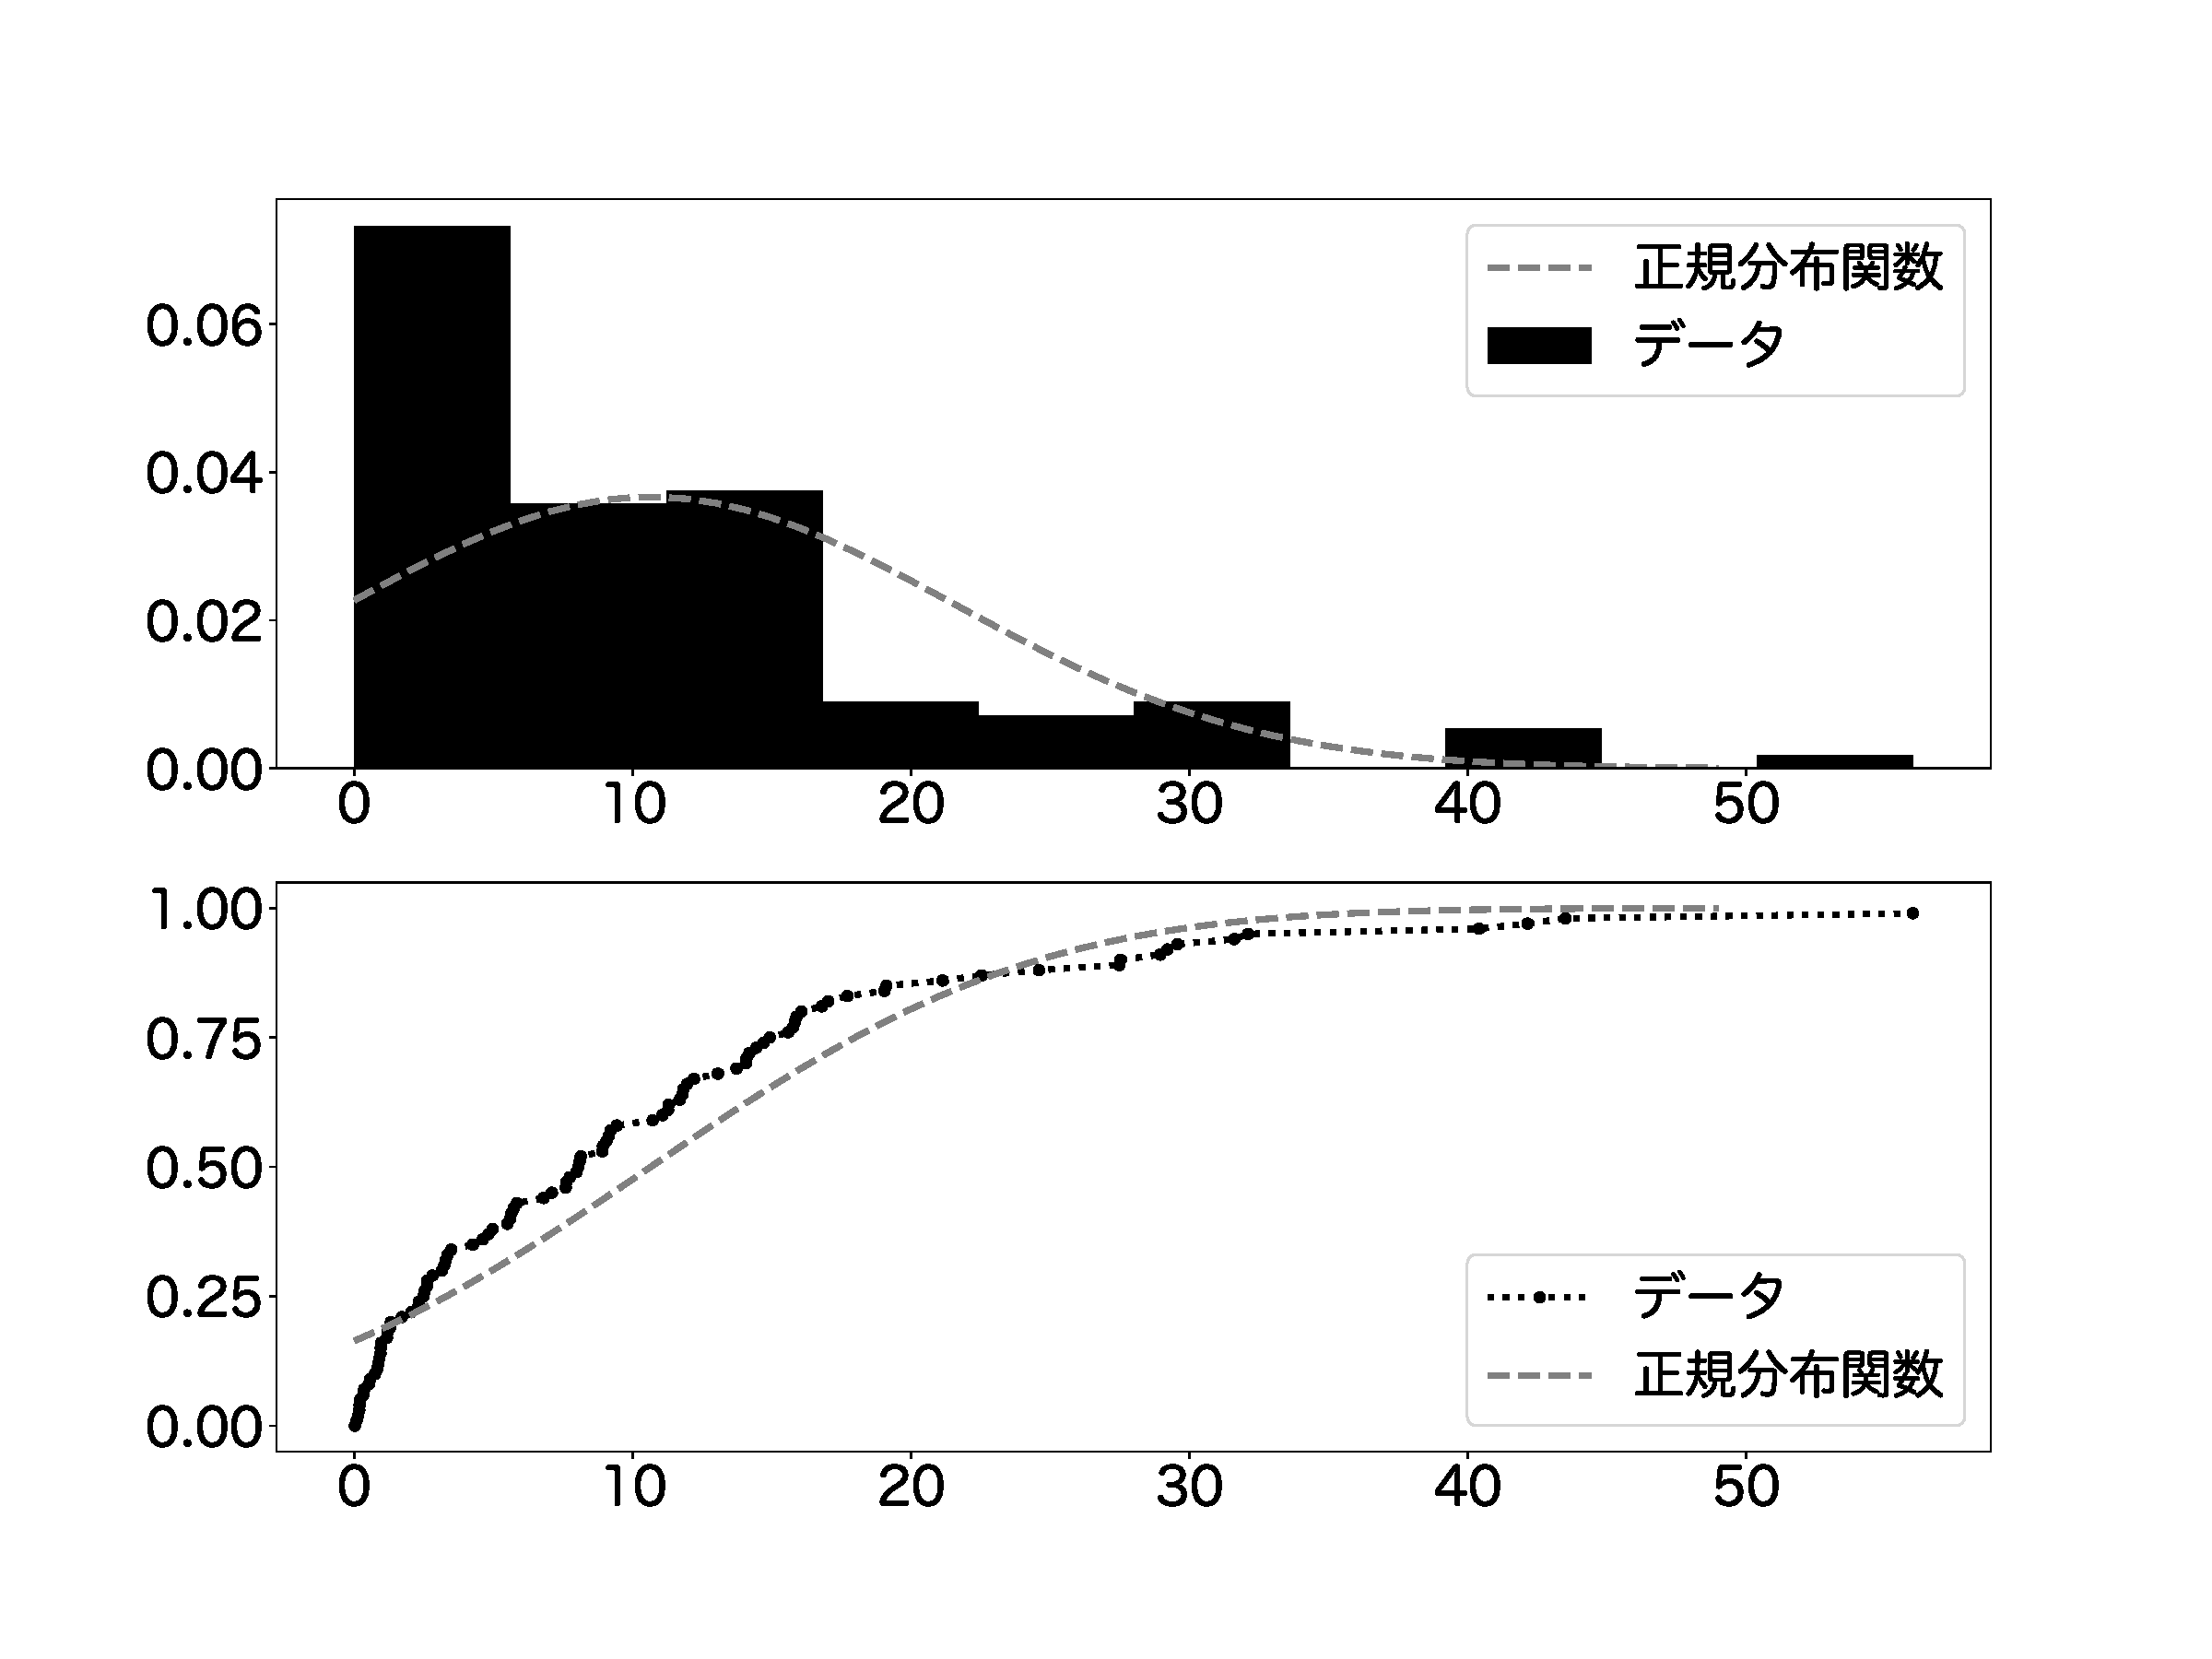
\includegraphics[width=15cm]{../markdown/section1/normal_exponential.pdf}
    %\caption{データの分布を正規分布で捉えれない}
\end{center}
\end{figure}


では、どのようなモデルを構築すればいいのだろうか。指数分布関数を使ってみよう
\begin{quote}
    \begin{enumerate}[(1)]
\item i.i.d
\item 指数分布
\item 母数$\lambda$
\end{enumerate}
\end{quote}
このモデルを$M(\lambda)$とかく。指数分布では、確率変数の平均は、母数$\lambda$の逆数であることがわかっている($E[x]=\frac{1}{\lambda}$)。$\lambda$として、現在手に入れたデータの平均値の逆数を代入し、データの分布と指数関数の曲線を書いてみると、よく一致しているように見える。

30日後に故障が起こる可能性は、$0.94$程度であると予想が出る。現状のデータと確認をしてみると、30よりも大きなデータの数は$0.05(1-0.05=0.95)$より、良く一致していることもわかる。
\begin{figure}
\begin{center}
    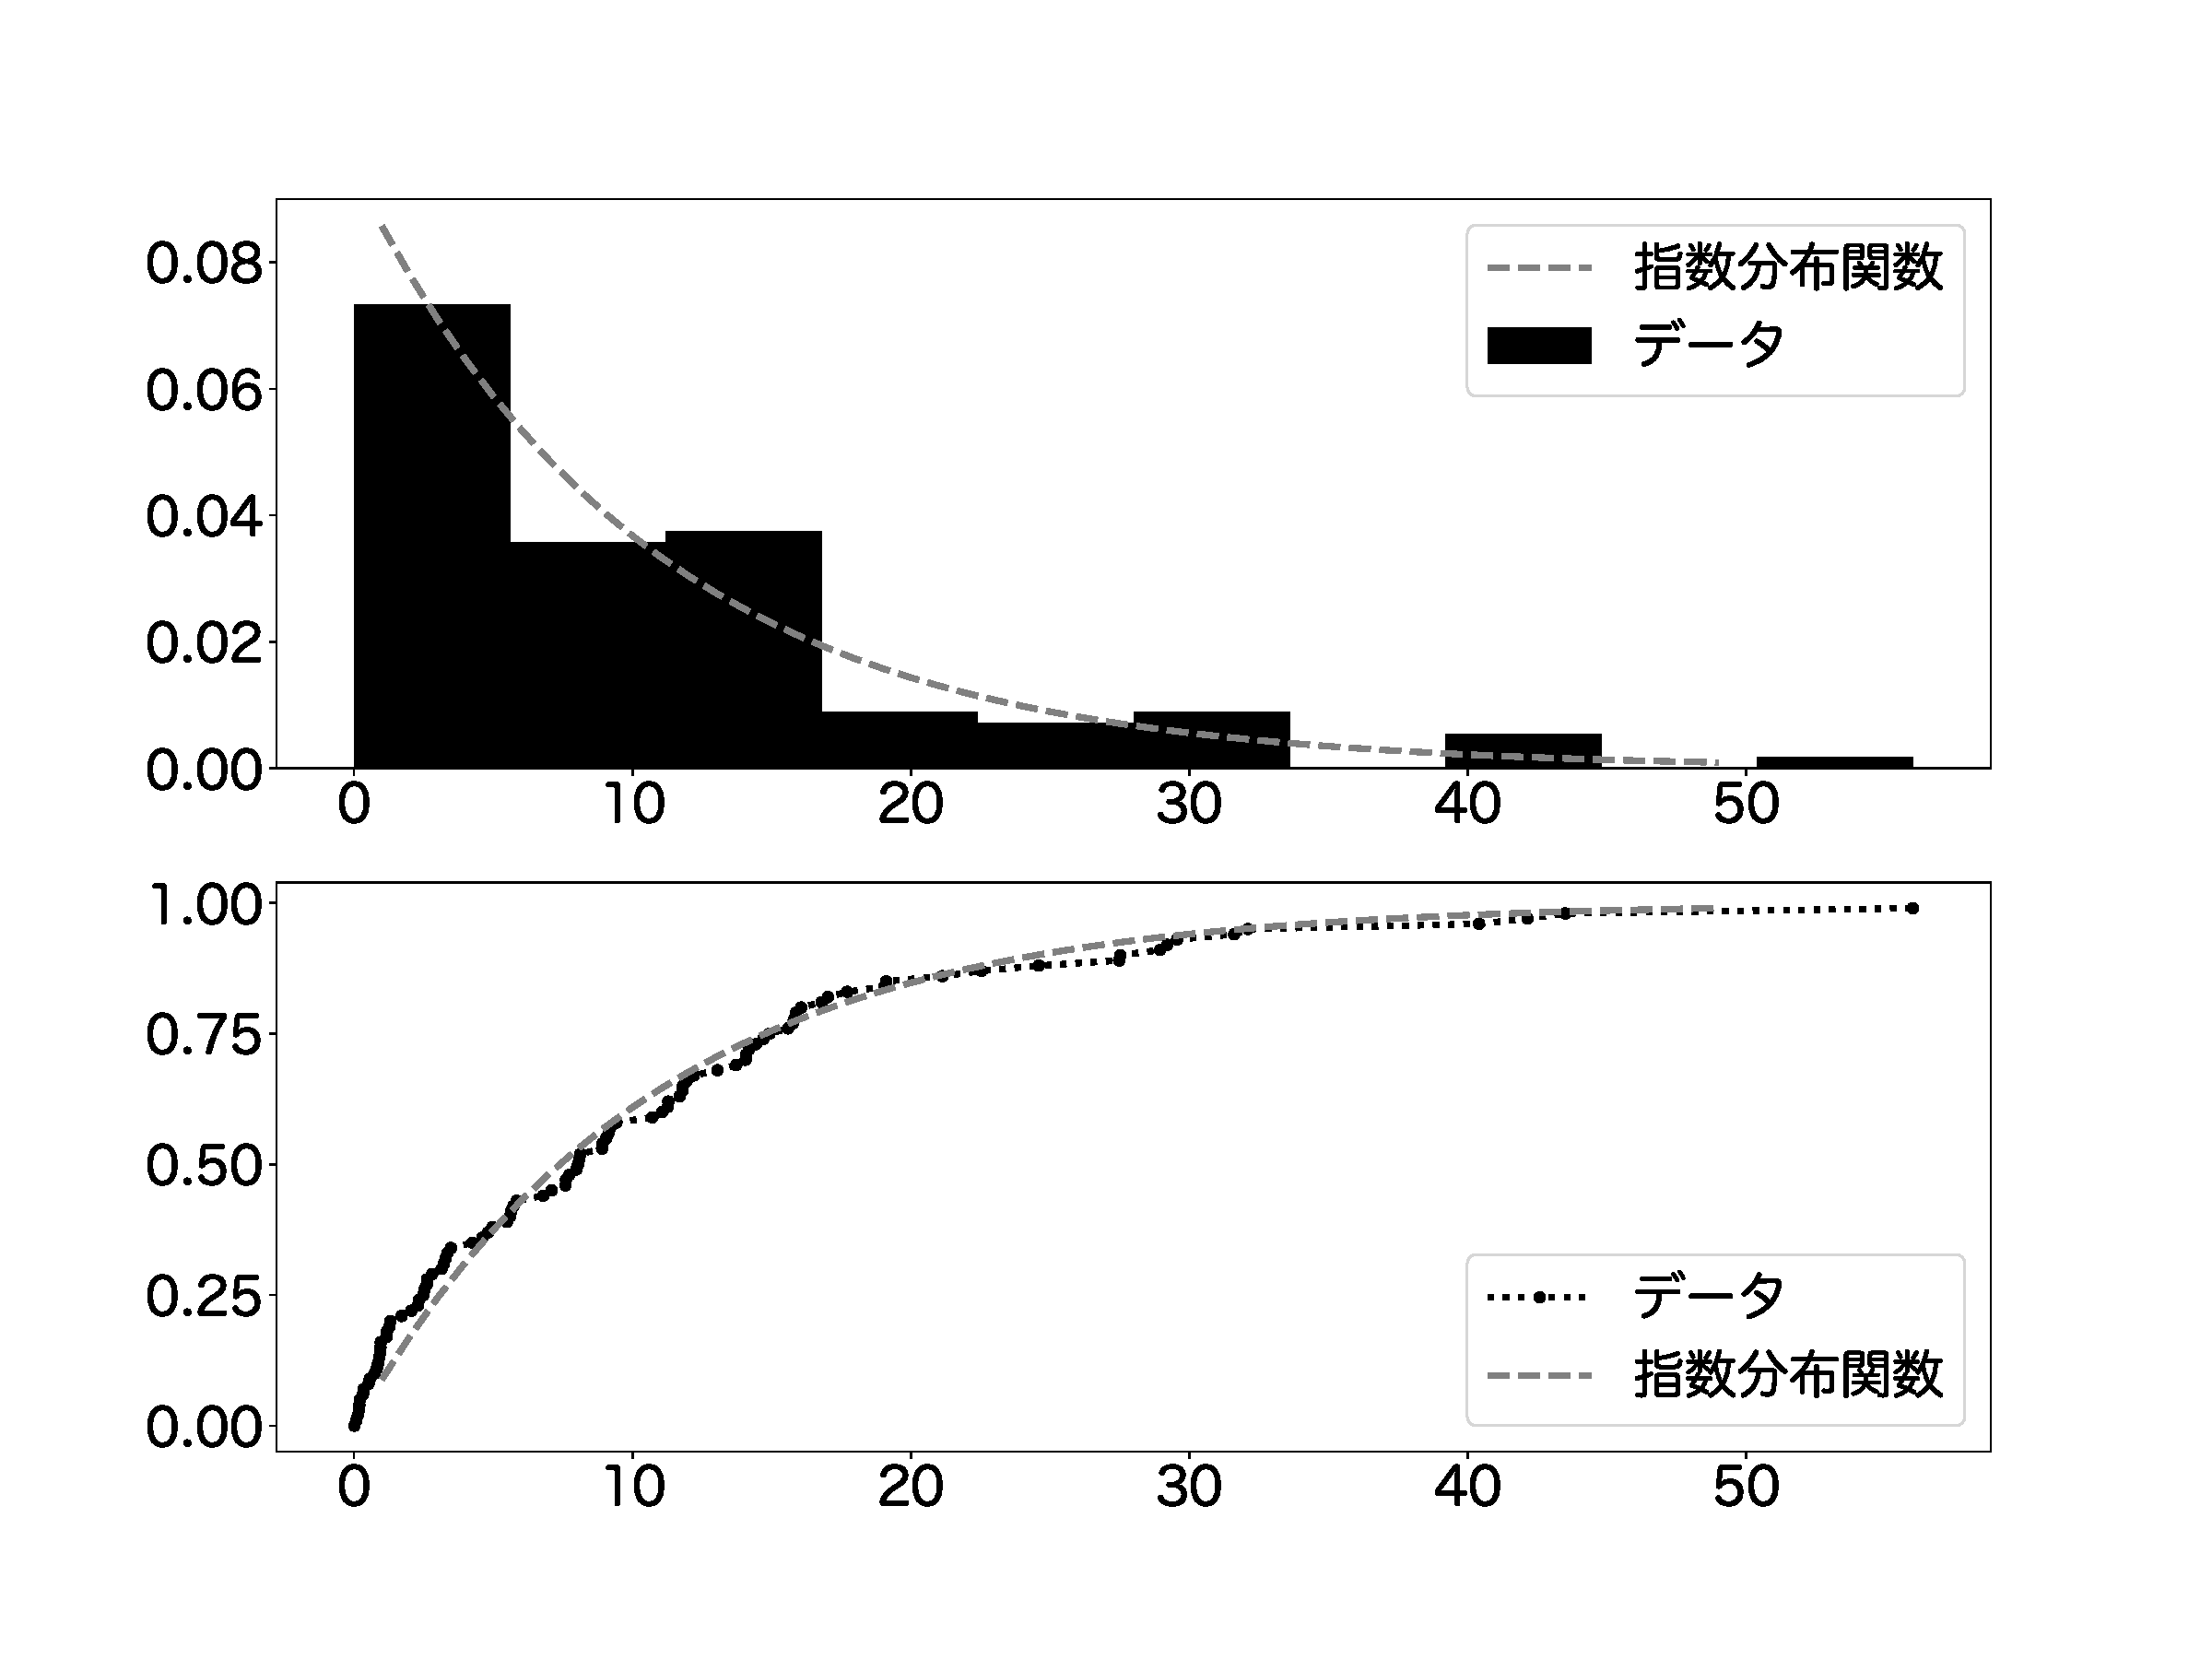
\includegraphics[width=15cm]{../markdown/section1/lambda_0.1.pdf}
    %\caption{しばらくした後の故障頻度の分布図}
\end{center}
\end{figure}





以上を通じて、単純に正規分布を仮定したモデルを導入すれば良し!とは言えないことがわかっただろう。言い換えれば、サンプルサイズが増えたときに見えてくる分布関数から母集団の構造を想定し、統計モデルを構築するべきだという方針が理解できる。
また、データの構造を理解した上で、推測を行うことで、データと推測が程よく一致することがわかった。


% https://biolab.sakura.ne.jp/small-sample-t-test-glm.html
\if 0
AICでモデルを選ぶと、正規分布の仮定がある。指数関数に対しては選択できないのでは? 
\fi
% https://eprints.lib.hokudai.ac.jp/dspace/bitstream/2115/49477/6/kubostat2008e.pdf
% http://www.ieice-hbkb.org/files/01/01gun_12hen_01.pdf




\paragraph{AAA}
あるとき、「改良することで故障日が伸びたみたいなんだ。調査してくれ」と依頼された。サンプルサイズは10程度であり、以下のようになった(今回も指数分布を使ってデータを生成した。もちろん実際の現象は数学の関数で生成されているわけではない)。

\begin{lstlisting}
6.46239039  7.5235678  31.84227772  6.73334029  2.9221049   1.84776618  8.7189158   2.97501827 57.78271493 20.51976339
\end{lstlisting}

統計モデルを構築しよう。
\begin{quote}
    \begin{enumerate}[(1)]
\item i.i.d
\item 正規分布
\item $\mu=10$
\end{enumerate}
\end{quote}

とする。以前のデータ解析では、指数関数を利用し、その平均値は10程度であった。今回の統計モデルでは平均$10$の正規分布を利用することで、この統計モデルが棄却できるかを試してみよう。



\begin{lstlisting}
stats.ttest_1samp(Y, 10)
\end{lstlisting}




その結果、$p=0.421$であることがわかった。このことから、有意水準$p<0.05$を満たしていないので、帰無仮説は棄却で聞いないので、改良できていないという判断を行うべきだろうか?
もちろん良くない。モデルの仮定をみると、統計モデルの仮定(2)が正規分布になっている。これは、我々が扱っている標本にはうまく適応できないことが経験的に理解してきた。
では、次のモデルはどうでしょう。

\begin{quote}
    \begin{enumerate}[(1)]
\item i.i.d
\item 指数分布
\item 指数分布の母数$\lambda=0.1$
\end{enumerate}
\end{quote}
このモデルは、故障日をよく予測してくれることがわかっている。
今回、統計モデルが正規分布ではないので、これまでの仮説検定により、統計モデルとデータの乖離を評価できない。そこで、数理統計学の知識を使う。

\subsection{指数分布関数の統計検定}
確率変数$X_1,X_2,\cdots,X_n \sim i.i.d \ Exp(\lambda)$は、$n\bar{X}\sim Ga(1,\frac{1}{\lambda}) $ただし、$\bar{X}=X_1+X_2 \cdots +X_n$ここで、$Ga(1,\lambda)$は、尺度母数$\lambda$のガンマ分布である。統計量$\bar{X}$を利用した検定ができることが示唆される。
%https://ds.machijun.net/clear-exercise-of-statistics/%E7%AC%AC7%E7%AB%A0-%E6%8C%87%E6%95%B0%E6%AF%8D%E9%9B%86%E5%9B%A3ex%CE%BC%EF%BC%89%E3%81%AE%E6%AF%8D%E5%B9%B3%E5%9D%87%E3%81%AE%E4%BF%A1%E9%A0%BC%E5%8C%BA%E9%96%93%E3%81%A8%E6%A4%9C%E5%AE%9Ap128/



\subsection{尤度比検定}
TODO: 尤度比検定の定義

我々のデータをもとに推論をすると、
$$
\eta= \frac{\lambda_0\exp\left({-\lambda_0\sum x_i}\right)}{\bar{\lambda}^n \exp{(-n)}}
$$
ここで、$\bar{\lambda}$は最尤推定量であり、$\frac{n}{\sum x_i}$、$\lambda_0=0.1$,$n$はサンプルサイズである。
以上を元に、$\eta$を計算する。
$$
-2\log \eta \sim \chi^2_1
$$

より、$p=0.1902$と計算できる。$p$値を計算したら、やることはいつも同じで、統計モデルの仮定をもう一度調べる。統計モデルの仮定(1)はおそらく問題ない。統計モデルの仮定(2)は、少しの改良を加えただけなので、母集団の特性はほとんど変わっていなと前提を置いているので、悪くない近似ができることを期待している。統計モデルの仮定(3)は、$\lambda=0.1$である。$p>0.05$より現状では母数$\lambda$が変化しているとは言い切れない。




\begin{lstlisting}
9.70693386 14.74490149 33.03244855 21.8343649  40.73749837
\end{lstlisting}


さらにサンプルサイズが増えた。この場合、$p=0.01325$となり、$p=0.05$の有意水準を満たす。$N$数をどこまで増やすべきだったのだろうか。

TODO いつかかくけど、どこまで増やすんだろうか。
理想的には構造がわかるまで計測できたら嬉しい



\subsection{分散分析}
Section.2で行った分析では、様々な母平均に対して、統計モデルの推定がデータと一致することを確かめた。今回は、ばらつきを変化させ、統計モデルと推定の一致について考えてみよう。
統計モデルを構築しよう。
\begin{quote}
    \begin{enumerate}[(1)]
\item i.i.d
\item 正規分布$N(170,\sigma^2)$
\item 正規分布の母数$\sigma$
\end{enumerate}
\end{quote}
このモデルを、$M(\sigma)$とする。身長を予測するモデルとして、分散を替えてみよう。
Section.2で利用していた$M(5.7)$に対して、$M(10.0)$が現象を推定可能かを検討してみよう。
分布関数を書いてみると、グラフの裾野が広がったことが見て取れる。その分、ピークである$170$のあたりの頻度が減少している。つまり、$170$が出てくる頻度が下がり、より様々な身長の人がサンプリングできることが期待される。一方で、$M(2.0)$では、$170$の辺りが増え、他の場所では、頻度が現象することがわかる。$M(5.7)$よりも、身長のバラエティが少ないデータにたいし適合できる。


\begin{lstlisting}
163.54258776 179.15834405 172.6934295  166.29185695 177.65182141 165.87491547 172.08610141 158.30711988 163.74574501 176.47887419
\end{lstlisting}




拒否するべき統計モデルはどのような母数をもつだろうか。
10人から無作為抽出したデータに対して、統計モデル$M(3.1),M(12.0)$は十分データを説明できるだろうか?
統計モデルの上で、確率変数$X_1,X_2,\cdots,X_n$から計量される以下の統計量を定義する。
$$
Y_0=(n-1)\left(\frac{S_x}{\sigma}\right)^2
$$
ここで、$S_x^2=\frac{1}{n-1}\sum_{i=0}^{n}(x_i-\bar{x})^2,\bar{x}=\frac{1}{n}\sum_{i=0}^{n}x_i$である。
統計量$Y_0$は、$Y_0\sim\chi^2_{n-1}$であることがわかっている(定理\ref{normal_sigma_chi2})。
このとき、$M(3.1),M(12.0)$については、$p<0.05$となり棄却される。
$p$値を基準にして、絶対にだめな統計モデル$M(3.1)$から、サンプリングを行ってみる。
\begin{lstlisting}

165.02227239, 163.16327065, 170.40109545, 170.81675656, 167.80872784, 166.91030856, 167.24096441, 170.44877048, 165.99400494, 167.59131488
\end{lstlisting}

統計モデル$M(5.7)$よりも値が広がった印象があると直ちにはわからない。
$M(3.1)$を使って、$180cm$を超える人の割合を計算すると、$P(X>180)<10^-5$となり、観測と比較してかなり少ない。
同様に、統計モデル$M(12.0)$を使って計算を行うと、$P(X>180)=0.15$となり、観測と比べて多いこともわかる。
棄却されなかった統計モデル$3.1<\sigma<12.0$の中でも、積極的に予測に利用するには、データの構造をより理解する必要がある。


\begin{figure}
\begin{center}
    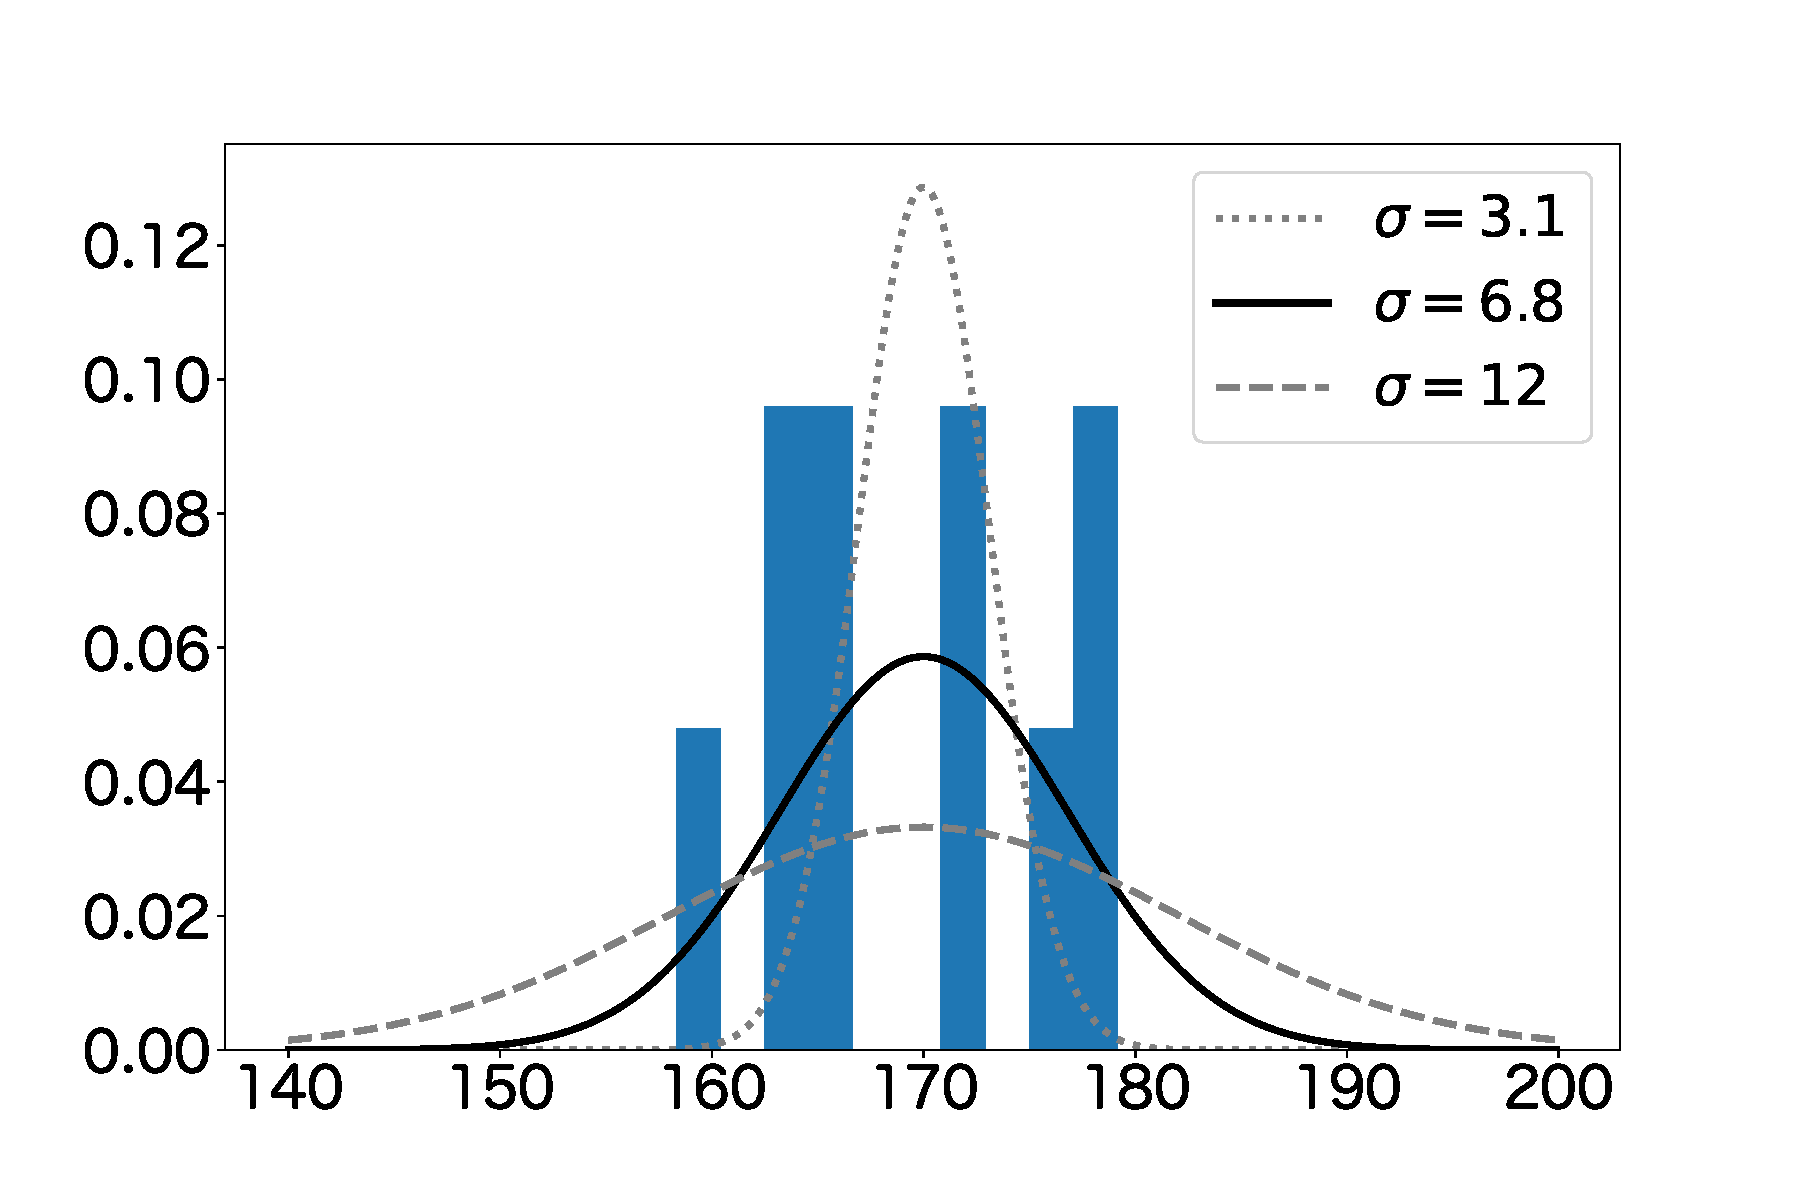
\includegraphics[width=15cm]{../markdown/section1/normal_sigma.pdf}
    %\caption{検出力}
\end{center}
\end{figure}

\if 0
https://biolab.sakura.ne.jp/welch-test.html
https://biolab.sakura.ne.jp/welch-anova-statwing.html
https://biolab.sakura.ne.jp/welch-test.html
\fi

\clearpage
\section{2標本の検定}
\subsection{正規分布を含んだ統計モデル}
我々は普段、男女の身長をみているから男性と女性を同じ統計モデルを用いて推測することは、到底無理だと言える。だが、あえて統計モデルを一つ構築して、男女の身長について推測を試みる。
\begin{quote}
    \begin{enumerate}[(1)]
\item i.i.d
\item 正規分布
\item 正規分布母数$\mu,\sigma=5.7$
\end{enumerate}
\end{quote}
この統計モデルを$M(\mu)$とかく。データを元にして、標準偏差は男女の差がほとんどなく、$5.7$程度であった。男性に対して制度の良い推測を行えていた$M(170)$を使って、女性の身長について推測してみる。女性で、$170cm$以上はどのくらいの頻度で現れるのか、$P(x>170)=0.5$である。一方で、データでは、$0.0179$である。また、平均身長は、データでは$157.8cm$程度である。このことから、統計モデルとデータが乖離していることがわかる。


\if 0
このように、二つの標本が異なることがわかっている、データでは、同じ統計モデルで予測するとデータに一致しないことがわかる。
\fi


以上は、サンプルサイズが十分に大きい場合の平均値と分散を知っているから一つの統計モデルを使って男と女の身長を推測することが難しいことを示唆した。


一方で、サンプルサイズが十分ではない、言い換えれば、分布の特徴が掴みにくい場合、2標本を一つの統計モデルで推測するとまずいことがわかるのだろうか?
男と女、それぞれ5人から計測を行った、上が男、下が女の標本である。
\begin{lstlisting}

[161.92083043 162.3764036  170.60849829 166.64996998 164.83863778]
[159.58195311 152.93245418 159.18632478 145.77567615 152.13809195]
\end{lstlisting}


統計モデルにより、$x_1,x_2,\cdots,x_n$,$y_1,y_2,\cdots,y_n$とサンプリングされたとする。次の統計量を定義する、
$$
Z=(\bar{x}-\bar{y})\frac{\sqrt{mn}}{\sigma\sqrt{m+n}}
$$
ただし、$\bar{x}=\frac{1}{n}\sum_{i=0}^{n} x_i,\bar{y}=\frac{1}{m}\sum_{i=0}^m y_i$である。
$Z$は、$Z\sim N(0,1)$となることがわかっている。

絶対にダメな統計モデルの範囲は、$Z$の大きさ$|Z|$によって決まる。
$p=0.05$とすると、
\begin{eqnarray*}
    &|Z|& < z_{0.025}\\
    &\rightarrow & |\bar{x}-\bar{y}|\frac{\sqrt{mn}}{\sigma\sqrt{m+n}} < z_{0.025}\\
    &\rightarrow& |\bar{x}-\bar{y}| <z_{0.025}\frac{ \sigma\sqrt{m+n} }{ \sqrt{mn }}\\
\end{eqnarray*}


数式を書き換えれば、$|\bar{x}-\bar{y}|$の大きさによって決まることがわかる。
無作為抽出したデータの平均値$\bar{X},\bar{Y}$の差の絶対値がこの範囲に収まらなければ、この統計モデルは、現実を捉えていないと判断され、棄却される。

無作為抽出されたデータを用いて検定にかけてみると、$p=0.004$となり、$p=0.05$よりも小さいことがわかった。
統計モデルの仮説が妥当であることを確認する。仮定(1)は満たされるように無作為抽出を行い計測したので、問題ないと考える。仮定(2)については、サンプルサイズを大きくしたときに、正規分布による予測がよく当たることを知っているので、この仮説も大きく外れているとは言い切れない。最後に、仮説(3)が間違っていることが示唆される。
以上によって、帰無仮説が棄却される。



\begin{lstlisting}
def tTest(X,Y,sigma):
    x_bar,y_bar = np.average(X),np.average(Y)
    M,N = len(X),len(Y)
    Z = (x_bar-y_bar)*np.sqrt(M*N)/(sigma*np.sqrt(M+N))
    p=norm.cdf(Z,0,1)
    return 1-p
tTest(X,Y,5.7)
\end{lstlisting}


\begin{lstlisting}
def rejectRange(X,Y,sigma):
    M,N = len(X),len(Y)
    Z = sigma*(np.sqrt(M+N))/np.sqrt(M*N)
    za,zb= norm.interval(0.95,0,1)
    return Z*za,Z*zb
rejectRange(X,Y,5.7)
\end{lstlisting}
\subsubsection{信頼区間}
平均母数$\mu_1,\mu_2(\mu_1\neq \mu_2)$のときに、式を変形していくと、次がわかる
\begin{equation*}
    (\bar{X}-\bar{Y})-z_{0.025}\sigma\sqrt{\frac{1}{n_1}+\frac{1}{n_2}} \leq \mu_1-\mu_2 \leq (\bar{X}-\bar{Y})+z_{0.025}\sigma\sqrt{\frac{1}{n_1}+\frac{1}{n_2}}.
\end{equation*}
これは、$\bar{X},\bar{Y}$を得たときに、$\mu_1-\mu_2$がこの範囲にあれば、$\mu_1=\mu_2$という統計モデルは棄却できない。

もう一度、式変形をしてみると、次の式を得る。
\begin{equation*}
    (\bar{\mu_1}-\bar{\mu_2})-z_{0.025}\sigma\sqrt{\frac{1}{n_1}+\frac{1}{n_2}} \leq \bar{X}-\bar{Y} \leq (\bar{\mu_1}-\bar{\mu_2})+z_{0.025}\sigma\sqrt{\frac{1}{n_1}+\frac{1}{n_2}}.
\end{equation*}
この式は、標本を繰り返し得ていくと$\bar{X}-\bar{Y}$がこの範囲の中に$95\%$の確率で得られることを示唆している。

\subsubsection{検出力}
二つの統計モデル$M(\mu,\mu),M(\mu_1,\mu_2)$において、$M(\mu,\mu)$を元に、検出力を計算する。
$M(\mu,\mu)$における信頼区間は、統計量を$Z$とすると、
\begin{equation*}
    -z_{\alpha/2}U \leq Z\leq z_{\alpha/2}U
\end{equation*}
ここで、$U=\sqrt{\frac{\sigma^2_1}{n_1}+\frac{\sigma^2_2}{n_2}}$である。
また、$M(\mu_1,\mu_2)$における統計量を$Z$とすると、$Z = \frac{\bar{x}-\bar{y}}{U}\sim N(0,1)$であるので、$a \sim N(\mu_1-\mu_2,U^2)$ならば、
\begin{eqnarray*}
    A &=& \frac{(a-(\mu_1-\mu_2))}{U} \\
      &=& (\mu_1-\mu_2)/U-z_{\alpha/2}
\end{eqnarray*}
同様に、
\begin{eqnarray*}
    B &=& \frac{(b-(\mu_1-\mu_2))}{U} \\
      &=& (\mu_1-\mu_2)/U-z_{\alpha/2}
\end{eqnarray*}
よって、
\begin{equation*}
    \beta = \varPhi(B)-\varPhi(A)
\end{equation*}
である。

\subsection{母分散が未知のときの統計モデル}


\subsubsection{信頼区間}


\subsection{統計的仮説検定の手順}



\subsubsection{分散未知の場合}
%[統計学 講義](http://www3.u-toyama.ac.jp/kkarato/2020/statistics/handout/Statistics[B]-2020-25-0722.pdf)



\section{ノンパラメトリック検定}
\begin{mybox}
    \paragraph{正規分布じゃないからノンパラメトリック!}
    \begin{quote}
        サンプルサイズが大きい場合は、正規性の検定を行い、正規性でないと確認してからノンパラメトリック検定を使うと書いた文献もある\footnote{\url{https://katosei.jsbba.or.jp/view_html.php?aid=1196}.}。
        正規分布に近いとは言えないこともある場合、ノンパラメトリック検定を勧める文献もある \url{ http://j-ca.org/wp/wp-content/uploads/2016/04/5102_51kyo2_so.pdf . 臨床研究における統計学的解析 ─推定と検定の正しい使い方─}
        これらとは反対に、正規性検定をノンパラメトリック検定を利用するときの基準として使うべきでないと主張する論者もいる\footnote{https://biolab.sakura.ne.jp/normality-test-nonparametric.html}。
        ノンパラメトリック検定を勧められたときには、その検定の仮定を調べて、自分のデータと仮定が妥当であることが確認できるならば、ノンパラメトリック検定を使えば良い。
    \end{quote}
\end{mybox}

\subsubsection{Shapiro-Wilk検定}
Shapiro-Wilk検定で使う統計モデルは、次の二つの仮定により構成されている。
\begin{quote}
    \begin{enumerate}[(1)]
\item それぞれが独立に得られる
\item 正規分布
\end{enumerate}
\end{quote}
この検定を使うと、統計モデルの仮定(1)がクリアな場合、(2)が仮定できないと判断されます。つまり、$p$値が小さければ、正規分布ではないことが主張できます。一方で$p$値が大きい場合では、積極的に正規分布であるとは主張できません。

\begin{mybox}
    \begin{quotation}
t検定を使う前提条件としてShapiro-Wilk検定を使うことを推奨している文献があるようです。


統計モデルは真実ではありませんし、各仮定が前提である必要はありません。どのくらい正規分布から離れているかを判定するのは解析者に依存します。

統計モデルには、各変数が独立であることを仮定しますが、この仮定を前提にする統計的な手法の利用は推奨されてません。統計モデルの仮定のうち一つは前提としようと努力をするのですが、独立性については無視する立場があるのも確かです。我々は、統計モデルの仮定は本当に正しいことを要求しません。
\end{quotation}
\end{mybox}

% https://biolab.sakura.ne.jp/welch-anova-statwing.html

% http://ibis.t.u-tokyo.ac.jp/suzuki/lecture/2015/dataanalysis/L8.pdf
% https://biolab.sakura.ne.jp/normality-test-nonparametric.html




\subsubsection{ウィルコクソン(Wilcox)の符号順位検定}
ウィルコクソンの符号順位検定で使う統計モデルを構成する仮定は次の通りです
\begin{quote}
    \begin{enumerate}[(1)]
\item $i=0,\cdots,n$に対して、$Z_i=Y_i-X_i$とする。$Z_i$は互いに独立である。
\item $Z_i$は連続的母集団に従い、共通の中央値$\lambda$に関して対称である。
\end{enumerate}
\end{quote}  

% https://twitter.com/genkuroki/status/1444531128530976770
% https://www.jstage.jst.go.jp/article/psj/30/1/30_30.006/_pdf




\subsubsection{マン・ホイットニーのU検定}
\begin{quote}
    \begin{enumerate}[(1)]
\item 両標本が同じ分布関数から生成された(帰無仮説)
\item 等分散
\end{enumerate}
\end{quote}
ウィルコクソンの順位和検定
% https://ja.wikipedia.org/wiki/マン・ホイットニーのU検定
% https://oku.edu.mie-u.ac.jp/~okumura/stat/brunner-munzel.html



\subsubsection{対応ある t 検定}
1群の(差を作った)検定なので、等分散の仮定は必要ではない。中身が0と比べつ
% https://biolab.sakura.ne.jp/paired-t-test-two-sample-anova.html


\subsubsection{Walchの検定}
% https://biolab.sakura.ne.jp/maxima-welch-test.html
% https://oku.edu.mie-u.ac.jp/~okumura/stat/ttest.html



\section{数理統計の補足}

      

また、母数分散$\sigma$について次が成り立つ。
\begin{theo}\label{normal_sigma_chi2}
    $X_1,X_2,\cdots,X_n \sim N(\mu,\sigma^2)$について、次が成り立つ。
    \begin{equation*}
        Y = (n-1)(\frac{S_x}{\sigma})^2 \sim \chi^2_{n-1}
    \end{equation*}
    ここで、$S^2_x=\frac{1}{n-1}\sum_{i=1}^n(x_i-\bar{x})^2,\bar{x}=\frac{1}{n}\sum_{i=1}^n x_i$である。
\end{theo}


%https://ds.machijun.net/clear-exercise-of-statistics/%E7%AC%AC7%E7%AB%A0-%E6%8C%87%E6%95%B0%E6%AF%8D%E9%9B%86%E5%9B%A3ex%CE%BC%EF%BC%89%E3%81%AE%E6%AF%8D%E5%B9%B3%E5%9D%87%E3%81%AE%E4%BF%A1%E9%A0%BC%E5%8C%BA%E9%96%93%E3%81%A8%E6%A4%9C%E5%AE%9Ap128/


$n$を自然数とし、ガンマ分布$Ga(\frac{n}{2},2)$を特に、カイ2乗分布といい、$\chi ^2_n$で表す。



\begin{theo}
$n$を自然数とする。$G\sim\Gamma(\frac{n}{2},\beta),Y_n\sim \chi^2_n$とすると、$P(G\leq w) = P(Y_n \leq 2\beta w)$
\end{theo}
\begin{proof}
$w >0$に対して、
\begin{eqnarray*}
    P(G \leq w) &=& \int_0^w \frac{\beta^\frac{n}{2}}{\Gamma(n/2)}x^{n/2-1}\exp{(-\beta x)}dx \\
    &=&\int_0^{2\beta w} \frac{\beta^{\frac{n}{2}}}{\Gamma(n/2)}\left( \frac{t}{2\beta} \right)^{n/2-1}\exp{(-\beta t/2\beta)}\frac{dt}{2\beta} (x=t/(2\beta)) \\
    &=& \int_0^{2\beta w} \frac{1}{2^{n/2}\Gamma(n/2)}t^{n/2-1}\exp{(-t/2)}dt\\
    &=&P(Y_n \leq 2\beta w)
\end{eqnarray*}
\end{proof}



$n\bar{x}\sim \Gamma(n,\lambda)$である。このとき、$\lambda$の信頼区間を求める。$\lambda$の下限は、
\begin{equation}
    P(G\leq n\bar{x}) = \frac{\alpha}{2}
\end{equation}
を満たし、$\lambda$の上限は、
\begin{equation}
P(G\leq n\bar{x}) = 1-\frac{\alpha}{2}
\end{equation}
を満たす。
下限の式を変形していく。
\begin{eqnarray*}
    \alpha/2 &=& P(G\leq n\bar{x})  \\
    &=& P(Y_{2n}\leq 2n \lambda_l \bar{x})\\
    &\rightarrow& 2n\lambda \bar{x} = \chi^2_{2n}(1-\alpha/2)\\
    &\rightarrow& \lambda = \frac{\chi^2_{2n}(1-\alpha/2)}{2n\bar{x}}
\end{eqnarray*}
上限についても同様に、
\begin{eqnarray*}
    1-\frac{\alpha}{2} &= & P(G\leq n\bar{x}) \\
    &=& P(Y_{2n}\leq 2n\lambda \bar{x})  \\
    &\rightarrow& 2n\lambda \bar{x} = \chi^2_{2n}(\alpha/2)\\
    &\rightarrow&  \lambda = \frac{\chi^2_{2n}(\alpha/2)}{2n\bar{x}}
\end{eqnarray*}
以上によって、$\frac{1}{\lambda}$の信頼区間は、
\begin{equation}
    \frac{2n\bar{x}}{\chi^2_{2n}(\alpha/2)} \leq \frac{1}{\lambda} \leq \frac{2n\bar{x}}{\chi^2_{2n}(1-\alpha/2)}
\end{equation}



\subsection{2標本・指数分布}
$X_1,X_2,\cdots,X_n \sim i.i.d Exp(\theta_1),Y1,Y_2,\cdots,Y_n \sim i.i.d Exp(\theta_2)$とする。帰無仮説$H_0$を、$H_0:\theta_1=\theta_2$とし、対立仮説$H_1$を、$H_1 : \theta_1 \neq \theta_2$とする。帰無仮説のもとで、尤度関数$L_{H_0}$は、

\begin{equation}
    L_{H_0} = \theta^{-n_1-n_2}\exp\{-\theta^{-1}T\}
\end{equation}
ただし、$T=\sum_{i=0}^n X_i+\sum_{i=0}^n Y_i$である。$\frac{\partial H_0}{\partial\theta}=0$となる$\theta$は、

\begin{equation}
    \frac{\partial H_0}{\partial\theta} = \{ -(n_1+n_2)+\theta^{-1}T \}\theta^{-n_1-n_2-1}\exp(-\theta^{-1}T).
\end{equation}
より、$\theta_0=\frac{T}{n_1+n_2}$である。
$\theta_0$を$L_{H_0}$に代入すると、
\begin{equation}
    L_{H_0} = \theta_0^{-n_1-n_2}\exp(-n_1-n_2).
\end{equation}

同様に、対立仮説のもとで、尤度関数$L_{H_1}$は、
\begin{equation}
    L_{H_1} = \theta_1^{-n_1}\exp(-\frac{n_1}{\theta_1}\bar{x})\theta_2^{-n_2}\exp(-\frac{n_2}{\theta_2}\bar{y})
\end{equation}
$\frac{\partial H_1}{\partial\theta}=0$となる$\theta_1$を計算する。
\begin{equation}
    \frac{\partial H_1}{\partial\theta_1}=\{ -n_1\theta_1^{-n_1-1} \exp(-\frac{n_1}{\theta_1}\bar{x})+n_1\bar{x}\theta_1^{-n_1-2}\exp(-\frac{n_1}{\theta_1}\bar{x})\}\theta_2^{-n_2}\exp(-\frac{n_2}{\theta_2}\bar{y}).
\end{equation}
$ \frac{\partial H_1}{\partial\theta_1}=0$より、$(-n_1+n_1\bar{x}\theta_1^{-1})\theta_1^{-n_1-1}=0$より、$\hat{\theta}_1=\bar{x}$である。同様に、$\hat{\theta}_2=\bar{y}$。
以上によって、$L_{H_1}$は、
\begin{equation}
    L_{H_1}(\hat{\theta}_1,\hat{\theta}_2) = (\hat{\theta}_1)^{-n_1}\exp(-n_1)(\hat{\theta_2})^{-n_2}\exp(-n_2)
\end{equation}
である。

尤度比は、
\begin{eqnarray}
    \varLambda = \frac{L_{H_1}}{L_{H_0}} &=& \frac{ (\hat{\theta}_1)^{-n_1}(\hat{\theta}_2)^{-n_2} \exp(-n_1-n_2)}{ \theta_0^{-n_1-n_2}\exp(-n_2-n_2) }\\
    &=& \left(\frac{\theta_0}{\hat{\theta_0}}\right)^{n_1} \left(\frac{\theta_0}{\hat{\theta_1}} \right)^{n_2}
\end{eqnarray}
尤度比検定より、$-2\log \varLambda \sim\chi^2_1$である。

$Ga(\alpha,\beta)$について、以下が成り立つ
\begin{eqnarray}
    k X &\sim& Ga(\alpha,\beta/k) \\
    \frac{1}{k} X &\sim& Ga(\alpha,k\beta)\\
    \chi^2_{2n}&=&Ga(n,2) 
\end{eqnarray}
以上を使うと、
\begin{eqnarray*}
    n\bar{X} &\sim& Ga(n,\frac{1}{\lambda}) \\
    \frac{n}{2}\bar{X} &\sim&(\frac{n}{2},\frac{1}{\lambda}) \\
    \frac{n}{2\lambda}\bar{X} &\sim& Ga(\frac{n}{2},2)=\chi^2_{n}
\end{eqnarray*}
また、ガンマ分布とベータ分布の関係より、$X_1 \sim Ga(\alpha_1,\beta),X_2\sim Ga(\alpha_2,\beta)$ならば、$\frac{X_1}{X_1+X_2}\sim Beta(\alpha_1,\alpha_2)$である。以上より、
$Z=\frac{n\bar{X}}{n\bar{X}+m\bar{Y}}\sim Beta(n,m)$である。このことから、棄却域($z_1 \leq Z \leq z_2$)を求めることができる。具体的には、
\begin{equation}
    \int_0^{z_1}\frac{1}{B{n,m}}z^{n-1}(1-z)^{m-1}dz = \alpha/2,      \int_{z_2}^{\infty}\frac{1}{B{n,m}}z^{n-1}(1-z)^{m-1}dz = \alpha/2.
\end{equation}
この解$z_1,z_2$を計算すれば良い。






%https://stats.stackexchange.com/questions/81151/likelihood-ratio-for-two-sample-exponential-distribution
%https://stats.stackexchange.com/questions/81151/likelihood-ratio-for-two-sample-exponential-distribution


\subsection{中心極限定理}
中心極限定理は本書の内容を超えるので、あえて紹介を避けてきた。一般的な統計学の本には詳細が書かれているので、そちらを読んだ方が良い。
\begin{theo}[中心極限定理]
    期待値$\mu$と分散$\sigma^2$を持つ独立分布に従う確率変数列$X_1,X_2,\cdots$に対し、$S_n=\sum_{k=1}^nX_k$とおくと、
    $S_n$は、期待値$0$、分散$1$の正規分布に分布収束する。
\end{theo}

統計学のユーザーの中には、次のことが成立すると考えている\footnote{
    中心極限仮説が成り立つと考えている人は多い。
    \url{http://www.ner.takushoku-u.ac.jp/masano/class_material/waseda/keiryo/R10_inference.html#3_%E4%B8%AD%E5%BF%83%E6%A5%B5%E9%99%90%E5%AE%9A%E7%90%86} .
    \url{https://yukiyanai.github.io/stat2/clt.html}.
    }。
\begin{hypoth}[中心極限仮説]
    一般のデータについて、データのサンプルサイズを大きくすると、その平均$\bar{x}$は、$\bar{x}\sim N(\mu,\sigma^2/n)$。
\end{hypoth}
反例がすぐに出てくるので、このような仮説は一般には成り立たない。例えば、データがコーシー分布から生成されている場合、成り立たない。

少なくとも一人は、次のように考えていた。
\begin{hypoth}[中心極限仮説2]
    サンプルサイズを大きくすると、正規分布に近づく。
\end{hypoth}
これも間違いである。中心極限定理の前提のもと、標本平均を集めると正規分布に近づくことはありえる。



\subsubsection{ サンプルサイズが大きくなるとデータの構造がわかる}
サンプルサイズが増えると、正規分布を仮定できると書いてある文献もあるが、これは大数極限定理が成立する状況に限られるので、一般の母集団の特徴は正規分布を仮定した統計モデルで捉えるられるとは言い切れない。

\if 0
信頼区間が狭くなるというふうに書いてあることもあるが、これも正しくないはず。
Cauchy分布を使って確かめてみる。
\fi 

サンプルサイズが増えることの利点として、おおよその分布の形がわかるということが挙げられる。
分布の形がわかれば、尤度ひを使った検定が可能になり、棄却すべき統計モデルがわかるようになる。
このことは、研究をさらに進めるさいに、どのような統計モデルを構築すれば良いのかの指針となりうる。
もう一つ利点をあげるなら、比較したい分布との違いを表示することで明らかにできるという点である。
言い換えると、少数のサンプルサイズのときに検定を使うことで、統計モデルの母数を検定することに意味があったのだが、
サンプルサイズが大きくなることで、プロットすれば分布の形の違いが現れるので、検定する意味がなくなる。




\if 0
一方で、データの分布形を判断しようという意見も当然出ている。
\url{https://www.shindanyaku.net/statistics/vol_05/index.php}
\fi 

\if 0
統計学では、あえてデータが正規分布しているという統計モデルを設定し、その統計モデルを使って推測を行います。

https://www.ncchd.go.jp/press/2017/adultheight.html
https://jech.bmj.com/content/71/10/1014.long

\fi 


\bibliography{ref} %hoge.bibから拡張子を外した名前
\bibliographystyle{junsrt}

\end{document}